\documentclass[english]{atlasnote}
\usepackage{atlasphysics} % Contains useful shortcuts. Uncomment to use
\RequirePackage{lineno} \setlength{\linenumbersep}{4pt}
\usepackage{graphicx}
\usepackage{float}
\usepackage{amssymb}
\usepackage{url}
\usepackage{cancel}
\usepackage{morefloats}
\usepackage{harpoon}
\usepackage{caption}
\usepackage{subcaption}
\usepackage{amsmath}
\usepackage{MnSymbol}
\usepackage{multirow}
\usepackage{enumitem}
\usepackage[colorlinks,breaklinks]{hyperref}
\hypersetup{linkcolor=blue,citecolor=blue,filecolor=black,urlcolor=blue}
\usepackage{babel}
\skipbeforetitle{50pt}
\newcommand{\dd}[2]{\frac{\partial{#1}}{\partial{#2}}}

\title{ Measurement of multi-particle azimuthal correlation in proton-lead and proton-proton collisions with the ATLAS detector }

\usepackage{authblk}\renewcommand{\Authands}{, } % avoid ``. and'' for last author
\renewcommand{\Affilfont}{\itshape\small} % affiliation formatting
\author[a]{Mingliang Zhou}
\author[a,b]{Jiangyong Jia}
\author[c]{Adam Trzupek}
\author[a]{Peng Huo}
\affil[a]{Department of Chemistry,Stony Brook University, Stony Brook, NY 11794, USA}
\affil[b]{Brookhaven National Laboratory, Physics Department, Bldg. 510A, Upton, NY 11973, United States of America}
\affil[c]{Institute of Nuclear Physics Polish Academy of Sciences, Krakow}

\newcommand{\lr}[1]{\left\langle #1\right\rangle}

\draftversion{2}

\abstracttext{This note presents details of the analysis of the multi-particle azimuthal anisotropy of charged particles produced in $pp$ and $p$+Pb collisions with the new sub-event multi-particle cumulant method. Cumulant has previously been measured in $p$+Pb and Pb+Pb collision systems, and recently was first measured in $pp$ collision by CMS collaboration. In this note we will show that the traditional cumulant measurement is very sensitive to the multiplicity fluctuation, and existed results might not indicate collectivity even with presence of negative $C_{2}\{4\}$. For this reason, we proposed a new sub-event method within the cumulant framework to further suppress the non-flow in small systems. This new method has been validated in PYTHIA sample, where $C_{2}\{4\}$ calculated from the new method is much closer to 0 than the traditional method. The 4-particle cumulant are calculated for high multiplicity $pp$ data at $\sqrt{s}=13$ TeV as well as 5.02 TeV. Results from the new method give negative $C_{2}\{4\}$ down to 40 tracks, and the values of $C_{2}\{4\}$ are independent of multiplicity fluctuation. The new results indicate potential collective behavior in small collision system.}




\begin{document}
\tableofcontents
\clearpage

List of contributions
\begin{itemize}
\item \verb|Mingliang Zhou|
\begin{itemize}
\item Submit production jobs for 13 TeV $pp$, 5.02 TeV $pp$ and 5.02 TeV $p$+Pb;
\item Development and optimization of the method for sub-event cumulant method;
\item Evaluation of the systematic uncertainties in all systems;
\item Writing the internal note;
\end{itemize}
\item \verb|Jiangyong Jia|
\begin{itemize}
\item Development and optimization of the method for sub-event cumulant method;
\item Evaluation of the systematic uncertainties in all systems;
\item Producing the final physics plots;
\item Writing the paper draft;
\end{itemize}
\item \verb|Adam Trzupek|
\begin{itemize}
\item Analyzer for the results and systematics from traditional cumulant method;
\end{itemize}
\item \verb|Peng Huo|
\begin{itemize}
\item Submit production jobs for 13 TeV $pp$, 5.02 TeV $pp$ and 5.02 TeV $p$+Pb;
\item Cross-check of the subevent analysis code;
\end{itemize}
\end{itemize}
\clearpage

\section{Introduction}
\label{sec:intro}
High energy heavy-ion collisions at RHIC and LHC create a strongly-interacting nuclear matter that exhibit many interesting characteristics. One of which is the collimated emission of particle pairs with small azimuthal-angle separation, $\Delta\phi$, that extends over large range of pseudorapidity differences, $\Delta\eta$. This so called "ridge" correlation was first observed in A+A collisions~\cite{Adare:2008ae, Abelev:2009af, Alver:2009id, ALICE:2011ab, Aad:2012bu, Chatrchyan:2013kba}, but later was also observed in proton-nucleus and light-ion-nucleus collisions~\cite{CMS:2012qk, Abelev:2012ola, Aad:2012gla, Adare:2013piz, Aad:2014lta, Khachatryan:2015waa}, and more recently also observed in high multiplicity proton-proton collisions~\cite{Khachatryan:2010gv, Aad:2015gqa, Aaboud:2016yar, atlas:4}. In A+A collisions, the ridge is believed to be the consequence of collective emission of particles in the azimuthal direction, and the collectivity is generated in the final state after local thermalization, described by relativistic viscous hydrodynamic models. For small system such as $pp$ and $p$+A collisions, the origin of the ridge is less clear. There are considerable debates in the theoretical community on whether the ridge in small systems is of hydrodynamic origin similar to A+A collisions~\cite{Bozek:2013uha} or it is created in the initial state due to gluon saturation effects~\cite{Dusling:2013qoz}.

The ridge signal from two-particle correlation (2PC) is characterized by a Fourier decomposition $\sim 1+2 v_{n}^{2}\text{cos}(n\Delta\phi)$, where the $v_{n}$ denotes the single-particle anisotropy harmonics. The second-order coefficient $v_{2}$ is by far the largest, followed by $v_{3}$. In small collision systems, the extraction of ridge signal requires a careful removal of a large contribution from dijets, which is estimated from 2PC in very low multiplicity events and then subtracted from higher multiplicity events~\cite{Abelev:2012ola, Aad:2012gla, Aad:2014lta, Aad:2015gqa, Aaboud:2016yar, Khachatryan:2016txc}. On the other hand, since collectivity is intrinsically a multi-particle phenomenon, it can be probed more directly using multi-particle correlation (or cumulant) technique~\cite{Borghini:2000sa}. One of the perceived hallmark feature of collectivity is the observation of positively defined signal from $2k$-particle correlation $v_{2}\{2k\},k\ge 2$. The $v_{2}\{4\}$ and $v_{2}\{6\}$ have been measured in high-multiplicity $pp$ and $p$+Pb collisions~\cite{Khachatryan:2015waa, atlas:4, Khachatryan:2016txc, Aad:2013fja}. However, this perception is quite misleading in small collision systems, where the non-flow correlation can be as large or bigger than genuine long-range ridge correlation. Recently, an improved cumulant method based on $\eta$-separated sub-events has been proposed to further reduce the non-flow correlations, in particular from jets  and dijets~\cite{jjia}. The performance of the method in suppressing non-flow correlations has been validated using PYTHIA 8 model, which contains no long-range collective effects.

Multi-particle cumulants suppress jet and short-range correlations, but not completely removing it. In fact $v_{2}\{4\}$ is observed to flip sign at smaller $N_{ch}$, number of charged particle, in $pp$ and $p$+Pb collisions. Recently ATLAS observed that the $N_{ch}$ value where sign-flip happens and the magnitude of $v_{2}\{4\}$ depend also on how the event class are chosen for the calculation of cumulants. In this paper, we show that the choice of event class influences the probability of non-flow, and consequently the non-flow distribution to the $v_{2}\{4\}$. An improved cumulant method is proposed to further suppress non-flow, and therefore reduce the sensitivity to non-flow fluctuations. In this method, cumulants are constructed from particles in several subevents separated in $\eta$, which allows measurement of multi-particle correlations to much lower $N_{ch}$.

The structure of the internal note is as follows. In section~\ref{sec:mtd} subevent cumulant will be briefly introduced, with all the formulas listed. In section~\ref{sec:evtSlc}, data sets together with event and track selections will be described. Detailed procedures of the analysis will be presented in section~\ref{sec:ana}. In section~\ref{sec:sys}, we will discuss all the primary systematics and cross-checks. In section~\ref{sec:result}, all the physics plots in different collision systems will be shown. Section~\ref{sec:summary} summarizes the whole analysis.







\clearpage

\section{Sub-event multi-particle cumulants}
\label{sec:mtd}
\subsection{Basic idea of subevent cumulant}
In this analysis we focus mainly on four-particle subevent cumulant, but the generalization to higher-order is straightforward. The basic idea for subevent cumulants is shown in Fig.~\ref{fig:subevt_demo}. The event is equally divided into three non-overlapping rapidity ranges, labelled as $A$, $B$ and $C$. In this analysis, $A$ is defined with $-2.5/3<\eta<2.5/3$, $B$ is defined with $-2.5<\eta<-2.5/3$ and $C$ is defined with $2.5/3<\eta<2.5$. Four-particle correlators are then constructed by choosing two particles from subevent $A$ and one particle each from subevents $B$ and $C$. All other permutations are also considered to increase the number of pairs (e.g. two particles from subevent $B$ and one particle each from subevent $A$ and $C$). Dijets contributions, the main source for non-flow, are suppressed, since they can only produce particles in each subevent. For comparison, we also consider cumulants based on two subevents as shown in Fig.~\ref{fig:subevt_demo}. In this case, two particles each are chosen from $A$ and $B$, which effectively suppress contribution from single jet, but not away-side jets when it lands in different subevents. For the 2 subevent, in this analysis, $A$ is defined with $\eta<0$ and $B$ is defined with $\eta>0$.

\begin{figure}[H]
\centering
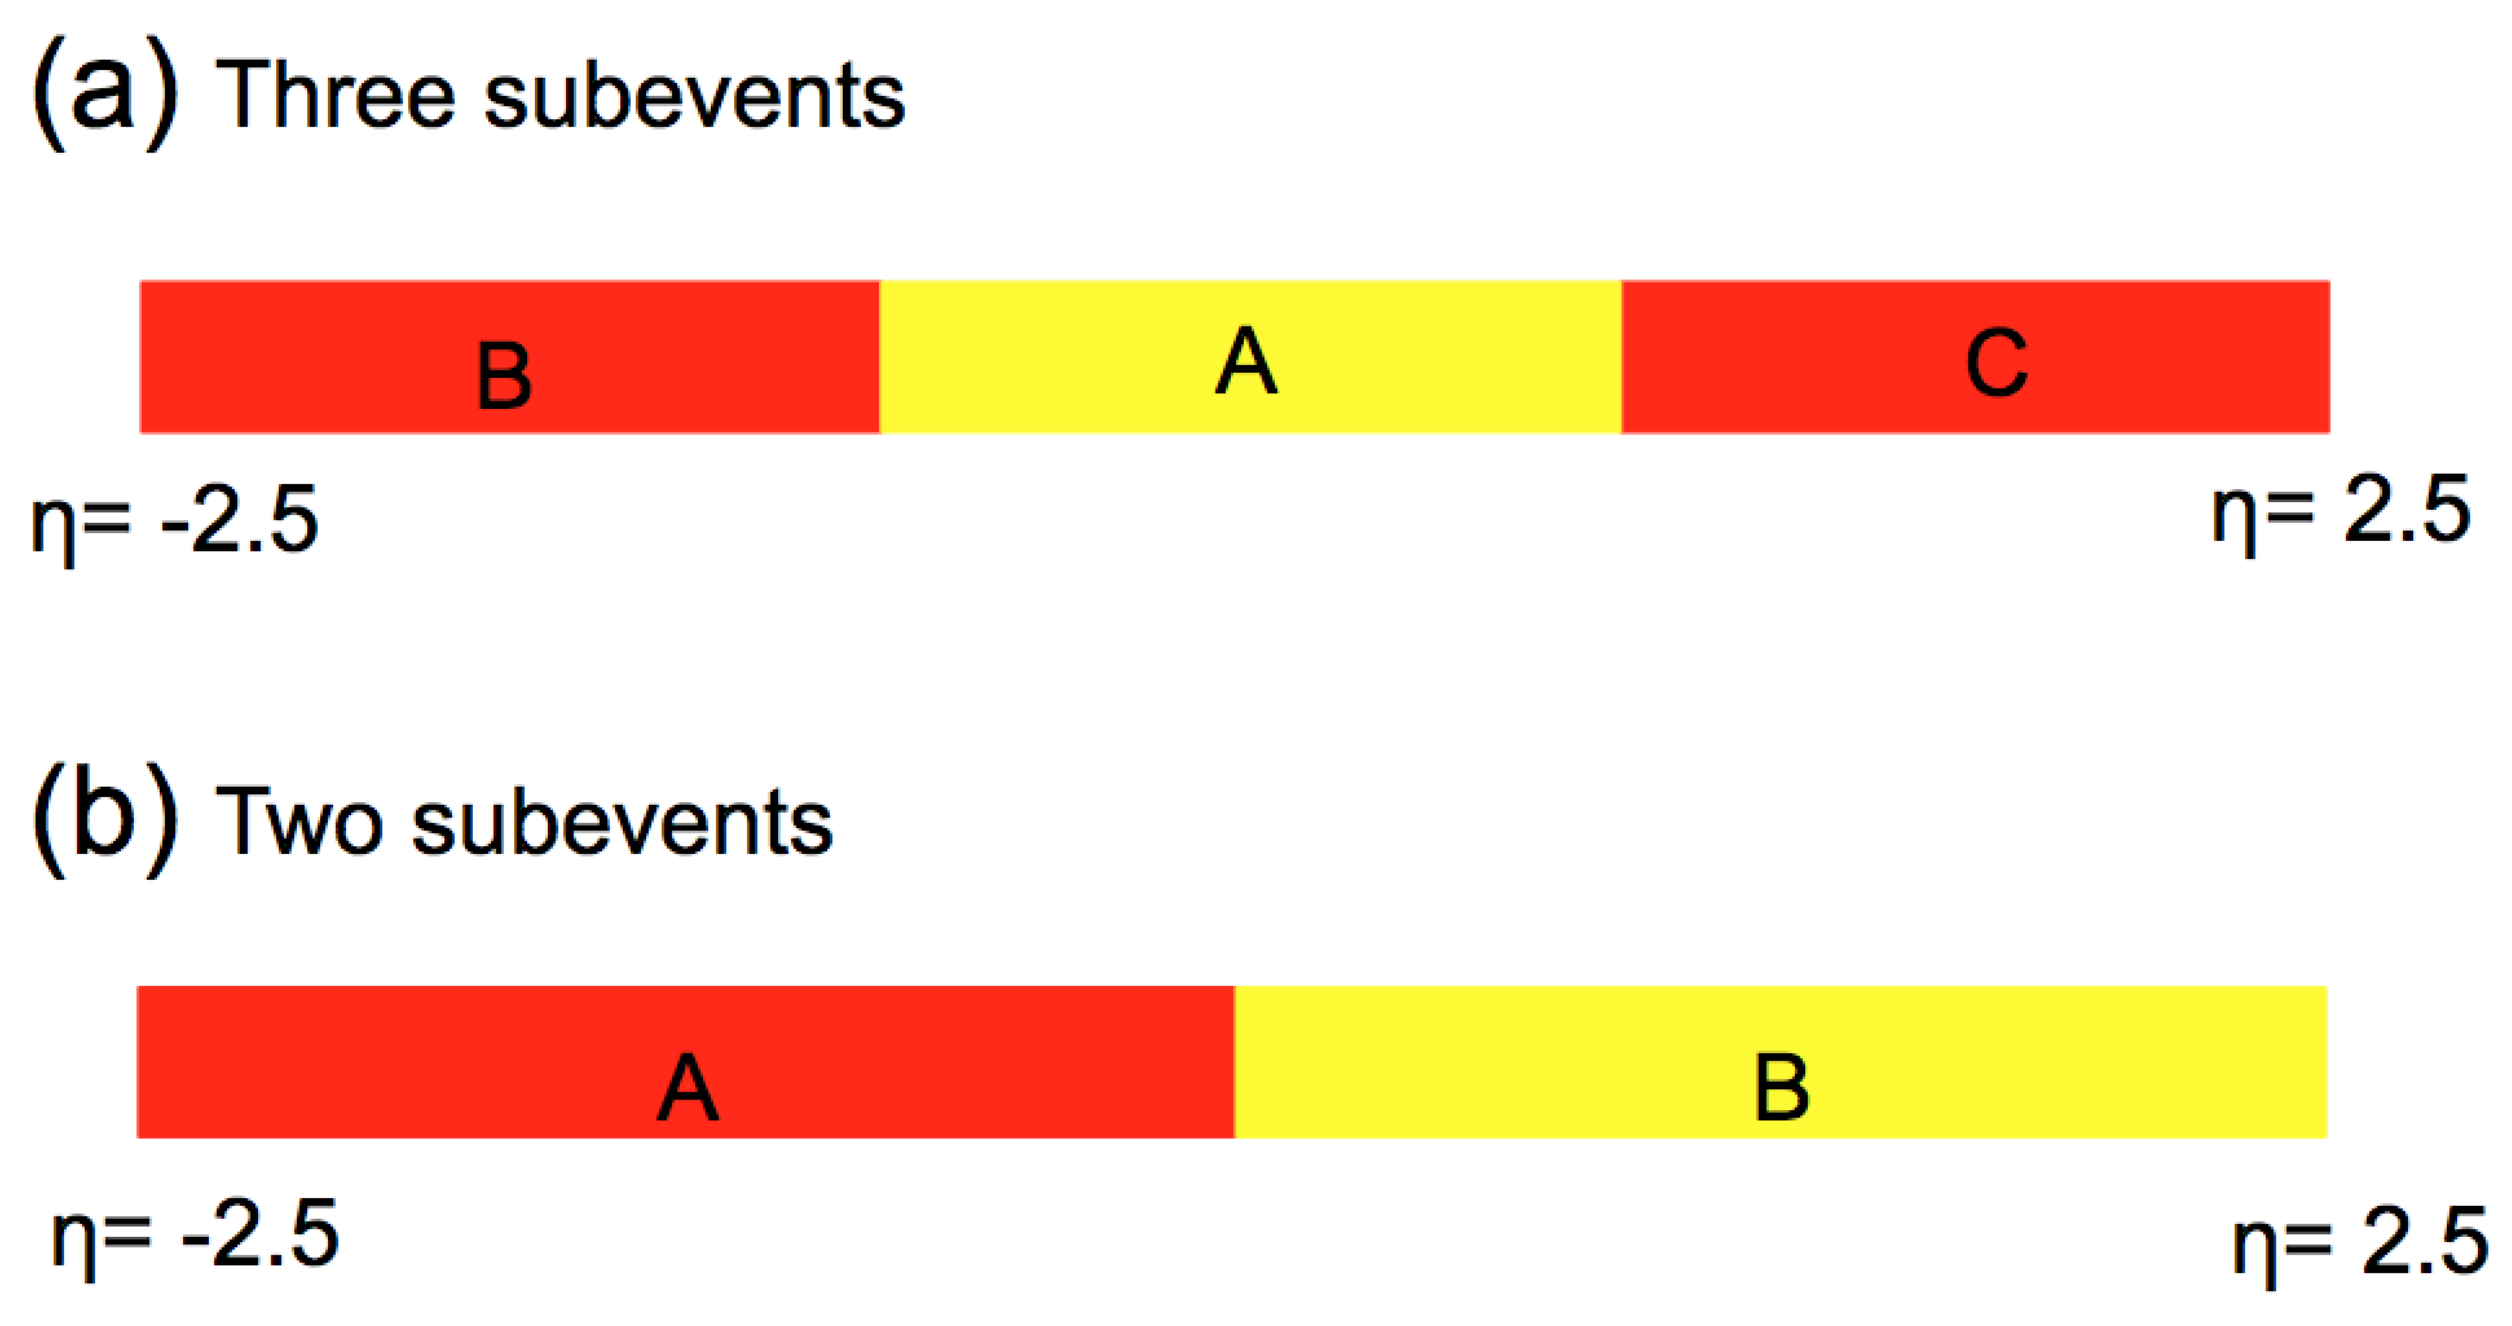
\includegraphics[width=0.7\columnwidth]{figs/sec_mtd/subevt_demo.png}
\caption{The $\eta$ ranges for the subevents in three-subevent method (a) and two-subevent method (b).}
\label{fig:subevt_demo}
\end{figure}

In this section, we will quickly go over all the formulas used for the analysis. Detailed descriptions will be discussed in the reference method paper~\cite{jjia}.

\subsection{Traditional cumulant}
Compared with newly developed subevent cumulant, the existing cumulant method is referred as traditional cumulant, where the 4-particle cumulant is defined as:
\begin{equation}
C_{n}\{4\}\equiv \lr{4}-2\lr{2}^{2}
\end{equation}
Using the direct or Q-cumulant technique, 4-particle correlation $\lr{4}$ and 2-particle correlation $\lr{2}$ are defined as~\cite{Bilandzic:2010jr, Bilandzic:2013kga}:
\begin{equation}
\begin{split}
\lr{2}&\equiv \frac{|Q_{n}|^{2}-M}{M(M-1)} \\
\lr{4}&\equiv \frac{|Q_{n}|^{4}+|Q_{2n}|^{2}-2\text{Re}(Q_{2n}Q_{n}^{*}Q_{n}^{*})-4(M-2)|Q_{n}|^{2}+2M(M-3)}{M(M-1)(M-2)(M-3)}
\end{split}
\end{equation}
where $M$ is the multiplicity in each event and $Q_{n}$ is calculated event-by-event:
\begin{equation}
Q_{n}\equiv\sum_{i}e^{in\phi_{i}}
\end{equation}
and without special mention, in this analysis, only the real part of the inner products (e.g. $Q_{2n}^{2}-2Q_{2n}Q_{n}^{*}Q_{n}^{*}$) is taken.



\subsection{2 sub-event method}
The cumulant is defined in a way that the non-flow sources associated with lower number of particles will be subtracted. Since in the framework of sub-event cumulant, the way non-flow sources are correlated is changed, the corresponding cumulant definition also needs to be changed:
\begin{equation}
C_{n}^{a,a|b,b}\{4\}\equiv \lr{4}_{a.a|b,b}-2\lr{2}_{a|b}^{2}
\end{equation}
where subscript $a,a|b,b$ defines how the four particles are arranged in the two sub-events. In this type, particles in the same sub-events are always correlated with particles in the other sub-events. In other words, particles in the same sub-events will not be correlated with each other, so that the short-range non-flow sources are suppressed. There will be an alternative arrangement for 2 sub-event cumulant: $a,b|a,b$. In this analysis, we will only discuss the first type $a,a|b,b$ since there are less residual non-flow contribution compared with the other type.

Following similar direct cumulant technique, 4-particle correlation $\lr{4}_{a,a|b,b}$ and 2-particle correlation $\lr{2}_{a|b}$ can be calculated in a single event loop:
\begin{equation}
\begin{split}
\lr{2}_{a|b}&\equiv \frac{Q_{n,a}Q_{n,b}}{M_{a}M_{b}} \\
\lr{4}_{a,a|b,b}&\equiv \frac{(Q_{n,a}^{2}-Q_{2n,a})(Q_{n,b}^{2}-Q_{2n,b})^{*}}{M_{a}(M_{a}-1)M_{b}(M_{b}-1)}
\end{split}
\end{equation}
where $M_{a}$ and $M_{b}$ are number of particles in each sub-event. $Q_{n,a}$ and $Q_{n,b}$ are the Q-vector in each sub-event, where the definition is same as the traditional cumulant.



\subsection{3 sub-event method}
Similar as the 2 sub-event method, depending on how the particles are correlated between sub-events, there are two types for the cumulant definition: $C_{n}^{a,a|b,c}\{4\}$ and $C_{n}^{a,b|a,c}\{4\}$. For the same reason as 2 sub-event method, we only consider the first type, where there is no correlation within the sub-event. The definition of the 4-particle 3 sub-event cumulant $C_{n}^{a,b|a,c}$ is:
\begin{equation}
C_{n}^{a,a|b,c}\{4\} \equiv \lr{4}_{a,a|b,c}-2\lr{2}_{a|b}\lr{2}_{a|c}
\end{equation}
where subscript $a,b|a,c$ defines how the four particles are arranged in the two sub-events: 2 particles from sub-event A and the other two from B and C separately. It is worth mentioning that there are two unique combinations by rotating the sub-event A, B and C, which will contribute to the total number of pairs.

Similarly, 4-particle correlation $\lr{4}_{a,a|b,c}$ and 2-particle correlation $\lr{2}_{a|b}$ and $\lr{2}_{a|c}$ can be calculated using the direct cumulant technique:
\begin{equation}
\begin{split}
\lr{2}_{a|b}&\equiv \frac{Q_{n,a}Q_{n,b}}{M_{a}M_{b}} \\
\lr{2}_{a|c}&\equiv \frac{Q_{n,a}Q_{n,c}}{M_{a}M_{c}} \\
\lr{4}_{a,a|b,c}&\equiv \frac{(Q_{n,a}^{2}-Q_{2n,a})Q_{n,b}^{*}Q_{n,c}^{*}}{M_{a}(M_{a}-1)M_{b}M_{c}}
\end{split}
\end{equation}
where the definitions are the same as 2 sub-event method.

All the formulas in this section are without particles weights. The formulas with particle weights (tracking efficiency and detector effects) will be introduced in the following section~\cite{Abelev:2014mda}. In this analysis, we will only focus on the 4-particle cumulant. One reason is that due to the large statistical errors, it is not practical to measure 6-particle cumulant in small systems like $pp$. But the main reason is that traditional cumulant relies on correlation of more particles to suppress the non-flow sources, since non-flow source is usually associated with few particles. However, this is not true for sub-event method. By purposely put the particles into sub-events extended in a wide $\eta$ range, the non-flow correlation is already suppressed. In other word, the advantage of sub-event method is to suppress the non-flow without involving more particles. For these reasons, we will only discuss the results of 4-particle cumulants in this note. 




\clearpage

\section{Data samples, event and tracking selections}
\label{sec:evtSlc}
\subsection{$pp$ 13 TeV}
In 2015 and 2016, low-$\mu$ and intermediate-$\mu$ $pp$ data was collected with ATLAS detectors~\cite{Aad:2008zzm}. An additional pixel layer, the "Insertable B Layer" (IBL)~\cite{atlas:1, atlas:2} installed between Run 1 and Run 2, is used in the $pp$ measurement. There are four run periods depending on the triggers used and they will be discussed in the following sections.

The good events are selected by Good-Run-List and with $|z_{vtx}|<150 $mm.

To reduce the fraction of fake tracks, standard track selection has been applied:
\begin{itemize}
\item Tracks are from primary vertex
\item If IBL hit is expected: at least 1 IBL hit
\item If on IBL hit is expected: a Layer-0 hit if expected
\item At least 1 pixel hit + dead sensors
\item $p_{T}<300$ MeV: at least 2 SCT hits + dead sensors
\item $p_{T}<400$ MeV: at least 4 SCT hits + dead sensors
\item $p_{T}>400$ MeV: at least 6 SCT hits + dead sensors
\item If $p_{T}>10$ GeV: $\chi^{2}$ probability $<0.01$
\item $|d_{0}|<1.5$
\item $|z_{0}-v_{z}|\text{sin}\theta<1.5$
\item $|\eta|\le 2.5$
\item $p_{T}\ge 200$ MeV
\end{itemize}
In the section of systematics, the selection will be tightened to check the stability of the results.



\subsubsection{Run period 1}
Low-$\mu$ data was collected in June and intermediate-$\mu$ data was collected in October. All the runs, with Good Run List (GRL) selections, are included in this analysis and they are listed as below:

\begin{itemize}

\item Run 267358, peak $\mu=0.00255$, 8.6 million events
\begin{itemize}[leftmargin=*]
\item[] \verb|data15_13TeV.00267358.physics_MinBias.merge.AOD.f597_m1441|
\end{itemize}

\item Run 267359, peak $\mu=0.00612$, 12.3 million events
\begin{itemize}[leftmargin=*]
\item[] \verb|data15_13TeV.00267359.physics_MinBias.merge.AOD.f597_m1441|
\end{itemize}

\item Run 267360, peak $\mu=0.374$, 12.6 million events
\begin{itemize}[leftmargin=*]
\item[] \verb|data15_13TeV.00267360.physics_MinBias.merge.AOD.f597_m1441|
\end{itemize}

\item Run 267367, peak $\mu=0.46$, 17.1 million events
\begin{itemize}[leftmargin=*]
\item[] \verb|data15_13TeV.00267367.physics_MinBias.merge.AOD.f597_m1441|
\end{itemize}

\item Run 267385, peak $\mu=0.466$, 71.2 million events
\begin{itemize}[leftmargin=*]
\item[] \verb|data15_13TeV.00267385.physics_MinBias.merge.AOD.f597_m1441|
\end{itemize}

\item Run 267599, peak $\mu=0.488$, 105.6 million events
\begin{itemize}[leftmargin=*]
\item[] \verb|data15_13TeV.00267599.physics_MinBias.merge.AOD.f597_m1441|
\end{itemize}

\item Run 277025, peak $\mu=0.613$, 19.9 million events
\begin{itemize}[leftmargin=*]
\item[] \verb|data15_13TeV.00277025.physics_MinBias.merge.AOD.f624_m1486|
\end{itemize}

\item Run 277081, peak $\mu=0.62$, 44.5 million events
\begin{itemize}[leftmargin=*]
\item[] \verb|data15_13TeV.00277081.physics_MinBias.merge.AOD.f624_m1486|
\end{itemize}

\end{itemize}
where peak $\mu$ is the highest $\mu$ value during data taking.

The triggers~\cite{Aad:2012xs} that have been used in this analysis have both minimum bias (MinBias) and high multiplicity track (HMT) triggers~\cite{Aaboud:2016yar, Aad:2016mok} The HMT triggers are developed to enhance the statistics in high multiplicity region. Since the main uncertainty in cumulant analysis is from statistical errors, HMT triggers are crucial in order to extend the measurement to higher multiplicity region. This is especially more important in sub-event method, since not all the particles pairs are included. The list of all triggers used in this run period are listed as follows:
\begin{itemize}
\item \verb|HLT_noalg_mb_L1MBTS_1|
\item \verb|HLT_mb_sp400_trk40_hmt_L1MBTS_1_1|
\item \verb|HLT_mb_sp700_trk50_hmt_L1MBTS_1_1|
\item \verb|HLT_mb_sp900_trk60_hmt_L1MBTS_1_1|
\item \verb|HLT_mb_sp1400_trk90_hmt_L1TE10|
\end{itemize}
where the items of the triggers are explained below:
\begin{itemize}
\item \verb|L1MBTS_1|: L1 trigger requires at least 1 hit at either side of MBTS detector;
\item \verb|L1MBTS_1_1|: L1 trigger requires at least 1 hit at both side of MBTS detector;
\item \verb|L1TEX|: L1 trigger is seeded at L1 total energy from the full $\eta$ range and the threshold is X GeV;
\item \verb|spX|: HLT trigger requires X number of space points in the SCT detector;
\item \verb|trkX|: HLT trigger requires X number of online reconstructed tracks from primary vertex;
\end{itemize}

\begin{figure}[H]
\centering
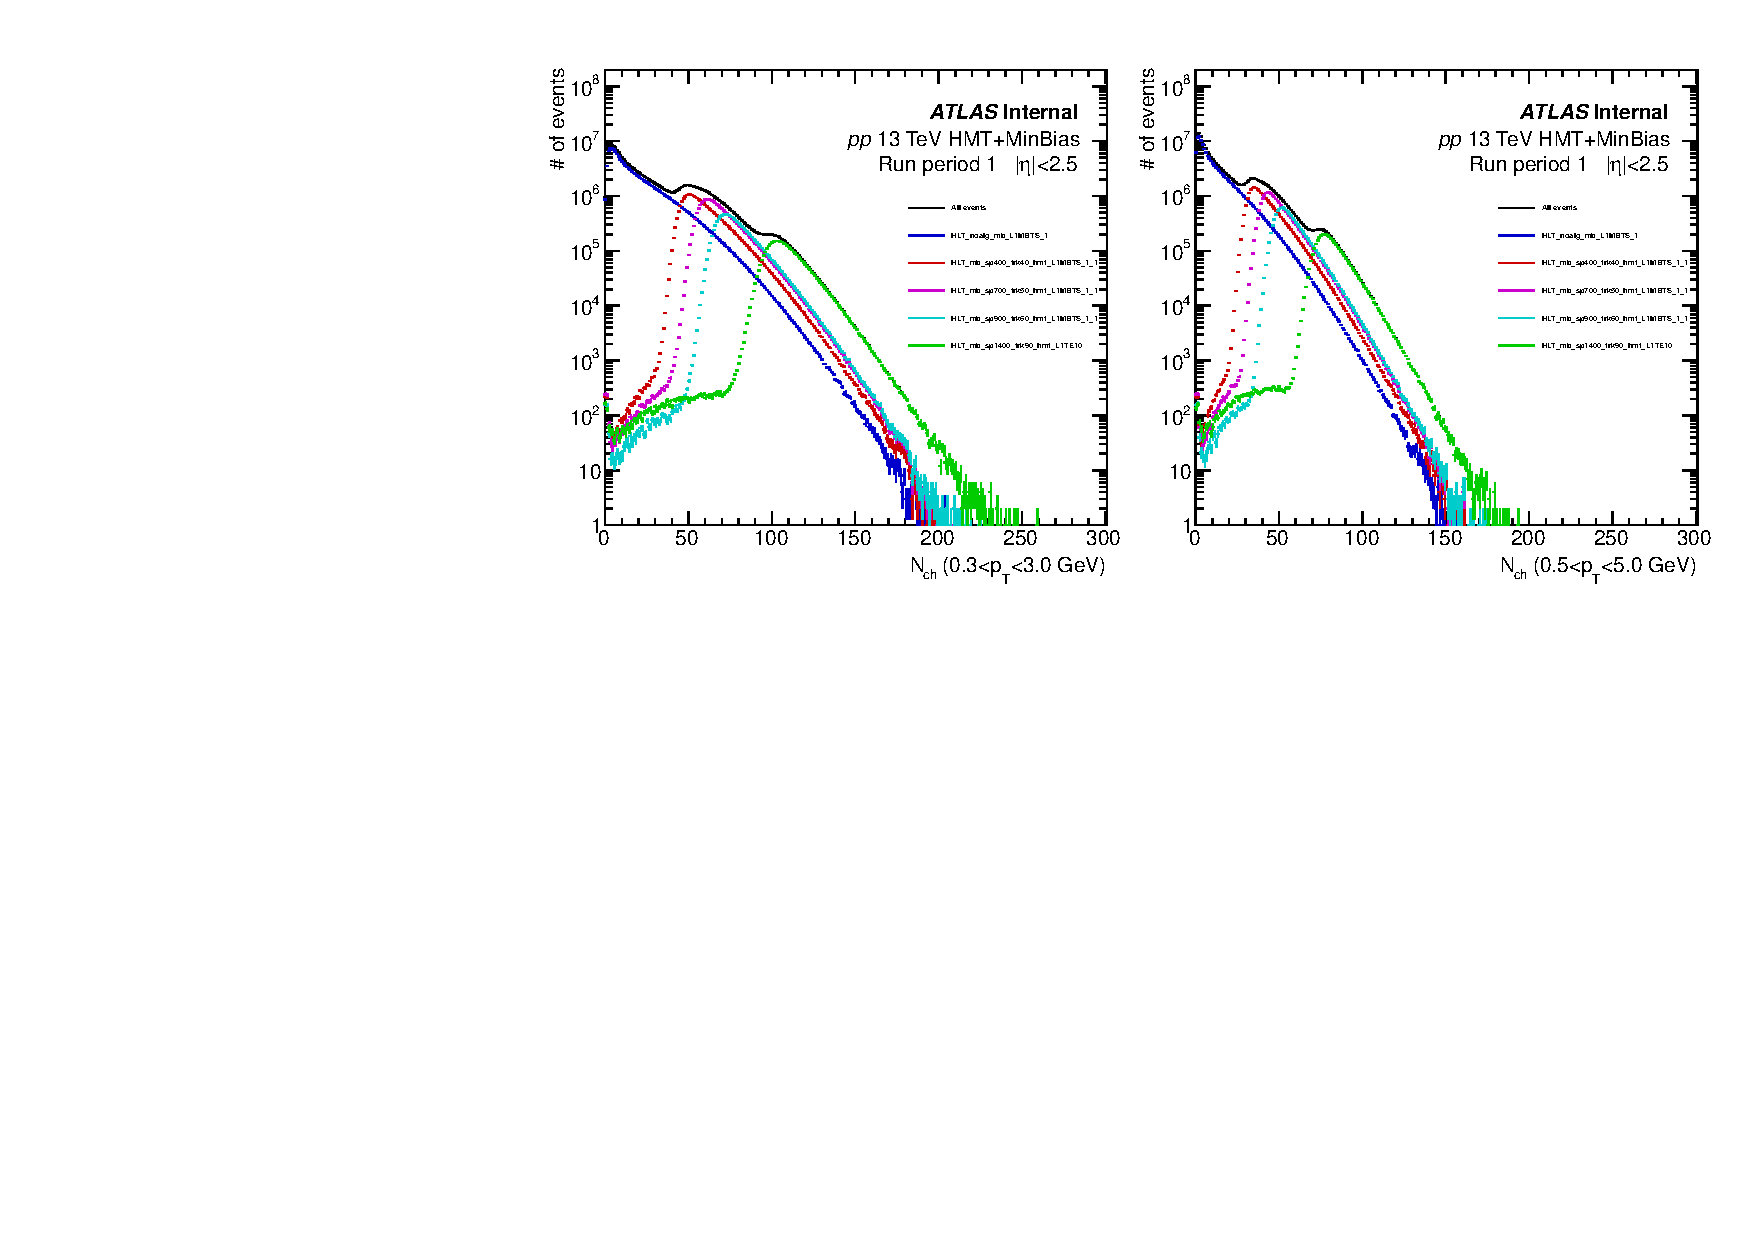
\includegraphics[width=.9\linewidth]{figs/sec_evtSlc/trkDis_pp13_run1.pdf}
\caption{Distribution of number of tracks with two $p_{T}$ thresholds: $0.3<p_{T}<3.0$ GeV and $0.5<p_{T}<5.0$ GeV, in 13 TeV $pp$ run period 1. The major MinBias and HMT triggers are plotted separately. "All events" means all the MinBias and HMT triggers included, mainly from L1TE and HMT performance triggers.}
\label{fig:trkDis_pp13_run1}
\end{figure}

As a summary of total statistics with all runs combined, Fig.\ref{fig:trkDis_pp13_run1} shows the distributions of number of tracks with two $p_{T}$ cuts used in this analysis: $0.3<p_{T}<3.0$ GeV and $0.5<p_{T}<5.0$ GeV. In each case, events collected with different MinBias and HMT triggers are shown separately, since in the end we will apply lower $N_{ch}$ cuts to reduce the selection bias introduced by HMT triggers. Statistics of all the triggers in the MinBias stream (including those triggers not used in this analysis) are listed in the Appendix.

\begin{figure}[H]
\centering
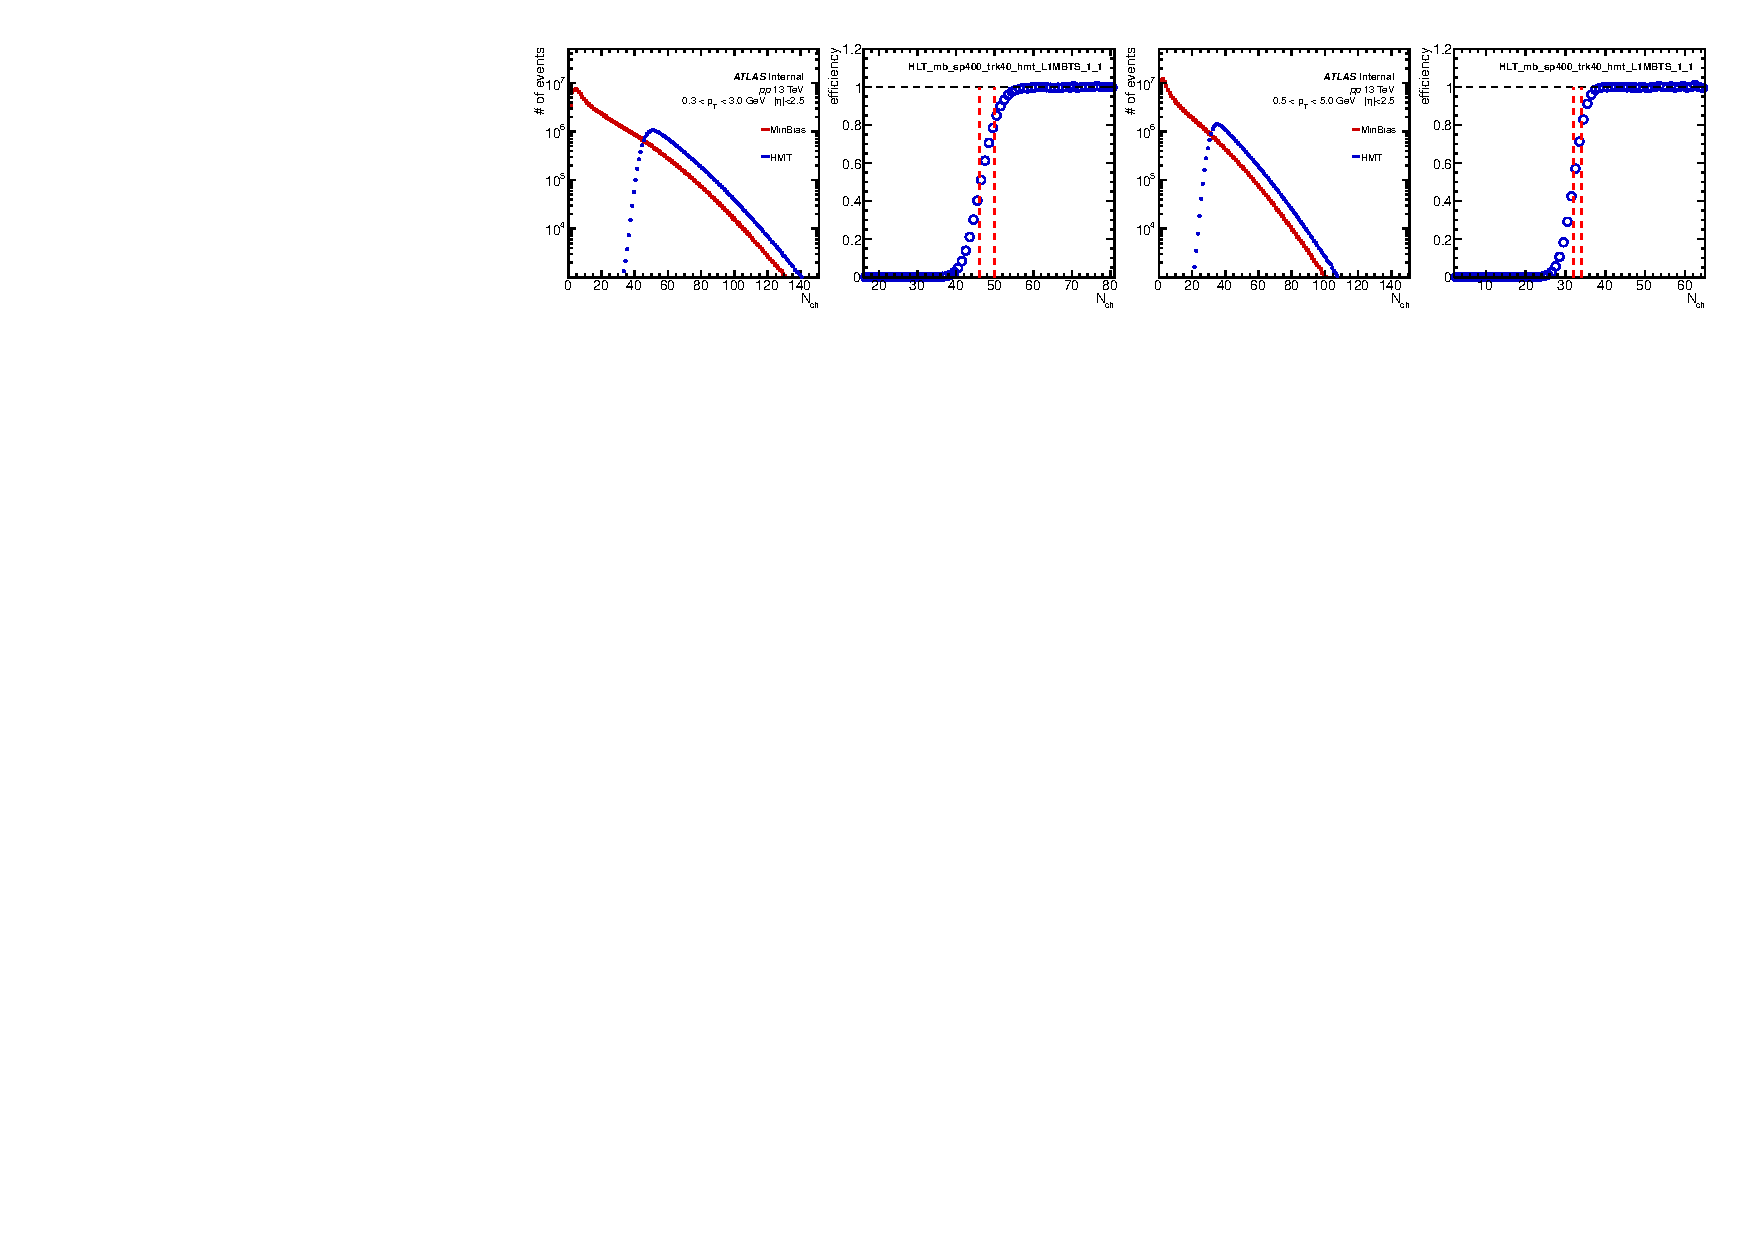
\includegraphics[width=1.\linewidth]{figs/sec_evtSlc/trigEff_pp13_run1/trigEff_Trig11.pdf}
\end{figure}
\begin{figure}[H]
\centering
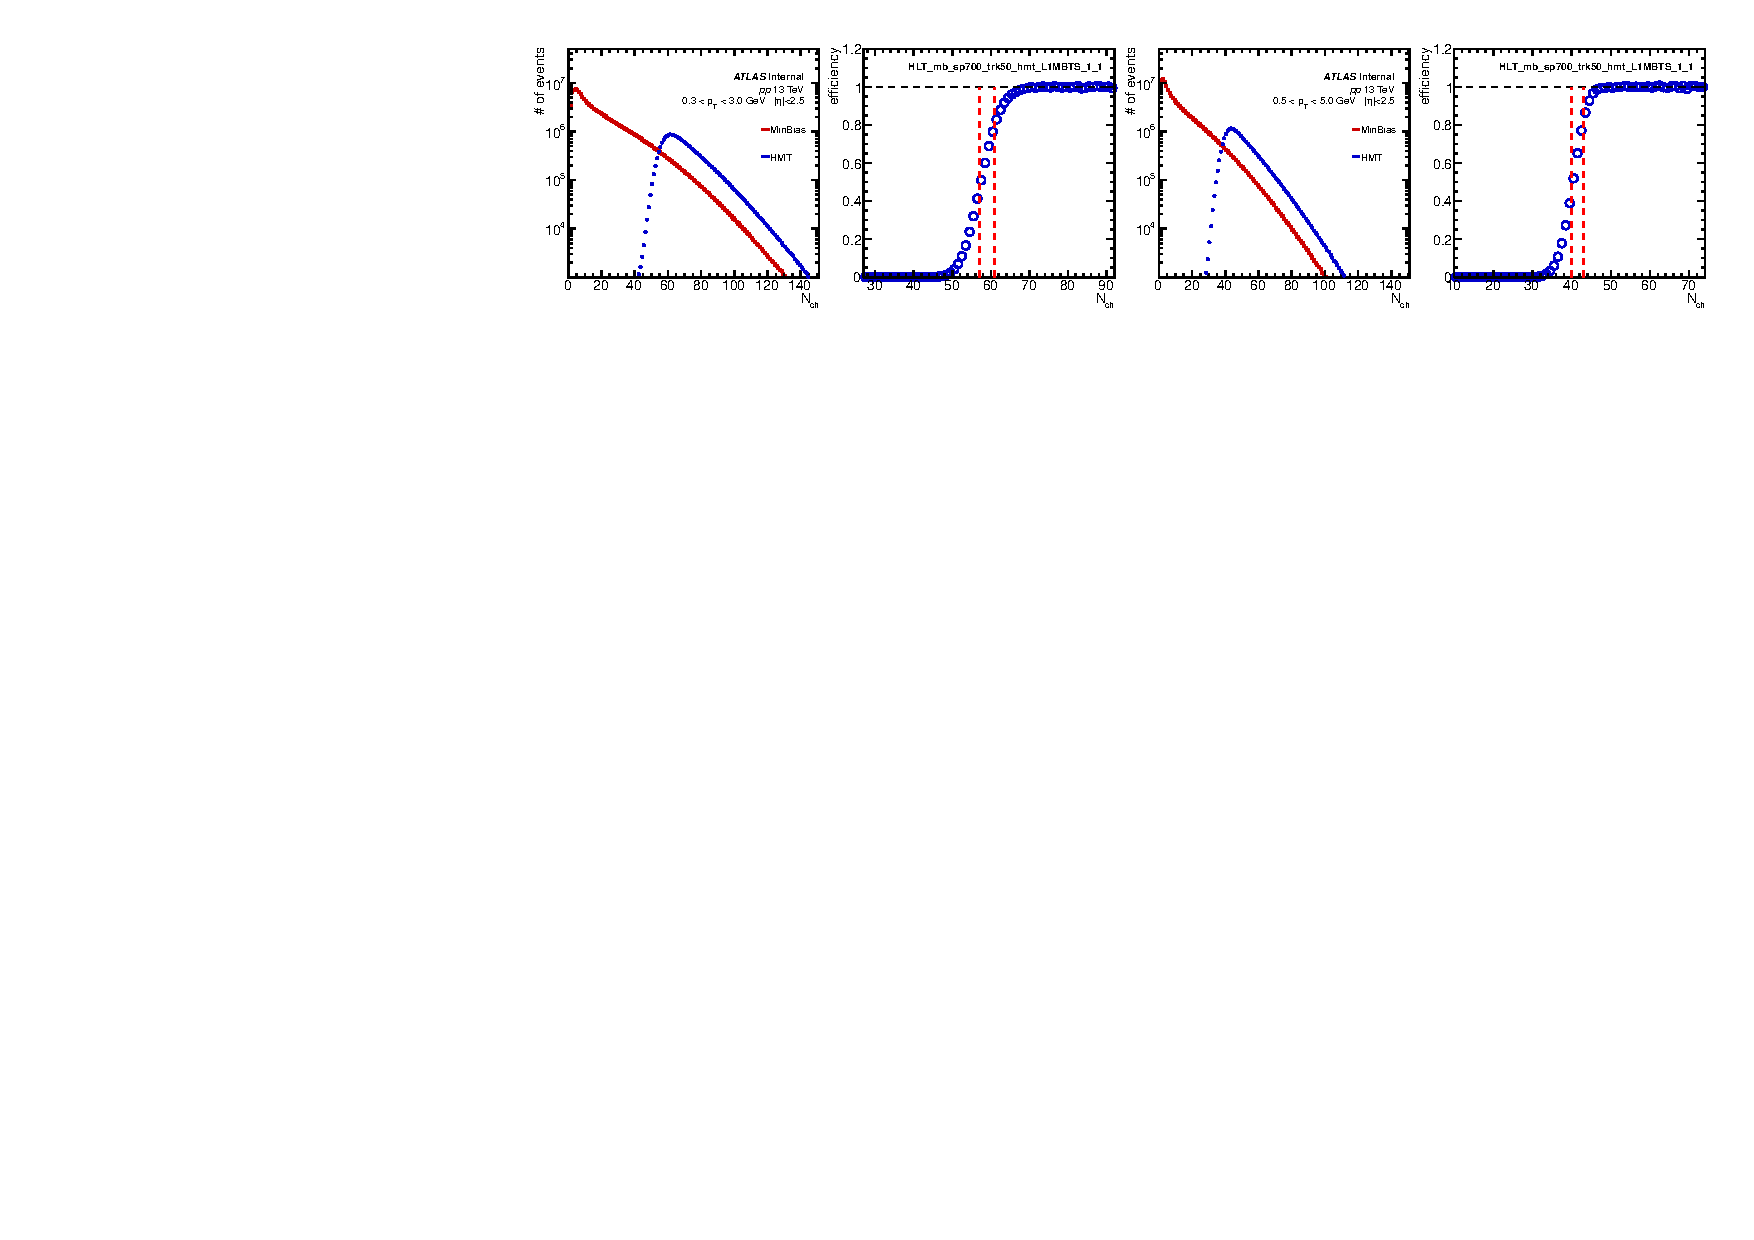
\includegraphics[width=1.\linewidth]{figs/sec_evtSlc/trigEff_pp13_run1/trigEff_Trig12.pdf}
\end{figure}
\begin{figure}[H]
\centering
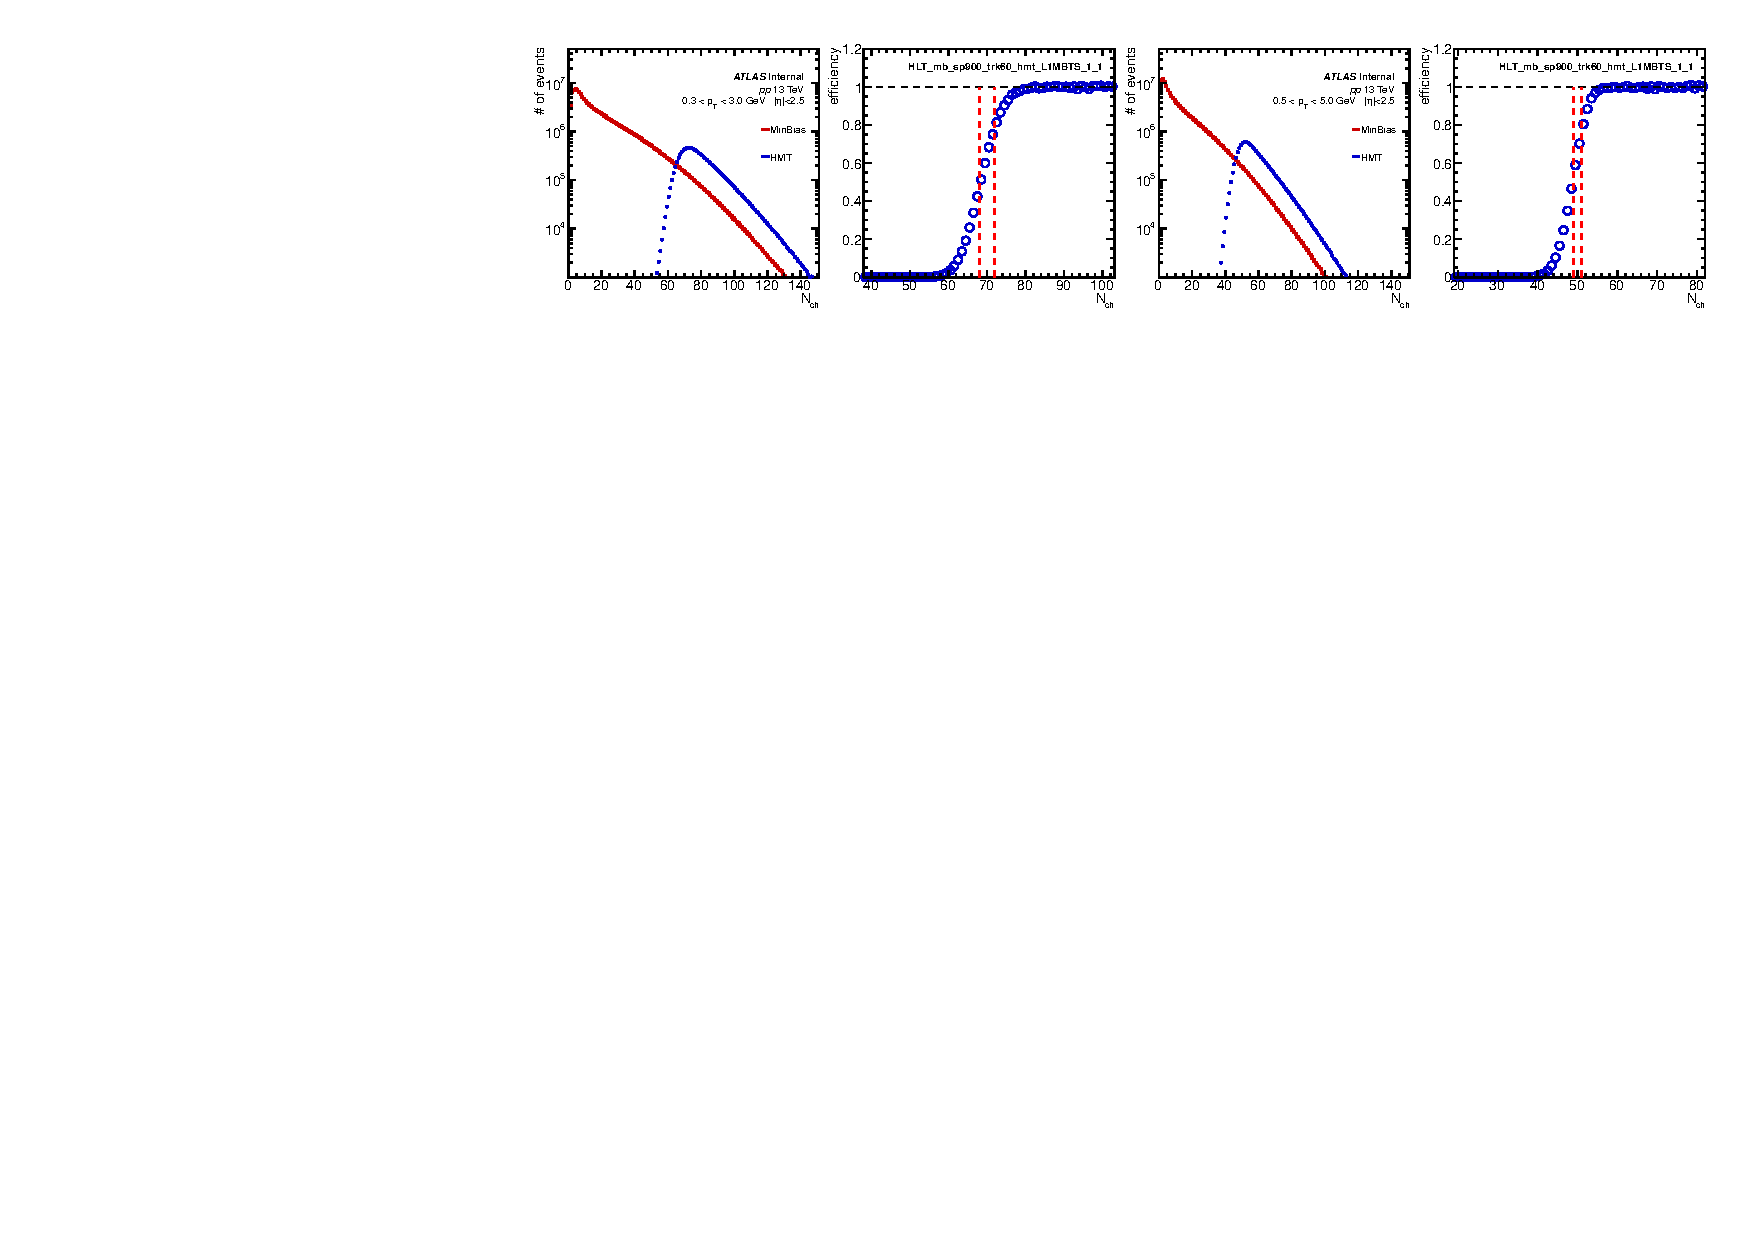
\includegraphics[width=1.\linewidth]{figs/sec_evtSlc/trigEff_pp13_run1/trigEff_Trig13.pdf}
\end{figure}
\begin{figure}[H]
\centering
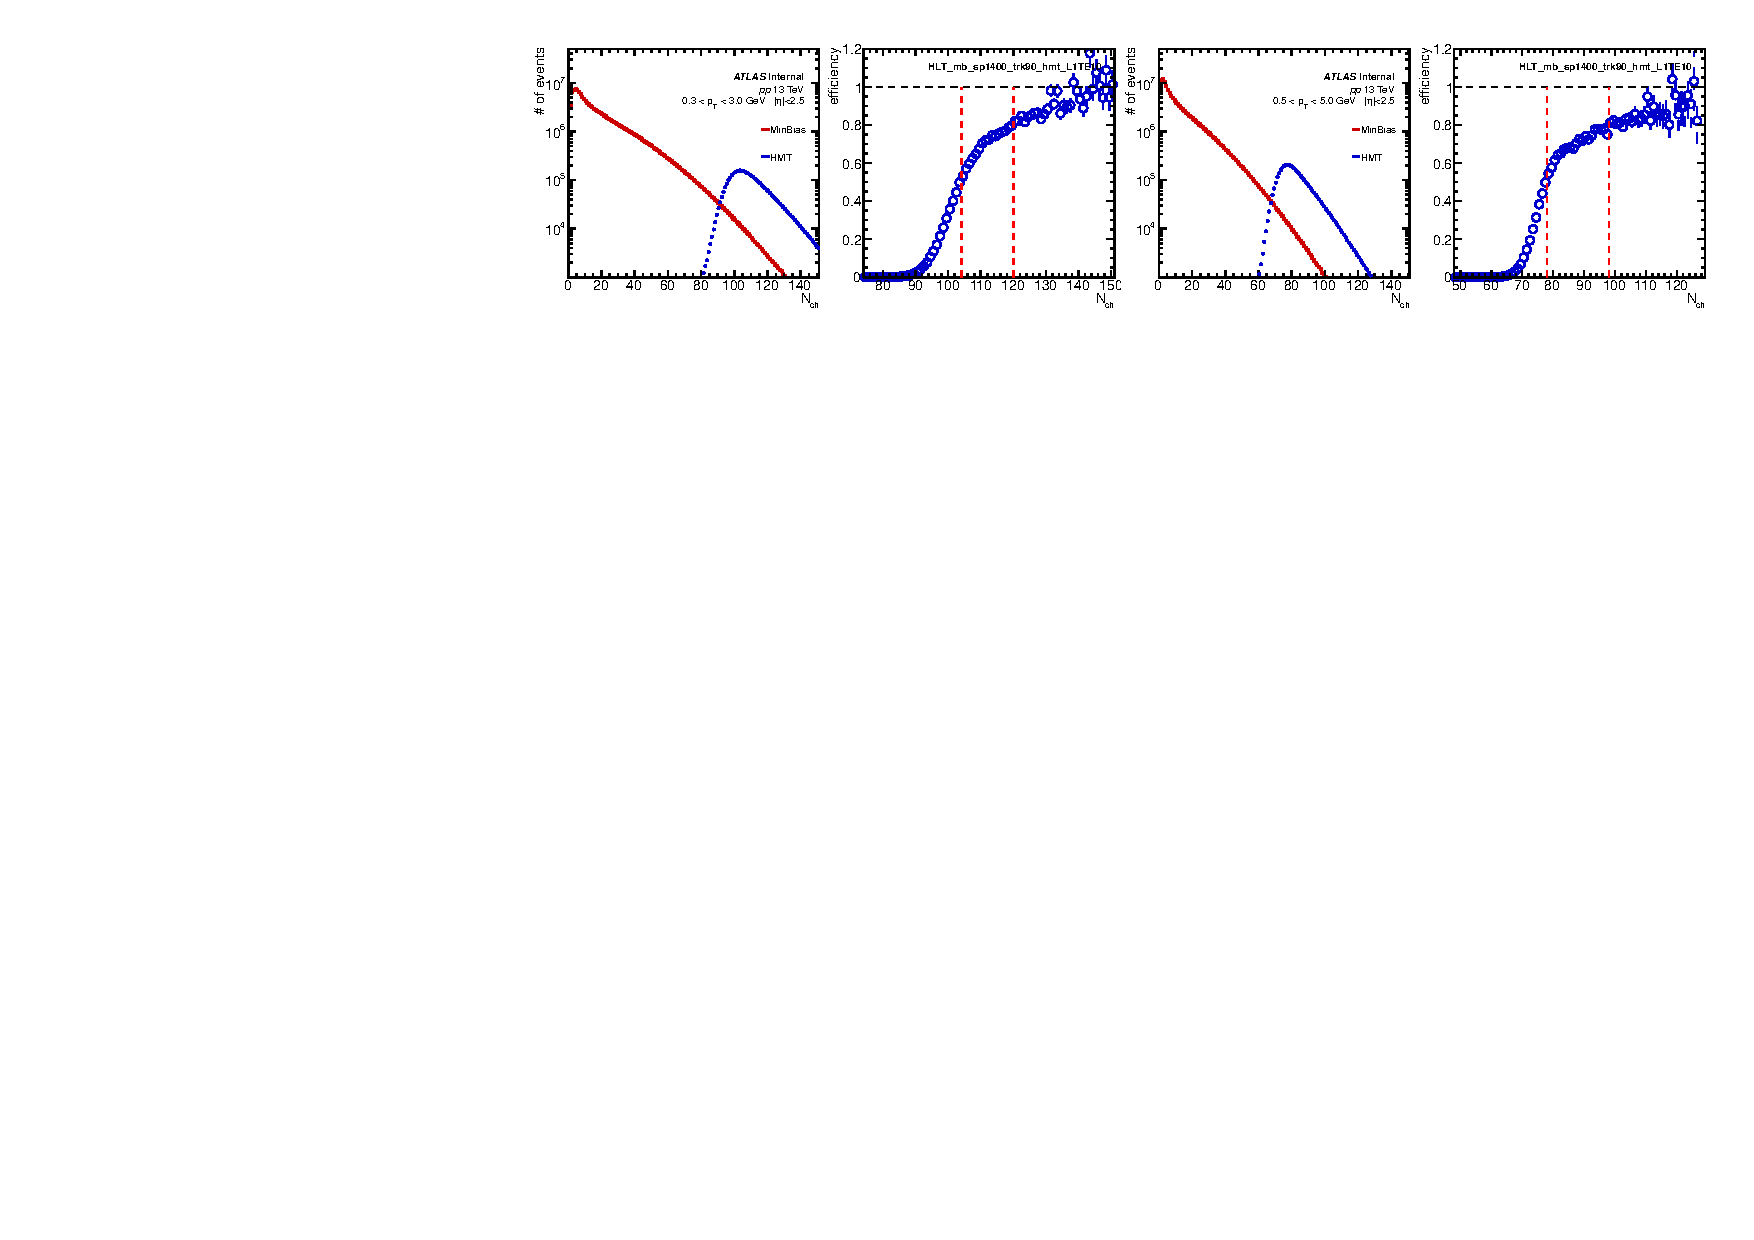
\includegraphics[width=1.\linewidth]{figs/sec_evtSlc/trigEff_pp13_run1/trigEff_Trig15.pdf}
\caption{Trigger efficiencies of all major HMT triggers as a function of number of tracks in two $p_{T}$ ranges: $0.3<p_{T}<3.0$ GeV and $0.5<p_{T}<5.0$ GeV, from 13 TeV $pp$ run period 1. Efficiency is calculated relative to the corresponding MinBias trigger in this run period then scaled to 1.0 in the large $N_{ch}$ region. The two red dash lines indicate 50$\%$ and 80$\%$ efficiency cuts.}
\label{fig:trigEff_pp13_run1}
\end{figure}
During the data taking, both minbias and HMT triggers are prescaled. The triggers efficiency $\epsilon$ is estimated on the statistical level:
\begin{equation}
\epsilon^{\text{HMT}}\equiv\frac{\text{number of events passed HMT trigger}*\text{PS of HMT trigger}}{\text{number of events passed MB trigger}*\text{PS of MB trigger}}
\end{equation}
Since the number of events with high $N_{ch}$ triggered by minbias trigger is limited (during some runs the prescale of minbias triggers are very high), the estimated HMT trigger efficiency could fluctuate around $1$ in some cases. However, because the turn-on of HMT trigger is very sharp, $N_{ch}$ cut with $50\%$ and $80\%$ efficiency are not affected by this estimation. Trigger efficiencies of all the major HMT triggers are summarized in Fig.~\ref{fig:trigEff_pp13_run1}, where efficiencies are shown for two $p_{T}$ ranges separately: $0.3<p_{T}<3.0$ GeV and $0.5<p_{T}<5.0$ GeV. In order to remove the potential bias introduced by trigger selections, HMT events are only used when their corresponding trigger efficiency is larger than 50$\%$. Another criteria of larger than 80$\%$ is applied as a cross check and will be included as one of the systematics.



\subsubsection{Run period 2}
The 2nd run period data was taken in 2016 and there are 2 runs used for this analysis:
\begin{itemize}

\item Run 299390, peak $\mu=0.052$, 4.1 million events
\begin{itemize}[leftmargin=*]
\item[] \verb|data16_13TeV.00299390.physics_MinBias.recon.AOD.r8358/|
\end{itemize}

\item Run 300287, peak $\mu=0.052$, 8.1 million events
\begin{itemize}[leftmargin=*]
\item[] \verb|data16_13TeV.00300287.physics_MinBias.recon.AOD.r8358/|
\end{itemize}

\end{itemize}
The major MinBias and HMT triggers applied in this run period are:
\begin{itemize}
\item \verb|HLT_noalg_mb_L1MBTS_1_1|
\item \verb|HLT_mb_sp1800_hmtperf_L1TE5|
\item \verb|HLT_mb_sp1500_hmtperf_L1TE10|
\item \verb|HLT_mb_sp900_trk60_hmt_L1MBTS_1_1|
\item \verb|HLT_mb_sp1000_trk70_hmt_L1TE5|
\item \verb|HLT_mb_sp1400_trk90_hmt_L1TE10|
\end{itemize}
where there is one new trigger item:
\begin{itemize}
\item \verb|hmt_perf|: performance triggers of HMT, usually without online track cuts;
\end{itemize}

\begin{figure}[H]
\centering
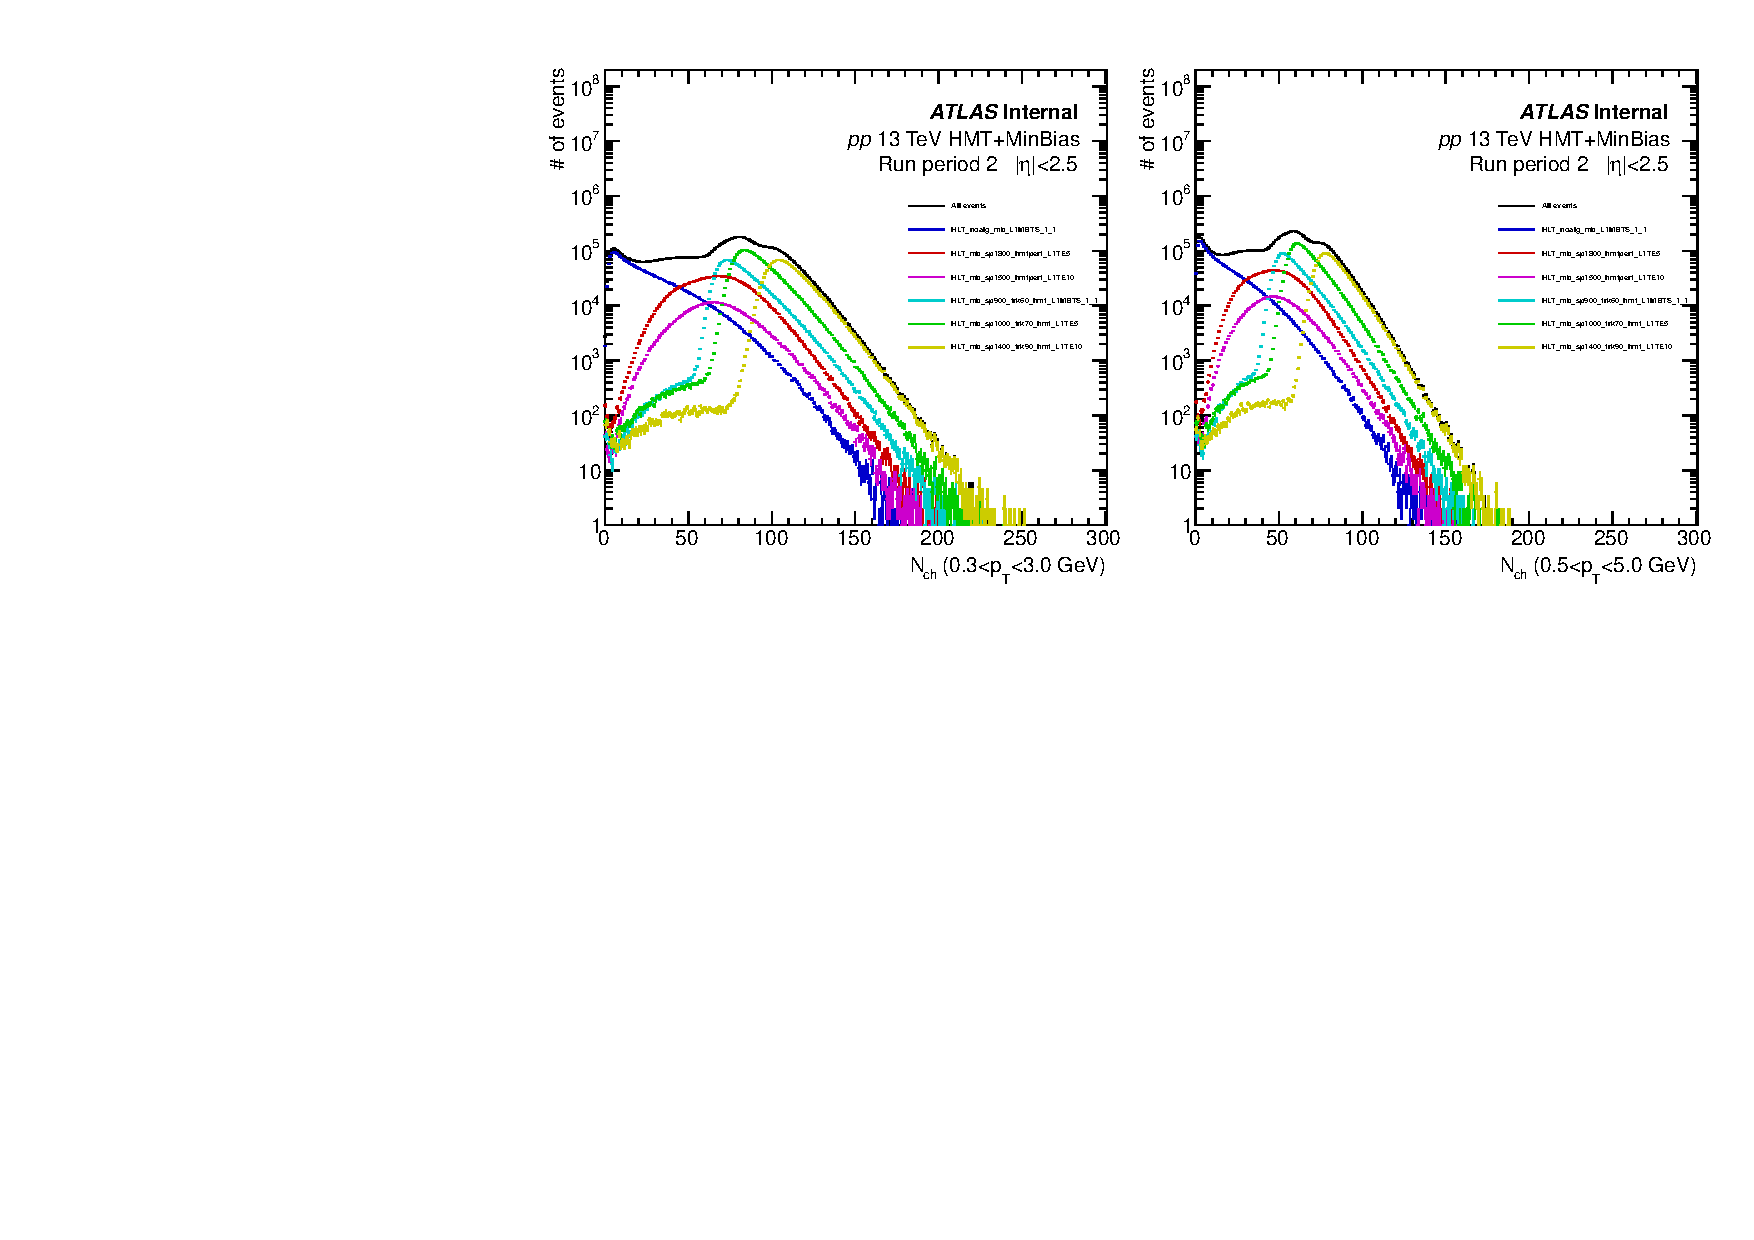
\includegraphics[width=.9\linewidth]{figs/sec_evtSlc/trkDis_pp13_run2.pdf}
\caption{Distribution of number of tracks with two $p_{T}$ thresholds: $0.3<p_{T}<3.0$ GeV and $0.5<p_{T}<5.0$ GeV, in 13 TeV $pp$ run period 2. The major MinBias and HMT triggers are plotted separately.}
\label{fig:trkDis_pp13_run2}
\end{figure}
The summary of statistics with all the major triggers used in this analysis are shown in Fig.~\ref{fig:trkDis_pp13_run2}.

\begin{figure}[H]
\centering
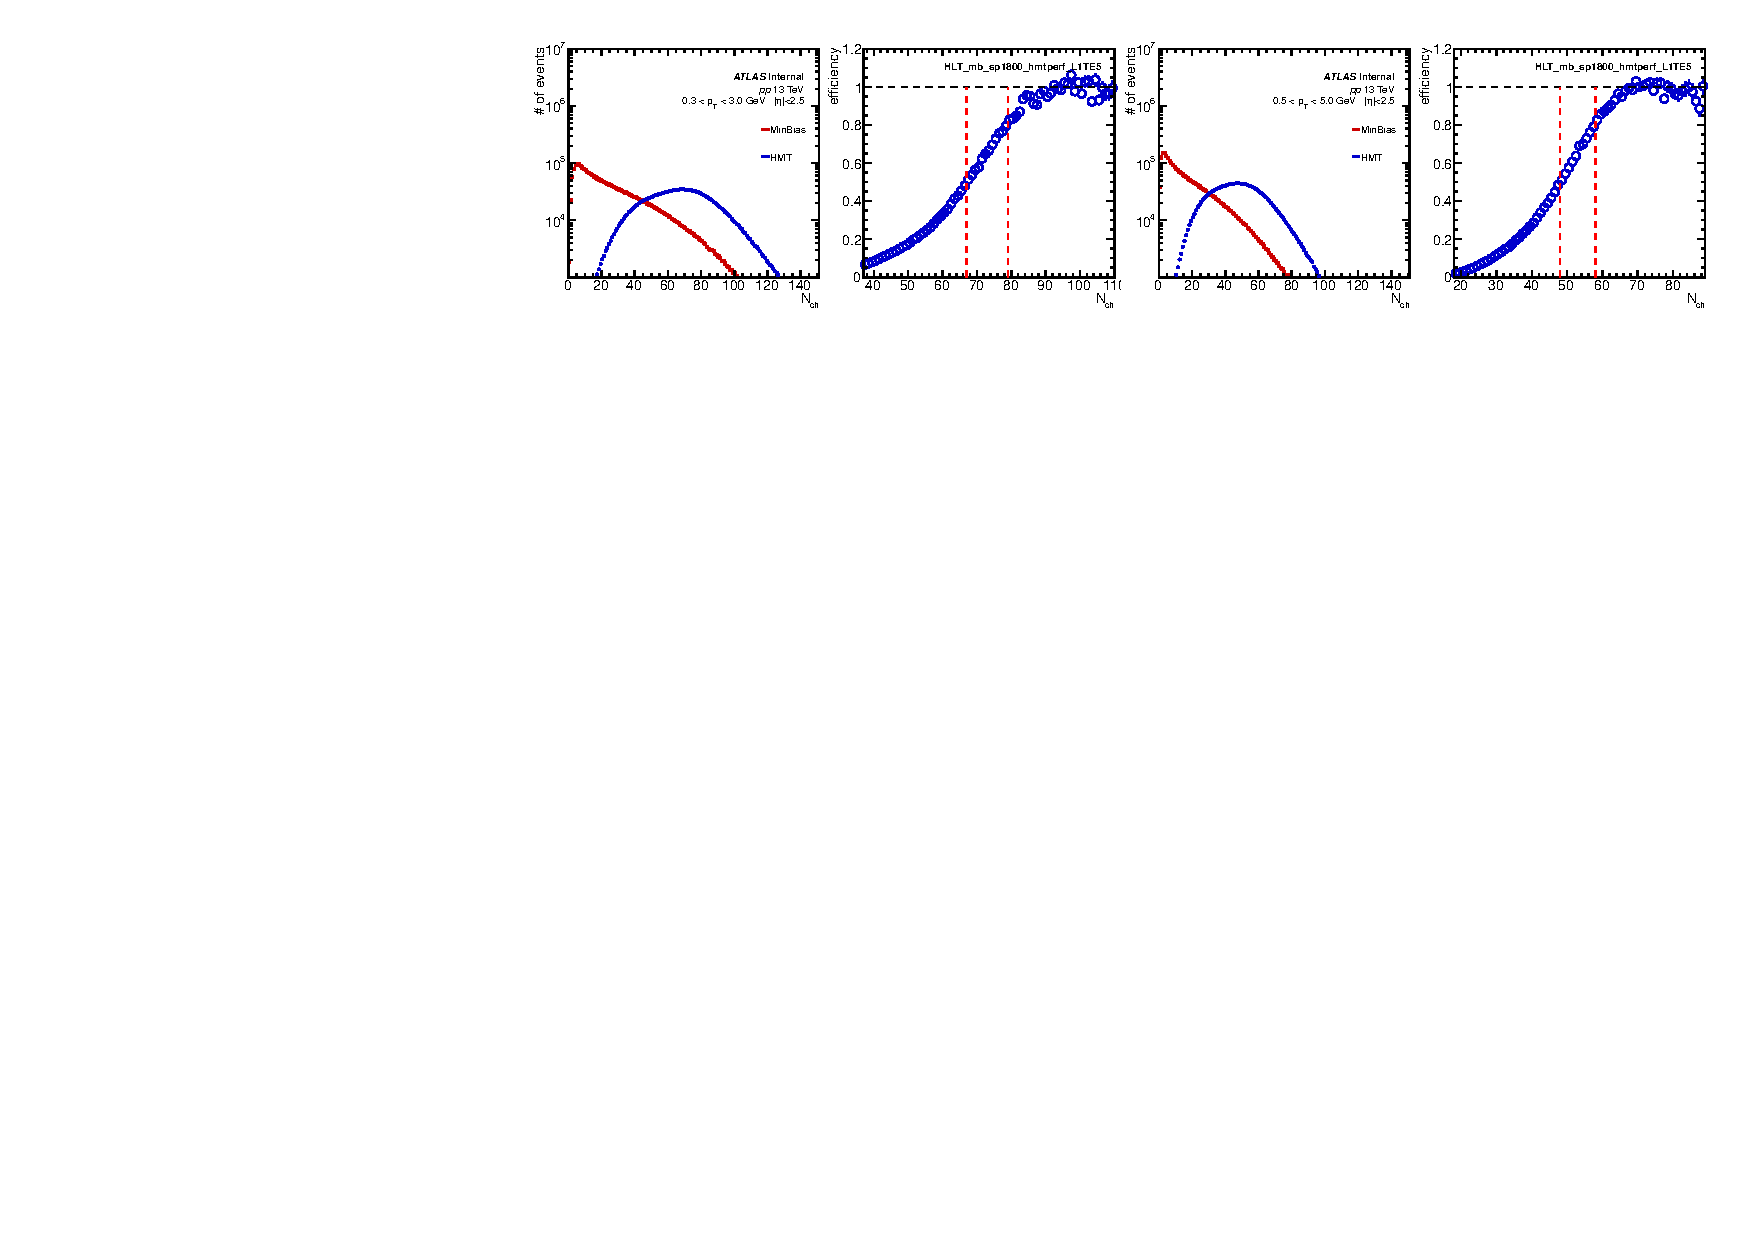
\includegraphics[width=1.\linewidth]{figs/sec_evtSlc/trigEff_pp13_run2/trigEff_Trig17.pdf}
\end{figure}
\begin{figure}[H]
\centering
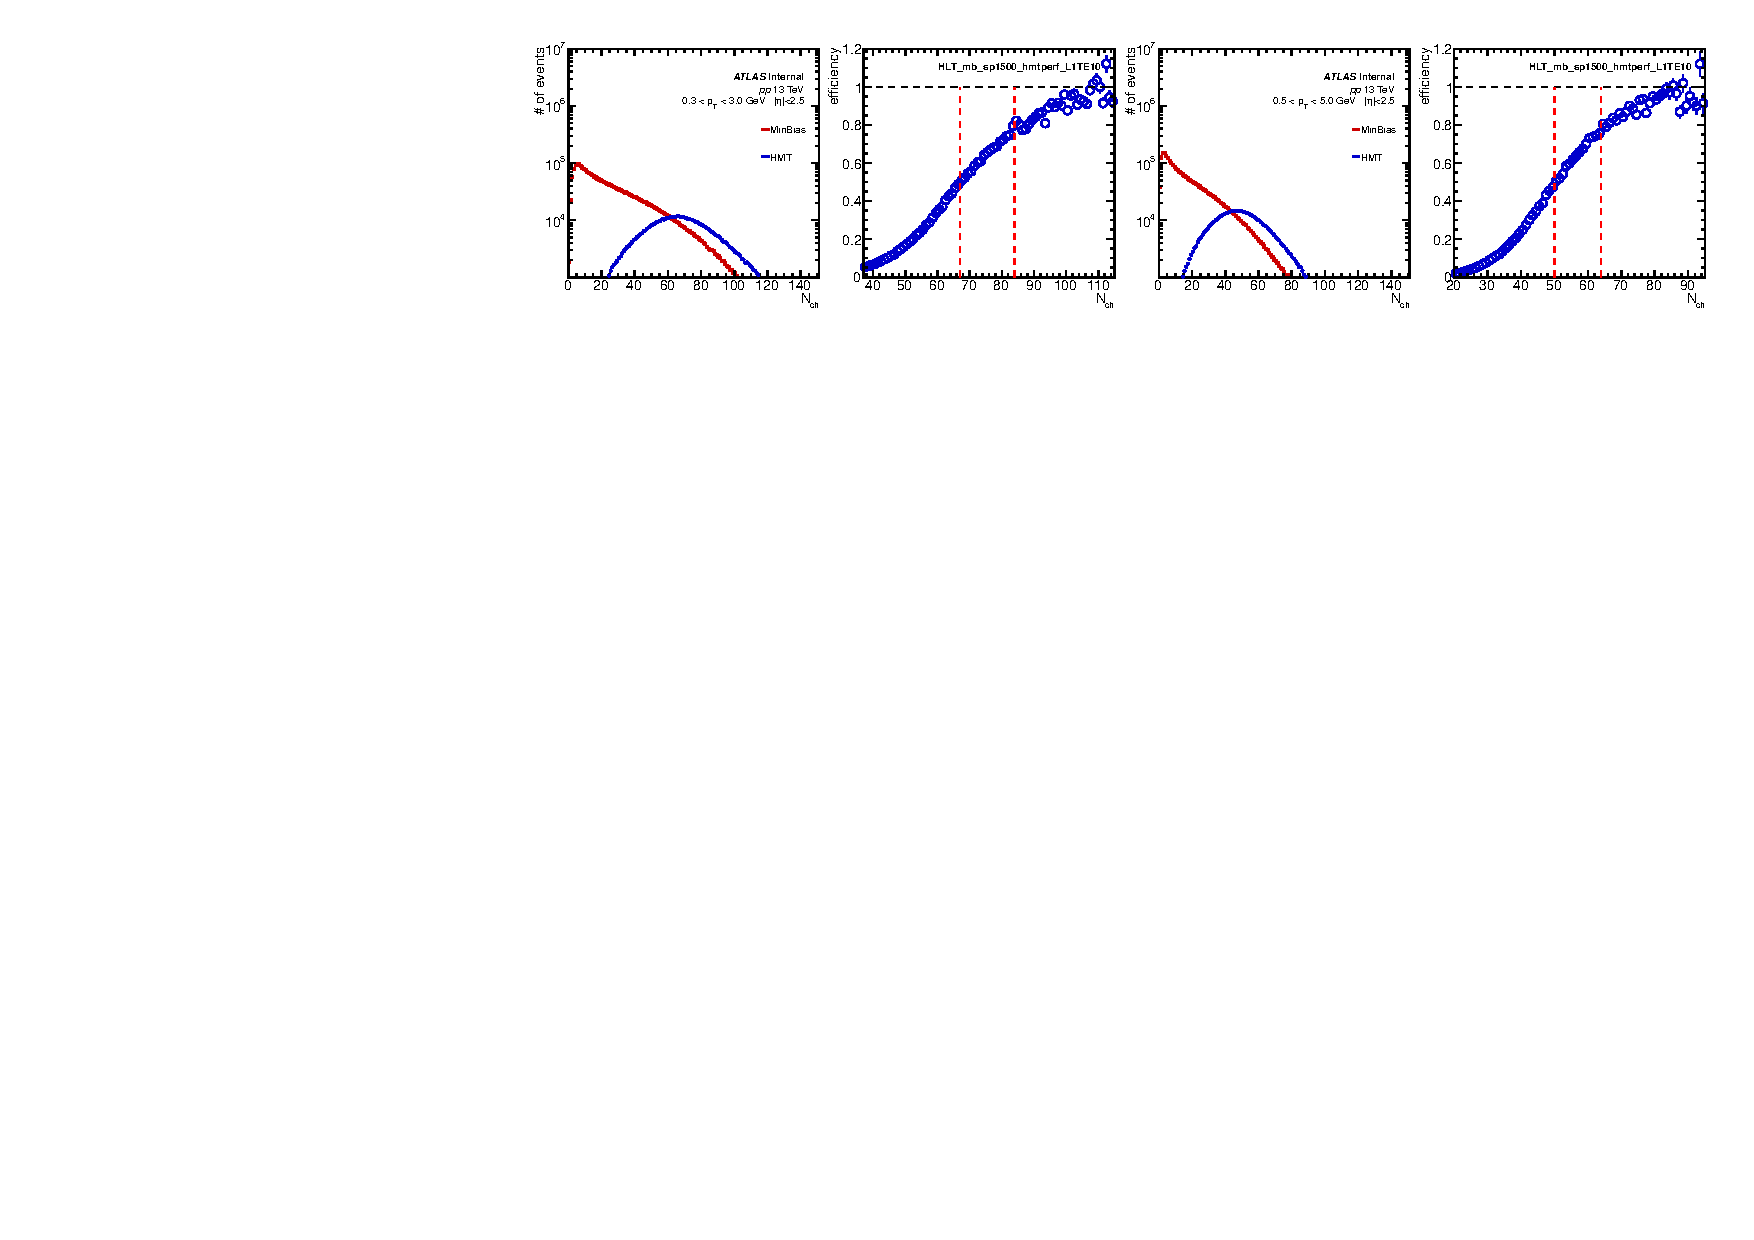
\includegraphics[width=1.\linewidth]{figs/sec_evtSlc/trigEff_pp13_run2/trigEff_Trig18.pdf}
\end{figure}
\begin{figure}[H]
\centering
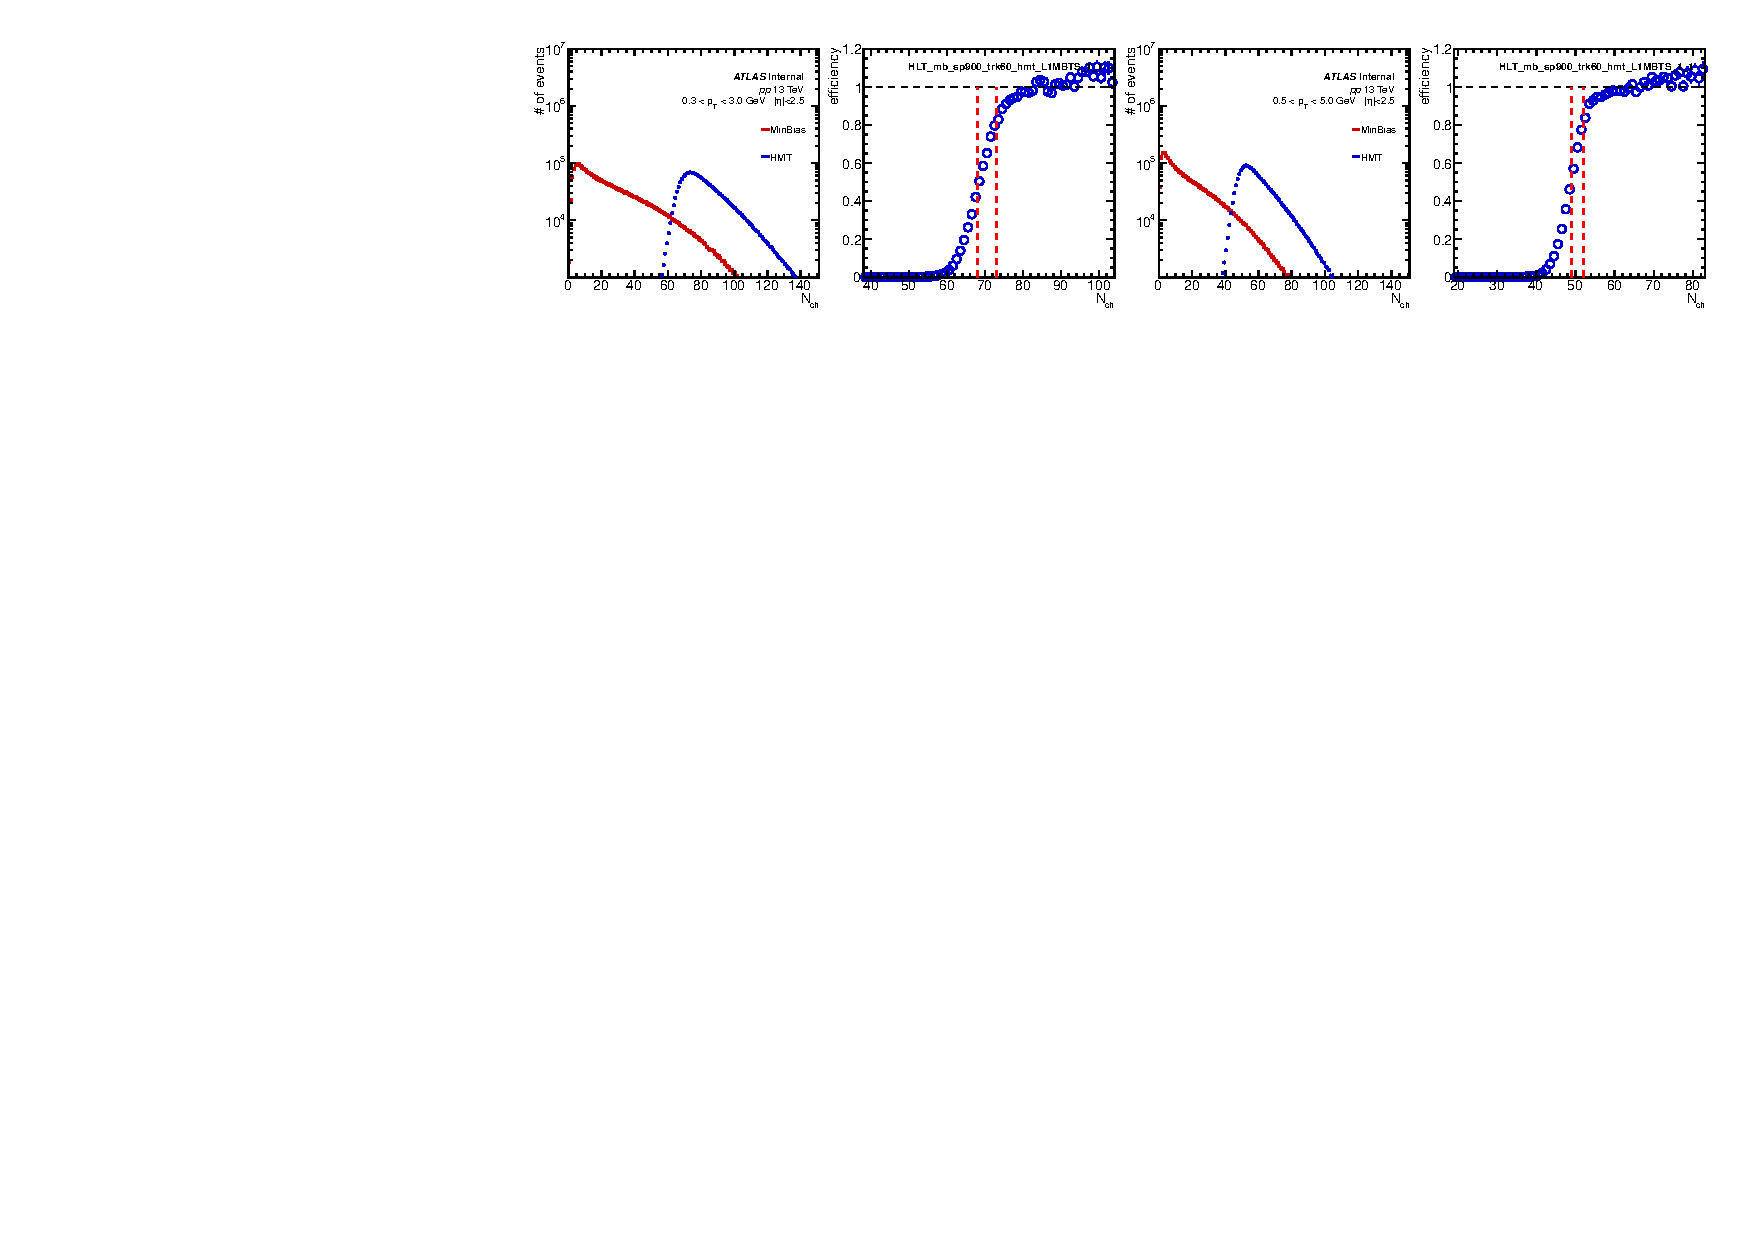
\includegraphics[width=1.\linewidth]{figs/sec_evtSlc/trigEff_pp13_run2/trigEff_Trig19.pdf}
\end{figure}
\begin{figure}[H]
\centering
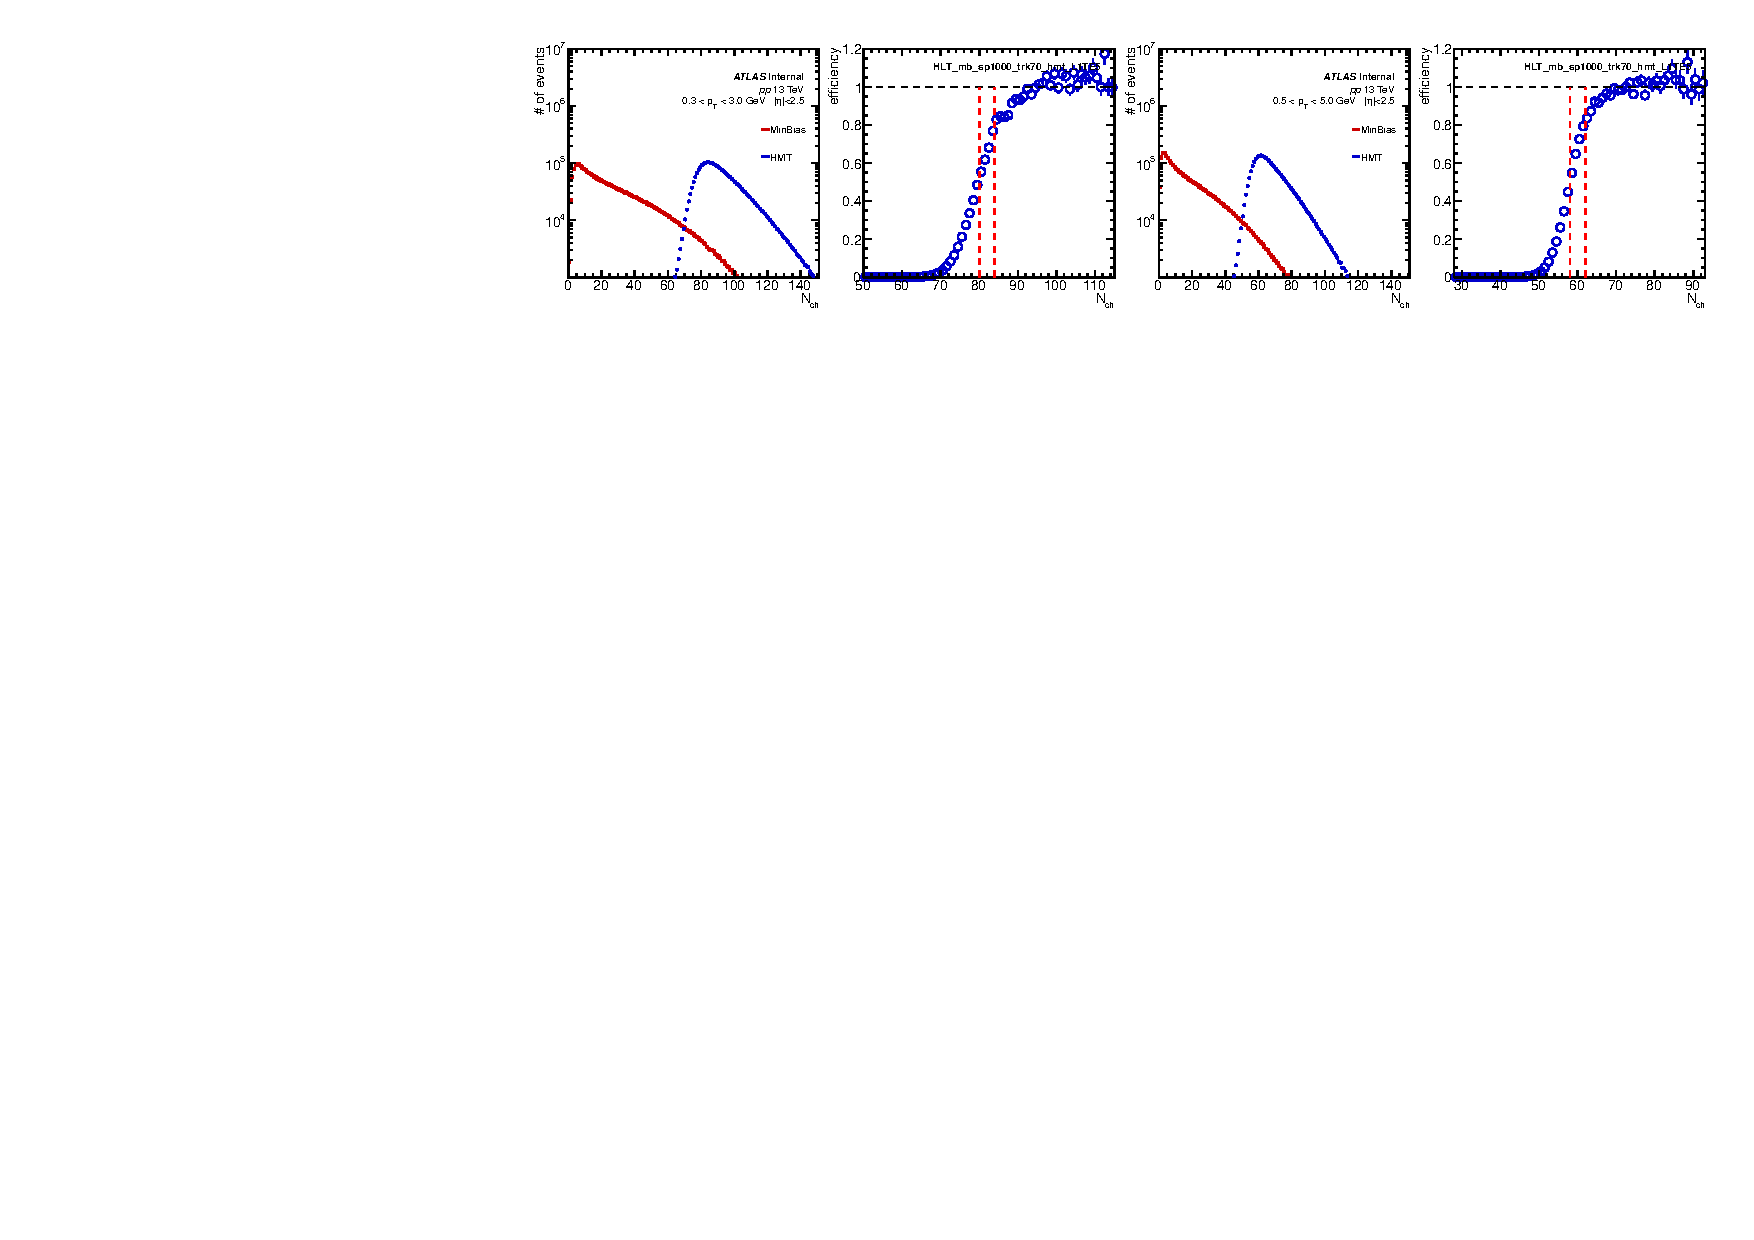
\includegraphics[width=1.\linewidth]{figs/sec_evtSlc/trigEff_pp13_run2/trigEff_Trig22.pdf}
\end{figure}
\begin{figure}[H]
\centering
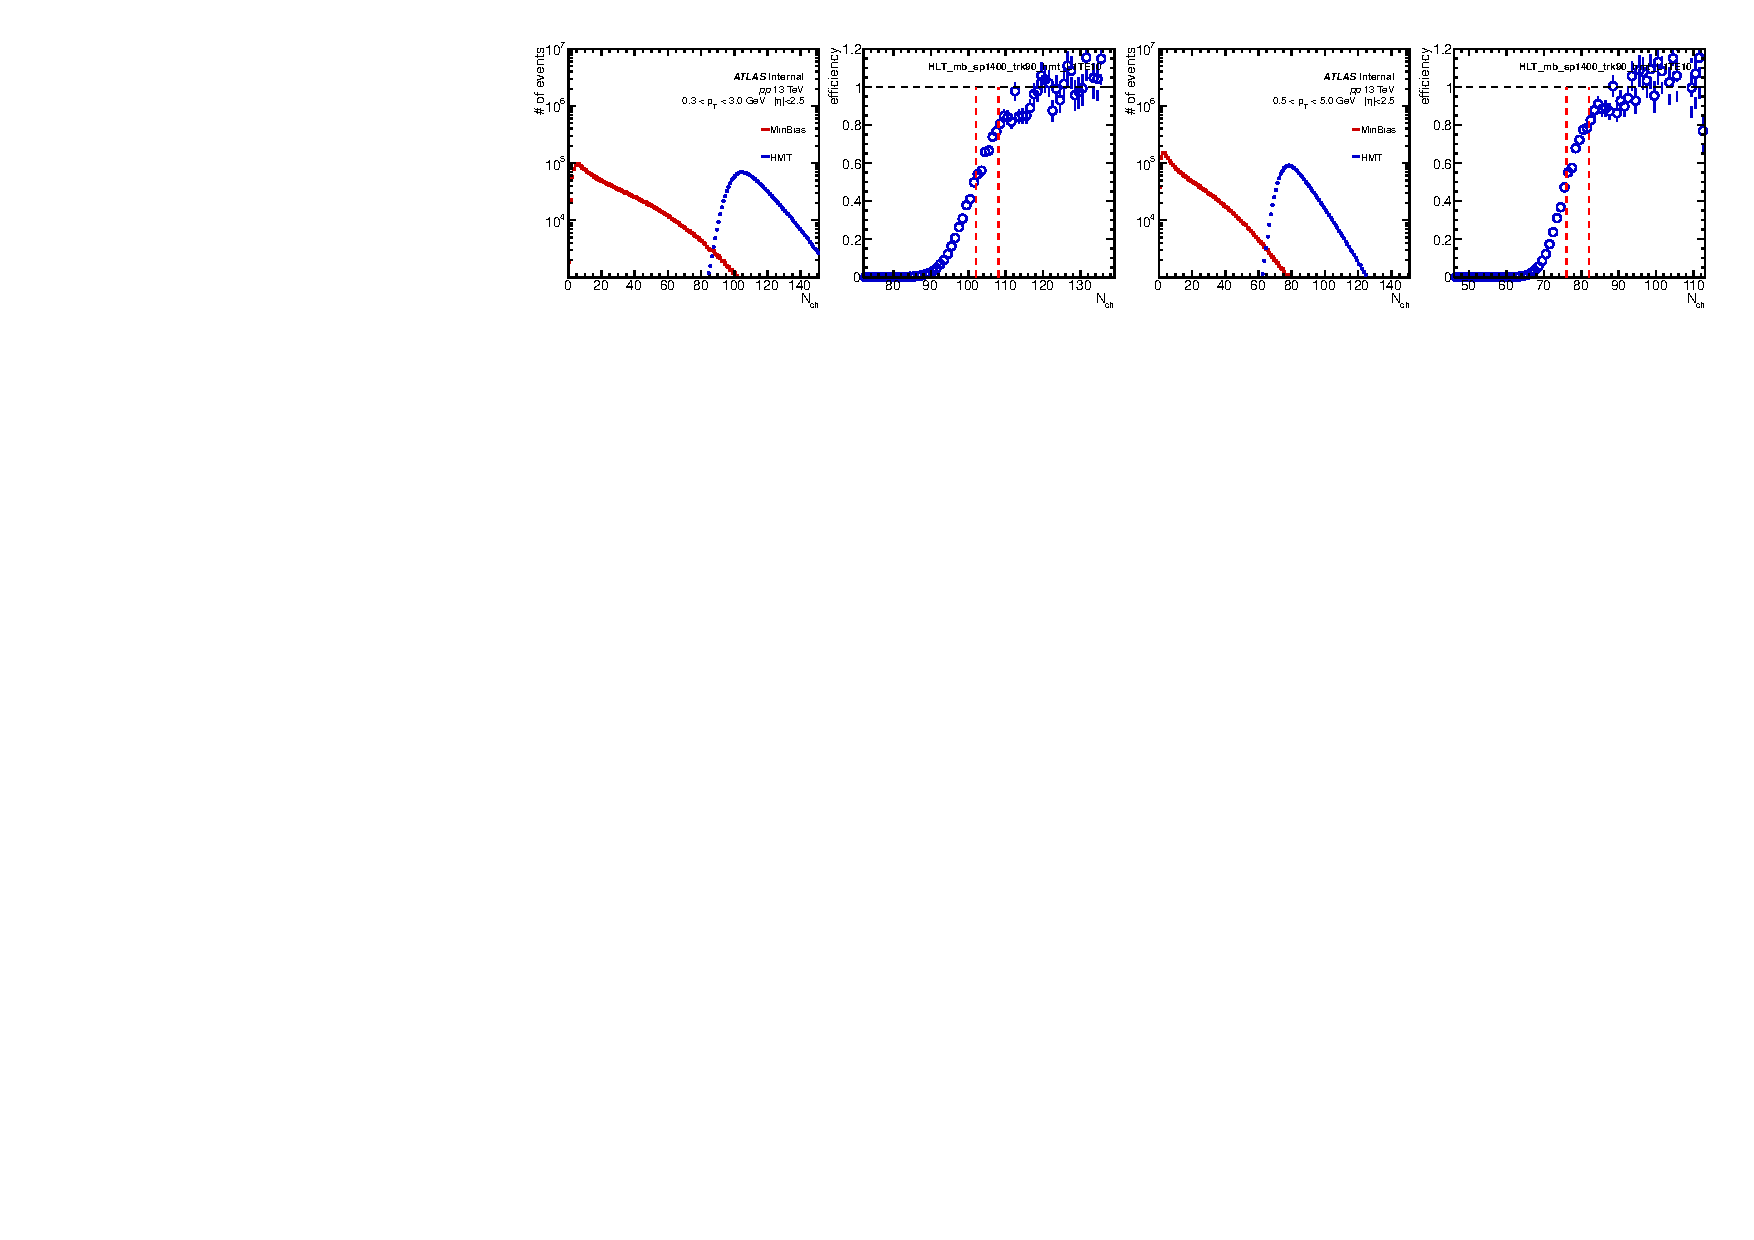
\includegraphics[width=1.\linewidth]{figs/sec_evtSlc/trigEff_pp13_run2/trigEff_Trig24.pdf}
\caption{Trigger efficiencies of all major HMT triggers as a function of number of tracks in two $p_{T}$ ranges: $0.3<p_{T}<3.0$ GeV and $0.5<p_{T}<5.0$ GeV, from 13 TeV $pp$ run period 2. Efficiency is calculated relative to the corresponding MinBias trigger in this run period then scaled to 1.0 in the large $N_{ch}$ region. The two red dash lines indicate 50$\%$ and 80$\%$ efficiency cuts.}
\label{fig:trigEff_pp13_run2}
\end{figure}
Trigger efficiencies of all the major HMT triggers are summarized in Fig.~\ref{fig:trigEff_pp13_run2}, where efficiencies are shown for two $p_{T}$ ranges separately: $0.3<p_{T}<3.0$ GeV and $0.5<p_{T}<5.0$ GeV.



\subsubsection{Run period 3}
The 3rd run period data was taken in 2016 and there is one low-$\mu$ run used for this analysis:
\begin{itemize}

\item Run 305359, peak $\mu=0.06$, 16.5 million events
\begin{itemize}[leftmargin=*]
\item[] \verb|data16_13TeV.00305359.physics_MinBias.recon.AOD.r8489/|
\end{itemize}

\end{itemize}
The major MinBias and HMT triggers applied in this run period are:
\begin{itemize}
\item \verb|HLT_mb_mbts_L1MBTS_1_1|
\item \verb|HLT_noalg_mb_L1TE30|
\item \verb|HLT_mb_sp700_hmtperf_L1TE5|
\item \verb|HLT_mb_sp1500_hmtperf_L1TE10|
\item \verb|HLT_mb_sp1000_trk70_hmt_L1TE5|
\item \verb|HLT_mb_sp1400_trk90_hmt_L1TE10|
\end{itemize}

\begin{figure}[H]
\centering
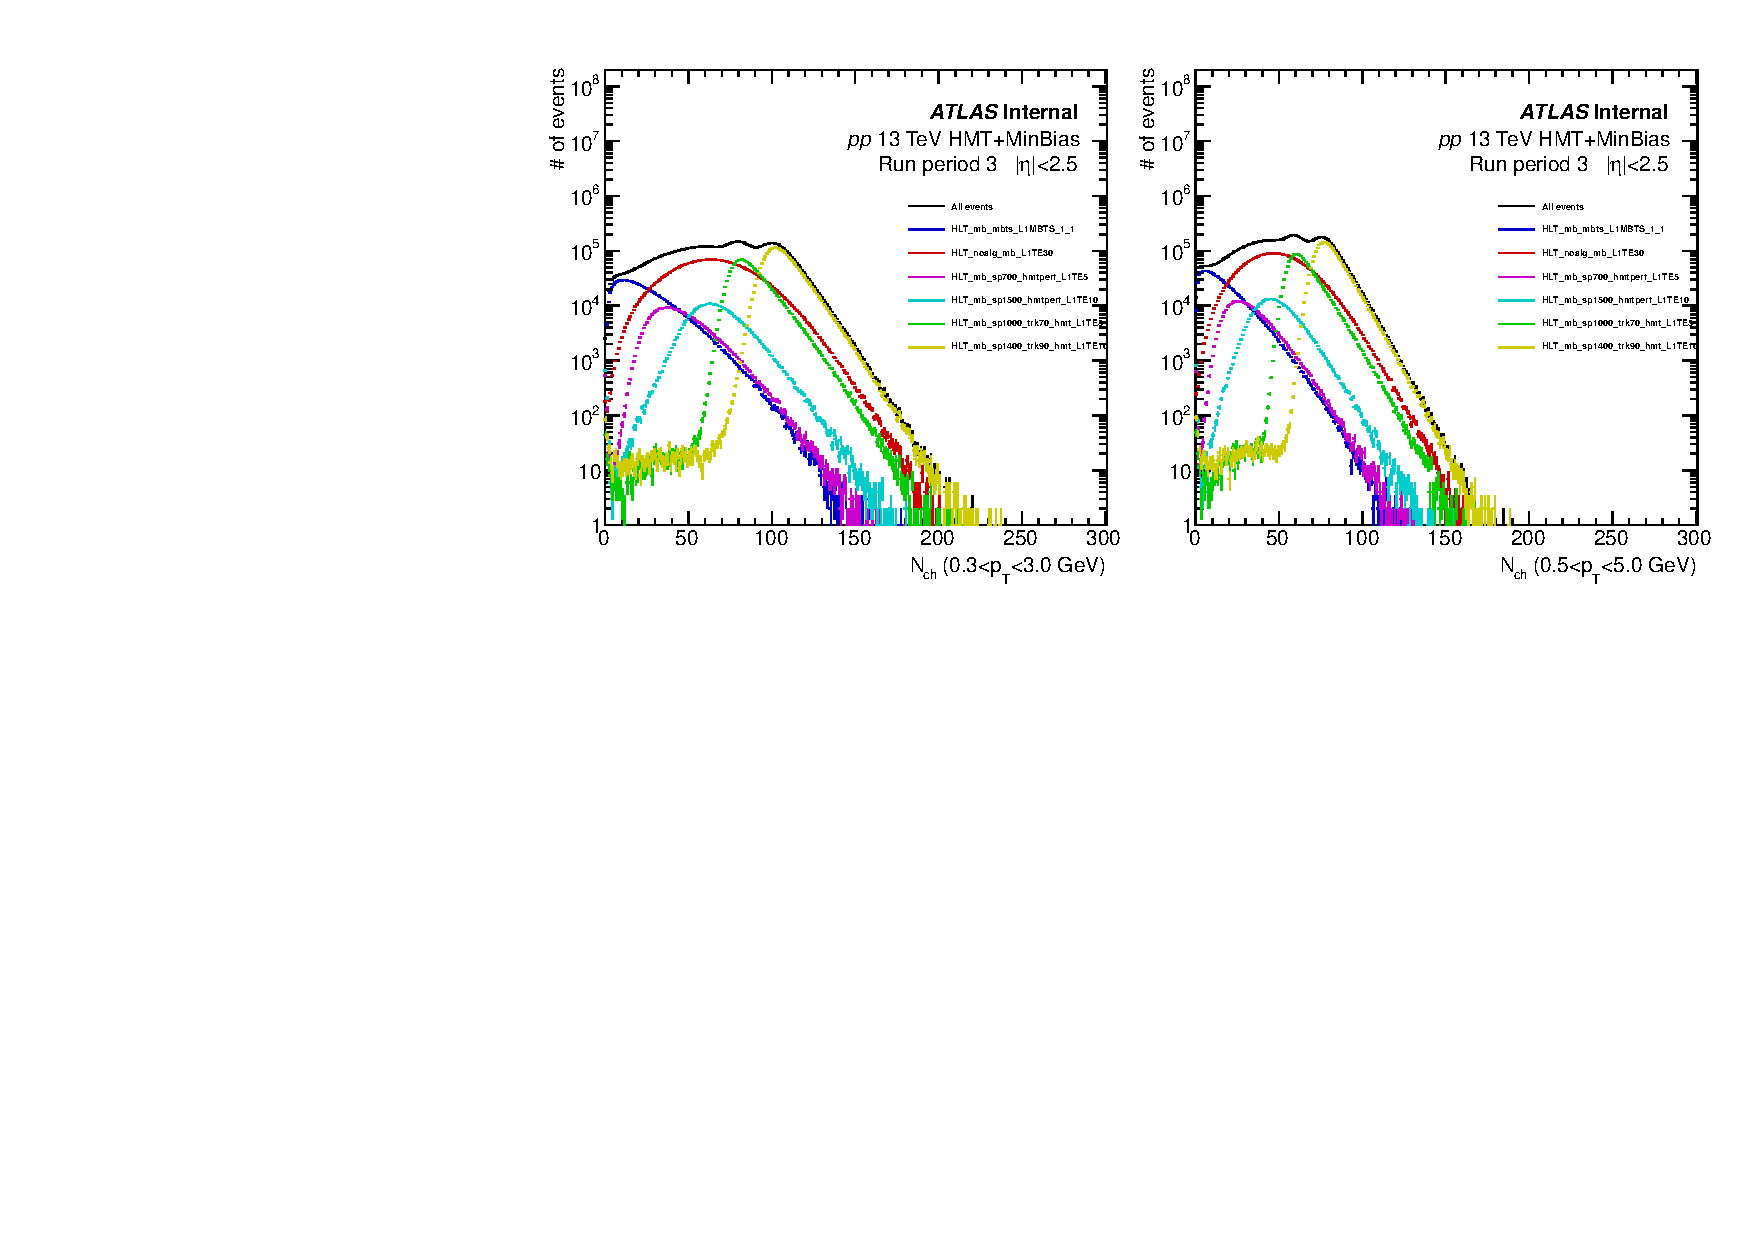
\includegraphics[width=.9\linewidth]{figs/sec_evtSlc/trkDis_pp13_run3.pdf}
\caption{Distribution of number of tracks with two $p_{T}$ thresholds: $0.3<p_{T}<3.0$ GeV and $0.5<p_{T}<5.0$ GeV, in 13 TeV $pp$ run period 3. The major MinBias and HMT triggers are plotted separately.}
\label{fig:trkDis_pp13_run3}
\end{figure}
The summary of statistics with all the major triggers used in this analysis are shown in Fig.~\ref{fig:trkDis_pp13_run3}.

\begin{figure}[H]
\centering
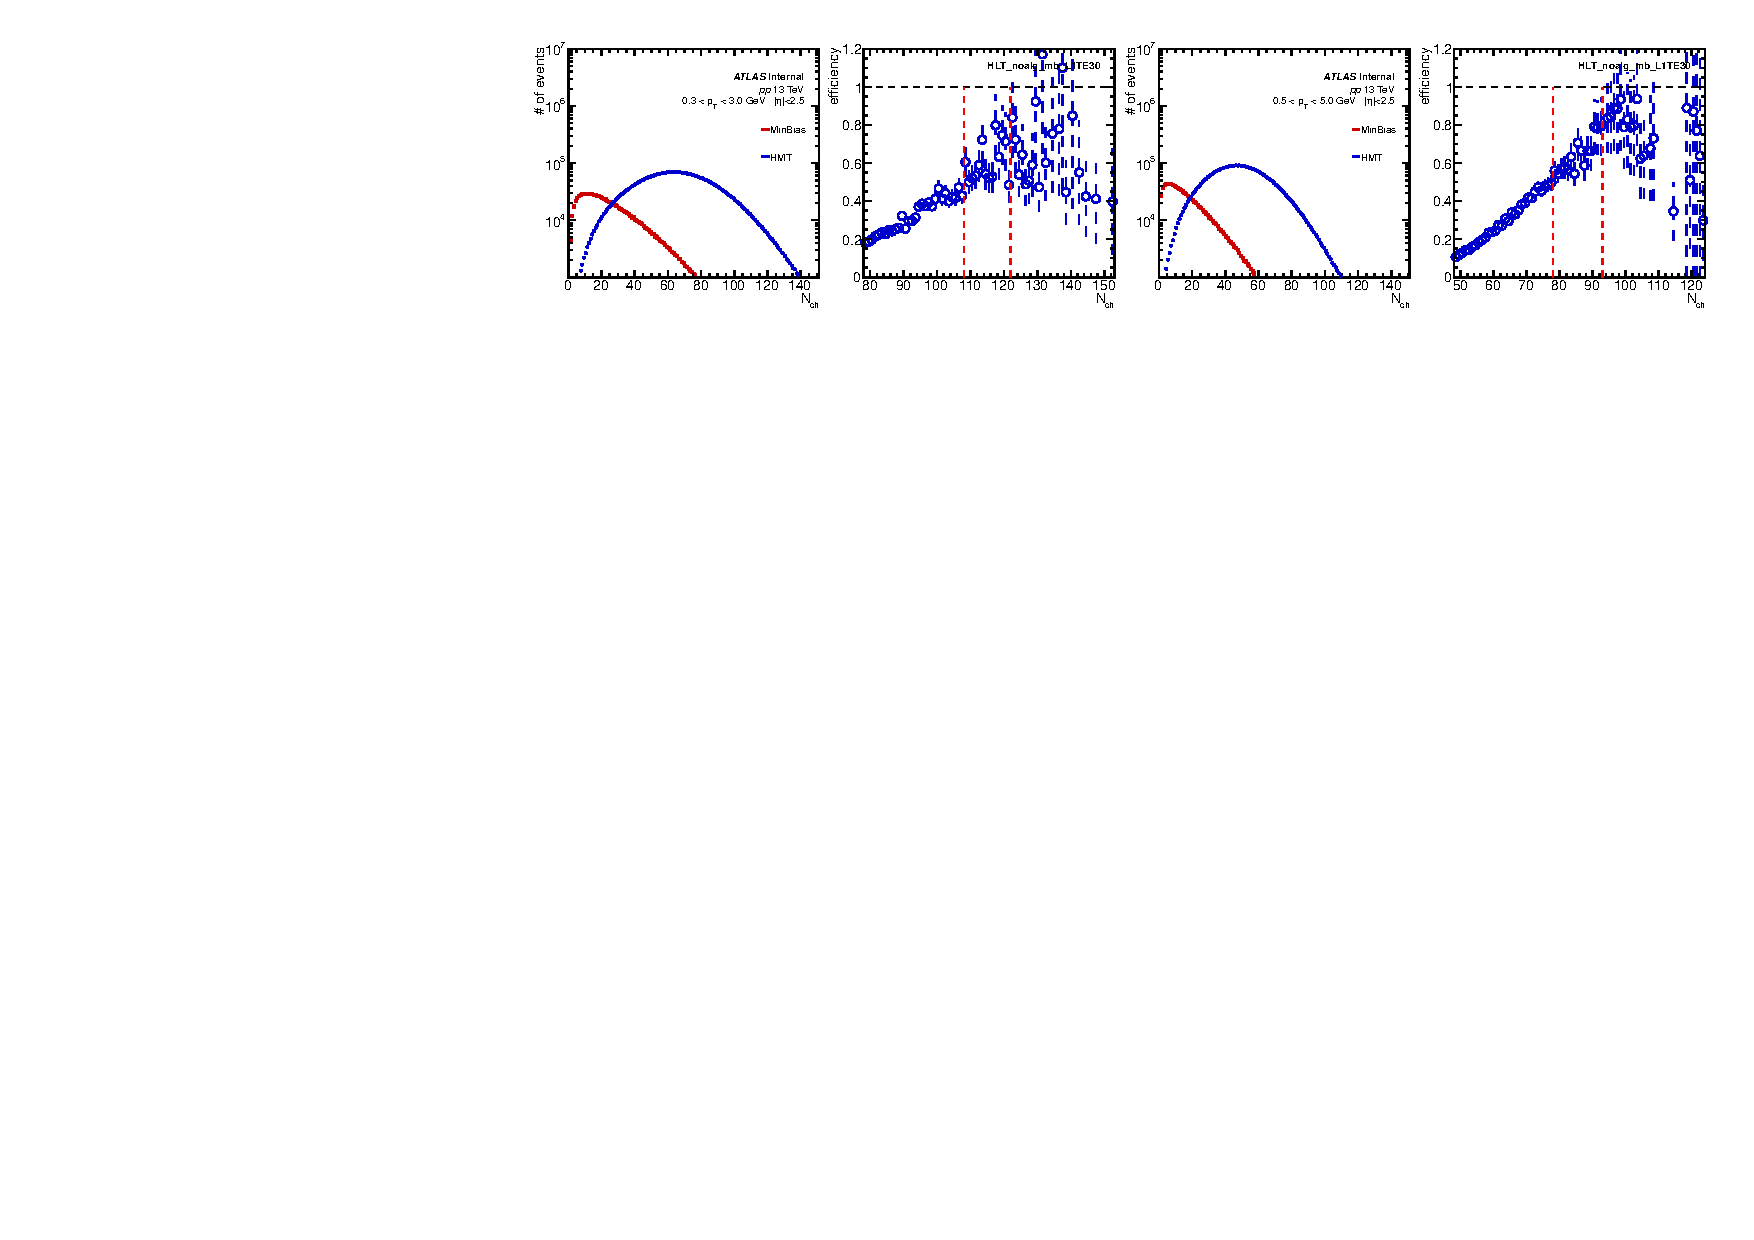
\includegraphics[width=1.\linewidth]{figs/sec_evtSlc/trigEff_pp13_run3/trigEff_Trig2.pdf}
\end{figure}
\begin{figure}[H]
\centering
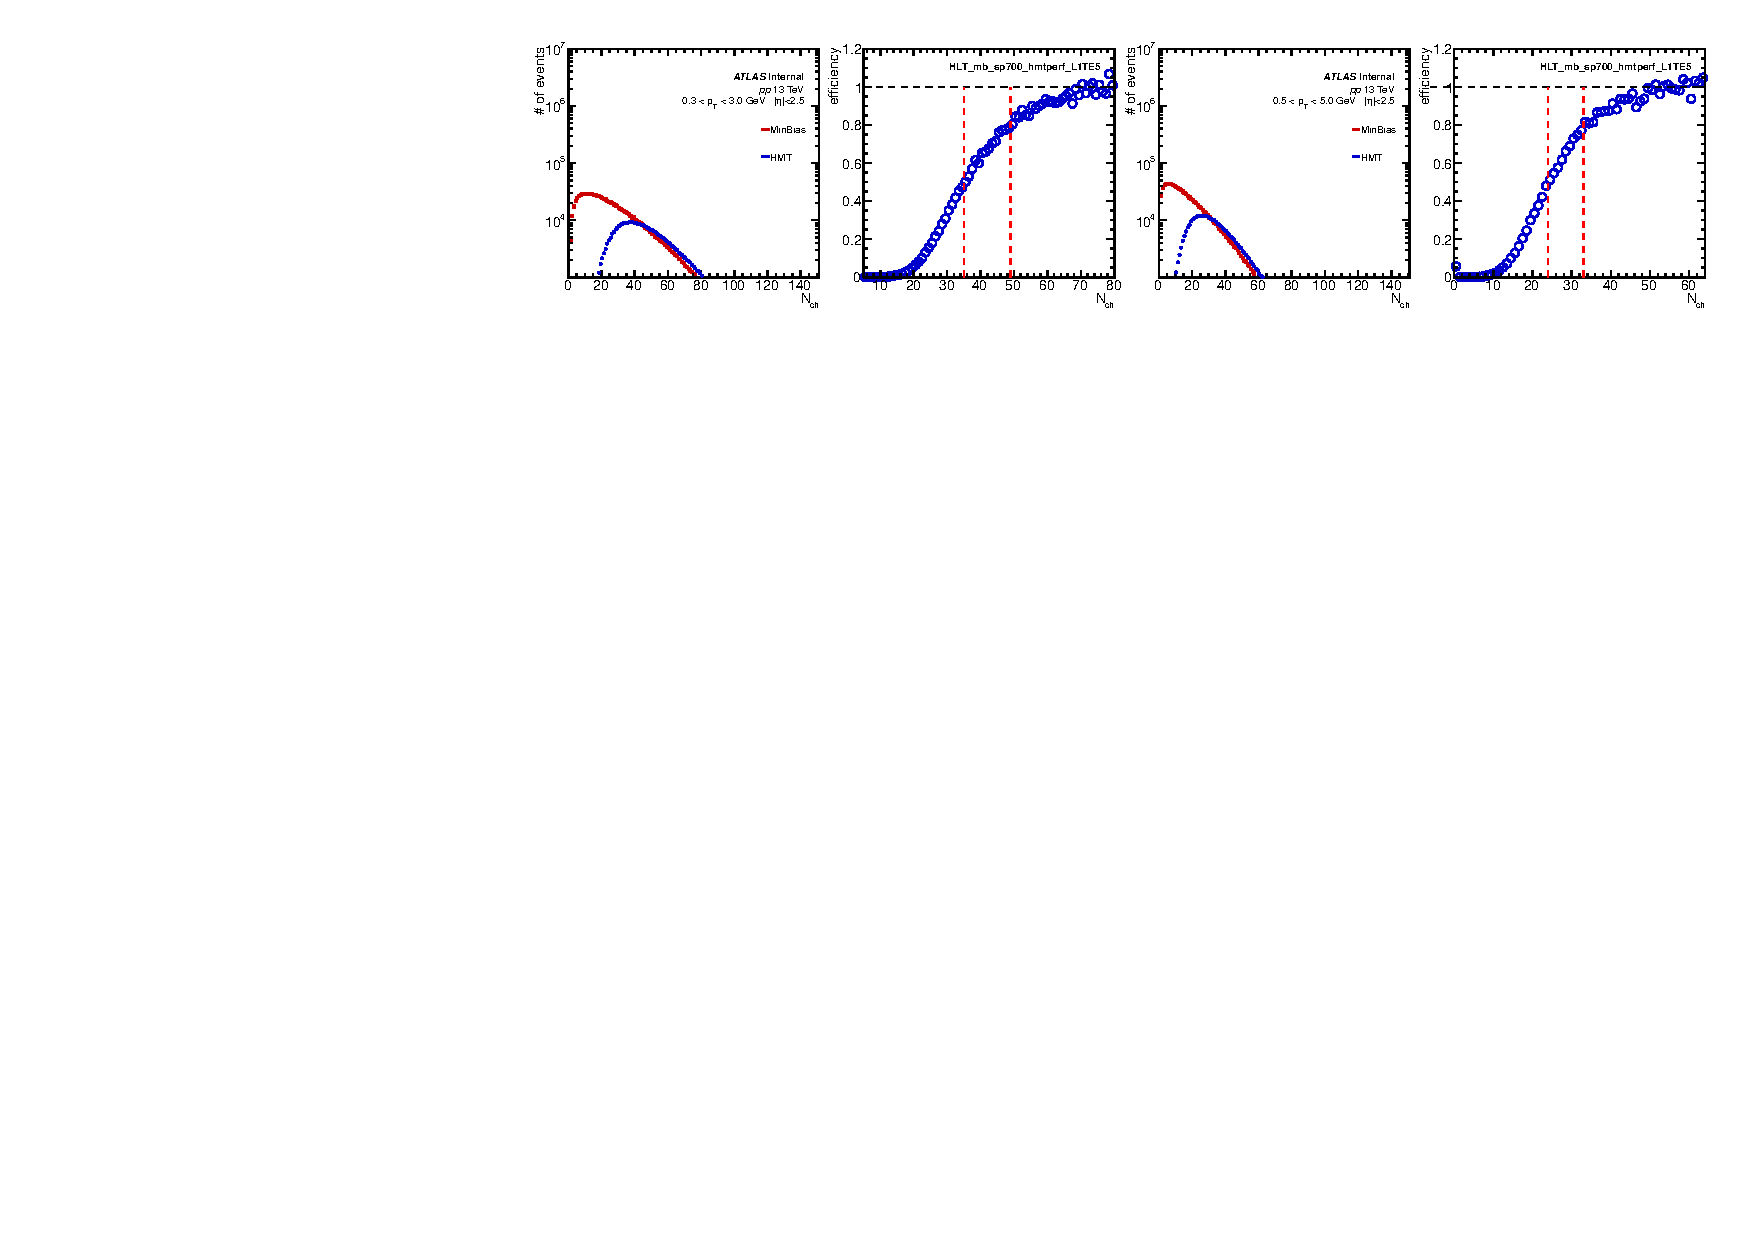
\includegraphics[width=1.\linewidth]{figs/sec_evtSlc/trigEff_pp13_run3/trigEff_Trig6.pdf}
\end{figure}
\begin{figure}[H]
\centering
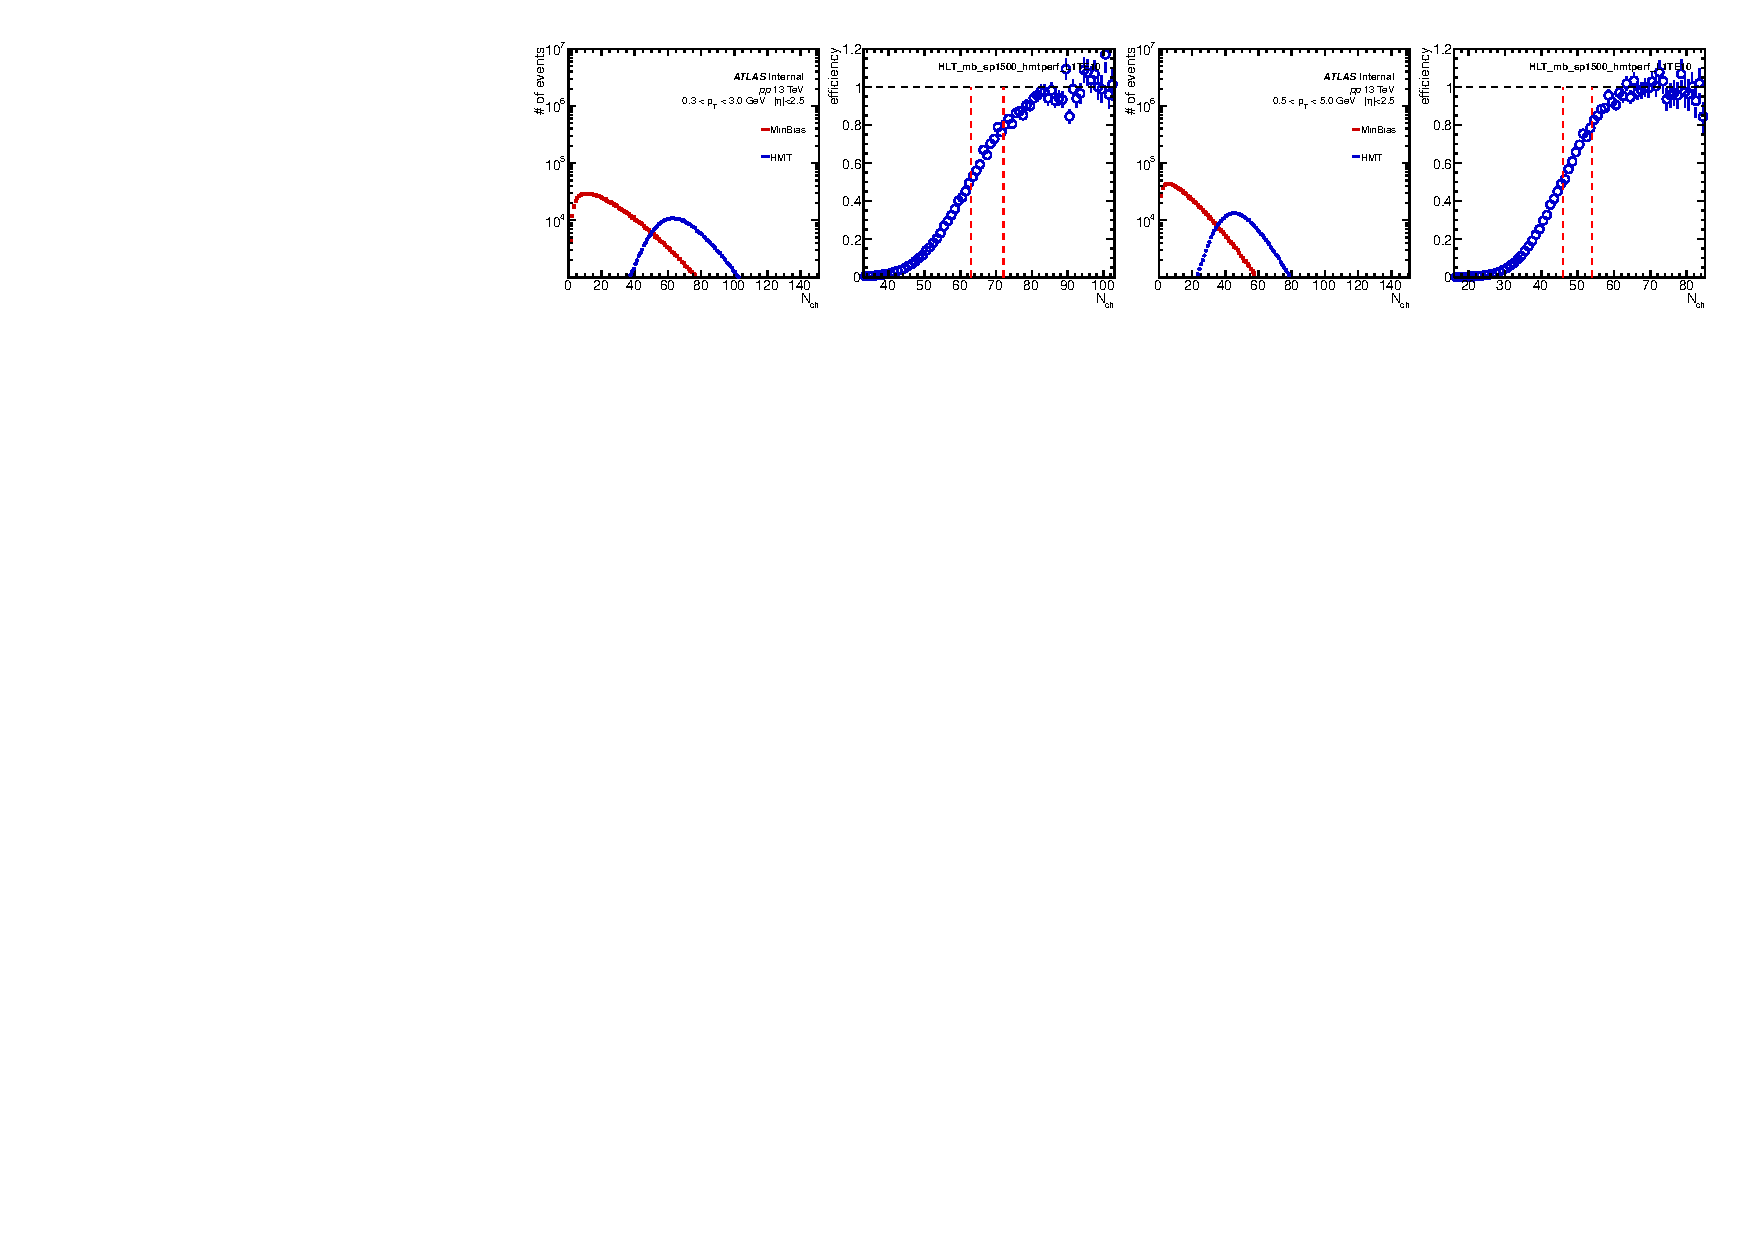
\includegraphics[width=1.\linewidth]{figs/sec_evtSlc/trigEff_pp13_run3/trigEff_Trig7.pdf}
\end{figure}
\begin{figure}[H]
\centering
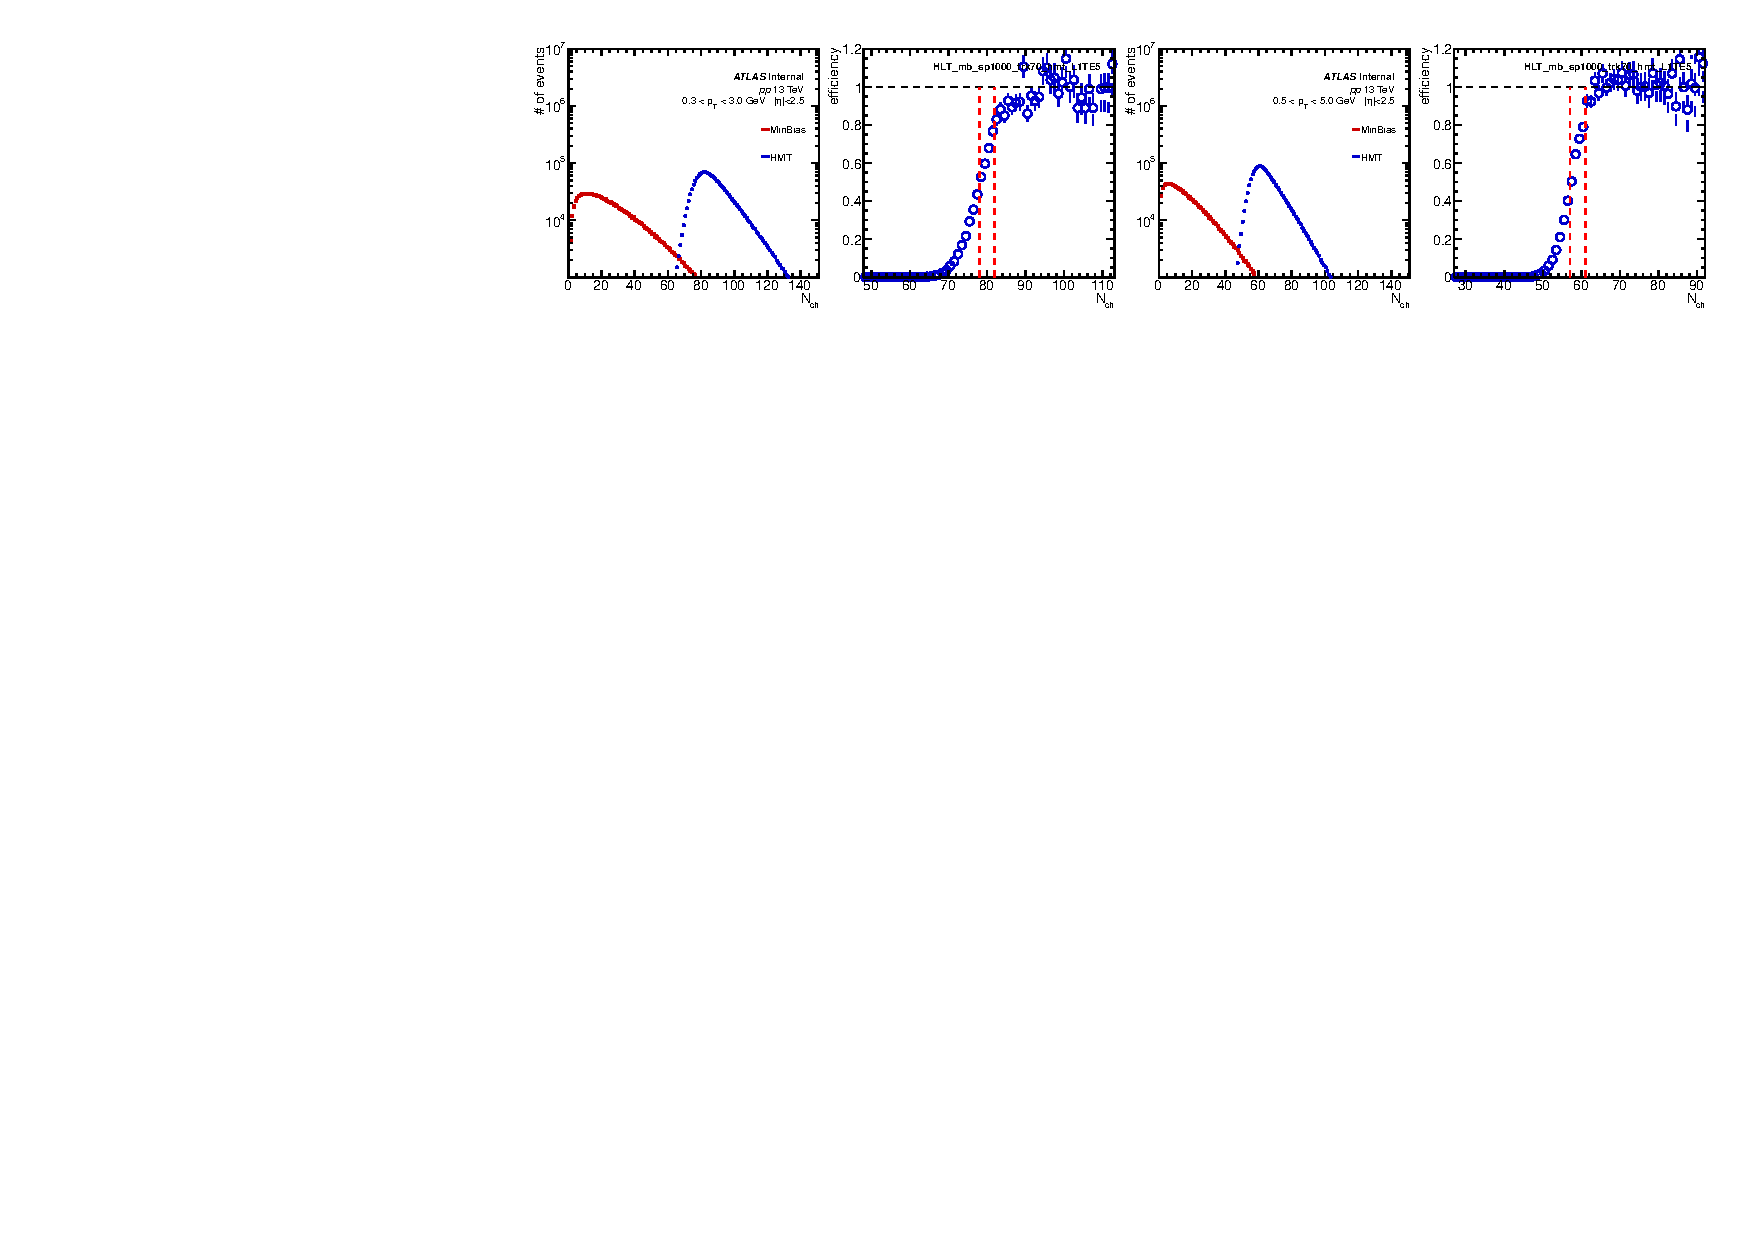
\includegraphics[width=1.\linewidth]{figs/sec_evtSlc/trigEff_pp13_run3/trigEff_Trig9.pdf}
\end{figure}
\begin{figure}[H]
\centering
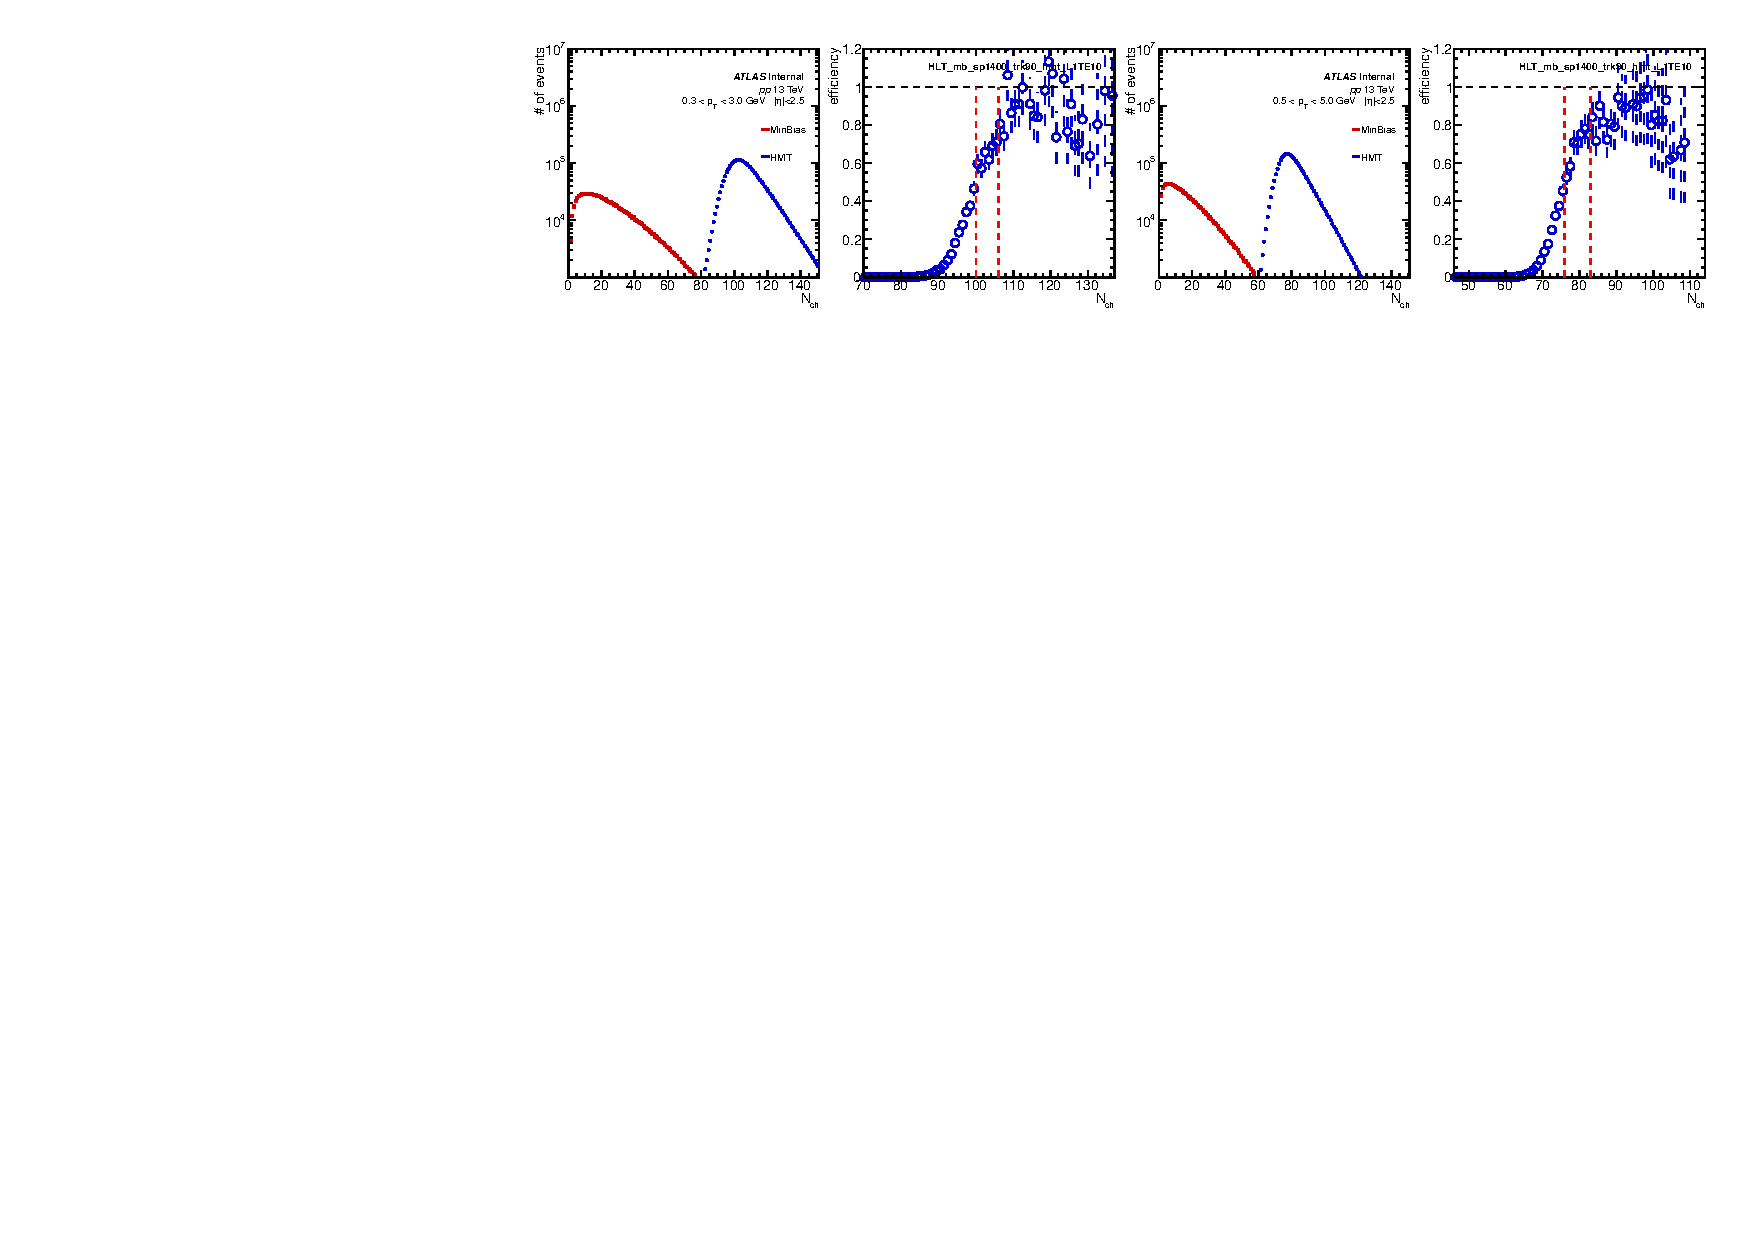
\includegraphics[width=1.\linewidth]{figs/sec_evtSlc/trigEff_pp13_run3/trigEff_Trig11.pdf}
\caption{Trigger efficiencies of all major HMT triggers as a function of number of tracks in two $p_{T}$ ranges: $0.3<p_{T}<3.0$ GeV and $0.5<p_{T}<5.0$ GeV, from 13 TeV $pp$ run period 3. Efficiency is calculated relative to the corresponding MinBias trigger in this run period then scaled to 1.0 in the large $N_{ch}$ region. The two red dash lines indicate 50$\%$ and 80$\%$ efficiency cuts.}
\label{fig:trigEff_pp13_run3}
\end{figure}
Trigger efficiencies of all the major HMT triggers are summarized in Fig.~\ref{fig:trigEff_pp13_run3}, where efficiencies are shown for two $p_{T}$ ranges separately: $0.3<p_{T}<3.0$ GeV and $0.5<p_{T}<5.0$ GeV.



\subsubsection{Run period 4}
The 4th run period data was taken in 2016 and there are 3 intermediate-$\mu$ runs used for this analysis:
\begin{itemize}

\item Run 309314, peak $\mu=0.36$, 13.2 million events
\begin{itemize}[leftmargin=*]
\item[] \verb|data16_13TeV.00309314.physics_MinBias.recon.AOD.r8576/|
\end{itemize}

\item Run 309346, peak $\mu=0.33$, 7.5 million events
\begin{itemize}[leftmargin=*]
\item[] \verb|data16_13TeV.00309346.physics_MinBias.recon.AOD.r8576/|
\end{itemize}

\item Run 310216, peak $\mu=0.31$, 79.9 million events
\begin{itemize}[leftmargin=*]
\item[] \verb|data16_13TeV.00310216.physics_MinBias.recon.AOD.r8600/|
\end{itemize}

\end{itemize}
The major MinBias and HMT triggers applied in this run period are:
\begin{itemize}
\item \verb|HLT_mb_sptrk|
\item \verb|HLT_mb_sp900_trk50_hmt_L1TE5|
\item \verb|HLT_mb_sp1000_trk70_hmt_L1TE10.0ETA24|
\item \verb|HLT_mb_sp1400_trk90_hmt_L1TE20.0ETA24|
\end{itemize}
where a new trigger item has been introduced:
\begin{itemize}
\item \verb|L1TEX.0ETA24|: L1 trigger is seeded at L1 total energy from the restricted $\eta$ range: $-2.4<\eta<2.4$ and the threshold is X GeV;
\end{itemize}

\begin{figure}[H]
\centering
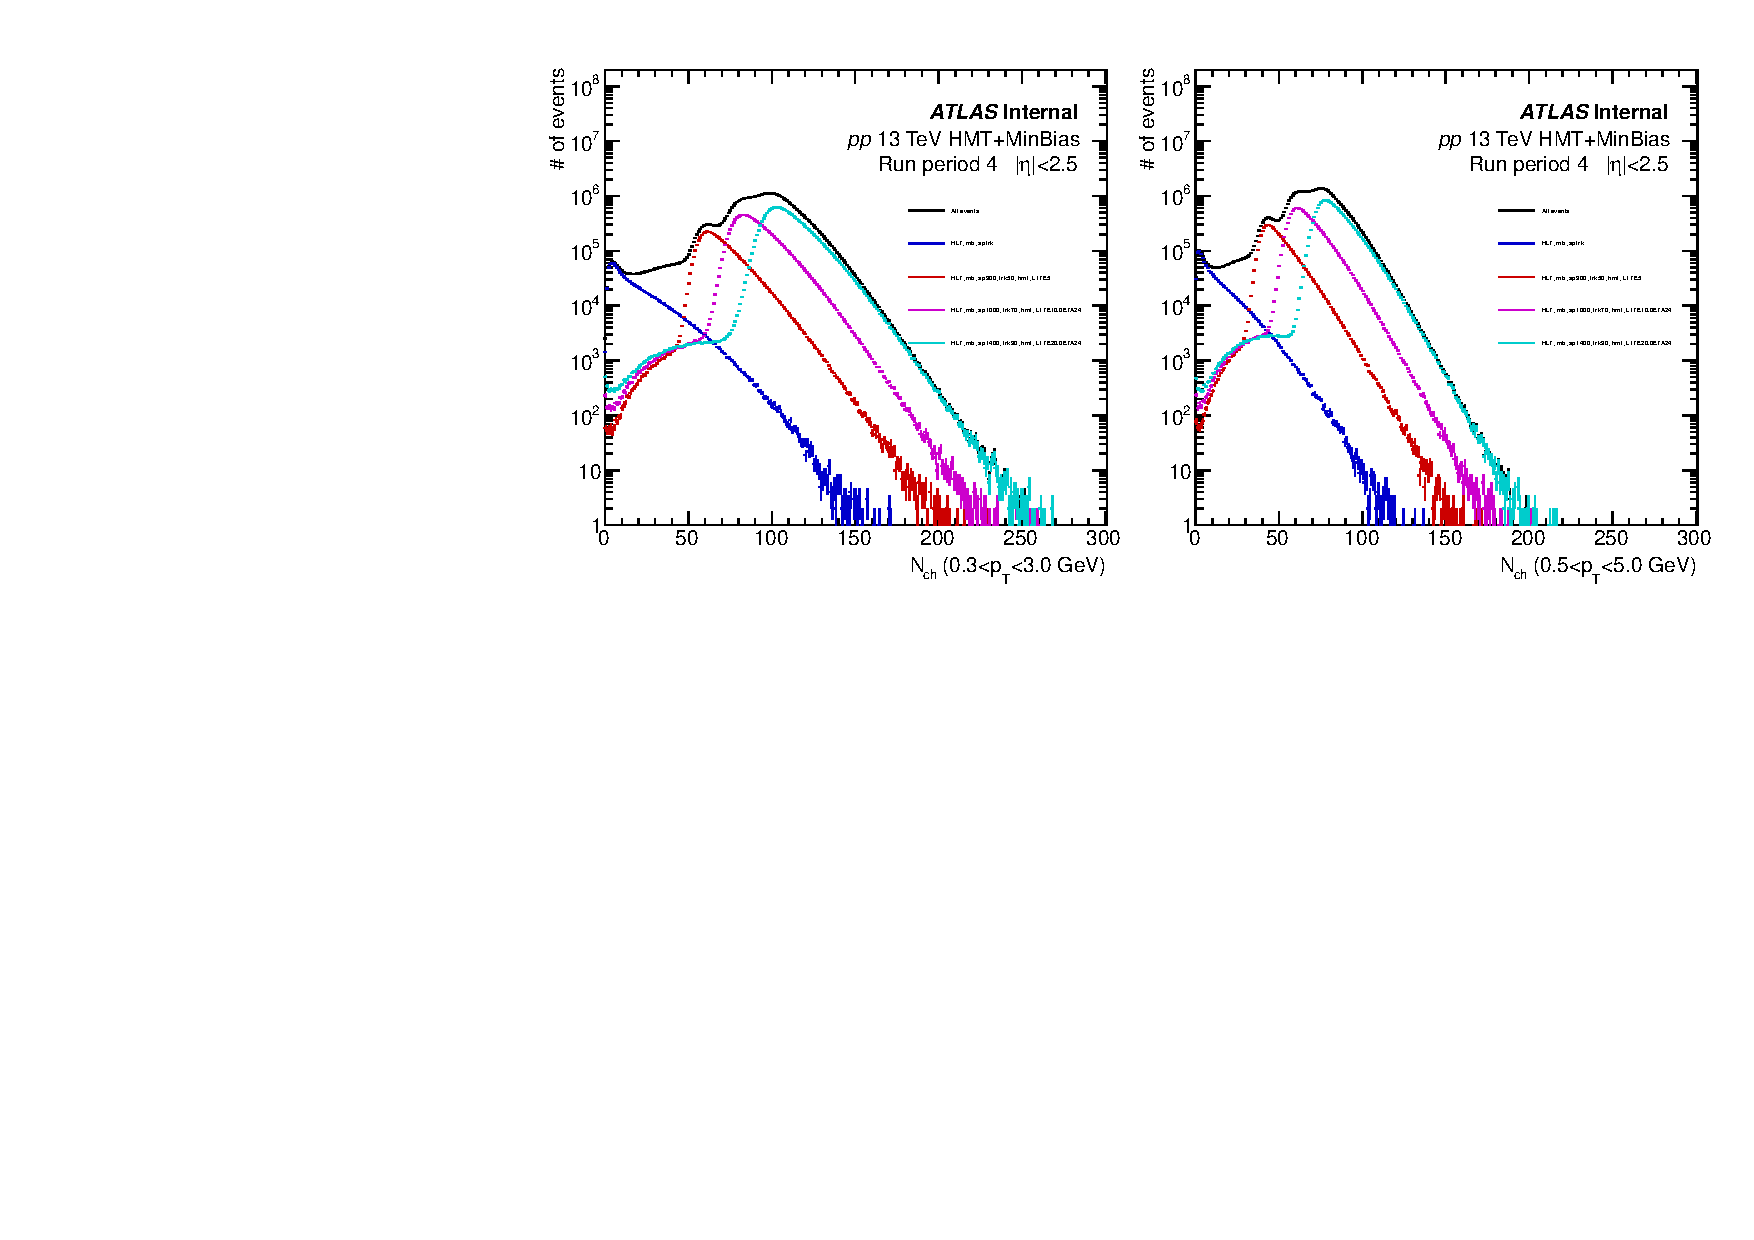
\includegraphics[width=.9\linewidth]{figs/sec_evtSlc/trkDis_pp13_run4.pdf}
\caption{Distribution of number of tracks with two $p_{T}$ thresholds: $0.3<p_{T}<3.0$ GeV and $0.5<p_{T}<5.0$ GeV, in 13 TeV $pp$ run period 4. The major MinBias and HMT triggers are plotted separately.}
\label{fig:trkDis_pp13_run4}
\end{figure}
The summary of statistics with all the major triggers used in this analysis are shown in Fig.~\ref{fig:trkDis_pp13_run4}.

\begin{figure}[H]
\centering
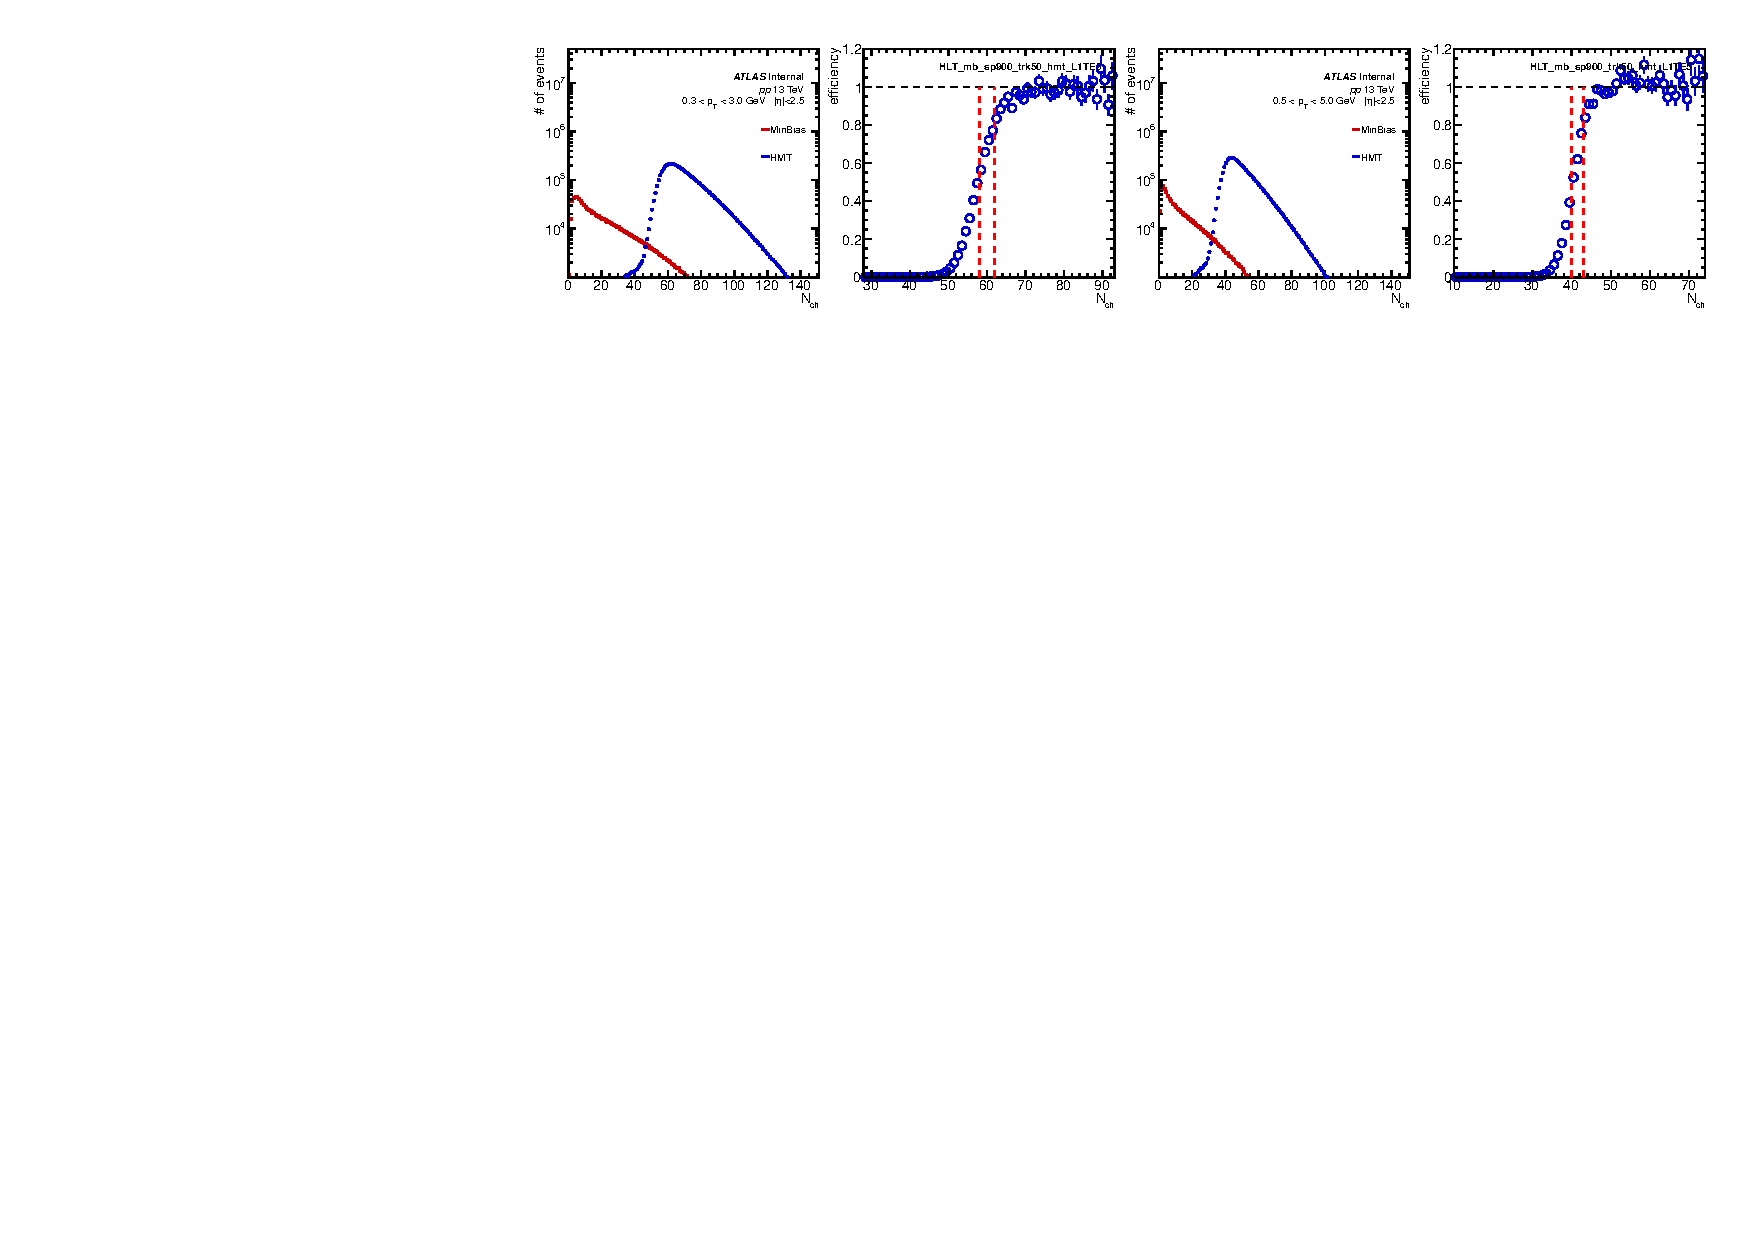
\includegraphics[width=1.\linewidth]{figs/sec_evtSlc/trigEff_pp13_run4/trigEff_Trig18.pdf}
\end{figure}
\begin{figure}[H]
\centering
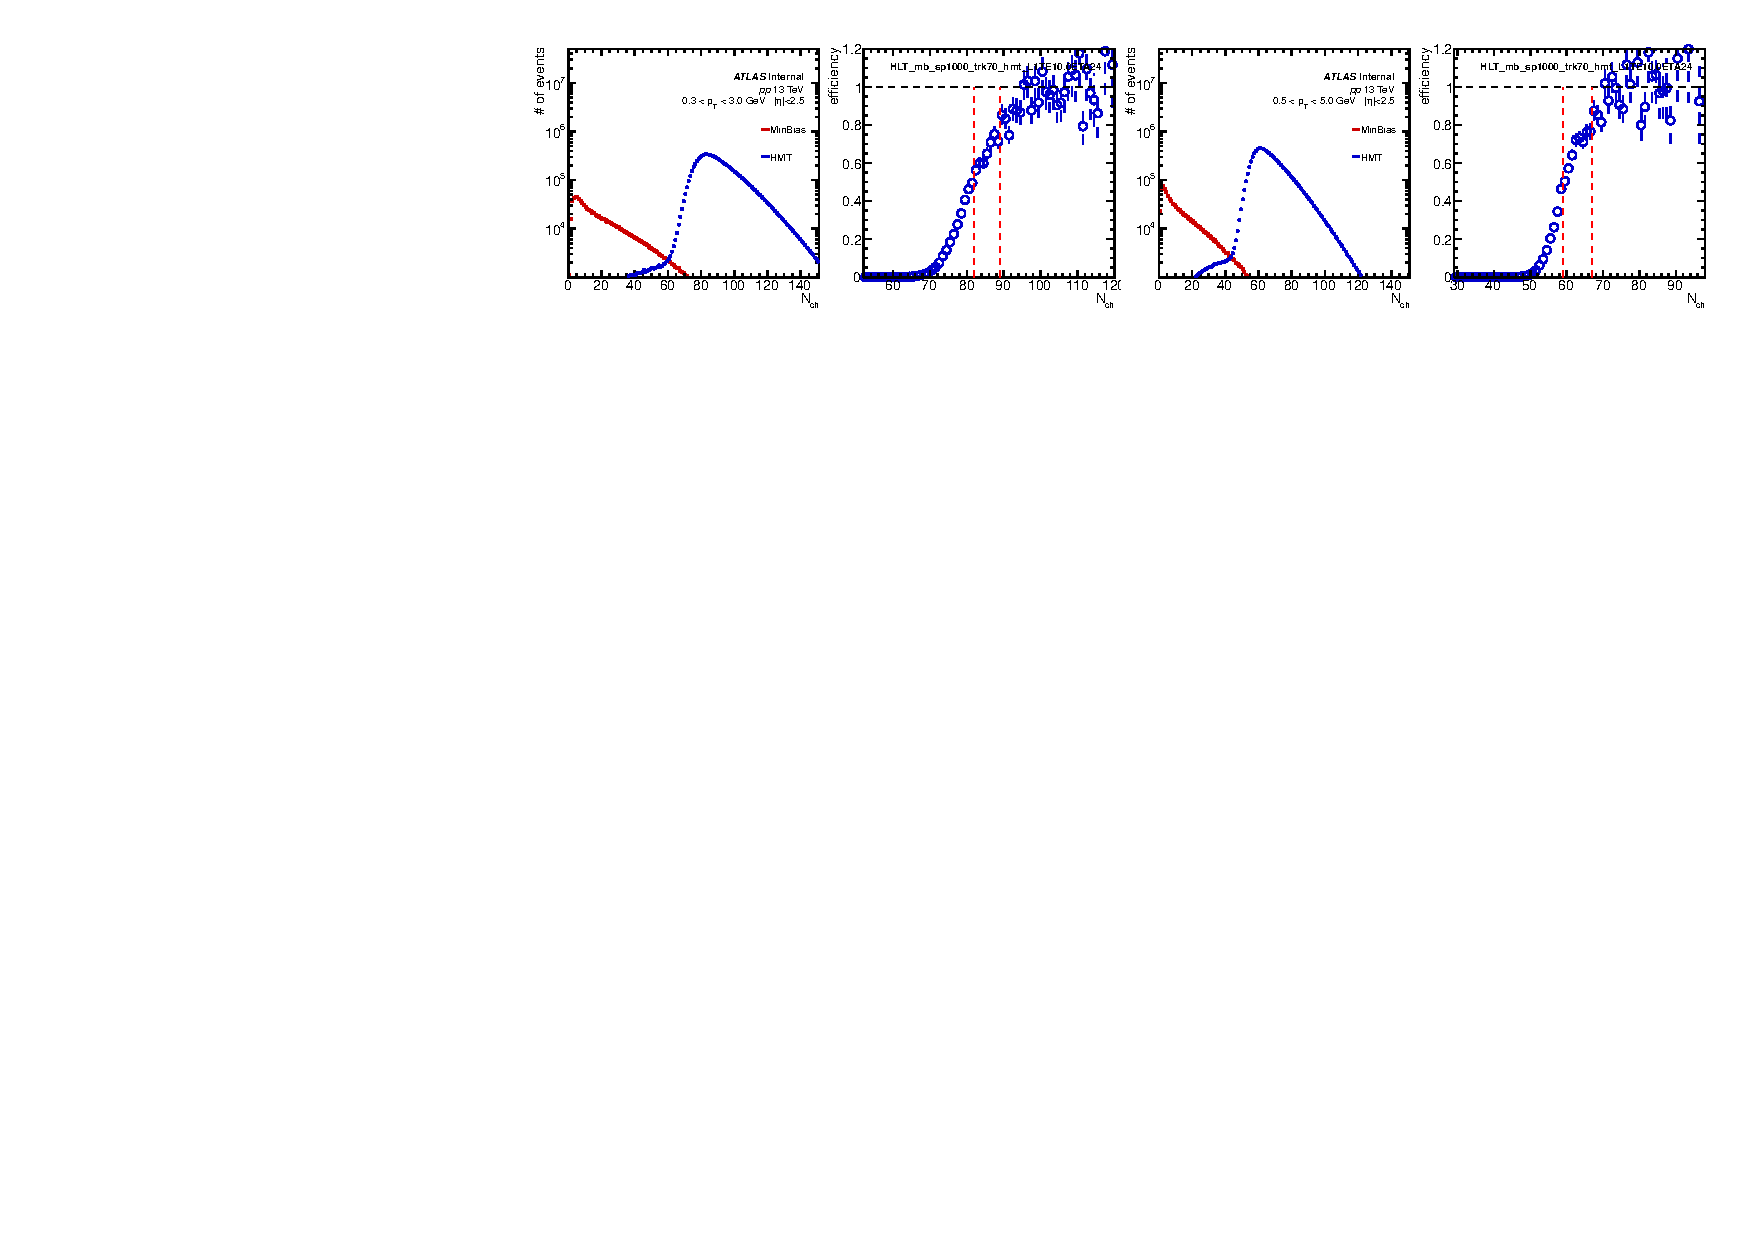
\includegraphics[width=1.\linewidth]{figs/sec_evtSlc/trigEff_pp13_run4/trigEff_Trig24.pdf}
\end{figure}
\begin{figure}[H]
\centering
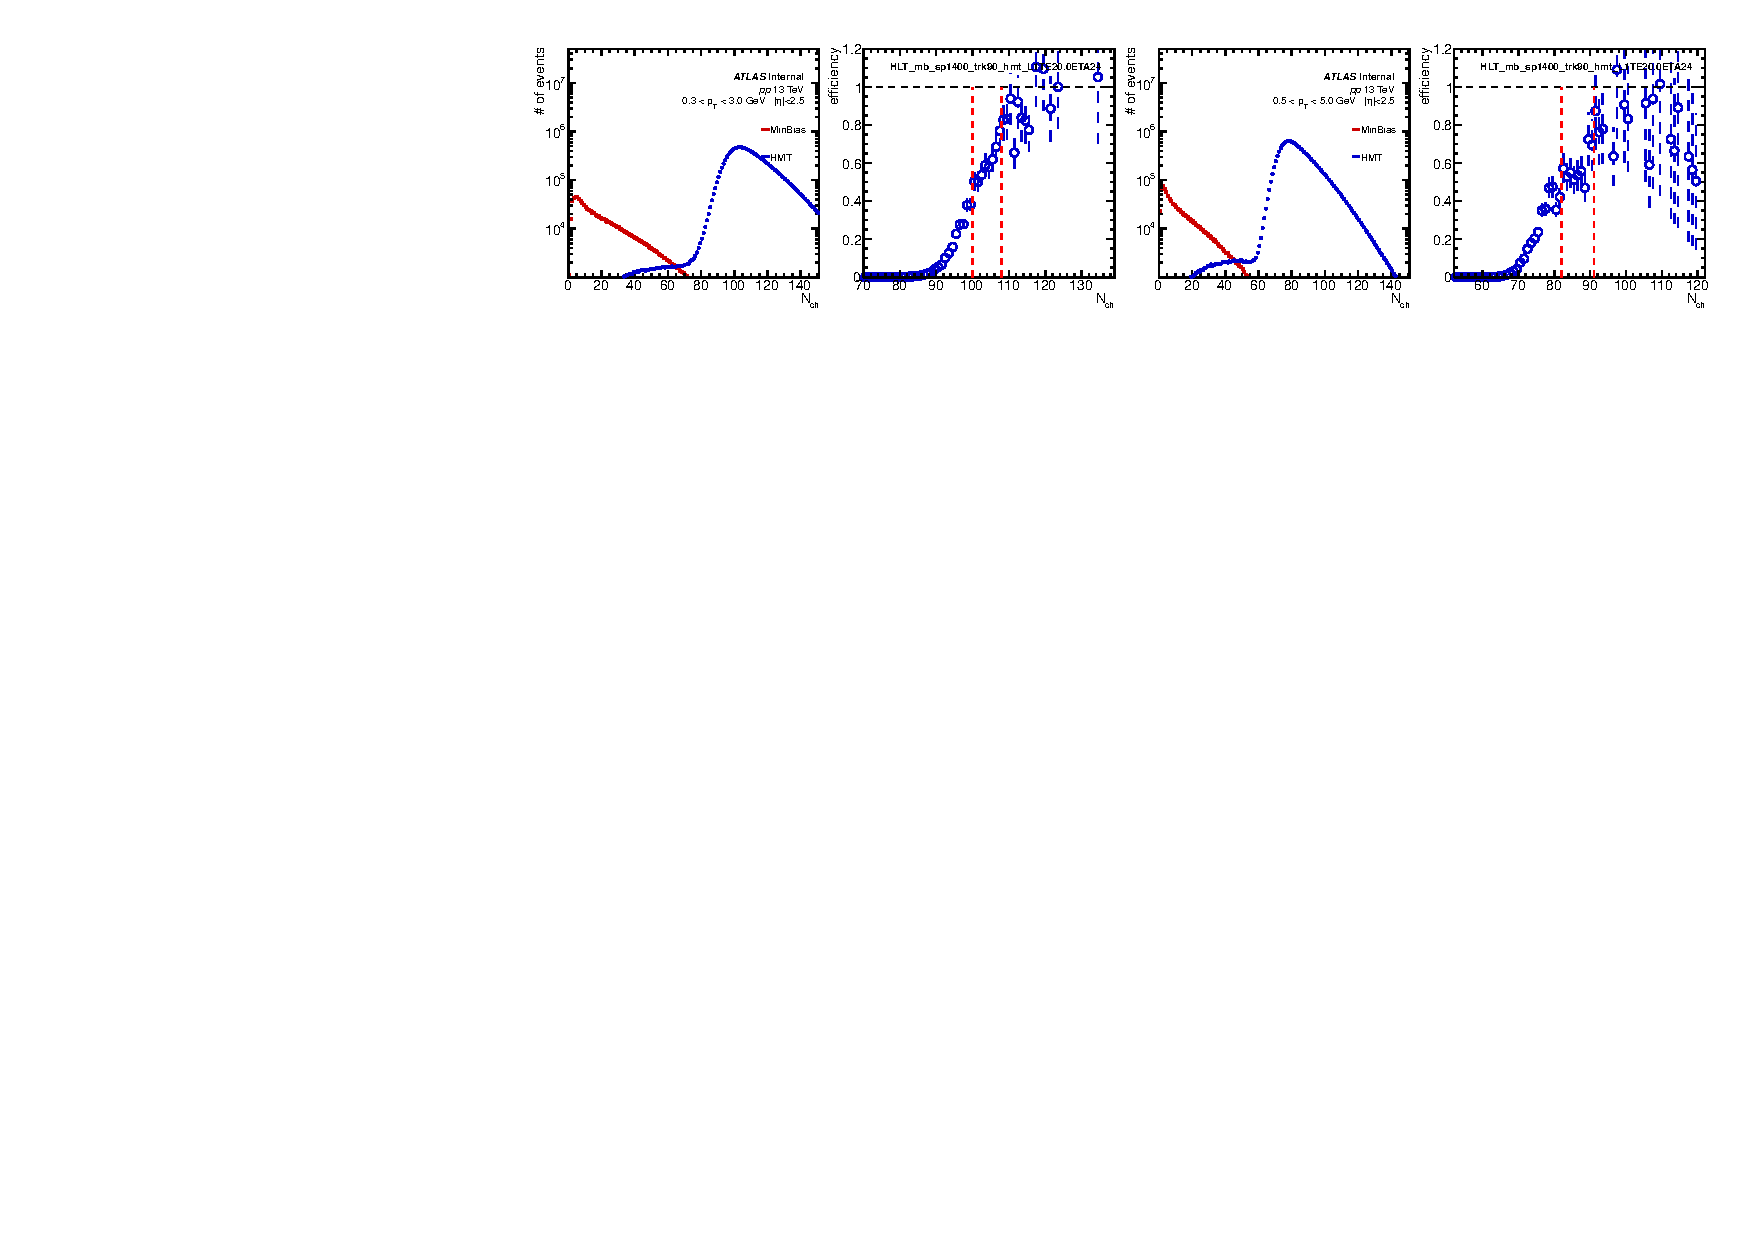
\includegraphics[width=1.\linewidth]{figs/sec_evtSlc/trigEff_pp13_run4/trigEff_Trig30.pdf}
\caption{Trigger efficiencies of all major HMT triggers as a function of number of tracks in two $p_{T}$ ranges: $0.3<p_{T}<3.0$ GeV and $0.5<p_{T}<5.0$ GeV, from 13 TeV $pp$ run period 4. Efficiency is calculated relative to the corresponding MinBias trigger in this run period then scaled to 1.0 in the large $N_{ch}$ region. The two red dash lines indicate 50$\%$ and 80$\%$ efficiency cuts.}
\label{fig:trigEff_pp13_run4}
\end{figure}
Trigger efficiencies of all the major HMT triggers are summarized in Fig.~\ref{fig:trigEff_pp13_run4}, where efficiencies are shown for two $p_{T}$ ranges separately: $0.3<p_{T}<3.0$ GeV and $0.5<p_{T}<5.0$ GeV.



\subsubsection{PYTHIA for $pp$ 13 TeV data}

The tracking efficiency applied in this analysis were identical to the ATLAS previous cumulant measurement \verb|ATL-COM-PHYS-2015-740|. The following studies are independent to the other analysis team, and the final results of $c_{2}{4}$ are checked to be consistent no matter which tracking efficiency map is applied.

The PYTHIA~\cite{Sjostrand:2007gs} A2 tune~\cite{atlas:6} was used to produce $pp$ collisions with the same energy as in the data. The detector response is simulated with GEANT 4 with conditions matching those present during the data-taking. The simulated events are reconstructed with the same algorithms as data, in particular using the same track reconstruction as for the data.

The list of PYTHIA samples is shown in the following:
\begin{itemize}
\item 20 million ND sample
\begin{itemize}[leftmargin=*]
\item[] \verb|mc15_13TeV.361203.Pythia8_A2_MSTW2008LO_ND_minbias.merge.AOD.|
\item[] \verb|e3639_a782_a787_r6264/|
\end{itemize}
\item 1 million HMT sample with $N_{ch}>120$
\begin{itemize}[leftmargin=*]
\item[] \verb|mc15_13TeV.361214.Pythia8_A2MSTW2008LO_minbias_NDnch120.merge.AOD.|
\item[] \verb|e3908_a782_a787_r6264/|
\end{itemize}
\item 1 million HMT sample with $N_{ch}>160$
\begin{itemize}[leftmargin=*]
\item[] \verb|mc15_13TeV.361215.Pythia8_A2MSTW2008LO_minbias_NDnch160.merge.AOD.|
\item[] \verb|e3908_a782_a787_r6264/|
\end{itemize}
\item 1 million HMT sample with $N_{ch}>200$
\begin{itemize}[leftmargin=*]
\item[] \verb|mc15_13TeV.361216.Pythia8_A2MSTW2008LO_minbias_NDnch200.merge.AOD.|
\item[] \verb|e3908_a782_a787_r6264/|
\end{itemize}
\end{itemize}



To study the tracking performance, the same track selection requirements were applied to PYTHIA as 13 TeV data.

For the reconstructed tracks, the primary tracks are defined as:
\begin{itemize}
\item Pass the track selection requirements
\item Truth match $\text{probability}>0.5$
\item Associated truth particle is a primary particle
\end{itemize}
where primary particle is defined on the truth level:
\begin{itemize}
\item $\text{Status}=1$, $\text{charge}!=0$
\item $p_{T}>200$ MeV
\item $|\eta|\le 2.5$
\item $0<\text{Barcode}<2e5$
\item strange baryons are excluded
\end{itemize}

The tracking efficiency $\epsilon$ is then defined as:
\begin{equation}
\epsilon(p_{T},\eta,N_{ch},z_{vtx})\equiv\frac{N_{ch}^{primary}}{N_{ch}^{truth}}
\end{equation}
where $N_{ch}^{primary}$ denotes the number of primary tracks on reconstructed level and $N_{ch}^{truth}$ denotes the number of primary particles on truth level. In previous $pp$ analysis, the tracking efficiency is measure only as a function of $p_{T}$ and $\eta$. To evaluate the possible variation due to changing $N_{ch}$ (In this analysis, $N_{ch}$ is defined as number of reconstructed tracks with $p_{T}>0.4$ GeV.) and $z_{vtx}$, we also added these two into the efficiency map.

The fake track is defined as:
\begin{itemize}
\item Pass the track selection requirements
\item Fulfill one of the following:
\begin{itemize}
\item Truth match $\text{probability}<0.5$
\item Not associated with truth particle
\item $\text{Barcode}=0$ of associated truth particle
\end{itemize}
\end{itemize}

Then the fraction of fake tracks $f$ is defined as:
\begin{equation}
f(p_{T},\eta,N_{ch}^{primary},z_{vtx})\equiv\frac{N_{ch}^{fake}}{N_{ch}^{primary}+N_{ch}^{fake}}
\end{equation}
where $N_{ch}^{fake}$ denotes the number of fake tracks.

To compensate the contribution from fake tracks, the efficiency $\epsilon$ can be corrected by defining $\epsilon'$
\begin{equation}
\epsilon'(p_{T},\eta,N_{ch},z_{vtx})\equiv\frac{N_{ch}^{primary}+N_{ch}^{fake}}{N_{ch}^{truth}}=\frac{\epsilon}{1-f}
\end{equation}
where in this definition an additional correction of $1-f$ is added to the tracking efficiency $\epsilon$.

As the $z$ position of the vertex changes, average multiplicity distribution along $\eta$ will also change slightly. To evaluable the impact due to the vertex position changes, the efficiency and fake fraction are determined as a function of $z_{vtx}$. Furthermore, the efficiency could also change slightly for different $N_{ch}$ region, so the efficiency and fake fraction are also measured as a function of $N_{ch}$.

\begin{figure}[H]
\centering
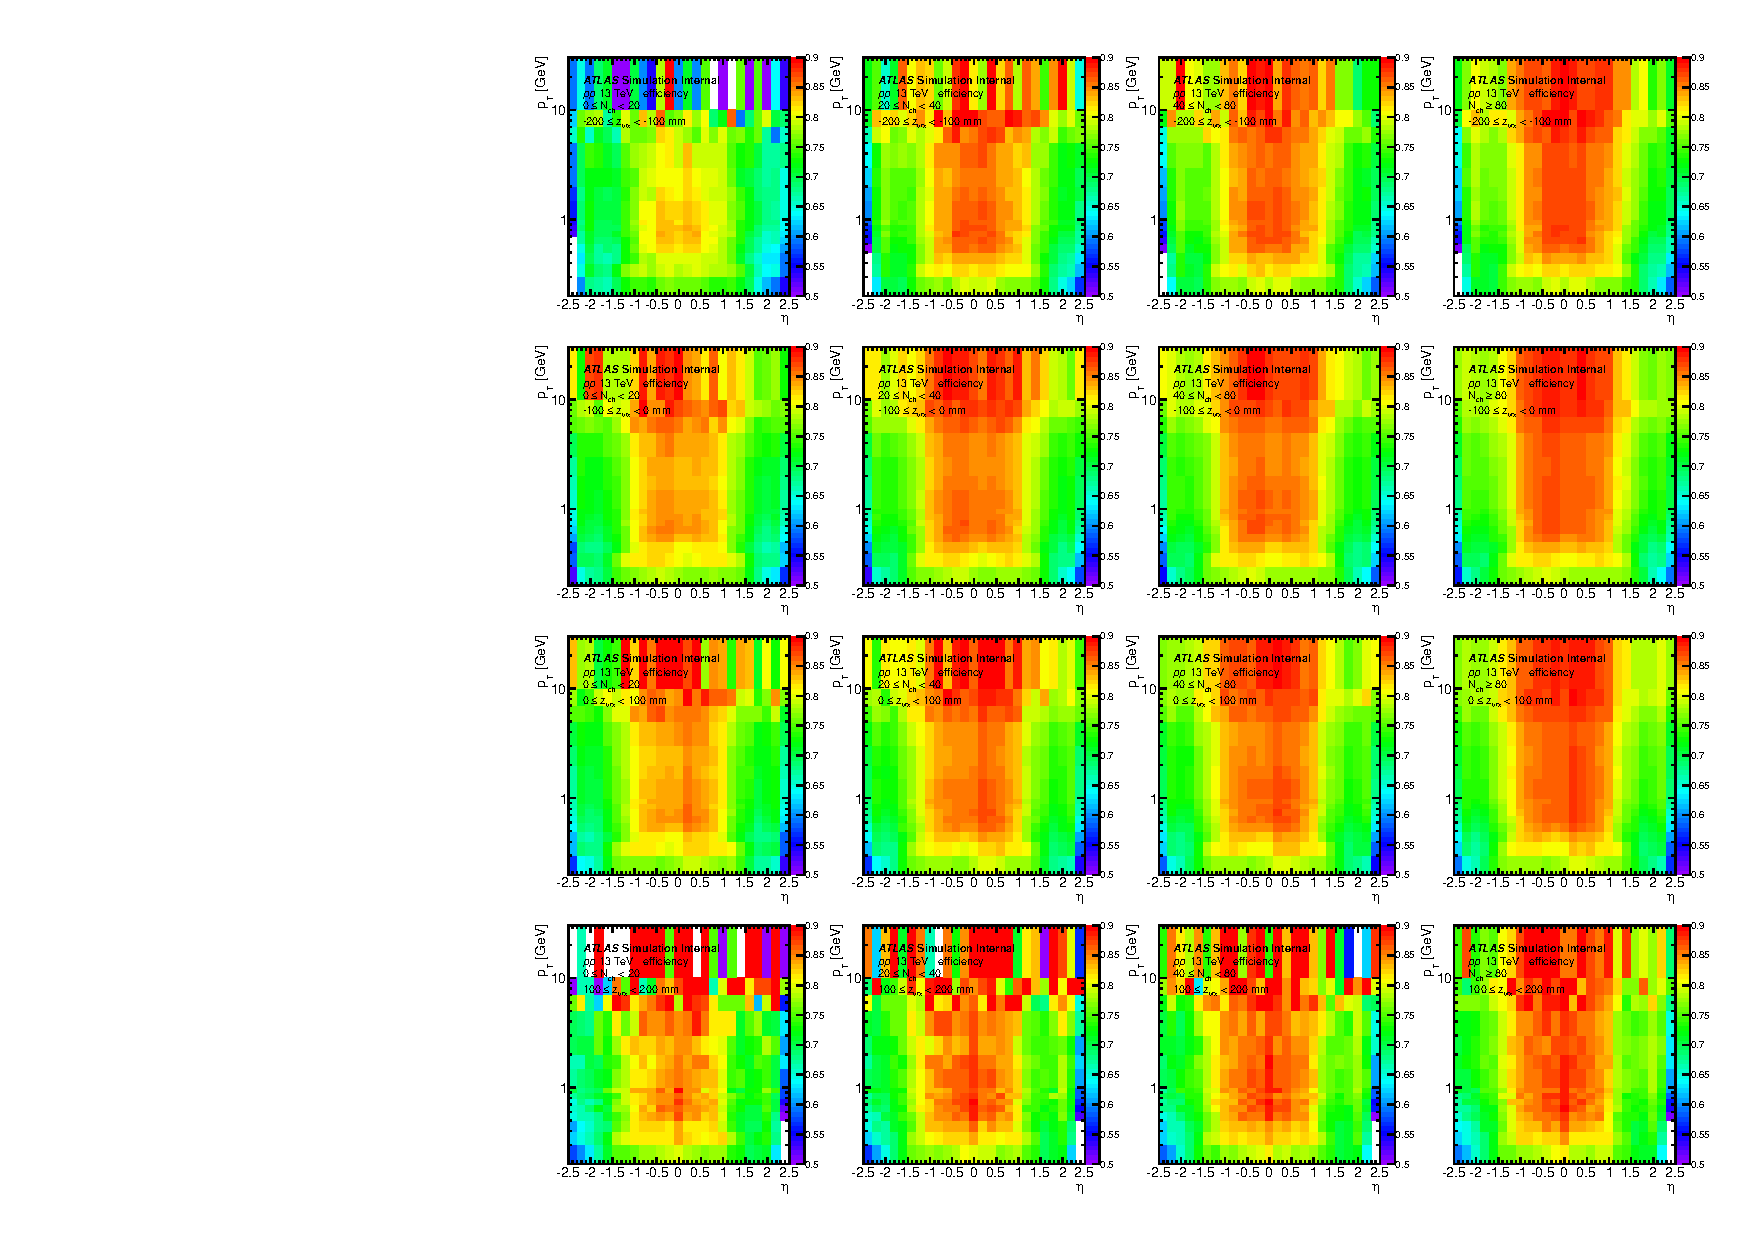
\includegraphics[width=1.\linewidth]{figs/sec_evtSlc/trkEff_pp13_eff_2D_wZvtx.pdf}
\caption{Tracking efficiency $\epsilon(\eta,p_{T})$. Each column is for different $N_{ch}$ ranges, and each row is for different $z_{vtx}$ range.}
\label{fig:trkEff_pp13_eff_2D_wZvtx}
\end{figure}

The efficiency $\epsilon(p_{T},\eta,N_{ch},z_{vtx})$ is summarized in Fig.~\ref{fig:trkEff_pp13_eff_2D_wZvtx}, where different rows represent different $z_{vtx}$ and different columns for different $N_{ch}$ ranges. The efficiency is not uniform in $\eta$: higher in mid$-\eta$ region. It is also not uniform along $p_{T}$: high$-p_{T}$ has higher efficiency. In this analysis, the default $p_{T}$ range is either $0.3<p_{T}<3.0$ GeV or $0.5<p_{T}<5.0$ GeV, and in the plots the $p_{T}$ starts from 0.2 GeV. So the efficiency is in low$-p_{T}$ is still above $60\%$. Moving from low$-N_{ch}$ to high$-N_{ch}$ the efficiency slightly increases: evaluating $\epsilon$ in different $N_{ch}$ is thus required. However, when move from $z_{vtx}~-200$ mm to $z_{vtx}~200$ mm, the efficiency doesn't change much. To gain better statistics, we decide to merge different $z_{vtx}$ ranges when applying efficiency in the data. Besides, since this measurement is not sensitive to rapidity, the minimal changes of the efficiency as a function of $z_{vtx}$ only have negligible impact on the final results.

\begin{figure}[H]
\centering
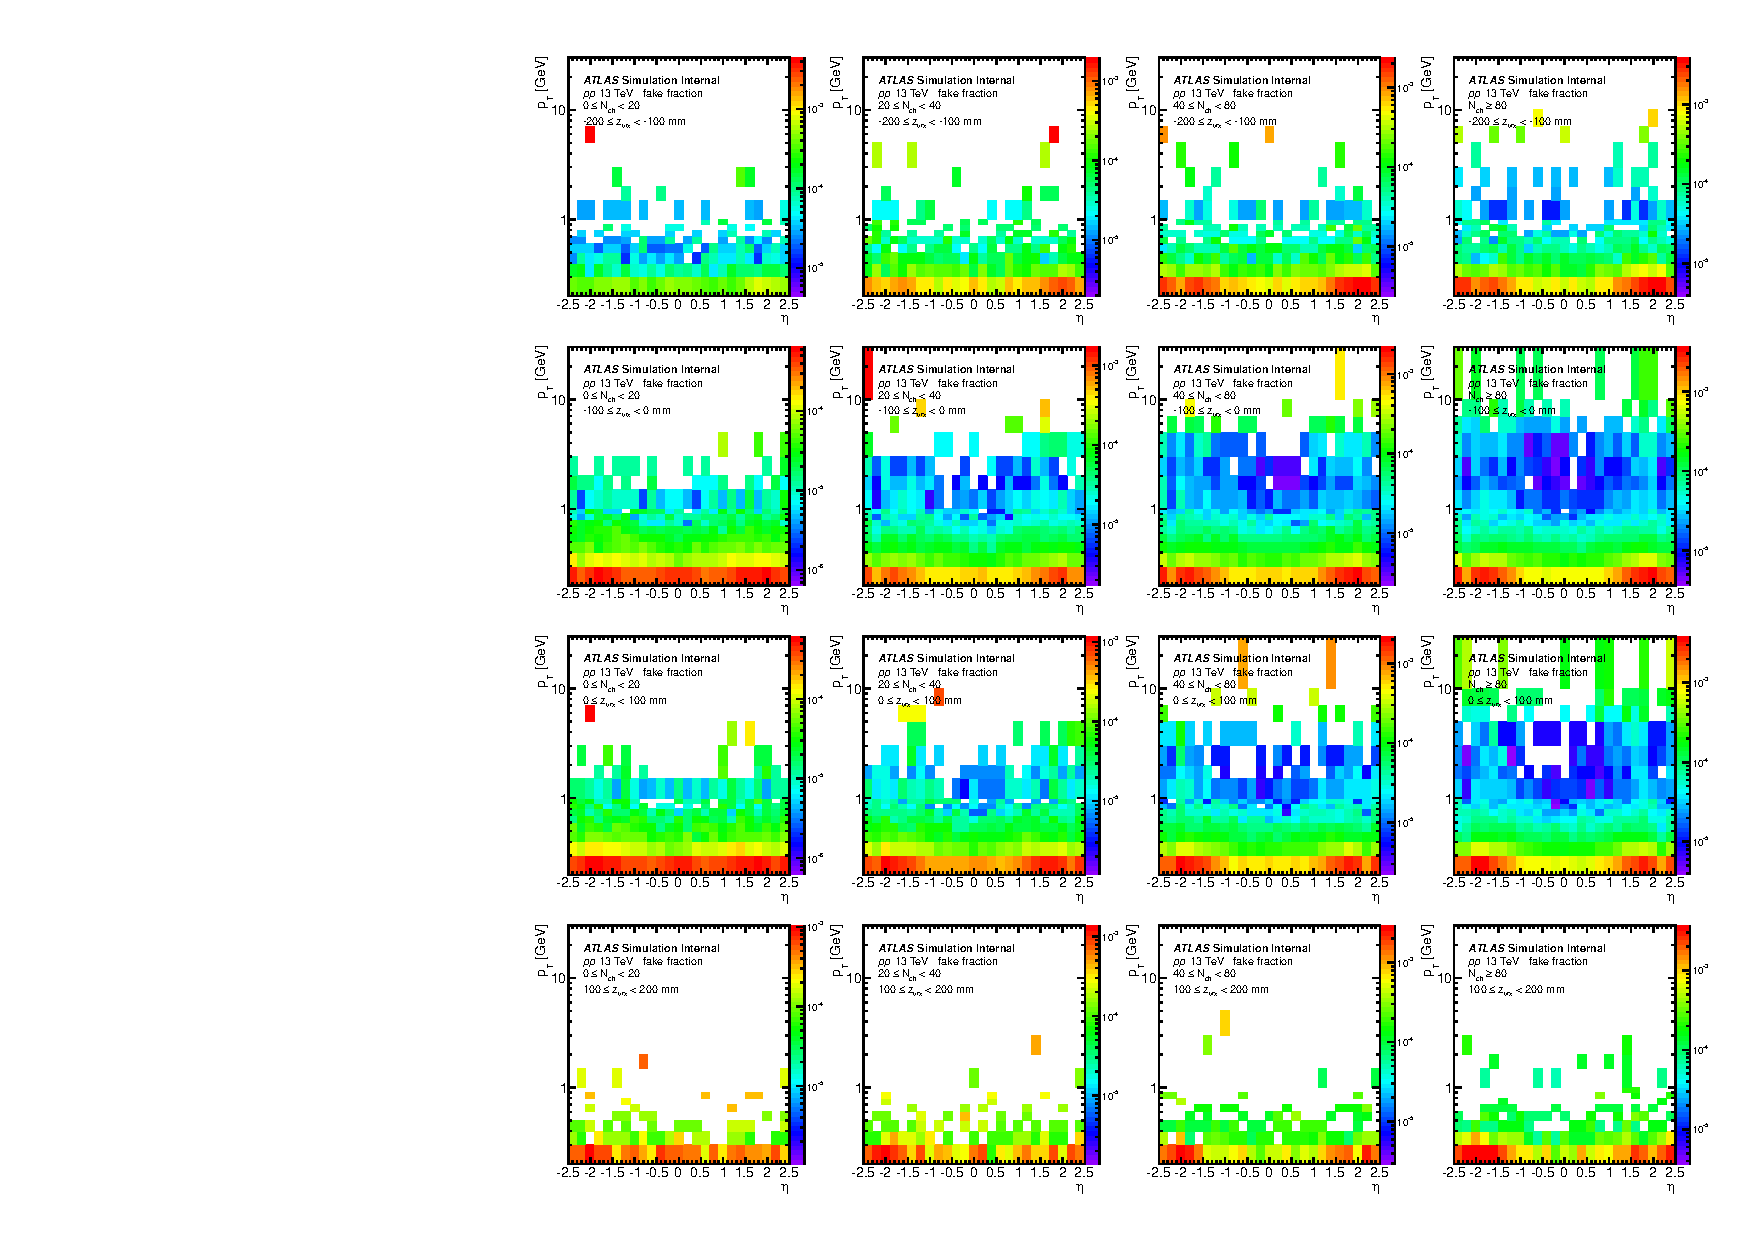
\includegraphics[width=1.\linewidth]{figs/sec_evtSlc/trkEff_pp13_fak_2D_wZvtx.pdf}
\caption{Fake fraction $f(\eta,p_{T})$. Each column is for different $N_{ch}$ ranges, and each row is for different $z_{vtx}$ range.}
\label{fig:trkEff_pp13_fak_2D_wZvtx}
\end{figure}

Fig.~\ref{fig:trkEff_pp13_fak_2D_wZvtx} summaries the fake fraction $f(\eta,p_{T})$ for different $z_{vtx}$ and $N_{ch}$ ranges, where the layouts of the panels are same as previous efficiency plots. The fake fraction is higher in the low$-p_{T}$ region and is consistent with 0 in high$-p_{T}$. The fake fraction is also $\eta$ dependent, but opposite to efficiency: lower in mid-$\eta$. Overall the fake fraction is on the level of below $0.1\%$. Like efficiency, the fake fraction is also dependent of $N_{ch}$, and has very weak dependence of $z_{vtx}$. So we will merge the fake fraction map among different $z_{vtx}$ ranges in the end.

\begin{figure}[H]
\centering
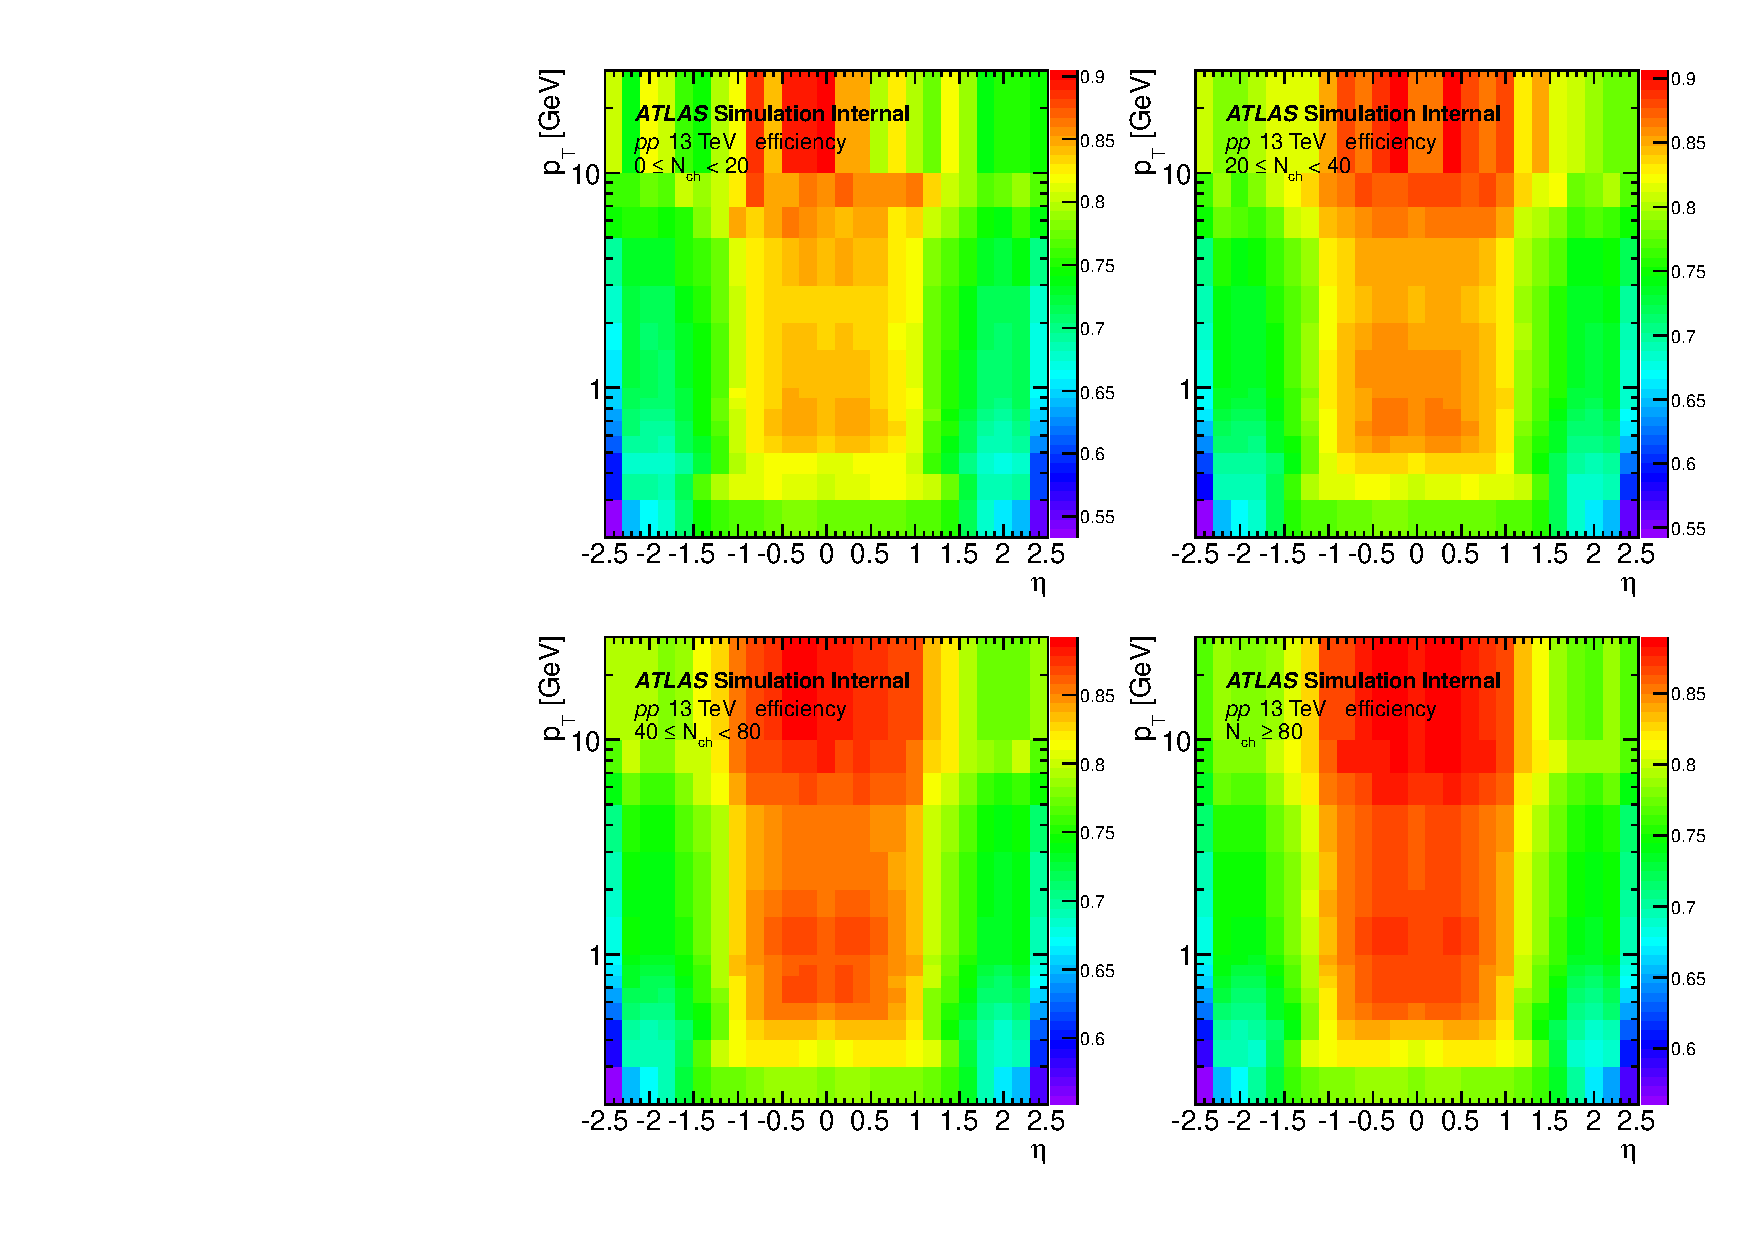
\includegraphics[width=1.\linewidth]{figs/sec_evtSlc/trkEff_pp13_eff_2D.pdf}
\caption{Tracking efficiency $\epsilon(\eta,p_{T})$. Different panels are for different $N_{ch}$ ranges, where different $z_{vtx}$ ranges have been merged.}
\label{fig:trkEff_pp13_eff_2D}
\end{figure}

The merged tracking efficiency is shown in Fig.~\ref{fig:trkEff_pp13_eff_2D}, where four panels are for four different $N_{ch}$ ranges. The boundaries of ranges are chosen to make each range have enough statistics for the efficiency measurement. The efficiency is higher in high multiplicity. These efficiency maps are applied in this analysis, where linear interpolation is used to obtain the more precise efficiency when $p_{\text{T}}$ or $\eta$ are not in the bin center. The $c_{2}{4}$ are compared with using tracking efficiency from previous cumulant measurement and the results are consistent.

\begin{figure}[H]
\centering
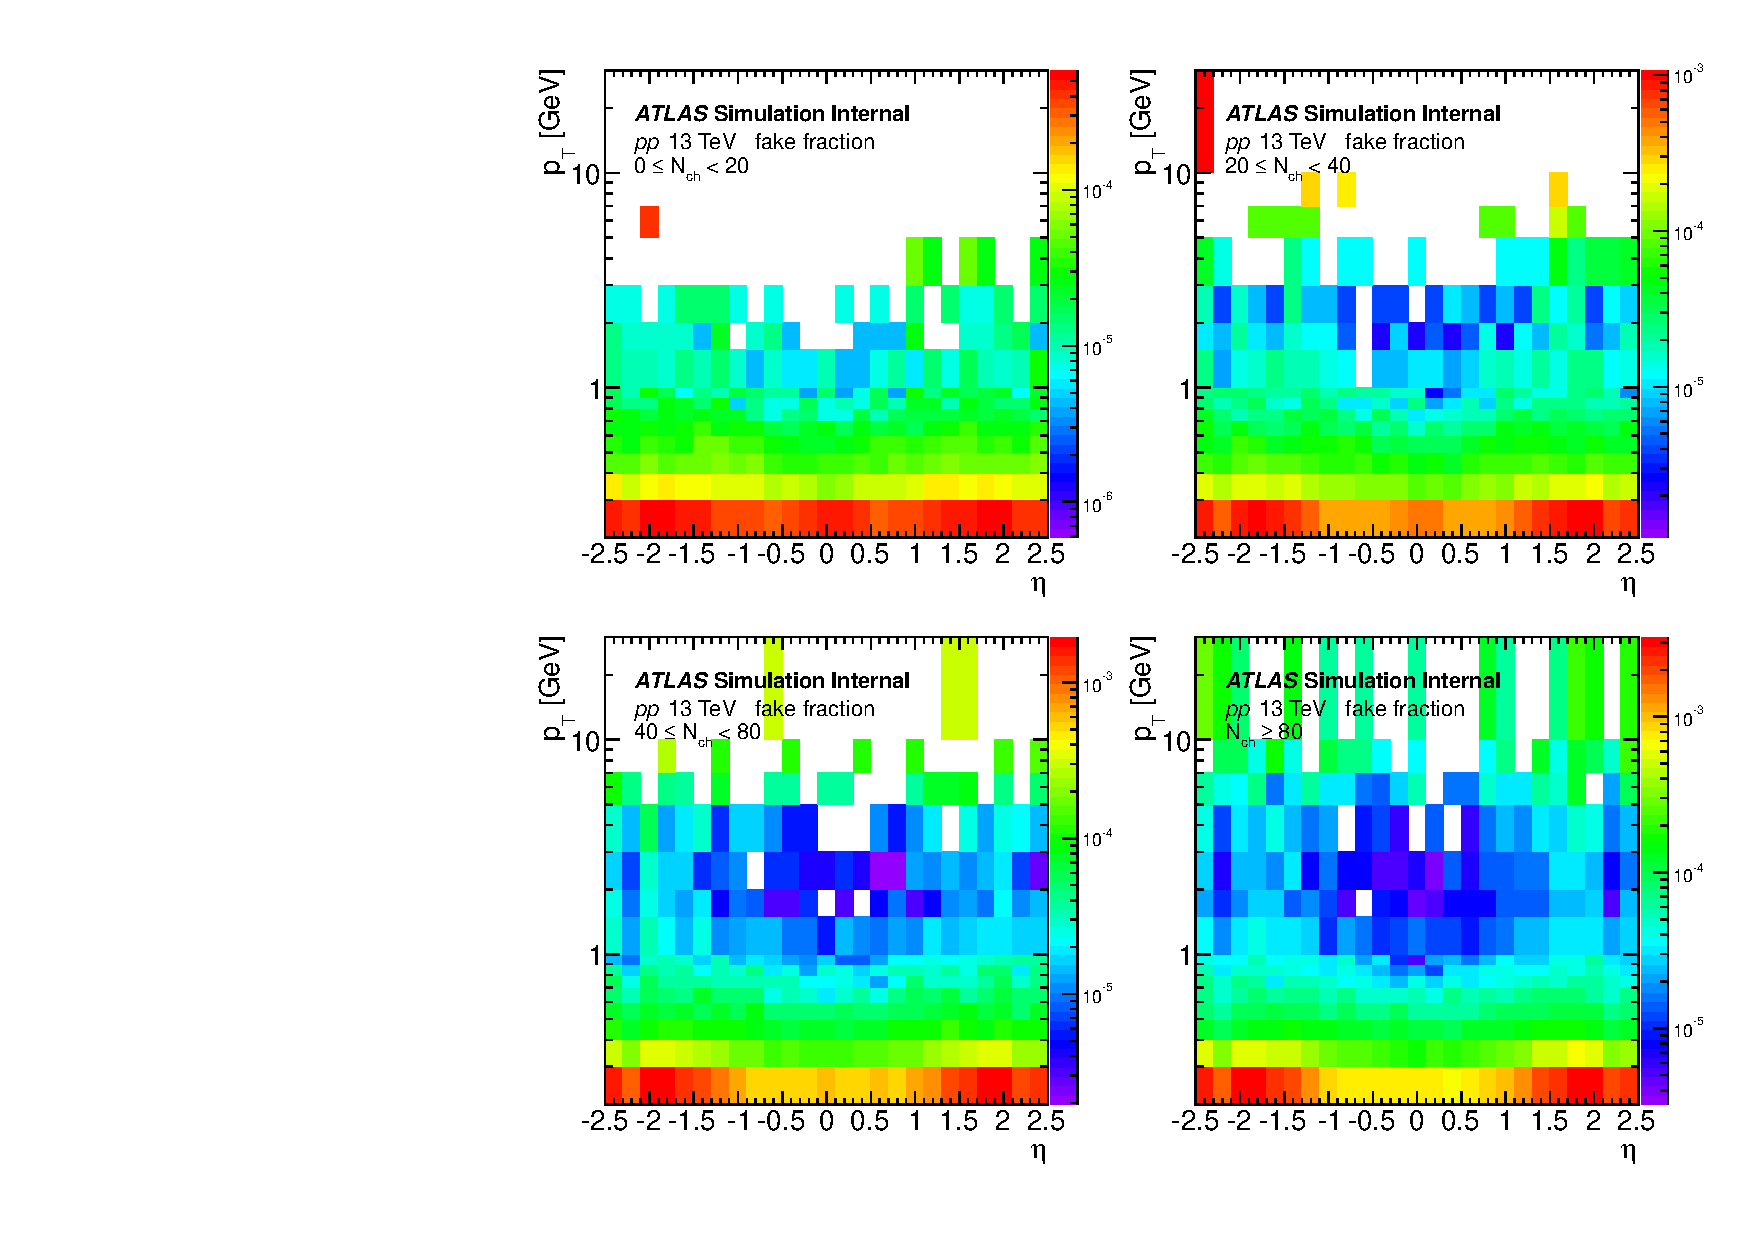
\includegraphics[width=1.\linewidth]{figs/sec_evtSlc/trkEff_pp13_fak_2D.pdf}
\caption{Fake fraction $f(\eta,p_{T})$. Different panels are for different $N_{ch}$ ranges, where different $z_{vtx}$ ranges have been merged.}
\label{fig:trkEff_pp13_fak_2D}
\end{figure}

The merged fake fraction is shown in Fig.~\ref{fig:trkEff_pp13_fak_2D}, where four panels are for four different $N_{ch}$ ranges. Since the maximum fake fraction is smaller than the level of $0.1\%$, even for the lowest $p_{T}$, we will not apply this additional correction in the data analysis.

In the systematics section we will test the stability of the results by varying the tracking efficiency.

Appendix~\ref{sec:appdx} summarizes many detailed monitoring plots for this PYTHIA sample.



\subsubsection{Tracking validation for run 305359, 309314 and 309346}
When producing the GRL for the low-$\mu$ $pp$ runs in 2016, three runs are tagged with following issues:
\begin{itemize}
\item Run 305359: \verb|BTAG_BLAYER_SERIOUS_PROBLEM|
\item Run 309314: \verb|ID_BS_RUNAVERAGE|
\item Run 309346: \verb|ID_BS_RUNAVERAGE|
\end{itemize}
where in run 305359, the IBL detector is absent while in the other two runs, there is no constrain on the beam spot position at the trigger level. (The offline reconstruction DOES impose the beam spot constraint in all runs.) When beam spot is constraint, fluctuation of rate of HMT triggers has been observed, due to online reconstruction issues.

The purpose of this section is to validate the basic tracking quantities in these three runs, to check whether IBL and beam spot can have an impact on the results. Run 310216 is used as a reference for comparison. All the events are required to pass the MB trigger \verb|HLT_mb_sptrk| and the track selection is identical to the $pp$ analysis.

\begin{figure}[H]
\centering
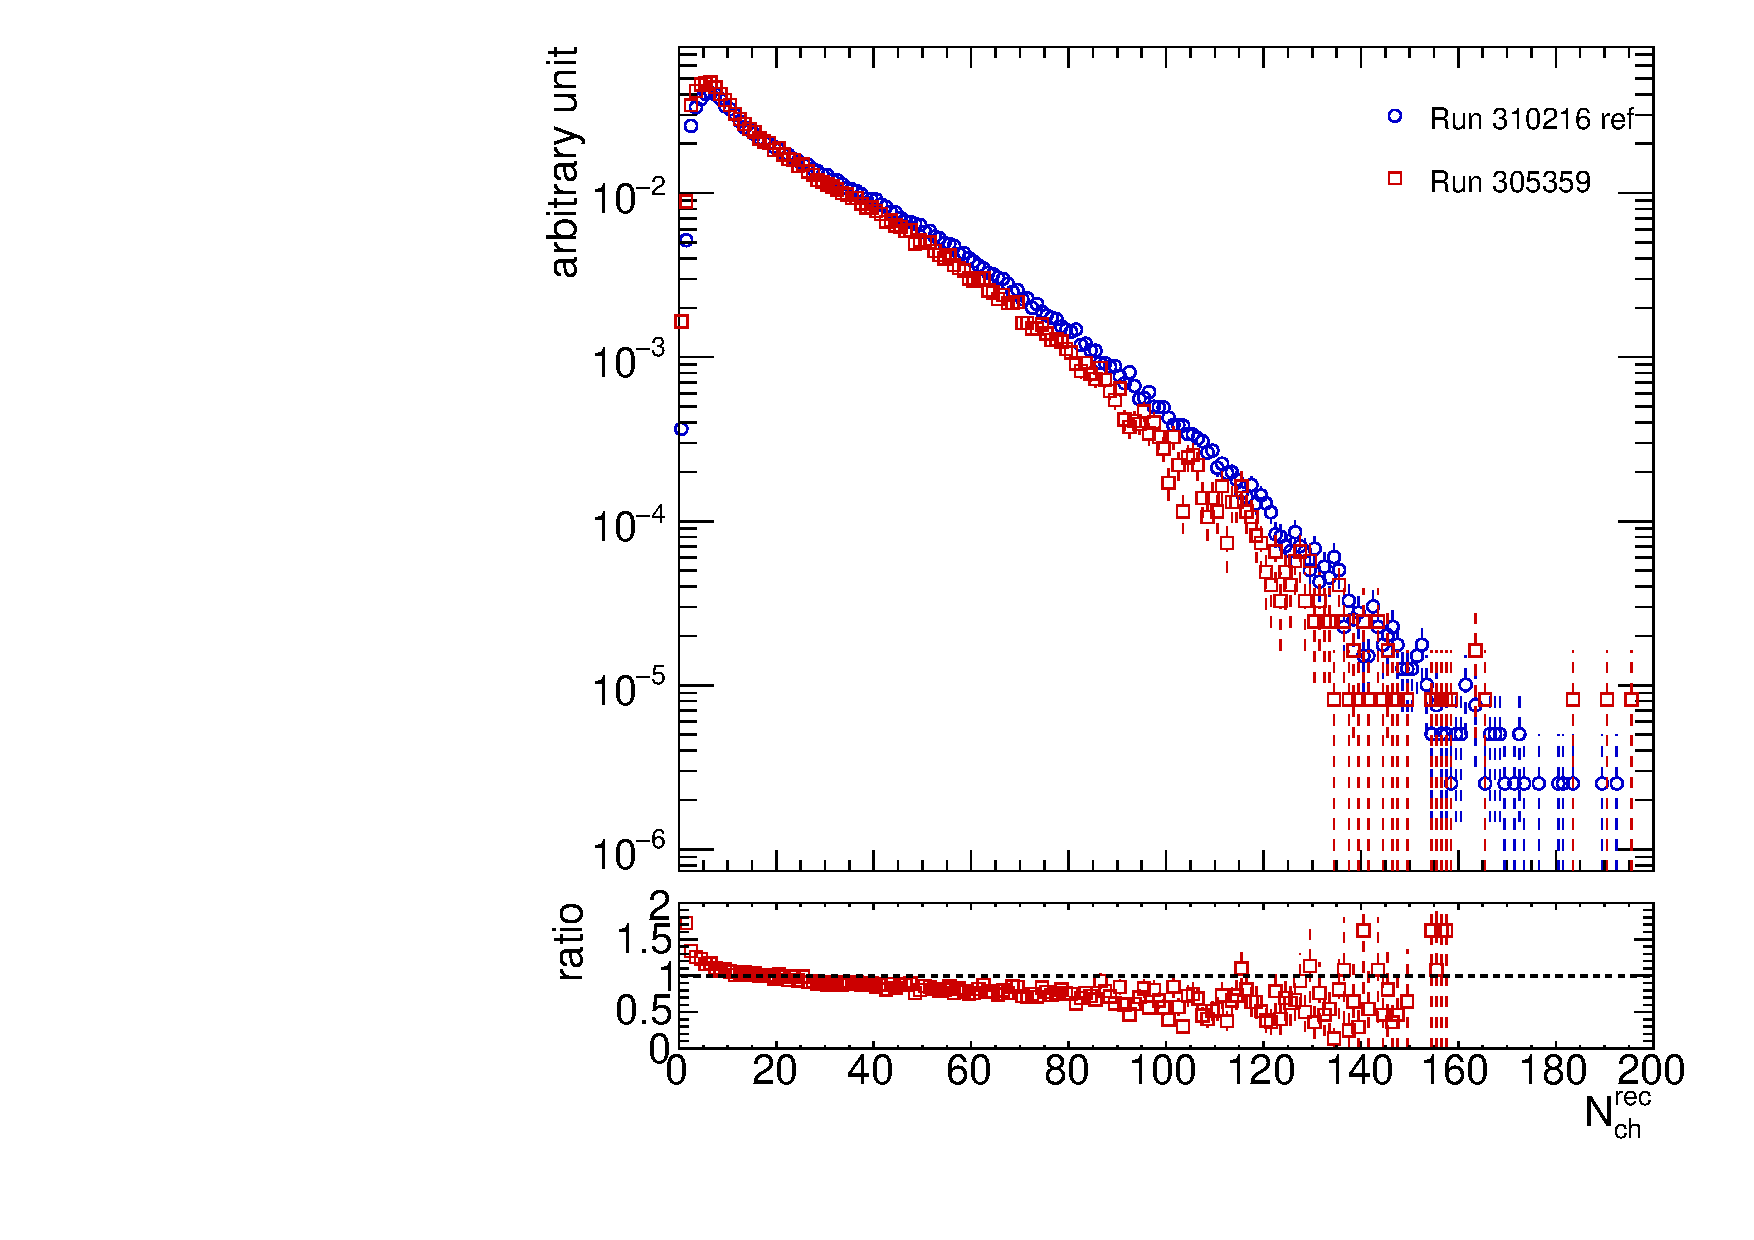
\includegraphics[width=0.45\linewidth]{figs/sec_evtSlc/GRLpp2016/305359_dis_nTrk.pdf}
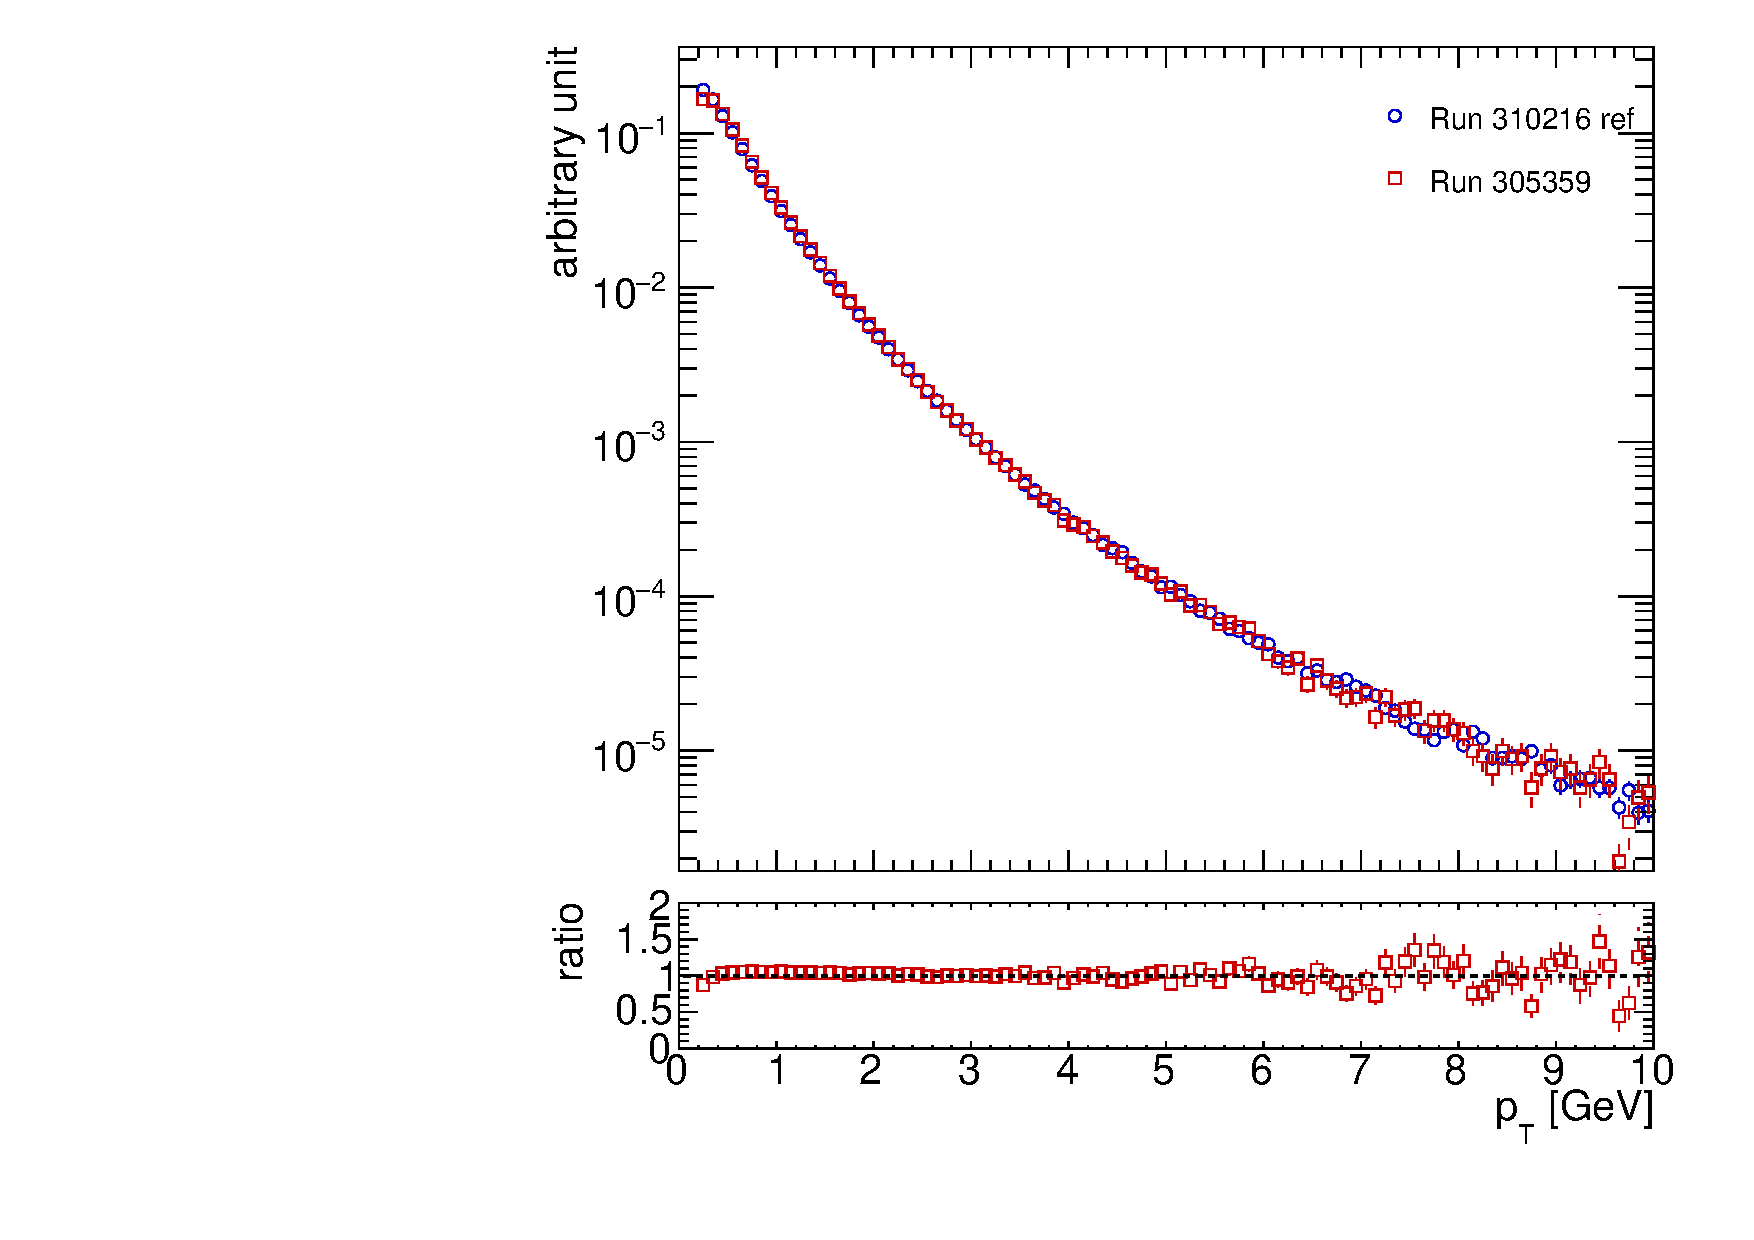
\includegraphics[width=0.45\linewidth]{figs/sec_evtSlc/GRLpp2016/305359_dis_pt.pdf}
\caption{Distribution of number of offline reconstructed tracks and $p_{\text{T}}$ spectrum: a comparison between run 305359 and run 310216.}
\label{fig:GRLpp2016_305359_nTrk_pt}
\end{figure}
Fig.~\ref{fig:GRLpp2016_305359_nTrk_pt} shows the comparison of number of reconstructed tracks distribution and $p_{\text{T}}$ spectrum, between run 305359 and 310216. The mean value of number of tracks is slightly smaller in 305359 than 310216. This is probably due to that the IBL is absent in 305359, and same cut on number of Pixel hits will reject slightly more events in this run. Meanwhile, the $p_{\text{T}}$ spectrums are consistent between the two runs, except for the lowest $p_{\text{T}}$ region, where again it is due to the absence of IBL detector, thus the tracking reconstruction has a poorer efficiency in the lowest $p_{\text{T}}$ region. We will come back to this behavior again once we show the comparison of Run 1 and Run 2 $p$+Pb tracking efficiency.

\begin{figure}[H]
\centering
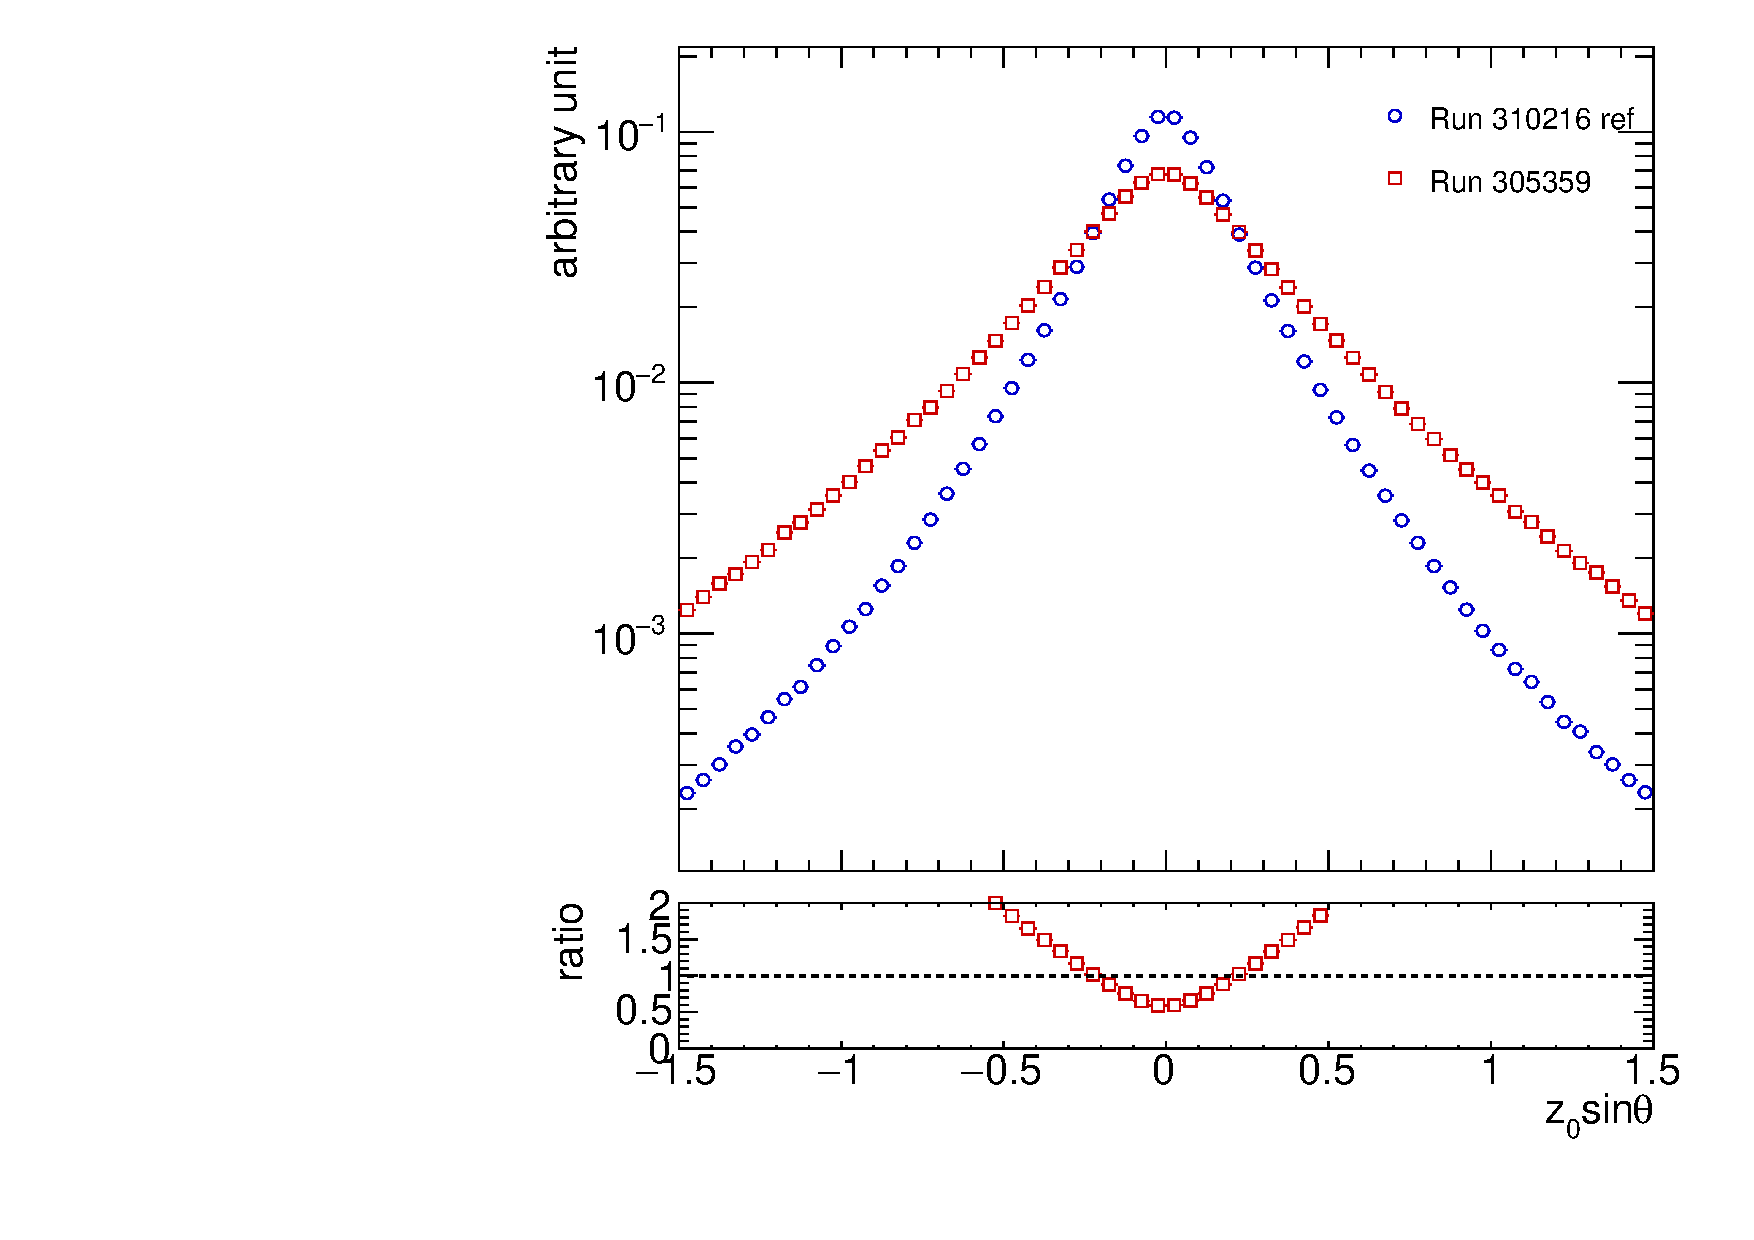
\includegraphics[width=0.45\linewidth]{figs/sec_evtSlc/GRLpp2016/305359_dis_z0.pdf}
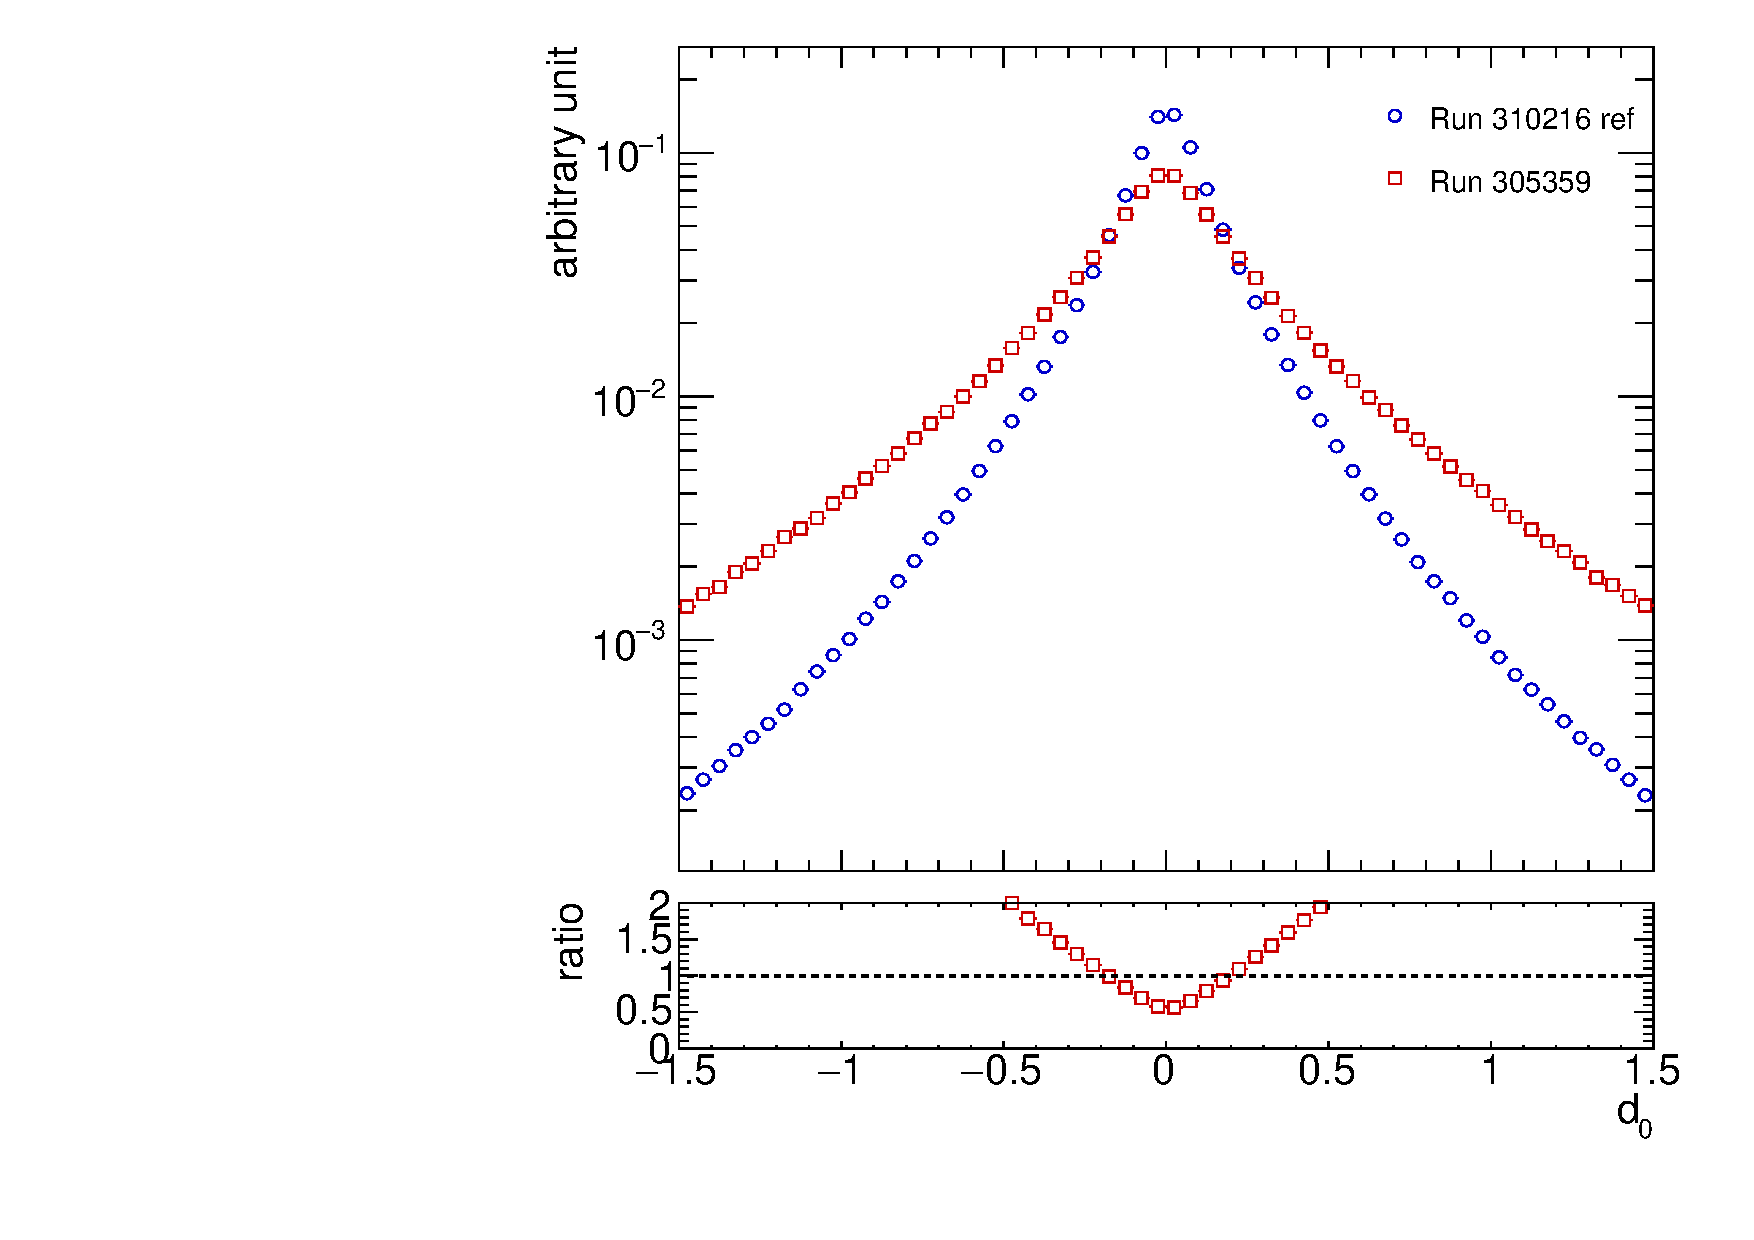
\includegraphics[width=0.45\linewidth]{figs/sec_evtSlc/GRLpp2016/305359_dis_d0.pdf}
\caption{Distribution of $z_{0}\text{sin}\theta$ and $d_{0}$ of reconstructed tracks: a comparison between run 305359 and run 310216.}
\label{fig:GRLpp2016_305359_z0_d0}
\end{figure}
Fig.~\ref{fig:GRLpp2016_305359_z0_d0} shows the comparison of $z_{0}\text{sin}\theta$ and $d_{0}$ distribution of reconstructed tracks, between run 305359 and 310216. Both $z_{0}$ and $d_{0}$ distributions are much wider when IBL is absent. The default tracking pointing cut is at 1.5 mm, which will result in different tracks because of the different $z_{0}$ and $d_{0}$ distribution.

\begin{figure}[H]
\centering
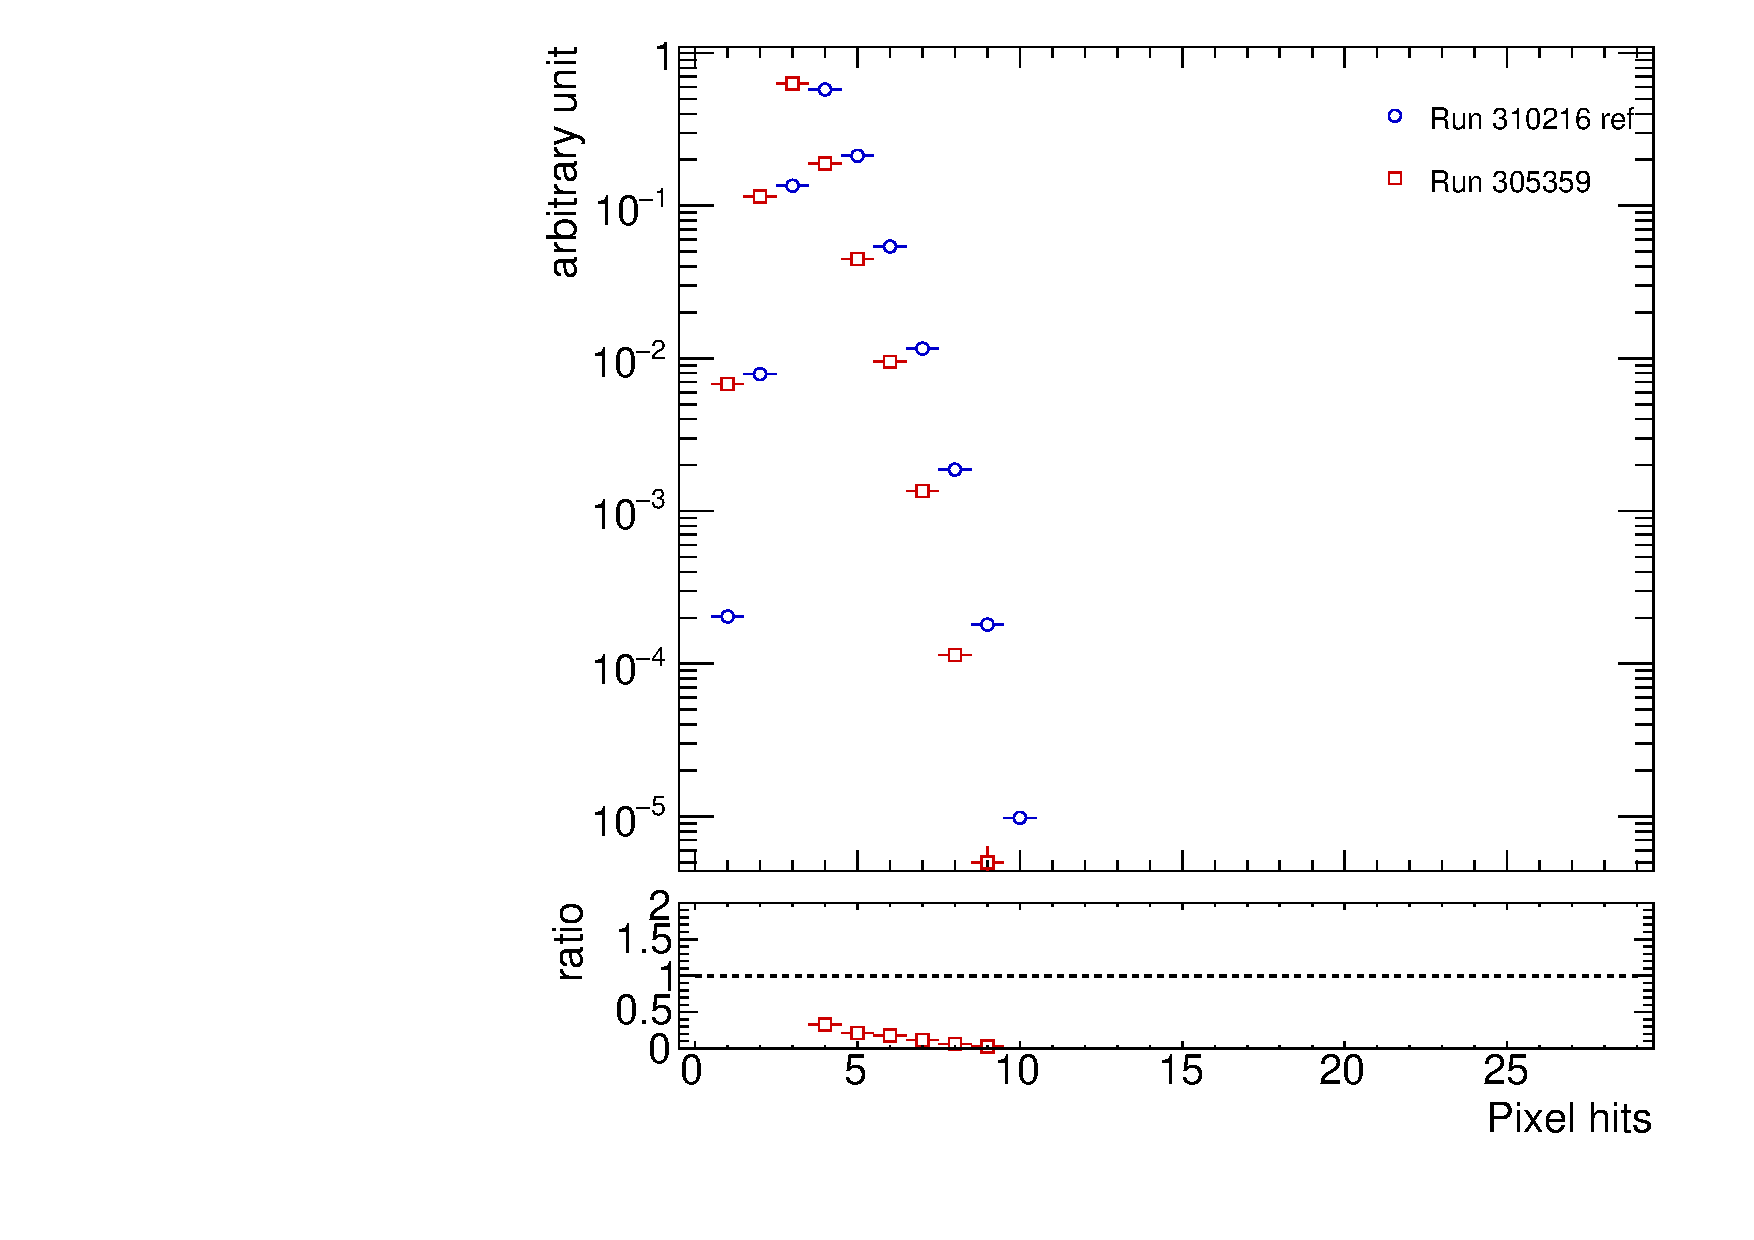
\includegraphics[width=0.45\linewidth]{figs/sec_evtSlc/GRLpp2016/305359_dis_pixHit.pdf}
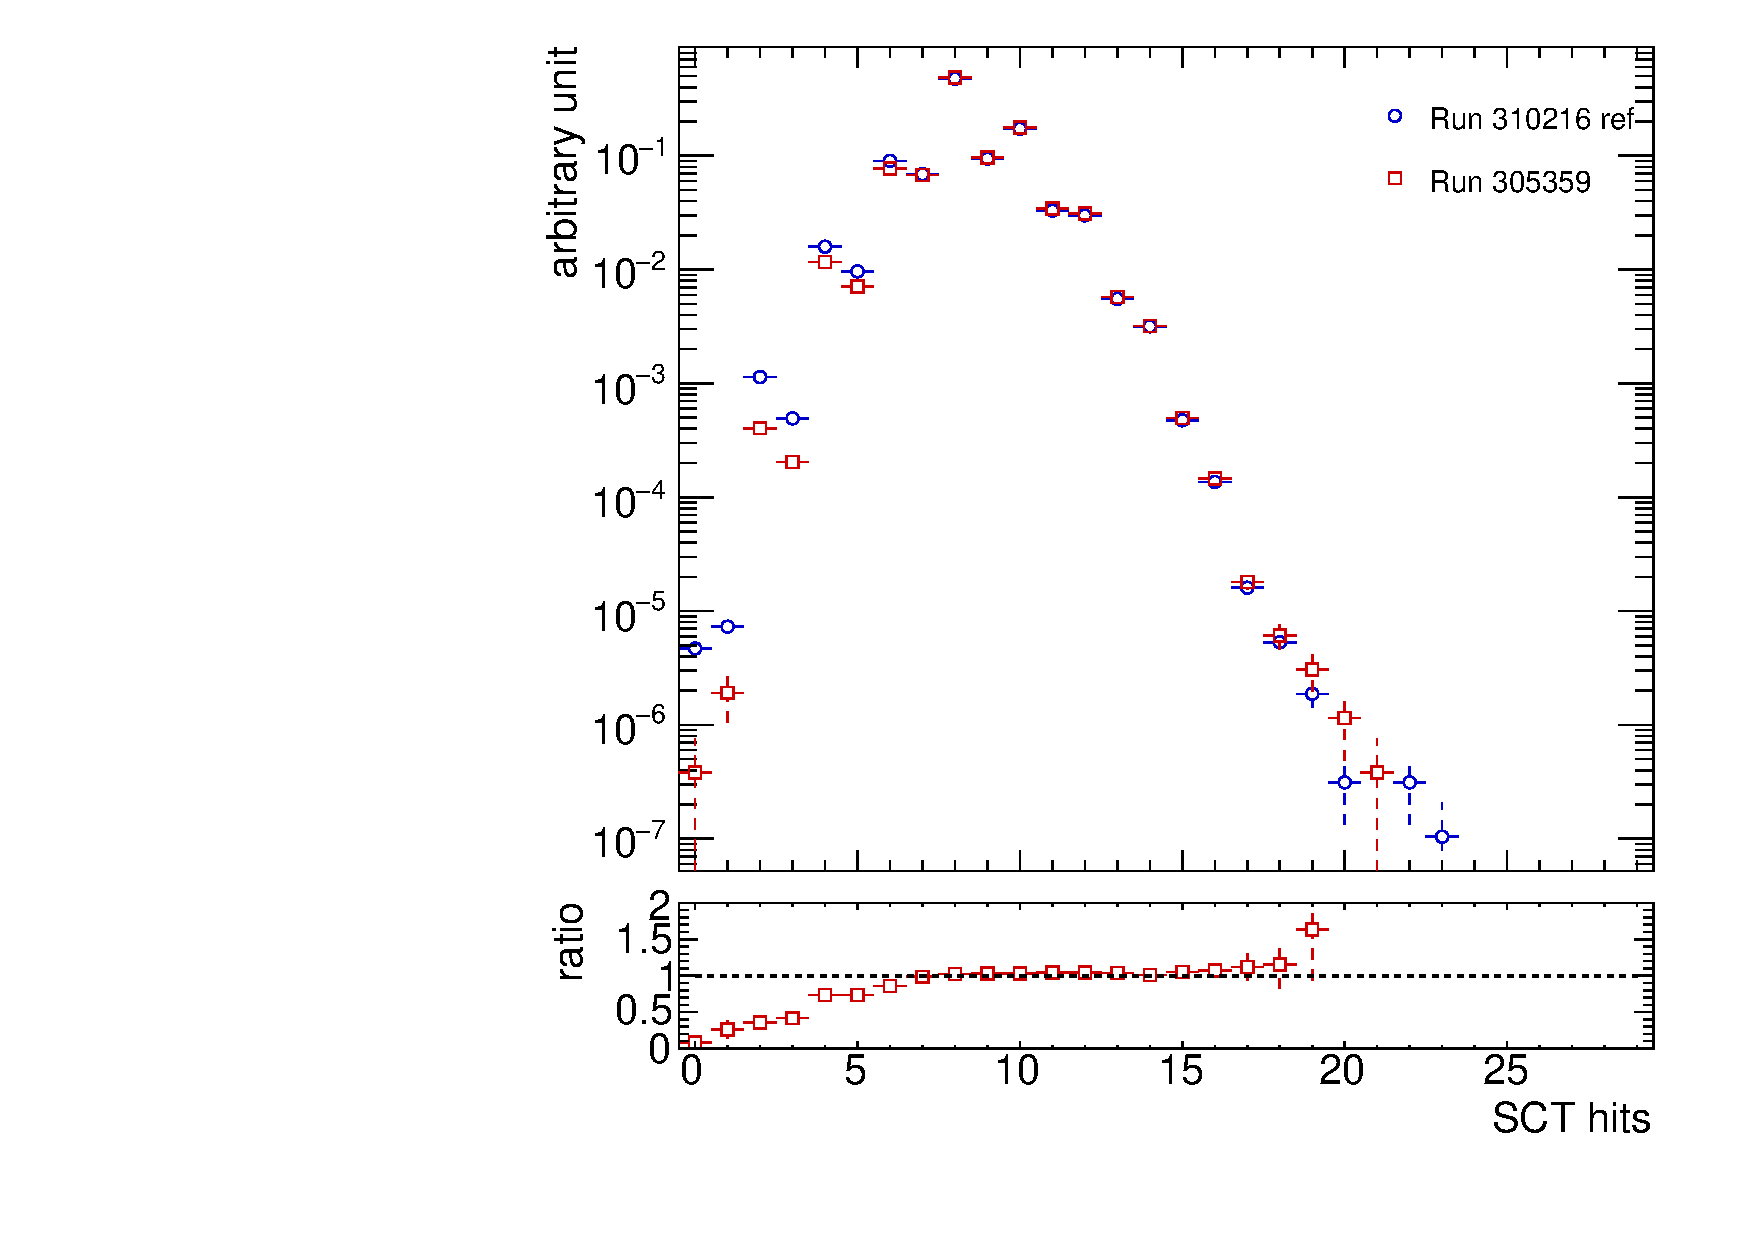
\includegraphics[width=0.45\linewidth]{figs/sec_evtSlc/GRLpp2016/305359_dis_sctHit.pdf}
\caption{Distribution of number of Pixel and SCT hits of reconstructed tracks: a comparison between run 305359 and run 310216.}
\label{fig:GRLpp2016_305359_pixHit_sctHit}
\end{figure}
Fig.~\ref{fig:GRLpp2016_305359_pixHit_sctHit} shows the comparison of number of Pixel and SCT hits, between run 305359 and 310216. Due to absence of IBL, the number of Pixel hits in run 305359 is shifted by 1 compared with 310216. The number of SCT hits are consistent between the two runs, above the default track selection cut.

\begin{figure}[H]
\centering
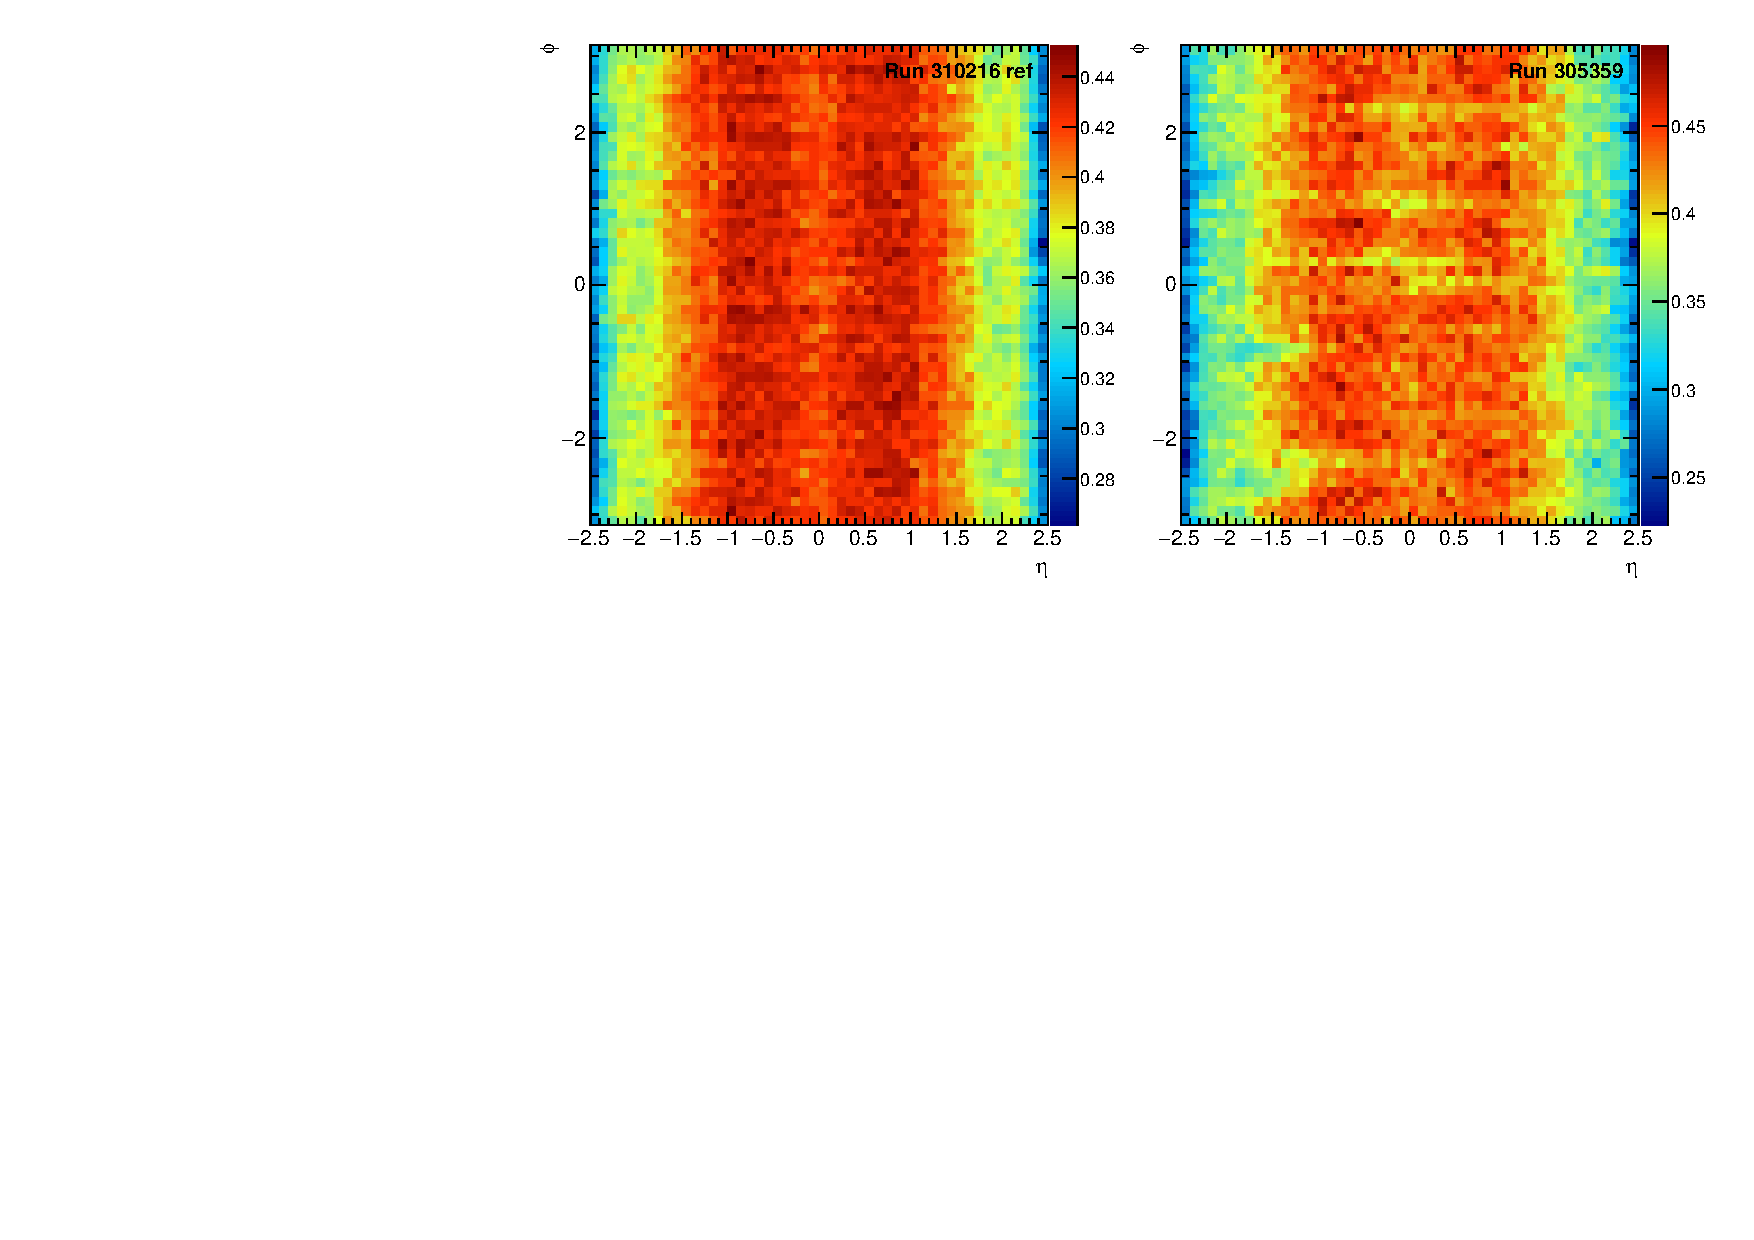
\includegraphics[width=0.9\linewidth]{figs/sec_evtSlc/GRLpp2016/305359_crr_eta_phi.pdf}
\caption{2D map of raw $\eta$-$\phi$ distribution: a comparison between run 305359 and run 310216.}
\label{fig:GRLpp2016_305359_eta_phi}
\end{figure}
Finally, fig.~\ref{fig:GRLpp2016_305359_eta_phi} shows the 2D map of raw $\eta$-$\phi$ distribution. "raw" means the tracks are not weighted by tracking efficiency. The distribution is much more uniform in run 310216 than 305359.

As a conclusion, because of the absence of IBL, $z_{0}$, $d_{0}$ and $\eta$-$\phi$ distributions are quite different between run 310216 and 305359. In principle, most of the differences can be covered by a dedicated Monte-Carlo sample with special detector setup for the run 305359. However, after discussion with the experts who prepared the GRL, we decide not to include run 305359, which only contributes to less than 10$\%$ of the total statistics.

\begin{figure}[H]
\centering
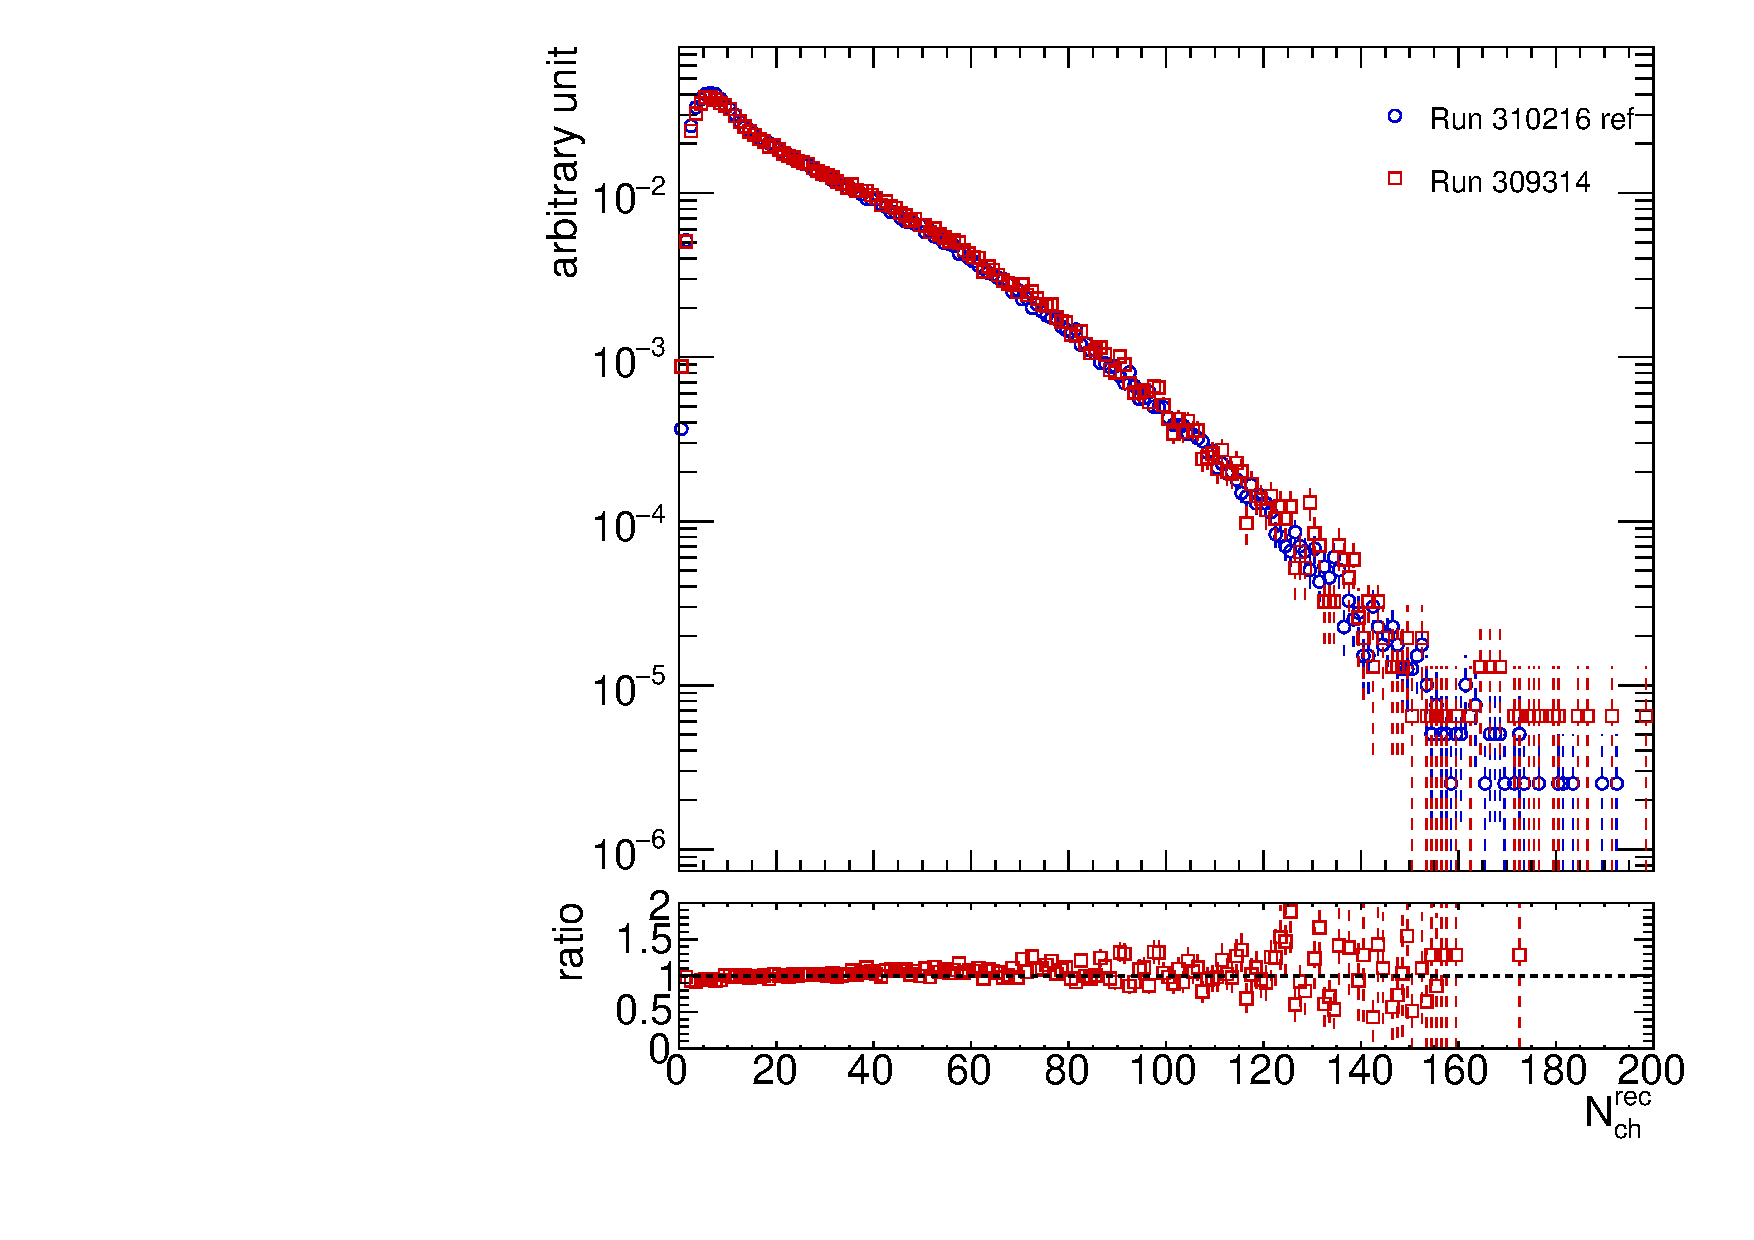
\includegraphics[width=0.45\linewidth]{figs/sec_evtSlc/GRLpp2016/309314_dis_nTrk.pdf}
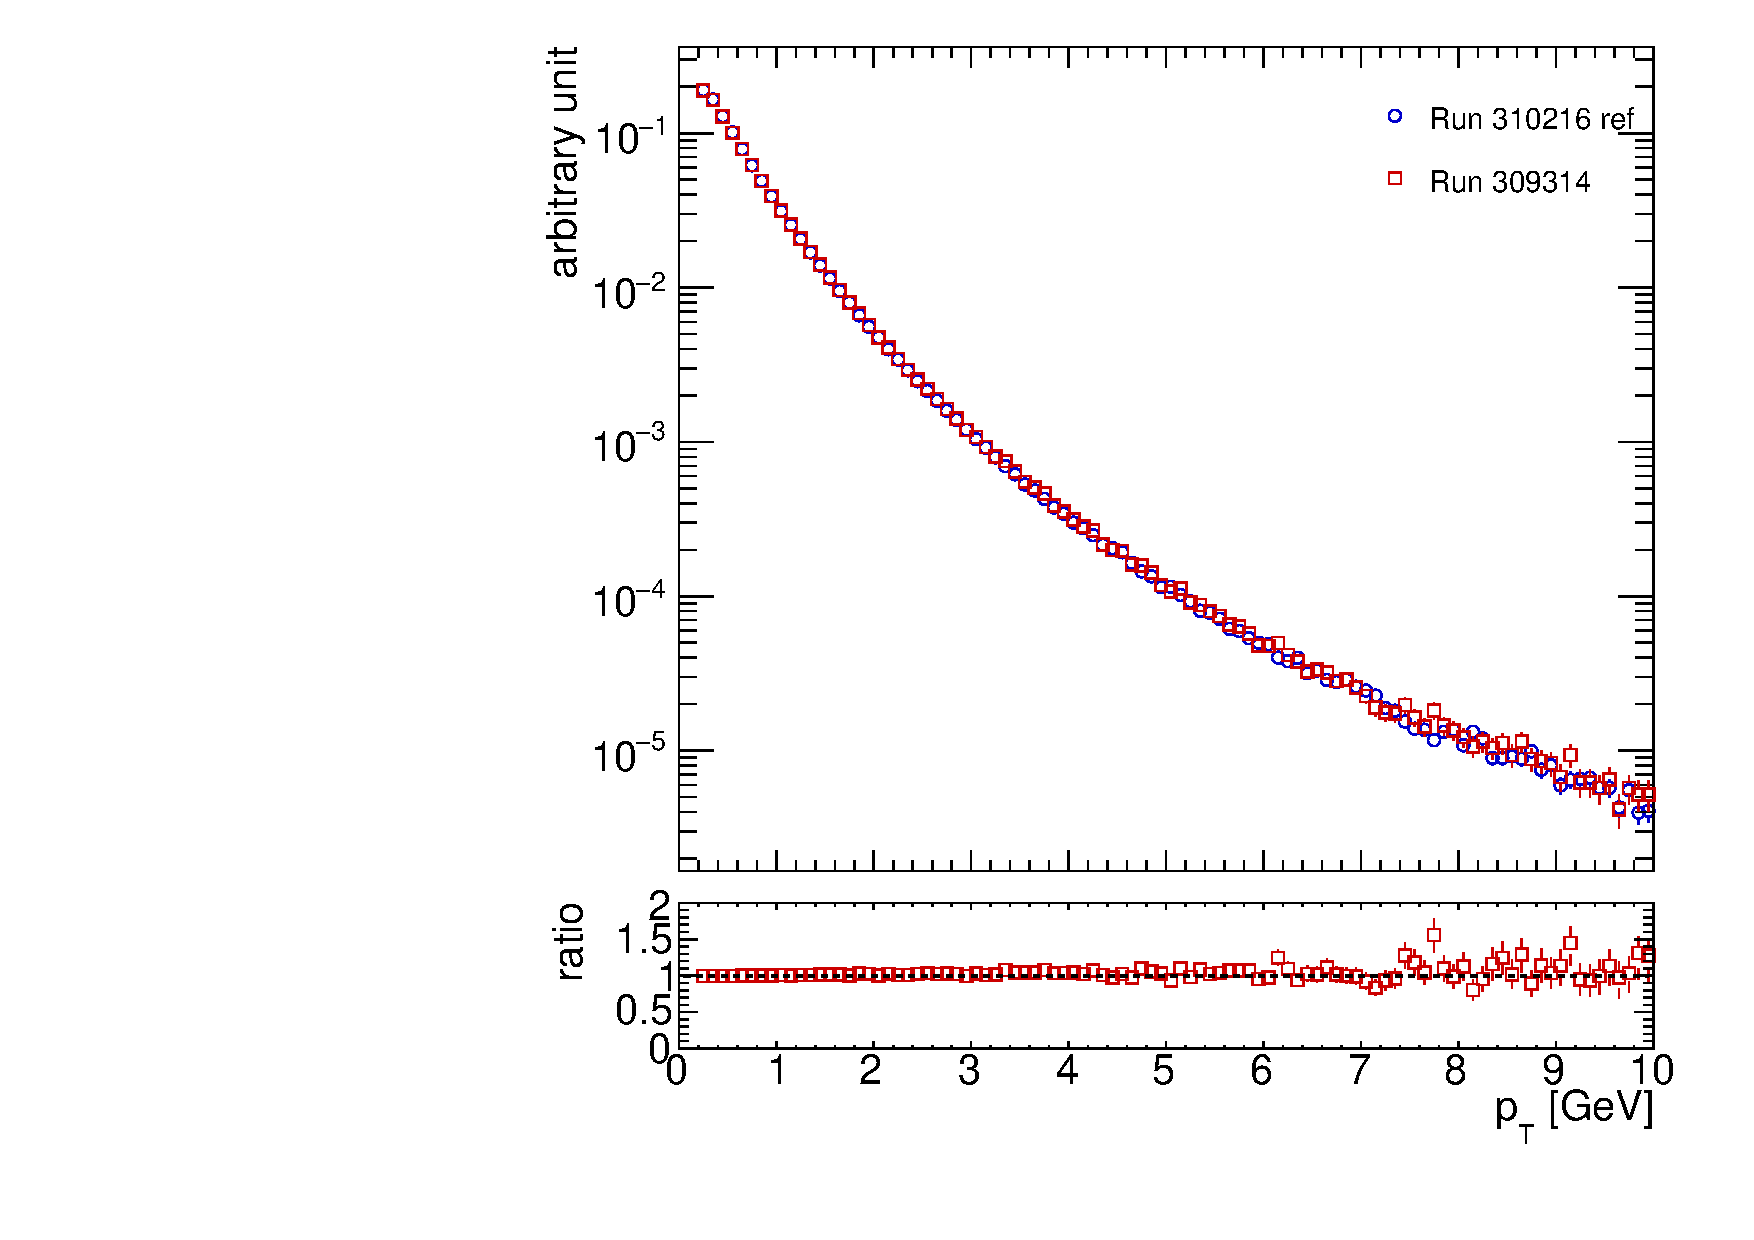
\includegraphics[width=0.45\linewidth]{figs/sec_evtSlc/GRLpp2016/309314_dis_pt.pdf}
\caption{Distribution of number of offline reconstructed tracks and $p_{\text{T}}$ spectrum: a comparison between run 309314 and run 310216.}
\label{fig:GRLpp2016_309314_nTrk_pt}
\end{figure}
The rest two runs are tagged with the error \verb|ID_BS_RUNAVERAGE|, since the beam spot position is not constraint. In the following we will demonstrate that tracking quantities will be consistent without beam spot constraint. Fig.~\ref{fig:GRLpp2016_309314_nTrk_pt} shows the comparison of number of reconstructed tracks distribution and $p_{\text{T}}$ spectrum, between run 309314 and 310216. The ratios show that they are very consistent.

\begin{figure}[H]
\centering
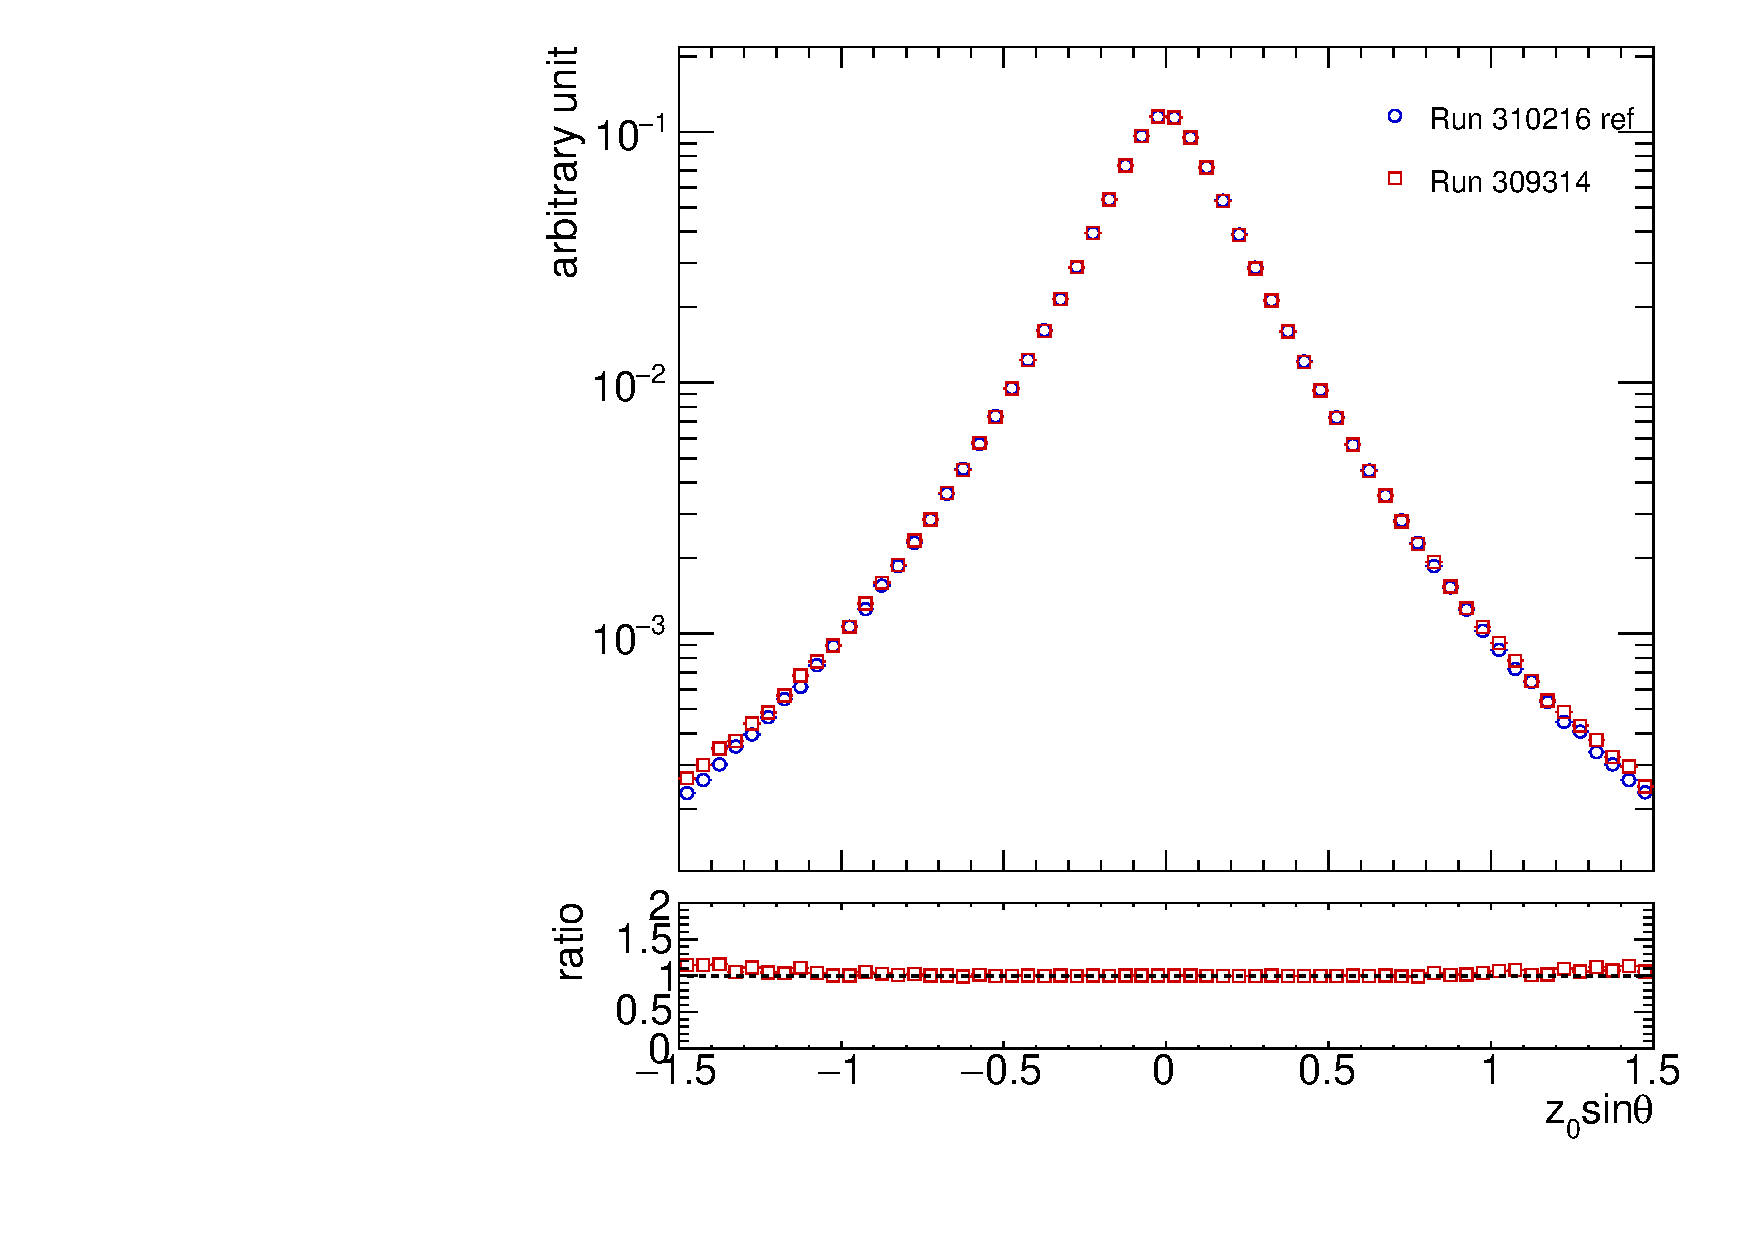
\includegraphics[width=0.45\linewidth]{figs/sec_evtSlc/GRLpp2016/309314_dis_z0.pdf}
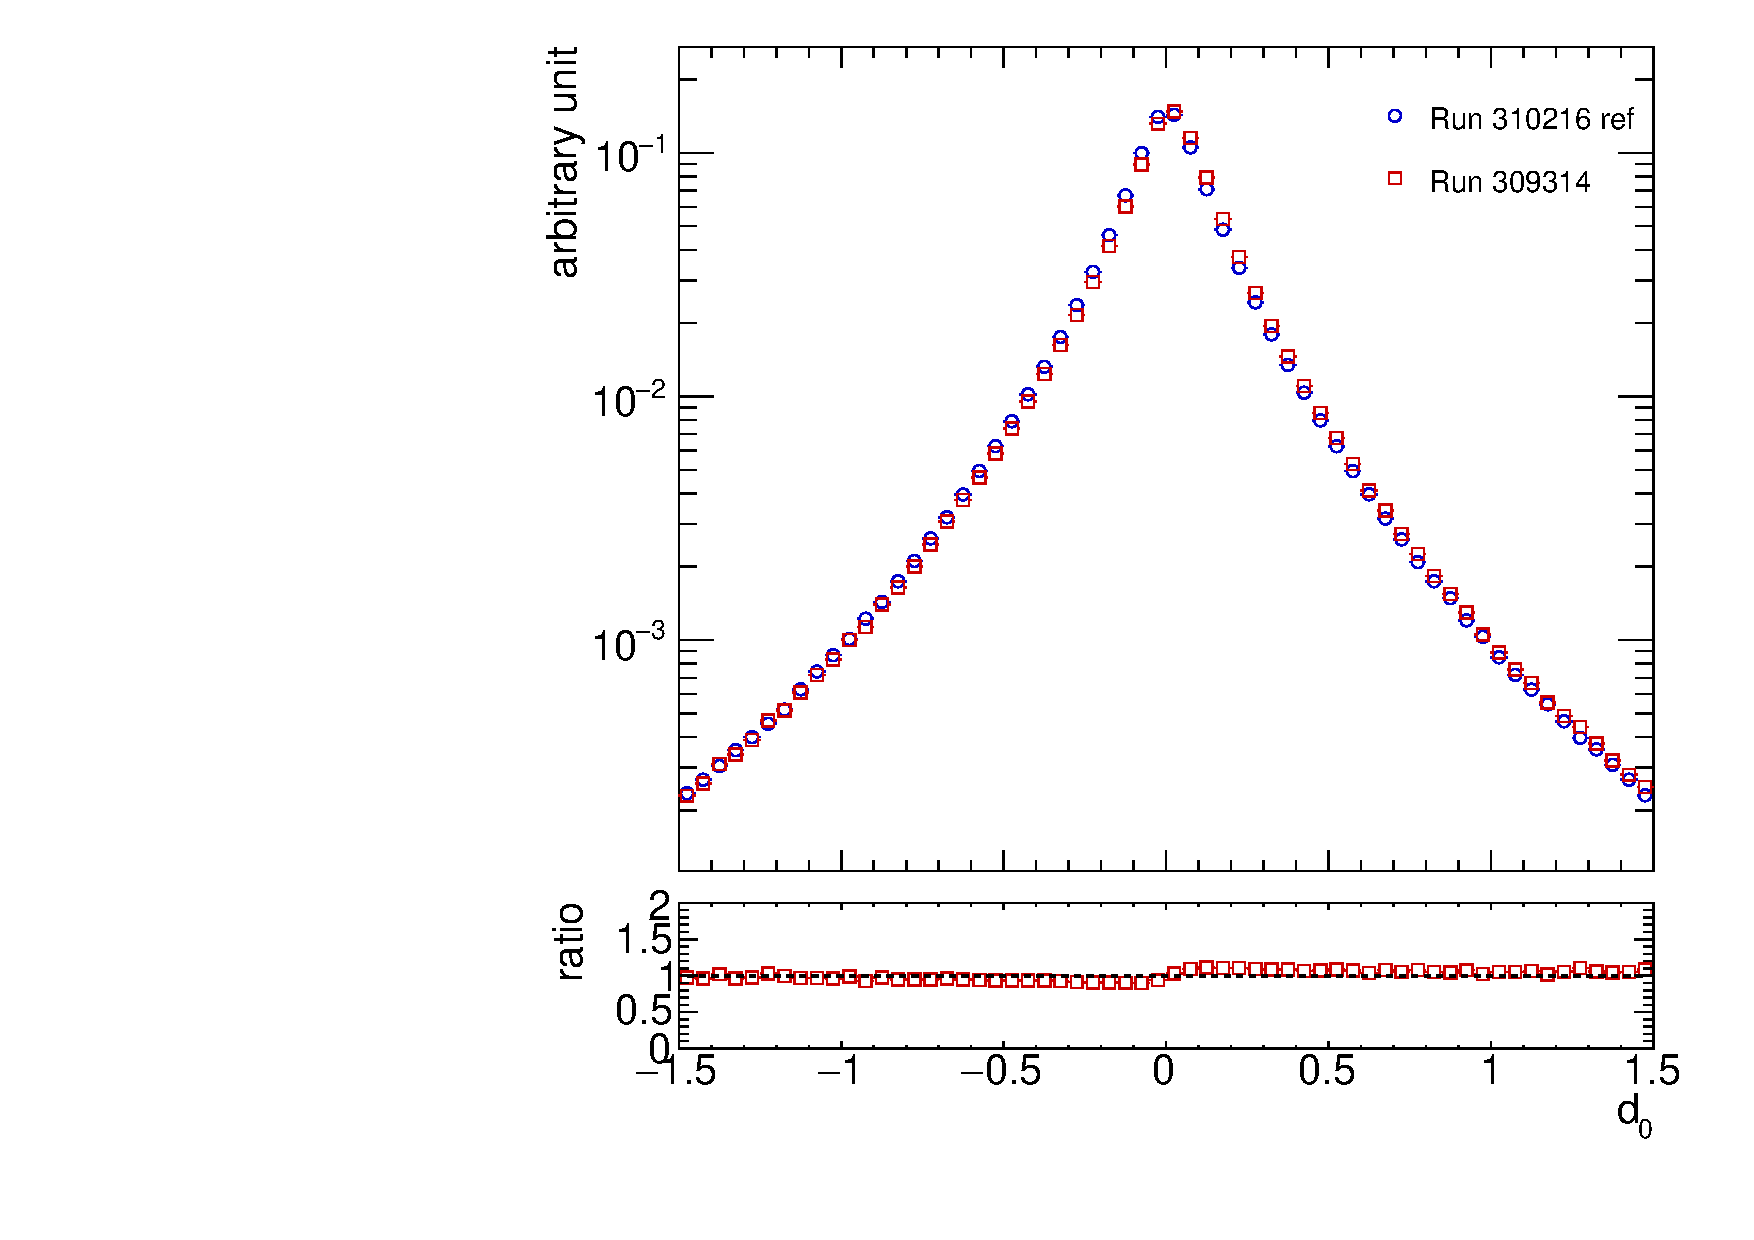
\includegraphics[width=0.45\linewidth]{figs/sec_evtSlc/GRLpp2016/309314_dis_d0.pdf}
\caption{Distribution of $z_{0}\text{sin}\theta$ and $d_{0}$ of reconstructed tracks: a comparison between run 309314 and run 310216.}
\label{fig:GRLpp2016_309314_z0_d0}
\end{figure}
Fig.~\ref{fig:GRLpp2016_309314_z0_d0} shows the comparison of $z_{0}\text{sin}\theta$ and $d_{0}$ distribution of reconstructed tracks, between run 309314 and 310216. They are very consistent.

\begin{figure}[H]
\centering
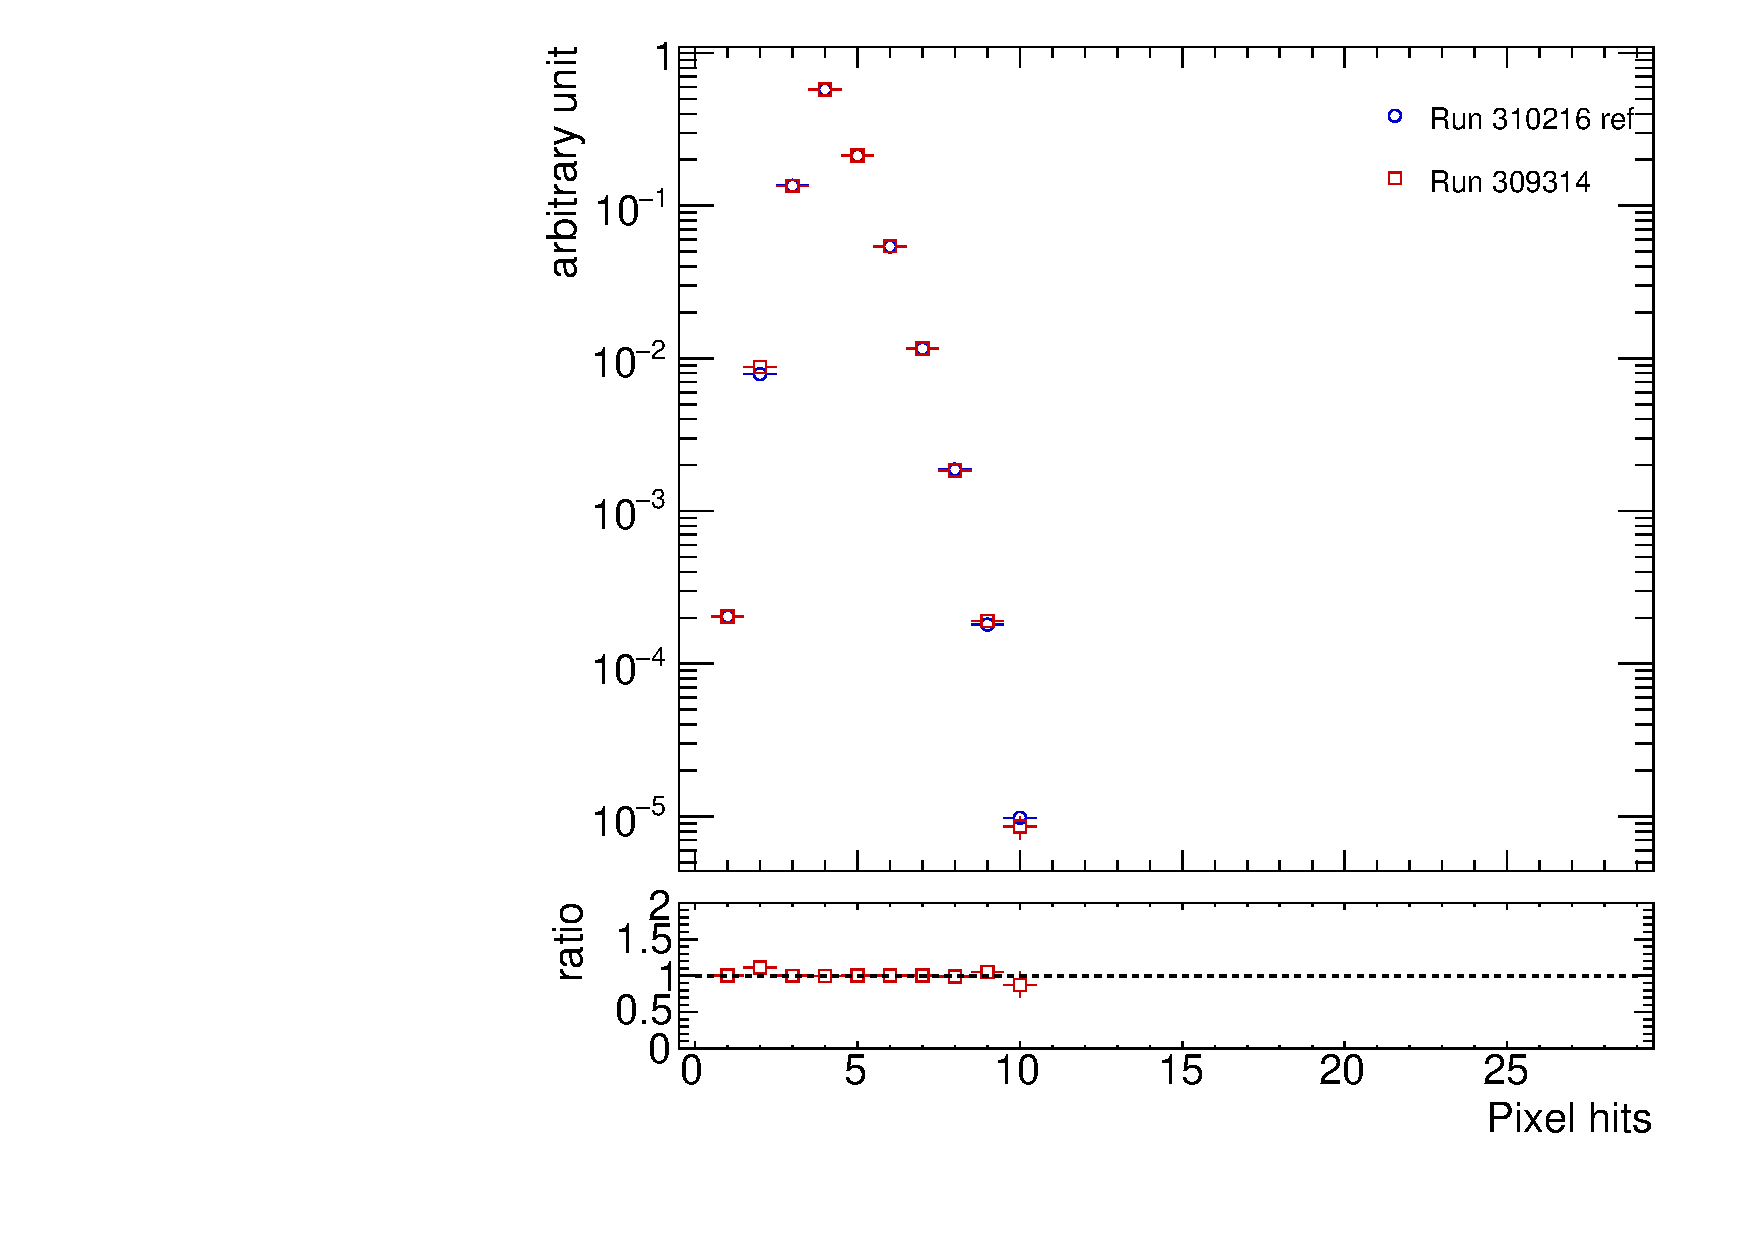
\includegraphics[width=0.45\linewidth]{figs/sec_evtSlc/GRLpp2016/309314_dis_pixHit.pdf}
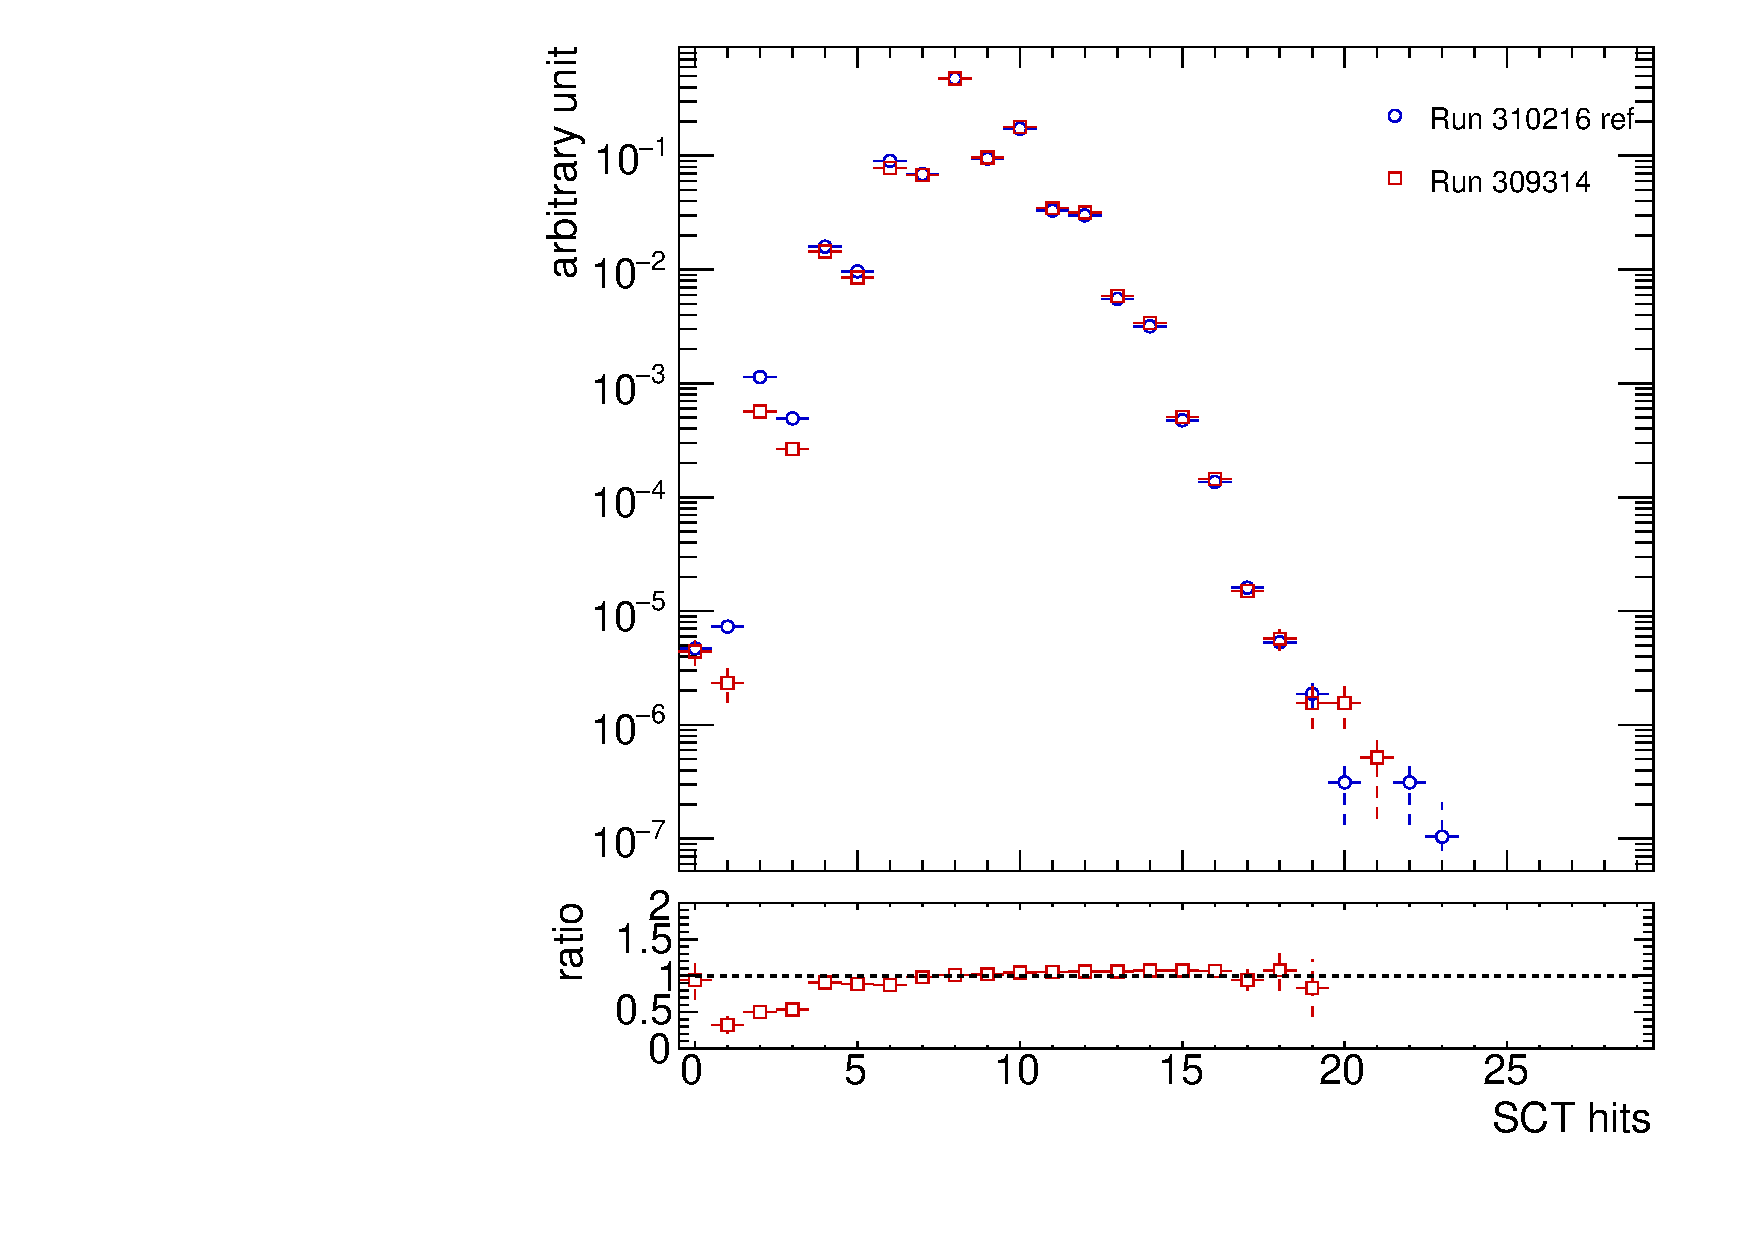
\includegraphics[width=0.45\linewidth]{figs/sec_evtSlc/GRLpp2016/309314_dis_sctHit.pdf}
\caption{Distribution of number of Pixel and SCT hits of reconstructed tracks: a comparison between run 309314 and run 310216.}
\label{fig:GRLpp2016_309314_pixHit_sctHit}
\end{figure}
Fig.~\ref{fig:GRLpp2016_309314_pixHit_sctHit} shows the comparison of number of Pixel and SCT hits, between run 309314 and 310216. They are very consistent.

\begin{figure}[H]
\centering
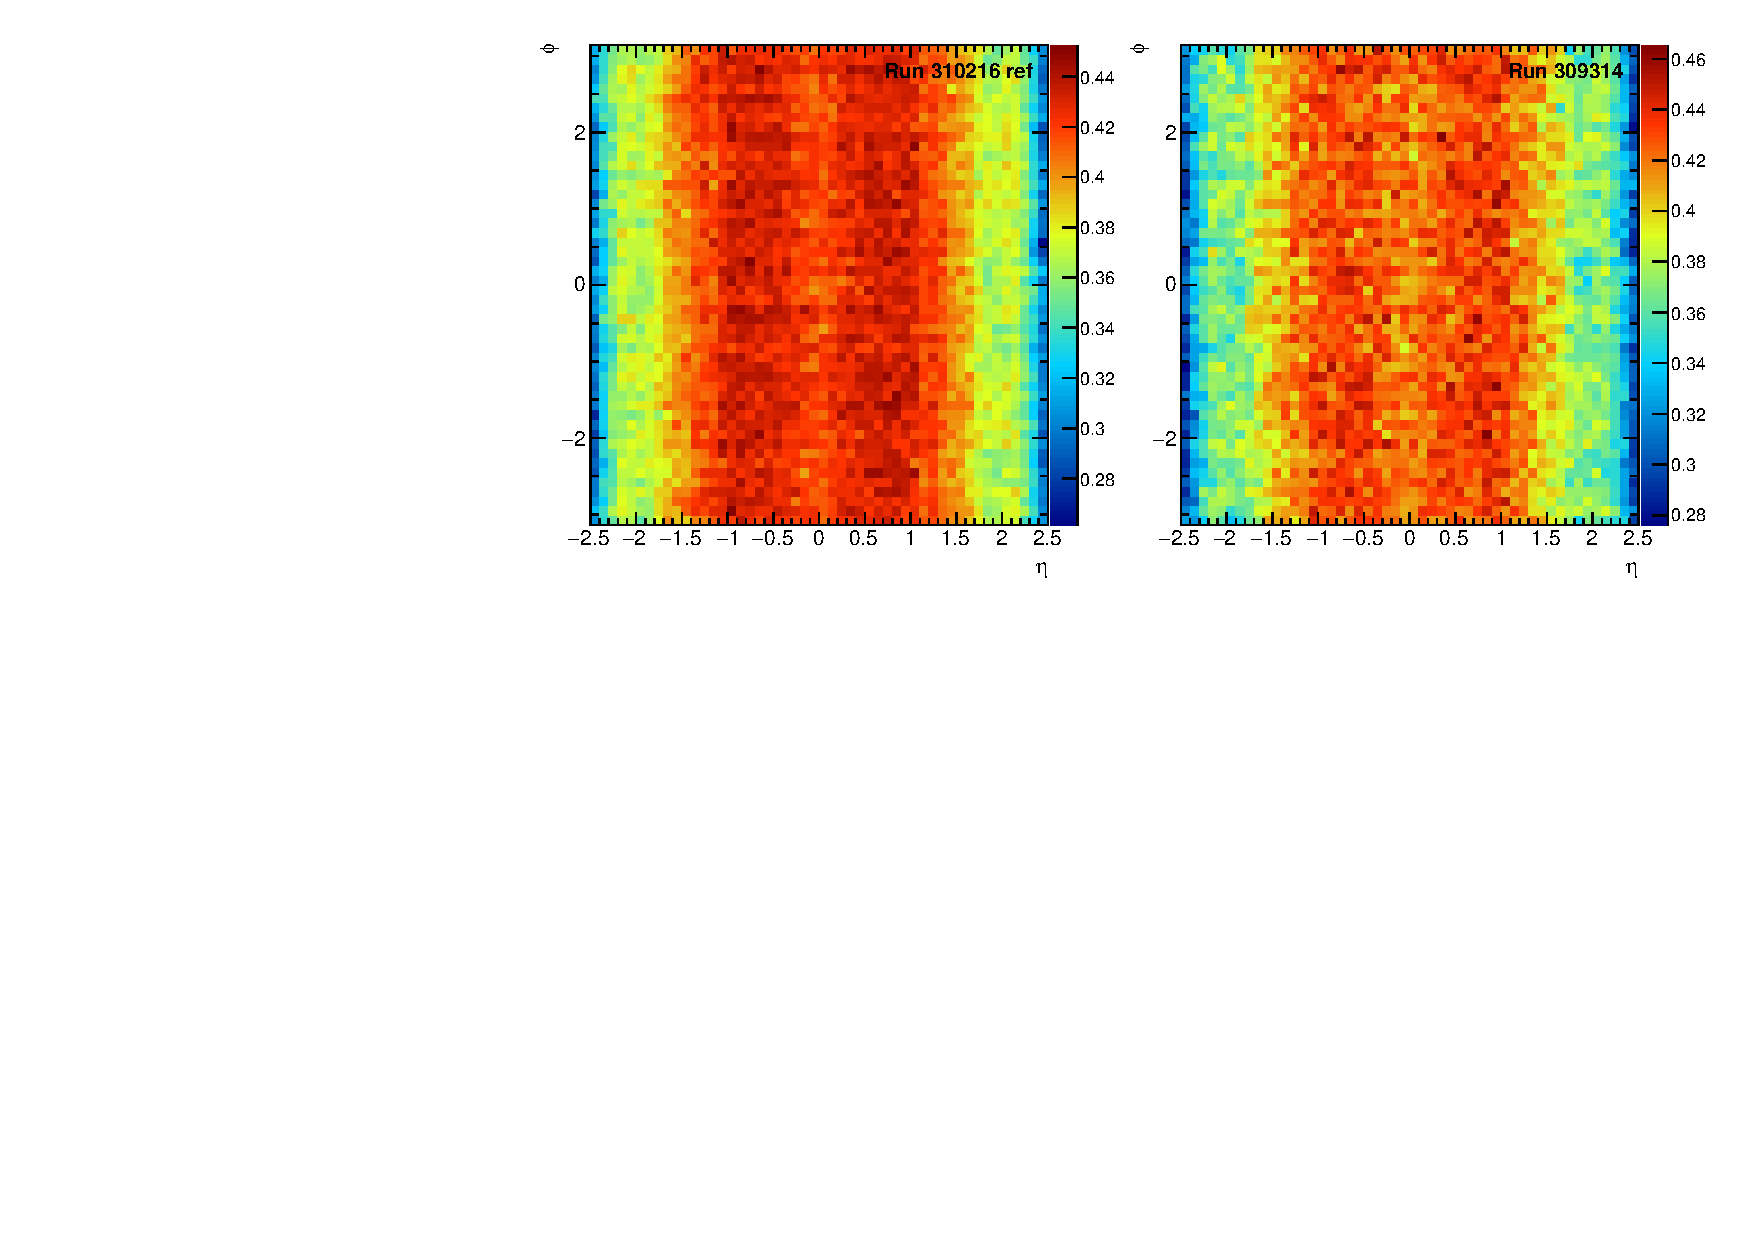
\includegraphics[width=0.9\linewidth]{figs/sec_evtSlc/GRLpp2016/309314_crr_eta_phi.pdf}
\caption{2D map of raw $\eta$-$\phi$ distribution: a comparison between run 309314 and run 310216.}
\label{fig:GRLpp2016_309314_eta_phi}
\end{figure}
Finally, fig.~\ref{fig:GRLpp2016_309314_eta_phi} shows the 2D map of raw $\eta$-$\phi$ distribution. "raw" means the tracks are not weighted by tracking efficiency. The distributions are very consistent.

As a conclusion, even though beam spot is not constraint in these two runs, various tracking quantities are very consistent with the reference run. Due to these reasons, we will include these two runs into the $pp$ analysis.




\subsection{$pp$ 5.02 TeV}
In 2015 before the Pb+Pb run, low-$\mu$ and intermediate-$\mu$ 5.02 TeV $pp$ data was collected with ATLAS detectors. Since this reference run is right after previous $pp$ runs, the track selection is identical to 13 TeV $pp$. All the runs, with GRL selection, are included in this analysis and they are listed as below:
\begin{itemize}

\item Run 286282, peak $\mu=0.58$, 37.3 million events from MinBias stream
\begin{itemize}[leftmargin=*]
\item[] \verb|data15_5TeV.00286282.physics_MinBias.recon.AOD.r7744/|
\end{itemize}

\item Run 286328, peak $\mu=1.58$, 5.8 million events from MinBias stream
\begin{itemize}[leftmargin=*]
\item[] \verb|data15_5TeV.00286328.physics_MinBias.recon.AOD.r7744/|
\end{itemize}

\item Run 286361, peak $\mu=1.34$, 3.5 million events from MinBias stream
\begin{itemize}[leftmargin=*]
\item[] \verb|data15_5TeV.00286361.physics_MinBias.recon.AOD.r7744/|
\end{itemize}

\item Run 286364, peak $\mu=1.58$, 7.9 million events from MinBias stream
\begin{itemize}[leftmargin=*]
\item[] \verb|data15_5TeV.00286364.physics_MinBias.recon.AOD.r7744/|
\end{itemize}

\item Run 286367, peak $\mu=0.67$, 1.7 million events from MinBias stream
\begin{itemize}[leftmargin=*]
\item[] \verb|data15_5TeV.00286367.physics_MinBias.recon.AOD.r7744/|
\end{itemize}

\item Run 286411, peak $\mu=1.33$, 10.8 million events from MinBias stream
\begin{itemize}[leftmargin=*]
\item[] \verb|data15_5TeV.00286411.physics_MinBias.recon.AOD.r7744/|
\end{itemize}

\item Run 286474, peak $\mu=1.25$, 5.3 million events from MinBias stream
\begin{itemize}[leftmargin=*]
\item[] \verb|data15_5TeV.00286474.physics_MinBias.recon.AOD.r7744/|
\end{itemize}

\end{itemize}

Similar as 13 TeV $pp$, the triggers applied in 5 TeV $pp$ have two components: MinBias and HMT. A list of all the major MinBias and HMT triggers used in this analysis is summarized as follows:
\begin{itemize}
\item \verb|HLT_mb_sptrk|
\item \verb|HLT_noalg_mb_L1MBTS_1|
\item \verb|HLT_mb_sp800_pusup400_trk50_hmt_L1TE5|
\item \verb|HLT_mb_sp900_pusup500_trk60_hmt_L1TE5|
\item \verb|HLT_mb_sp1200_pusup700_trk70_hmt_L1TE5|
\item \verb|HLT_mb_sp1400_pusup550_trk90_hmt_L1TE10|
\end{itemize}
where a new trigger item has been introduced:
\begin{itemize}
\item \verb|pusup|: maximum number of hits from a vertex, used to suppress pile-up events before track reconstruction;
\end{itemize}

\begin{figure}[H]
\centering
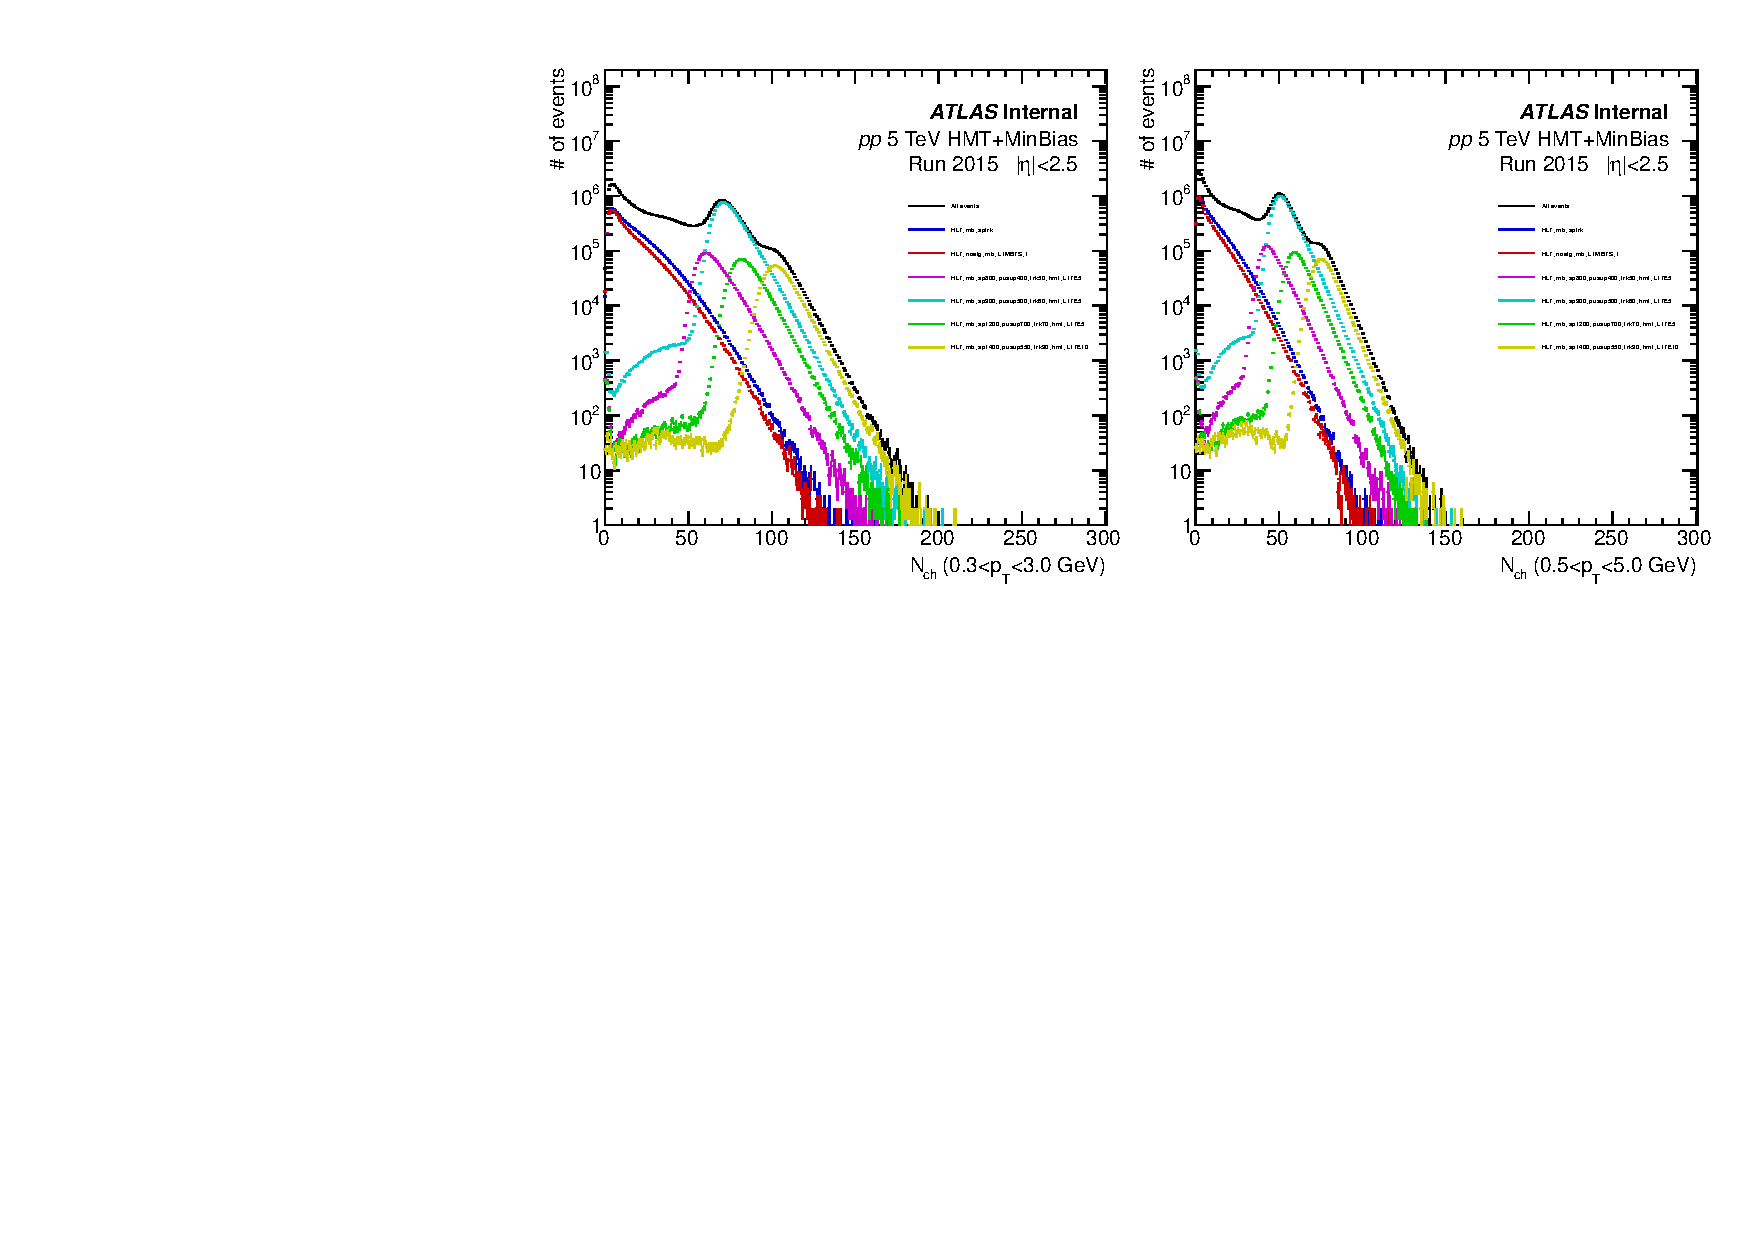
\includegraphics[width=.9\linewidth]{figs/sec_evtSlc/trkDis_pp5.pdf}
\caption{Distribution of number of tracks with two $p_{T}$ thresholds: $0.3<p_{T}<3.0$ GeV and $0.5<p_{T}<5.0$ GeV, in 13 TeV $pp$ run period 4. The major MinBias and HMT triggers are plotted separately.}
\label{fig:trkDis_pp5}
\end{figure}
The summary of statistics with all the major triggers used in this analysis are shown in Fig.~\ref{fig:trkDis_pp5}.

\begin{figure}[H]
\centering
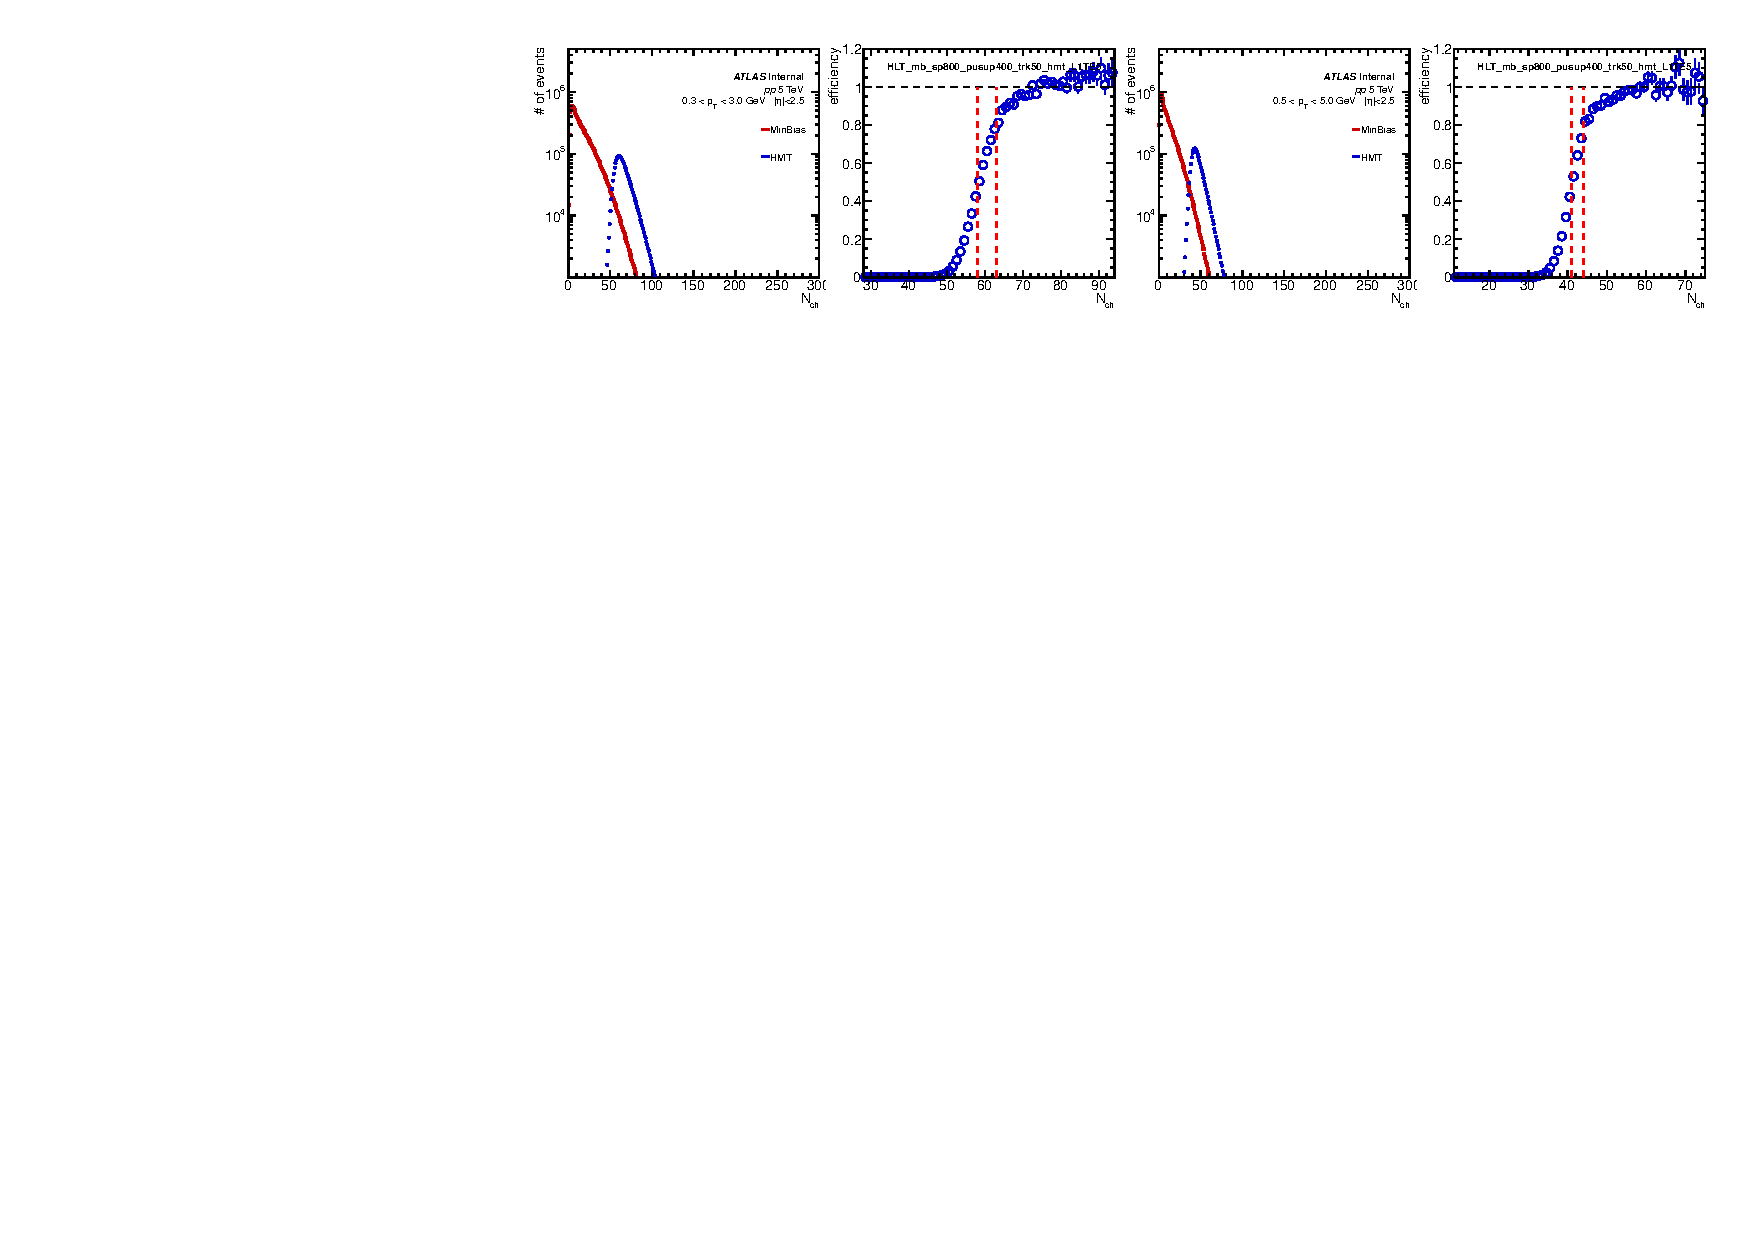
\includegraphics[width=1.\linewidth]{figs/sec_evtSlc/trigEff_pp5/trigEff_Trig18.pdf}
\end{figure}
\begin{figure}[H]
\centering
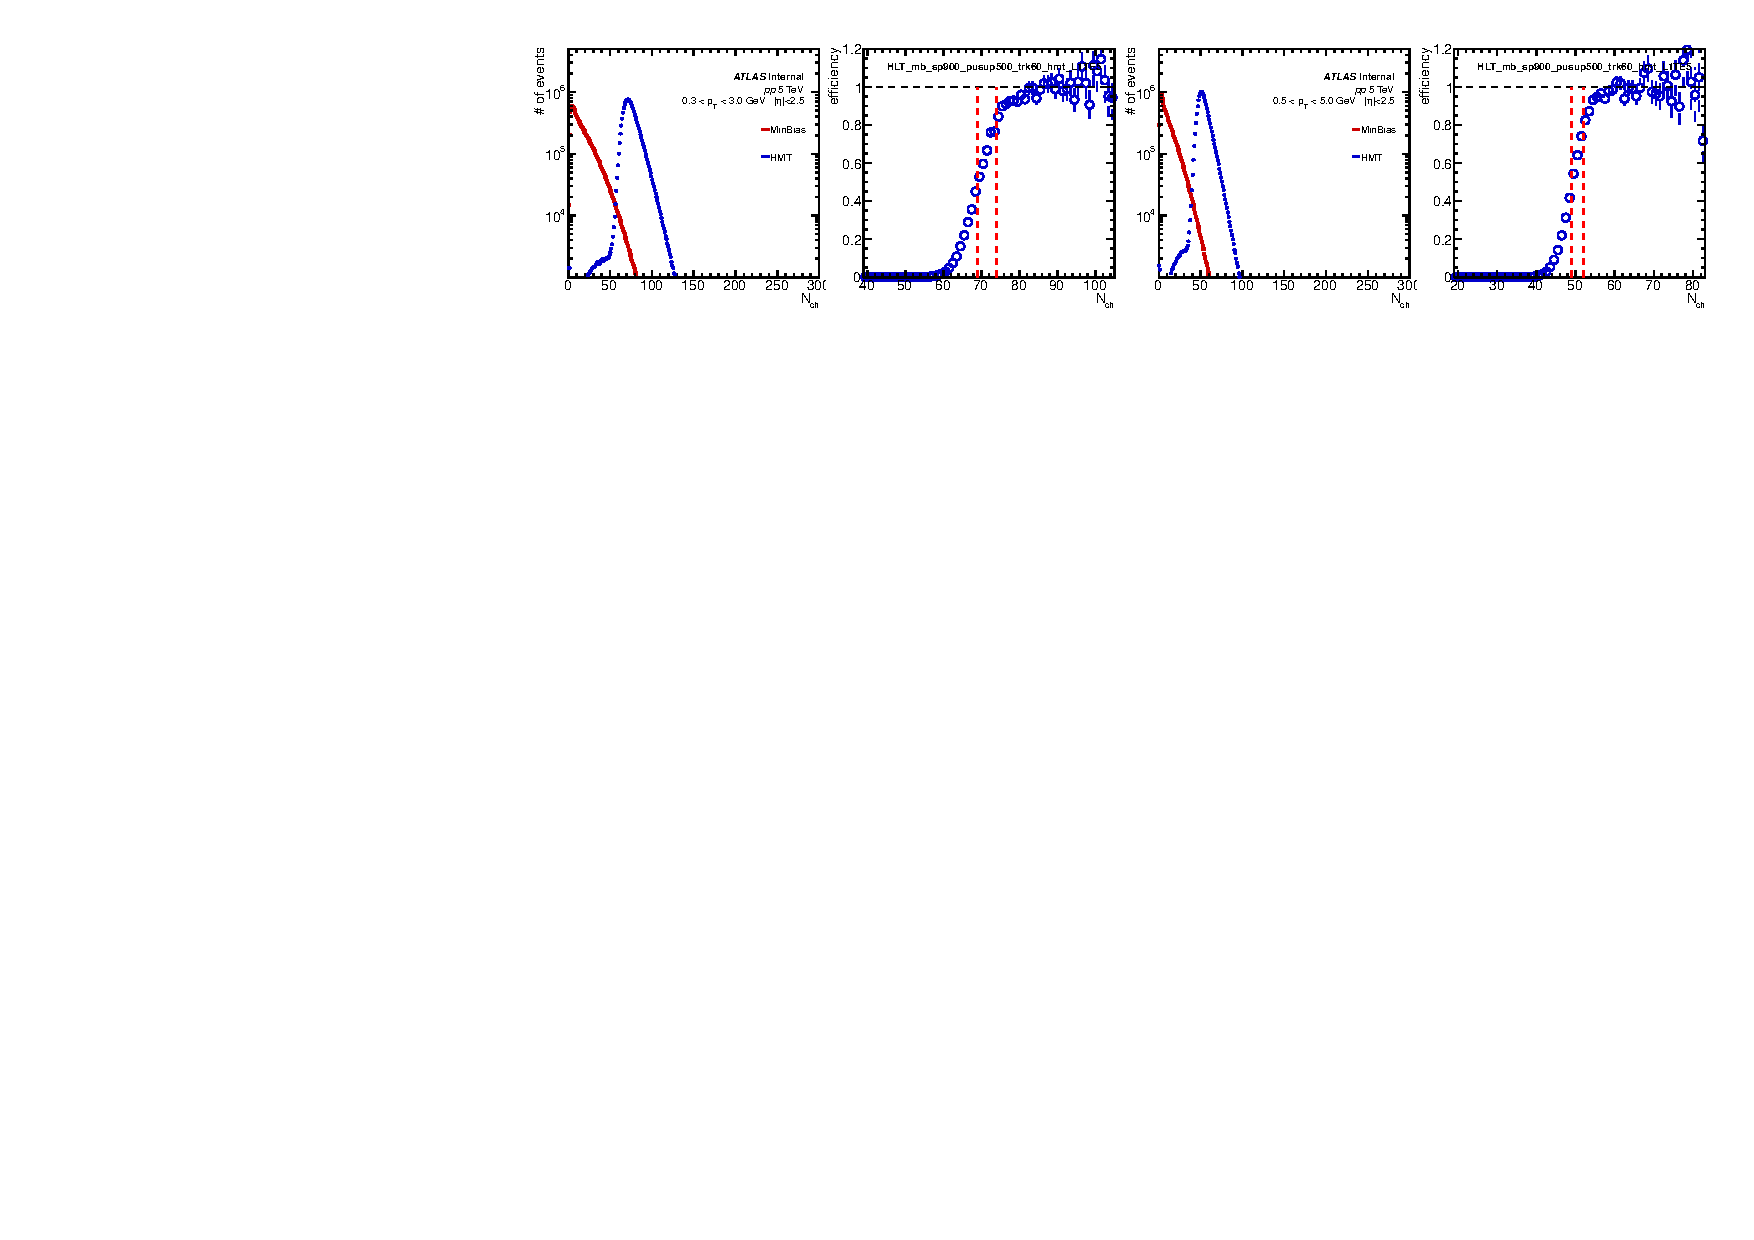
\includegraphics[width=1.\linewidth]{figs/sec_evtSlc/trigEff_pp5/trigEff_Trig19.pdf}
\end{figure}
\begin{figure}[H]
\centering
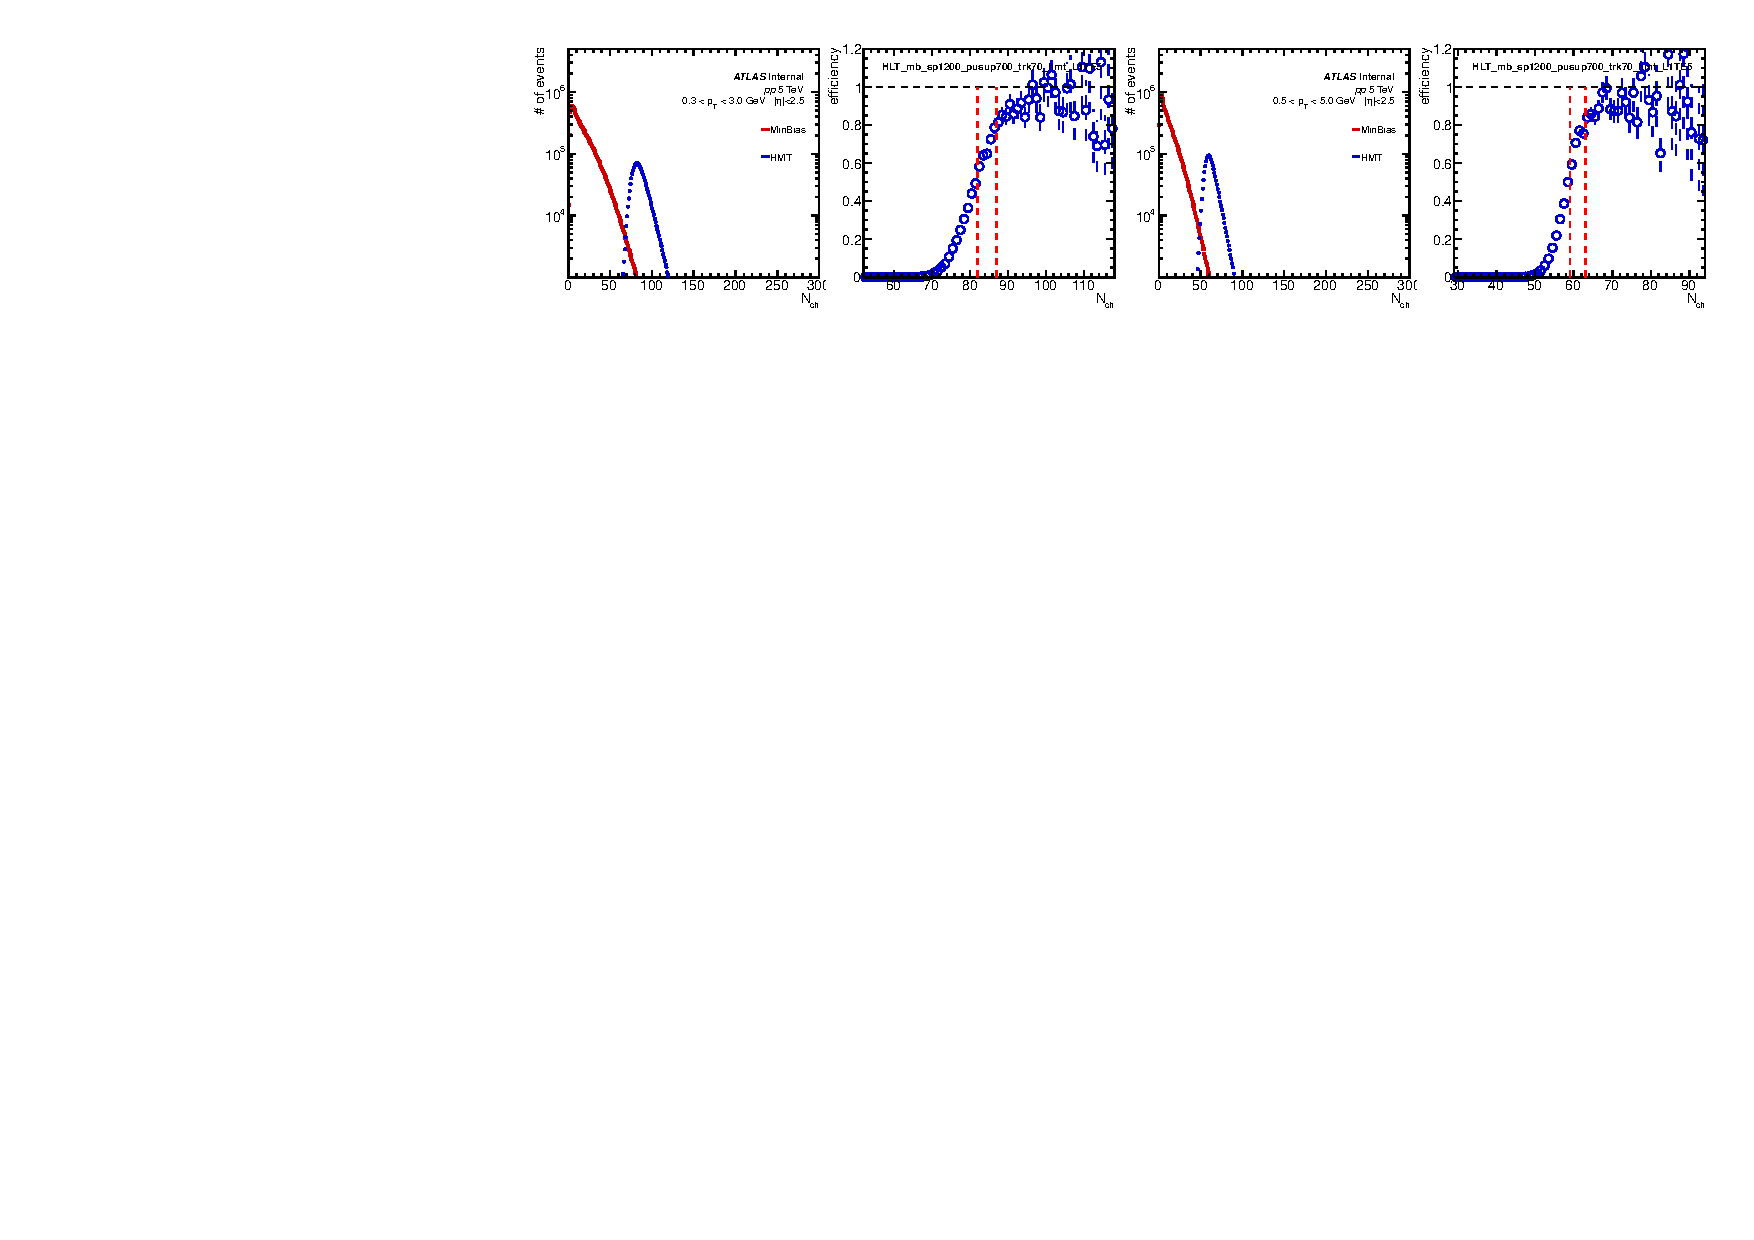
\includegraphics[width=1.\linewidth]{figs/sec_evtSlc/trigEff_pp5/trigEff_Trig20.pdf}
\end{figure}
\begin{figure}[H]
\centering
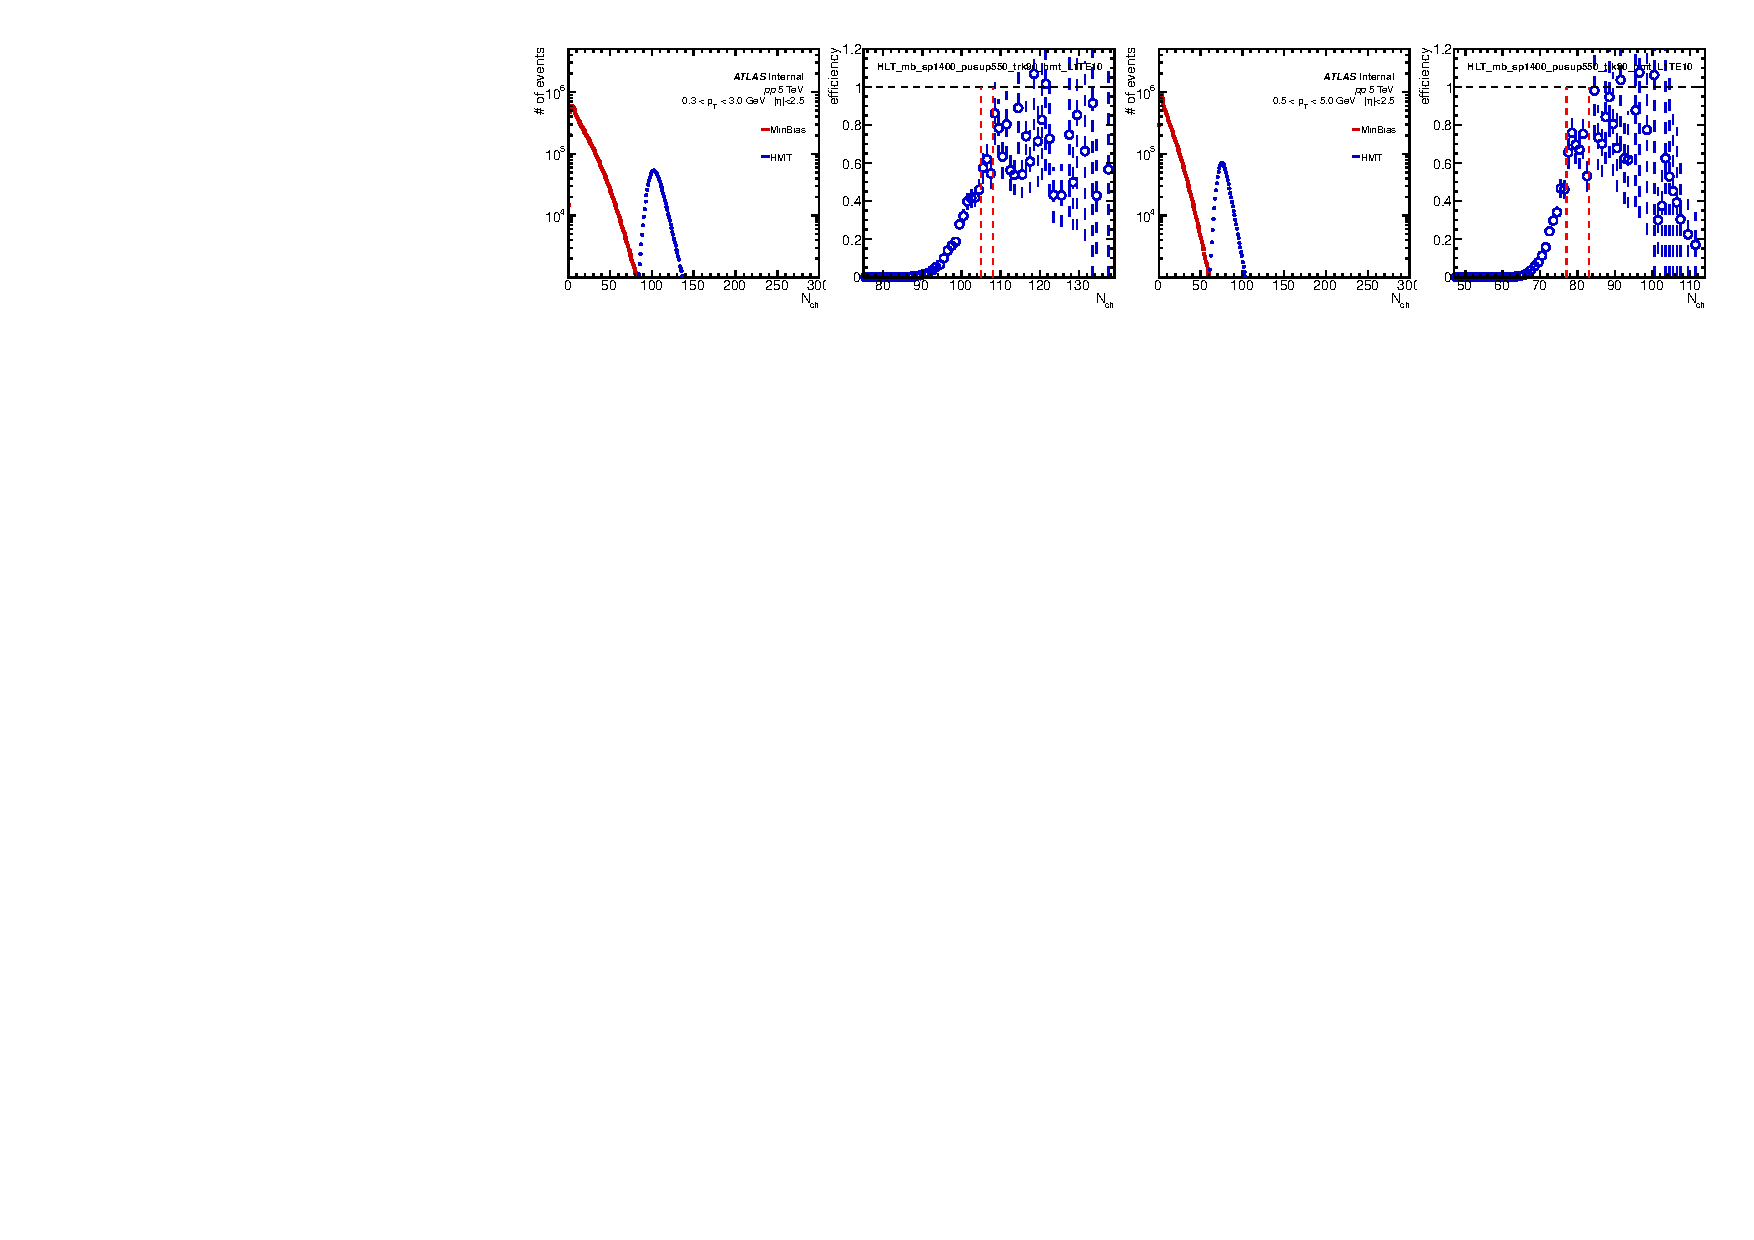
\includegraphics[width=1.\linewidth]{figs/sec_evtSlc/trigEff_pp5/trigEff_Trig21.pdf}
\caption{Trigger efficiencies of all major HMT triggers as a function of number of tracks in two $p_{T}$ ranges: $0.3<p_{T}<3.0$ GeV and $0.5<p_{T}<5.0$ GeV, from 5 TeV $pp$ run. Efficiency is calculated relative to the corresponding MinBias trigger in this run period then scaled to 1.0 in the large $N_{ch}$ region. The two red dash lines indicate 50$\%$ and 80$\%$ efficiency cuts.}
\label{fig:trigEff_pp5}
\end{figure}
Trigger efficiencies of all the major HMT triggers are summarized in Fig.~\ref{fig:trigEff_pp5}, where efficiencies are shown for two $p_{T}$ ranges separately: $0.3<p_{T}<3.0$ GeV and $0.5<p_{T}<5.0$ GeV.

\subsubsection{PYTHIA for $pp$ 5.02 TeV data}
Since the 5 TeV $pp$ run is close to 13 TeV run in time, the detector effects between the two runs should be similar. For his reason, tracking efficiency and fraction of fake tracks extracted from 13 TeV PYTHIA is applied to 5 TeV $pp$ data.

\subsubsection{Impact of ID misalignment}
In order to study the effect of ID misalignment, the package \verb|InDetTrackSystema9csTools-00-00-18| was used. The 5 TeV $pp$ cumulant are recalculated with the corrected track momenta and compared to the default measurement.

\begin{figure}
\centering
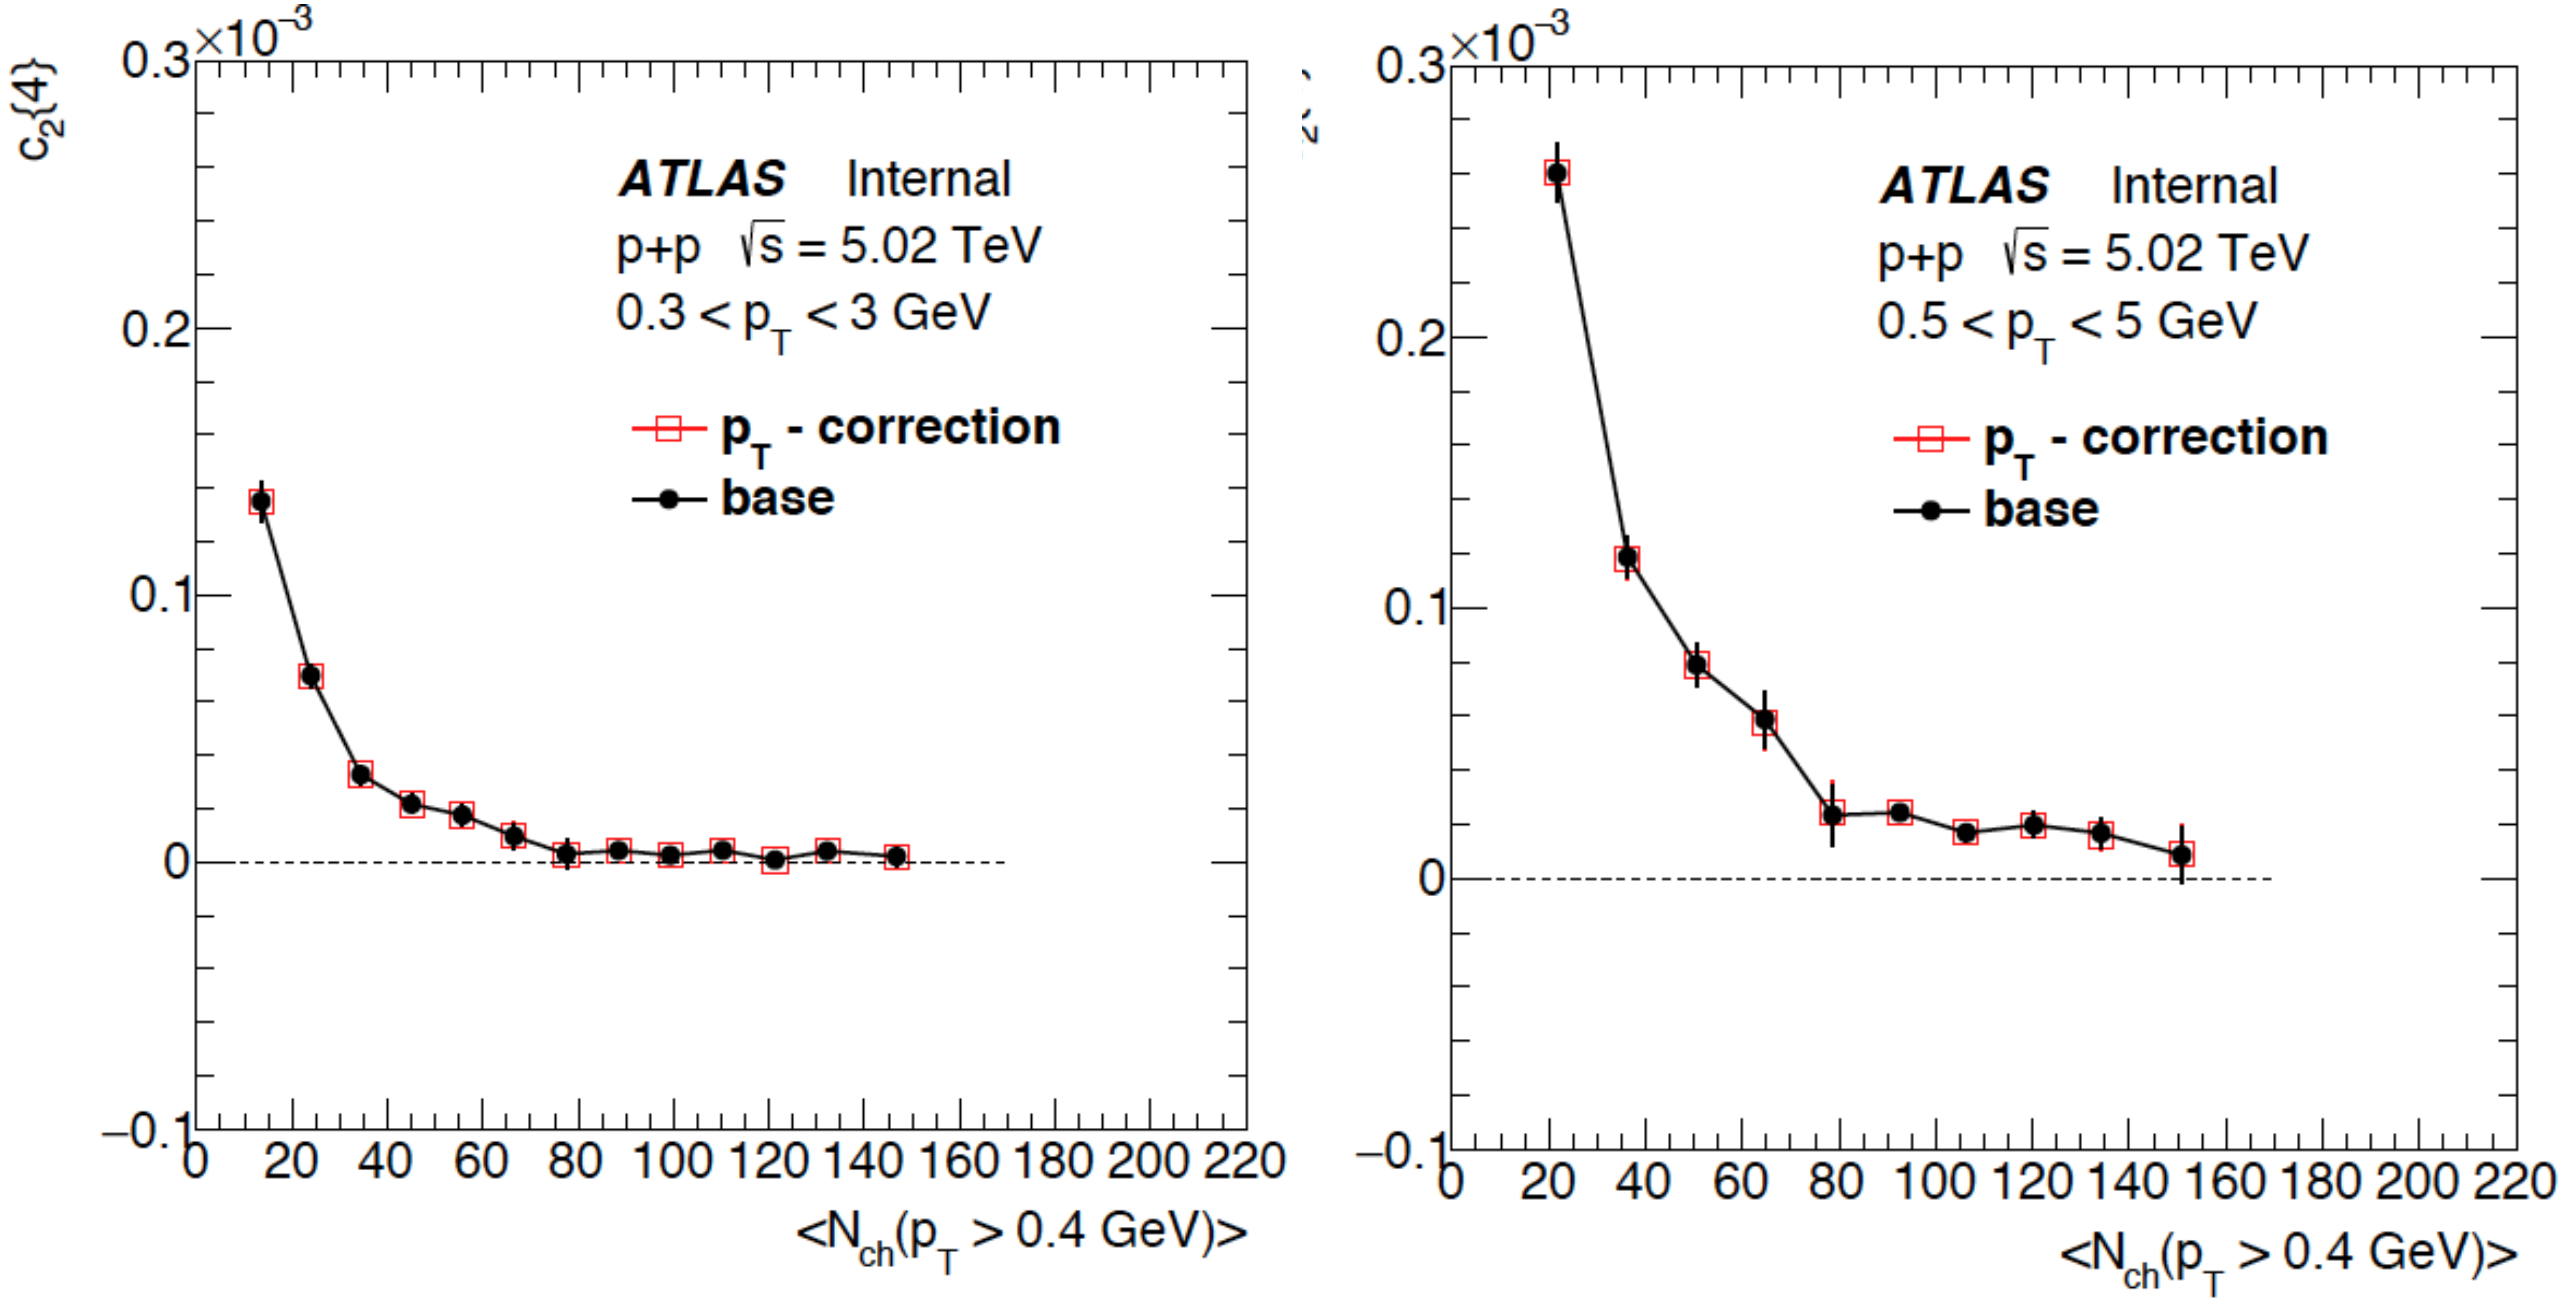
\includegraphics[width=1.\linewidth]{figs/sec_evtSlc/ID_alignment_pp5.png}
\caption{$c_{2}{4}$ measured with default and $p_{\text{T}}$ corrected, for $0.3<p_{\text{T}}<3.0$ GeV (left) and $0.5<p_{\text{T}}<5.0$ GeV (right).}
\label{fig:ID_alignment_pp5}
\end{figure}
For $c_{2}{4}$ the effects of ID misalignment for low multiplicity (up to 60) is at $0.1\%$ level. At higher multiplicity the difference is smaller than statistical errors. This concludes that the ID misalignment has minimal impact on this analysis.

\subsection{$p$+Pb 5.02 TeV}
5.02 TeV $p$+Pb data have been collected in 2013~\cite{Aad:2012bu} and 2016. Since the event and tracking selections are quite different between Run 1 and Run 2, they will be discussed separately in the following sections.

\subsubsection{2013 $p$+Pb}
In 2013, low-$\mu$ 5.02 TeV $p$+Pb data was collected with ATLAS detectors. In additional to GRL selection, each event also needs to pass the MBTS cuts:
\begin{itemize}
\item $|\text{time}_{A}|$ or $|\text{time}_{C}|$ must not equal 75 or 0 ns;
\item $|\text{time}_{A}-\text{time}_{C}|<10$ ns;
\end{itemize}
and the pile-up events are suppressed by rejecting events containing more than one good reconstructed vertex. The remaining pileup events are further suppressed based on the signal in the ZDC on the Pb-fragmentation side. This signal is calibrated to the number of detected neutrons ($N_{n}$) based on the location of the peak corresponding to a single neutron. The distribution of $N_{n}$ in events with pileup is broader than that for the events without pileup. Hence, a simple cut on the high tail end of the ZDC signal distribution further suppresses the pileup, while retaining more than 98$\%$ of the events without pileup. After this pileup rejection procedure, the residual pileup fraction is estimated to be 1$\%$ in the event class with the highest track multiplicity studied in this analysis. For details of this pile-up rejection, refer to the internal note of flow measurements in $p$+Pb~\cite{atlas:9}.

The track selection criteria is $p$+Pb is slightly different from $pp$~\cite{Aad:2015gqa, Aad:2016mok}:
\begin{itemize}
\item Tracks are from primary vertex
\item Present hit in B-Layer if expected
\item At least 1 pixel hit
\item $p_{T}<300$ MeV: at least 4 SCT hits + dead sensors
\item $p_{T}>300$ MeV: at least 6 SCT hits + dead sensors
\item significance of $d_{0}$ is $<3.0$
\item significance of $z_{0}\text{sin}\theta$ is $<3.0$
\item $|\eta|\le 2.5$
\item $p_{T}\ge 200$ MeV
\end{itemize}
In additional, an additional tighter cut defined to be the track selection requirements in Pb-Pb analysis is used to check the stability of results in the systematics section.

All the runs included in this analysis are listed as follows. A special reprocessing was done for these runs so that the lowest $p_{T}$ goes down to 0.1 GeV.

\begin{itemize}

\item Run 217999, 4.7 million events from MinBias stream
\begin{itemize}[leftmargin=*]
\item[] \verb|data13_hip.00217999.physics_MinBias.merge.NTUP_HI.r5813_p1729/|
\end{itemize}

\item Run 218006, 2.7 million events from MinBias stream
\begin{itemize}[leftmargin=*]
\item[] \verb|data13_hip.00218006.physics_MinBias.merge.NTUP_HI.r5813_p1729/|
\end{itemize}

\item Run 218048, 6.6 million events from MinBias stream
\begin{itemize}[leftmargin=*]
\item[] \verb|data13_hip.00218048.physics_MinBias.merge.NTUP_HI.r5813_p1729/|
\end{itemize}

\item Run 218118, 3.9 million events from MinBias stream
\begin{itemize}[leftmargin=*]
\item[] \verb|data13_hip.00218118.physics_MinBias.merge.NTUP_HI.r5813_p1729/|
\end{itemize}

\item Run 218168, 4.2 million events from MinBias stream
\begin{itemize}[leftmargin=*]
\item[] \verb|data13_hip.00218168.physics_MinBias.merge.NTUP_HI.r5813_p1729/|
\end{itemize}

\item Run 218179, 4.5 million events from MinBias stream
\begin{itemize}[leftmargin=*]
\item[] \verb|data13_hip.00218179.physics_MinBias.merge.NTUP_HI.r5813_p1729/|
\end{itemize}

\item Run 218213, 1.8 million events from MinBias stream
\begin{itemize}[leftmargin=*]
\item[] \verb|data13_hip.00218213.physics_MinBias.merge.NTUP_HI.r5813_p1729/|
\end{itemize}

\item Run 218222, 0.5 million events from MinBias stream
\begin{itemize}[leftmargin=*]
\item[] \verb|data13_hip.00218222.physics_MinBias.merge.NTUP_HI.r5813_p1729/|
\end{itemize}

\item Run 218301, 3.8 million events from MinBias stream
\begin{itemize}[leftmargin=*]
\item[] \verb|data13_hip.00218301.physics_MinBias.merge.NTUP_HI.r5813_p1729/|
\end{itemize}

\item Run 218338, 3.8 million events from MinBias stream
\begin{itemize}[leftmargin=*]
\item[] \verb|data13_hip.00218338.physics_MinBias.merge.NTUP_HI.r5813_p1729/|
\end{itemize}

\item Run 218391, 8.0 million events from MinBias stream
\begin{itemize}[leftmargin=*]
\item[] \verb|data13_hip.00218391.physics_MinBias.merge.NTUP_HI.r5813_p1729/|
\end{itemize}

\item Run 218436, 5.1 million events from MinBias stream
\begin{itemize}[leftmargin=*]
\item[] \verb|data13_hip.00218436.physics_MinBias.merge.NTUP_HI.r5813_p1729/|
\end{itemize}

\item Run 218473, 3.9 million events from MinBias stream
\begin{itemize}[leftmargin=*]
\item[] \verb|data13_hip.00218473.physics_MinBias.merge.NTUP_HI.r5813_p1729/|
\end{itemize}

\item Run 218589, 3.3 million events from MinBias stream
\begin{itemize}[leftmargin=*]
\item[] \verb|data13_hip.00218589.physics_MinBias.merge.NTUP_HI.r5813_p1729/|
\end{itemize}

\item Run 218677, 1.3 million events from MinBias stream
\begin{itemize}[leftmargin=*]
\item[] \verb|data13_hip.00218677.physics_MinBias.merge.NTUP_HI.r5813_p1729/|
\end{itemize}

\item Run 218679, 6.9 million events from MinBias stream
\begin{itemize}[leftmargin=*]
\item[] \verb|data13_hip.00218679.physics_MinBias.merge.NTUP_HI.r5813_p1729/|
\end{itemize}

\item Run 218716, 8.1 million events from MinBias stream
\begin{itemize}[leftmargin=*]
\item[] \verb|data13_hip.00218716.physics_MinBias.merge.NTUP_HI.r5813_p1729/|
\end{itemize}

\item Run 218751, 3.1 million events from MinBias stream
\begin{itemize}[leftmargin=*]
\item[] \verb|data13_hip.00218751.physics_MinBias.merge.NTUP_HI.r5813_p1729/|
\end{itemize}

\item Run 218771, 1.7 million events from MinBias stream
\begin{itemize}[leftmargin=*]
\item[] \verb|data13_hip.00218771.physics_MinBias.merge.NTUP_HI.r5813_p1729/|
\end{itemize}

\item Run 218783, 2.9 million events from MinBias stream
\begin{itemize}[leftmargin=*]
\item[] \verb|data13_hip.00218783.physics_MinBias.merge.NTUP_HI.r5813_p1729/|
\end{itemize}

\item Run 218829, 1.7 million events from MinBias stream
\begin{itemize}[leftmargin=*]
\item[] \verb|data13_hip.00218829.physics_MinBias.merge.NTUP_HI.r5813_p1729/|
\end{itemize}

\item Run 218898, 3.1 million events from MinBias stream
\begin{itemize}[leftmargin=*]
\item[] \verb|data13_hip.00218898.physics_MinBias.merge.NTUP_HI.r5813_p1729/|
\end{itemize}

\item Run 218940, 4.0 million events from MinBias stream
\begin{itemize}[leftmargin=*]
\item[] \verb|data13_hip.00218940.physics_MinBias.merge.NTUP_HI.r5813_p1729/|
\end{itemize}

\item Run 218968, 4.0 million events from MinBias stream
\begin{itemize}[leftmargin=*]
\item[] \verb|data13_hip.00218968.physics_MinBias.merge.NTUP_HI.r5813_p1729/|
\end{itemize}

\item Run 219001, 4.0 million events from MinBias stream
\begin{itemize}[leftmargin=*]
\item[] \verb|data13_hip.00219001.physics_MinBias.merge.NTUP_HI.r5813_p1729/|
\end{itemize}

\item Run 219028, 1.6 million events from MinBias stream
\begin{itemize}[leftmargin=*]
\item[] \verb|data13_hip.00219028.physics_MinBias.merge.NTUP_HI.r5813_p1729/|
\end{itemize}

\item Run 219055, 4.1 million events from MinBias stream
\begin{itemize}[leftmargin=*]
\item[] \verb|data13_hip.00219055.physics_MinBias.merge.NTUP_HI.r5813_p1729/|
\end{itemize}

\item Run 219089, 3.5 million events from MinBias stream
\begin{itemize}[leftmargin=*]
\item[] \verb|data13_hip.00219089.physics_MinBias.merge.NTUP_HI.r5813_p1729/|
\end{itemize}

\item Run 219111, 5.5 million events from MinBias stream
\begin{itemize}[leftmargin=*]
\item[] \verb|data13_hip.00219111.physics_MinBias.merge.NTUP_HI.r5813_p1729/|
\end{itemize}

\item Run 219114, 2.0 million events from MinBias stream
\begin{itemize}[leftmargin=*]
\item[] \verb|data13_hip.00219114.physics_MinBias.merge.NTUP_HI.r5813_p1729/|
\end{itemize}

\end{itemize}

Similar as $pp$, the triggers applied in 5 TeV $p$+Pb have two components: MinBias and HMT~\cite{Aad:2014lta, atlas:3}. A list of all the major MinBias and HMT triggers used in this analysis is summarized as follows:
\begin{itemize}
\item \verb|EF_mbMbts_1_1_counter|
\item \verb|EF_hip_trk100_TE10_counter|
\item \verb|EF_hip_trk130_TE10_counter|
\item \verb|EF_hip_trk150_TE50_counter|
\item \verb|EF_hip_trk185_TE50_counter|
\item \verb|EF_hip_trk200_TE65_counter|
\item \verb|EF_hip_trk225_TE65_counter|
\end{itemize}
where a new trigger item has been introduced:
\begin{itemize}
\item \verb|mbMbts_1_1|: HLT trigger requires at least 1 hit on both sides of MBTS;
\end{itemize}

\begin{figure}[H]
\centering
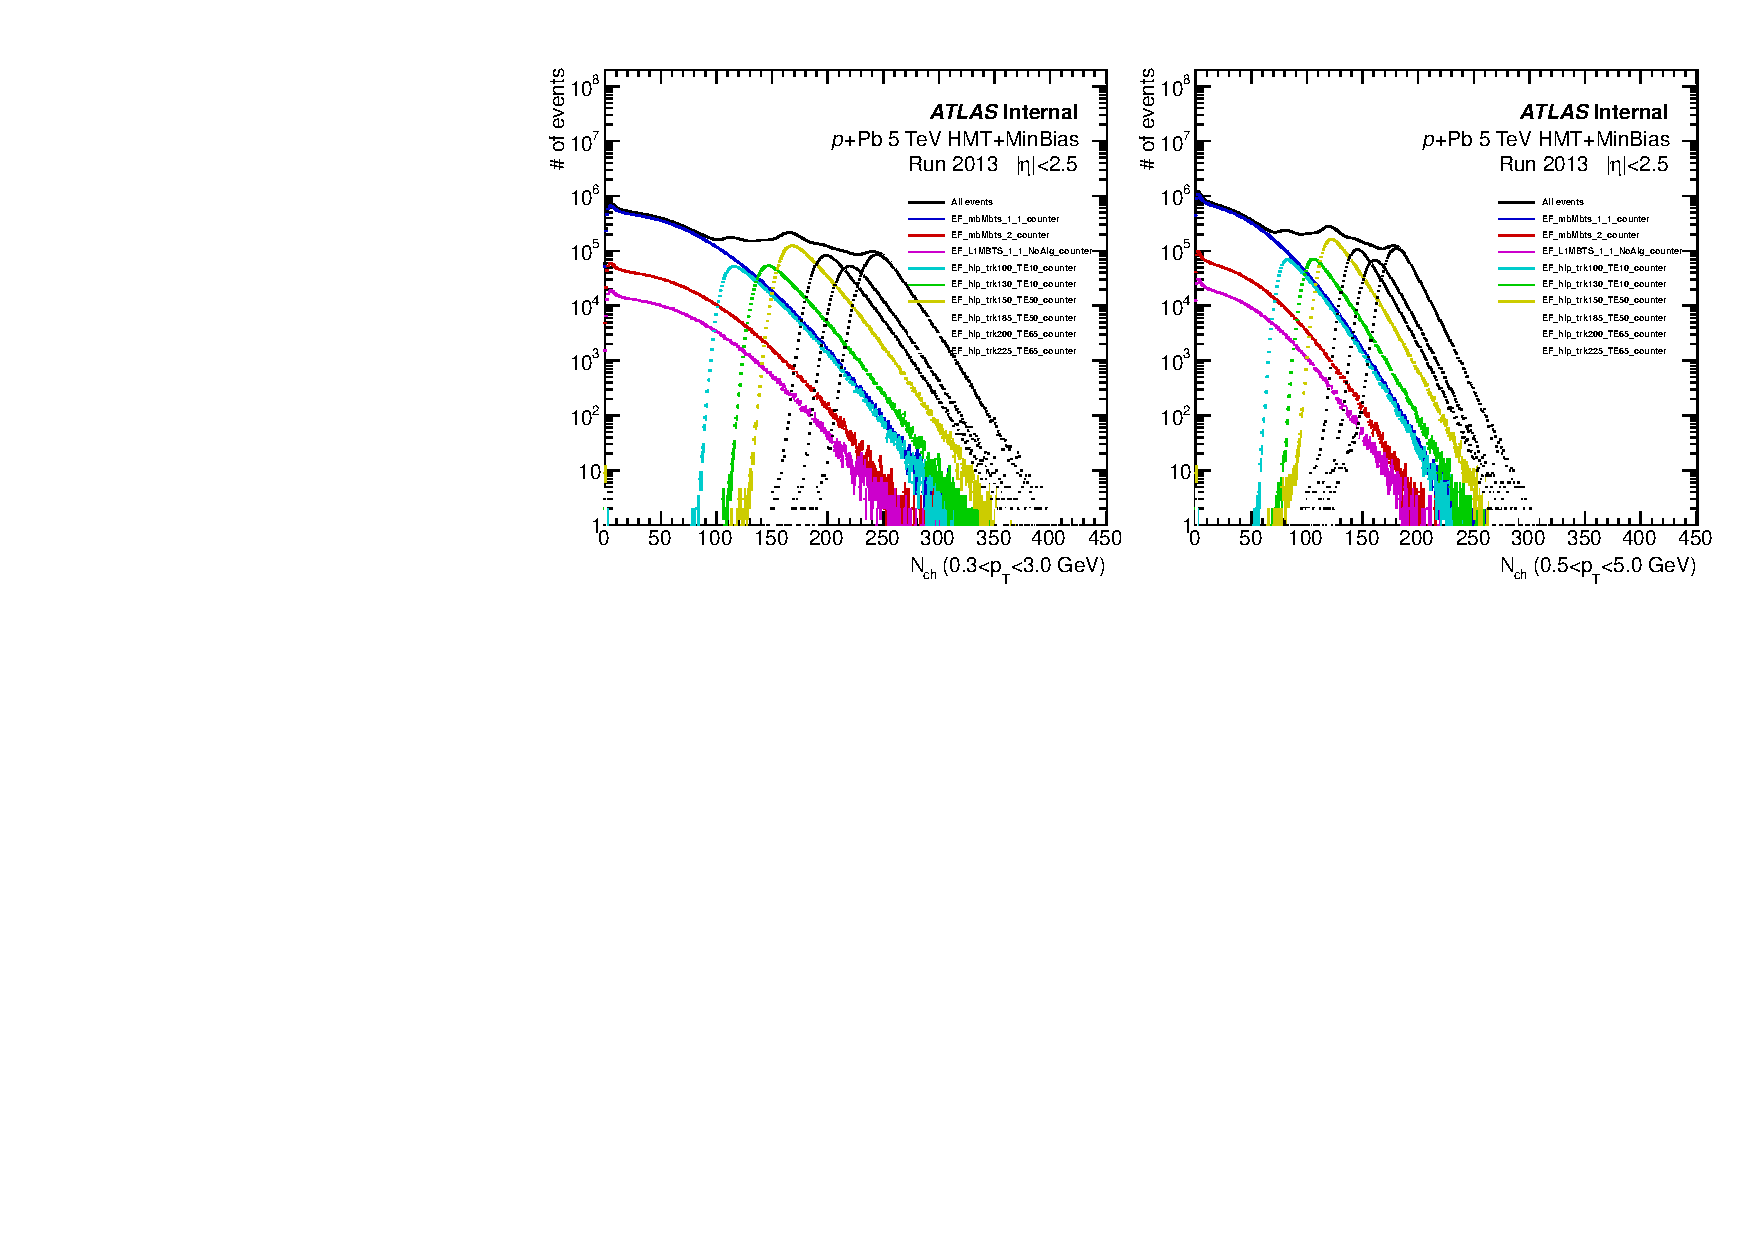
\includegraphics[width=.9\linewidth]{figs/sec_evtSlc/trkDis_pPb5_run1.pdf}
\caption{Distribution of number of tracks with two $p_{T}$ thresholds: $0.3<p_{T}<3.0$ GeV and $0.5<p_{T}<5.0$ GeV, in 5 TeV $p$+Pb run 2013. The major MinBias and HMT triggers are plotted separately.}
\label{fig:trkDis_pPb5_run1}
\end{figure}
The summary of statistics with all the major triggers used in this analysis are shown in Fig.~\ref{fig:trkDis_pPb5_run1}.

\begin{figure}[H]
\centering
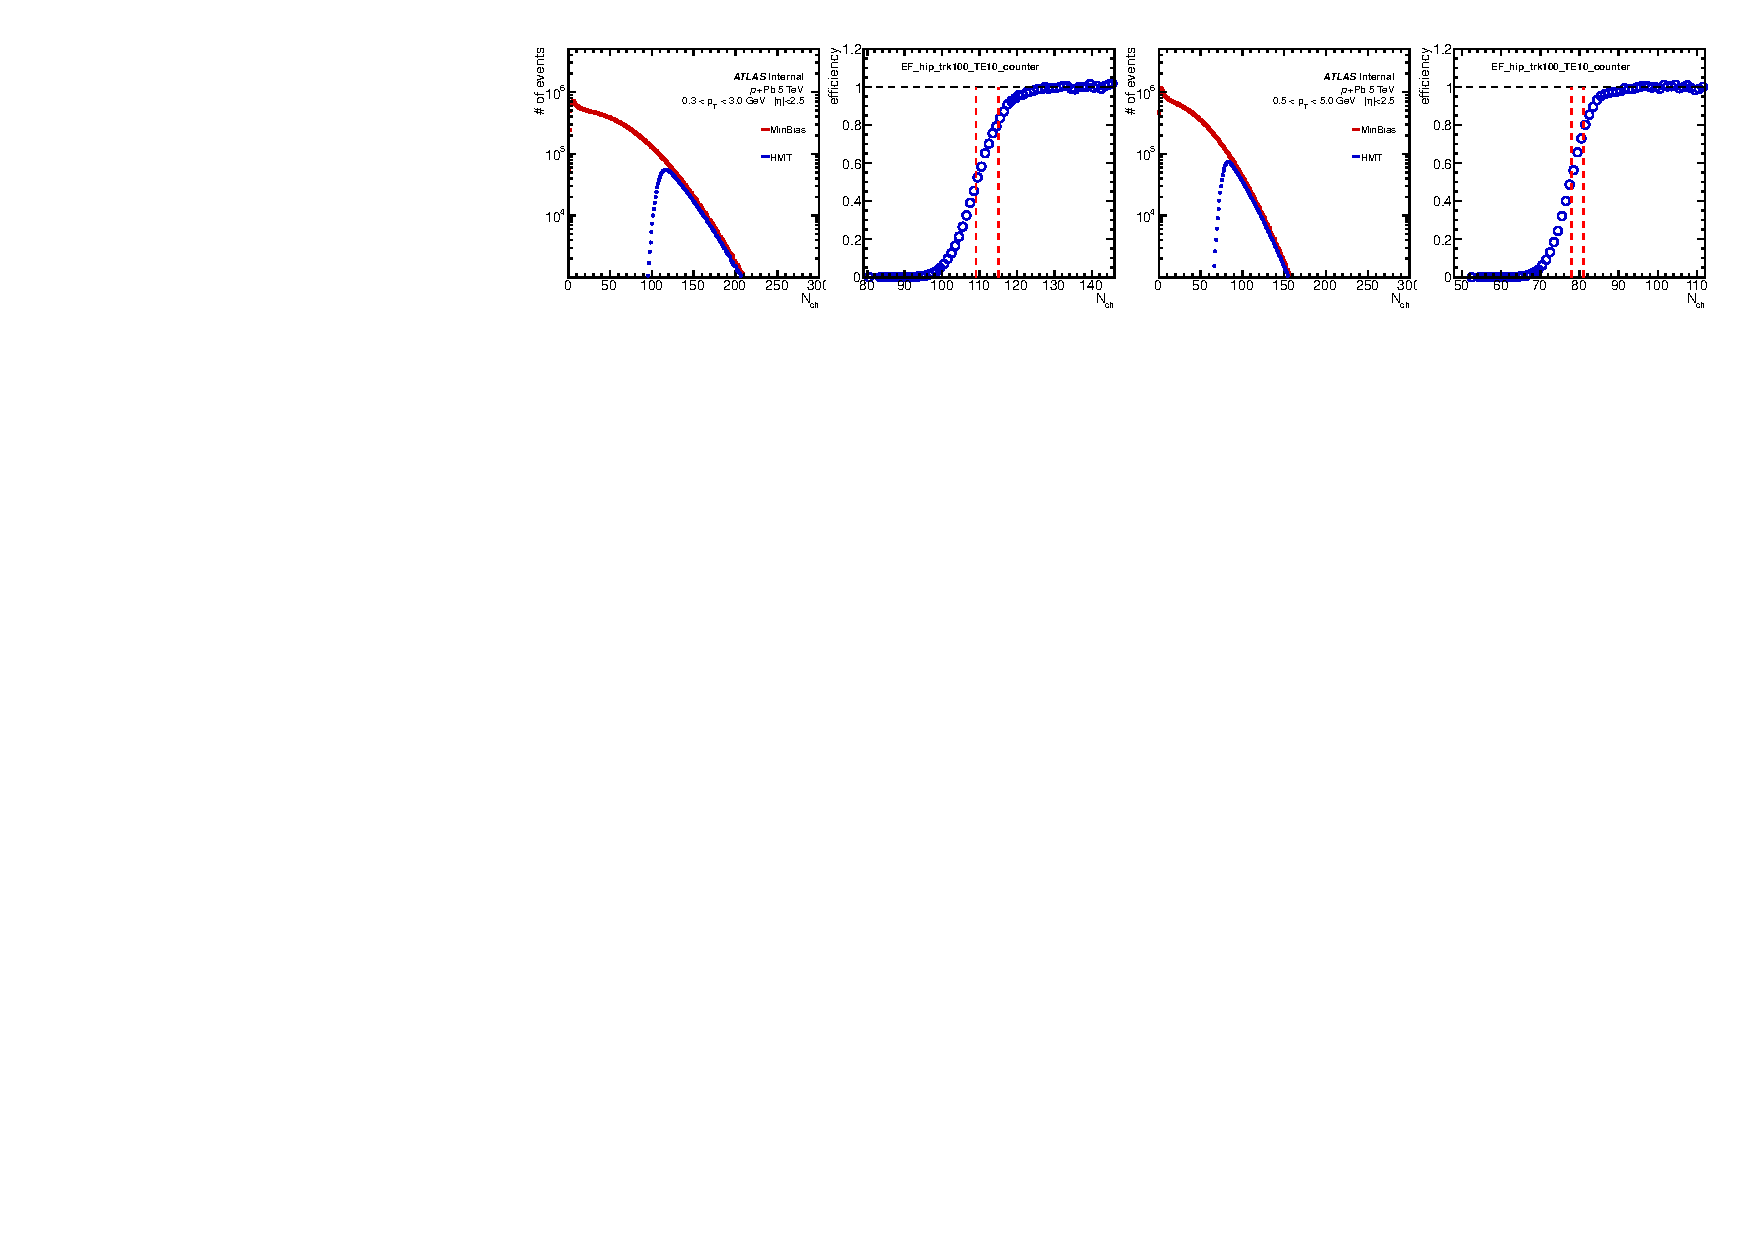
\includegraphics[width=1.\linewidth]{figs/sec_evtSlc/trigEff_pPb5_run1/trigEff_Trig8.pdf}
\end{figure}
\begin{figure}[H]
\centering
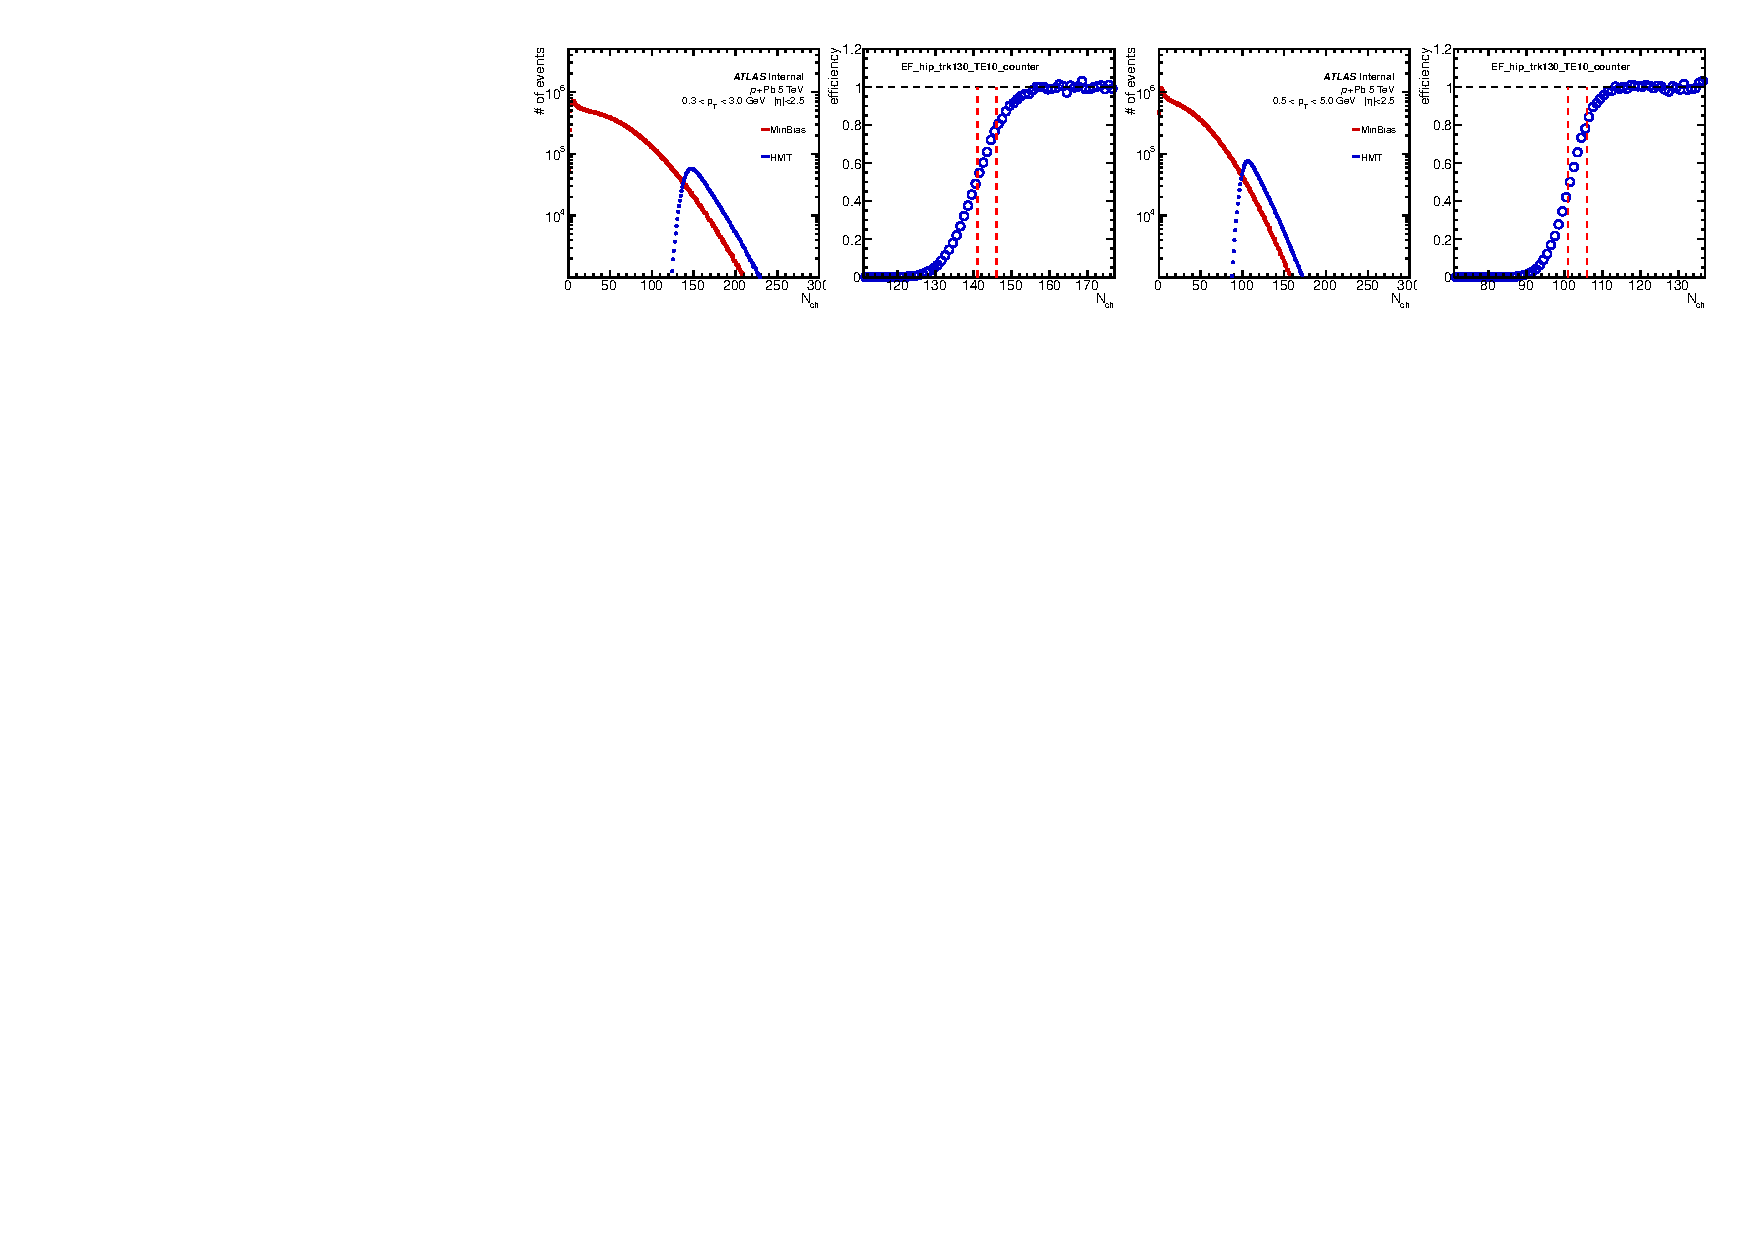
\includegraphics[width=1.\linewidth]{figs/sec_evtSlc/trigEff_pPb5_run1/trigEff_Trig9.pdf}
\end{figure}
\begin{figure}[H]
\centering
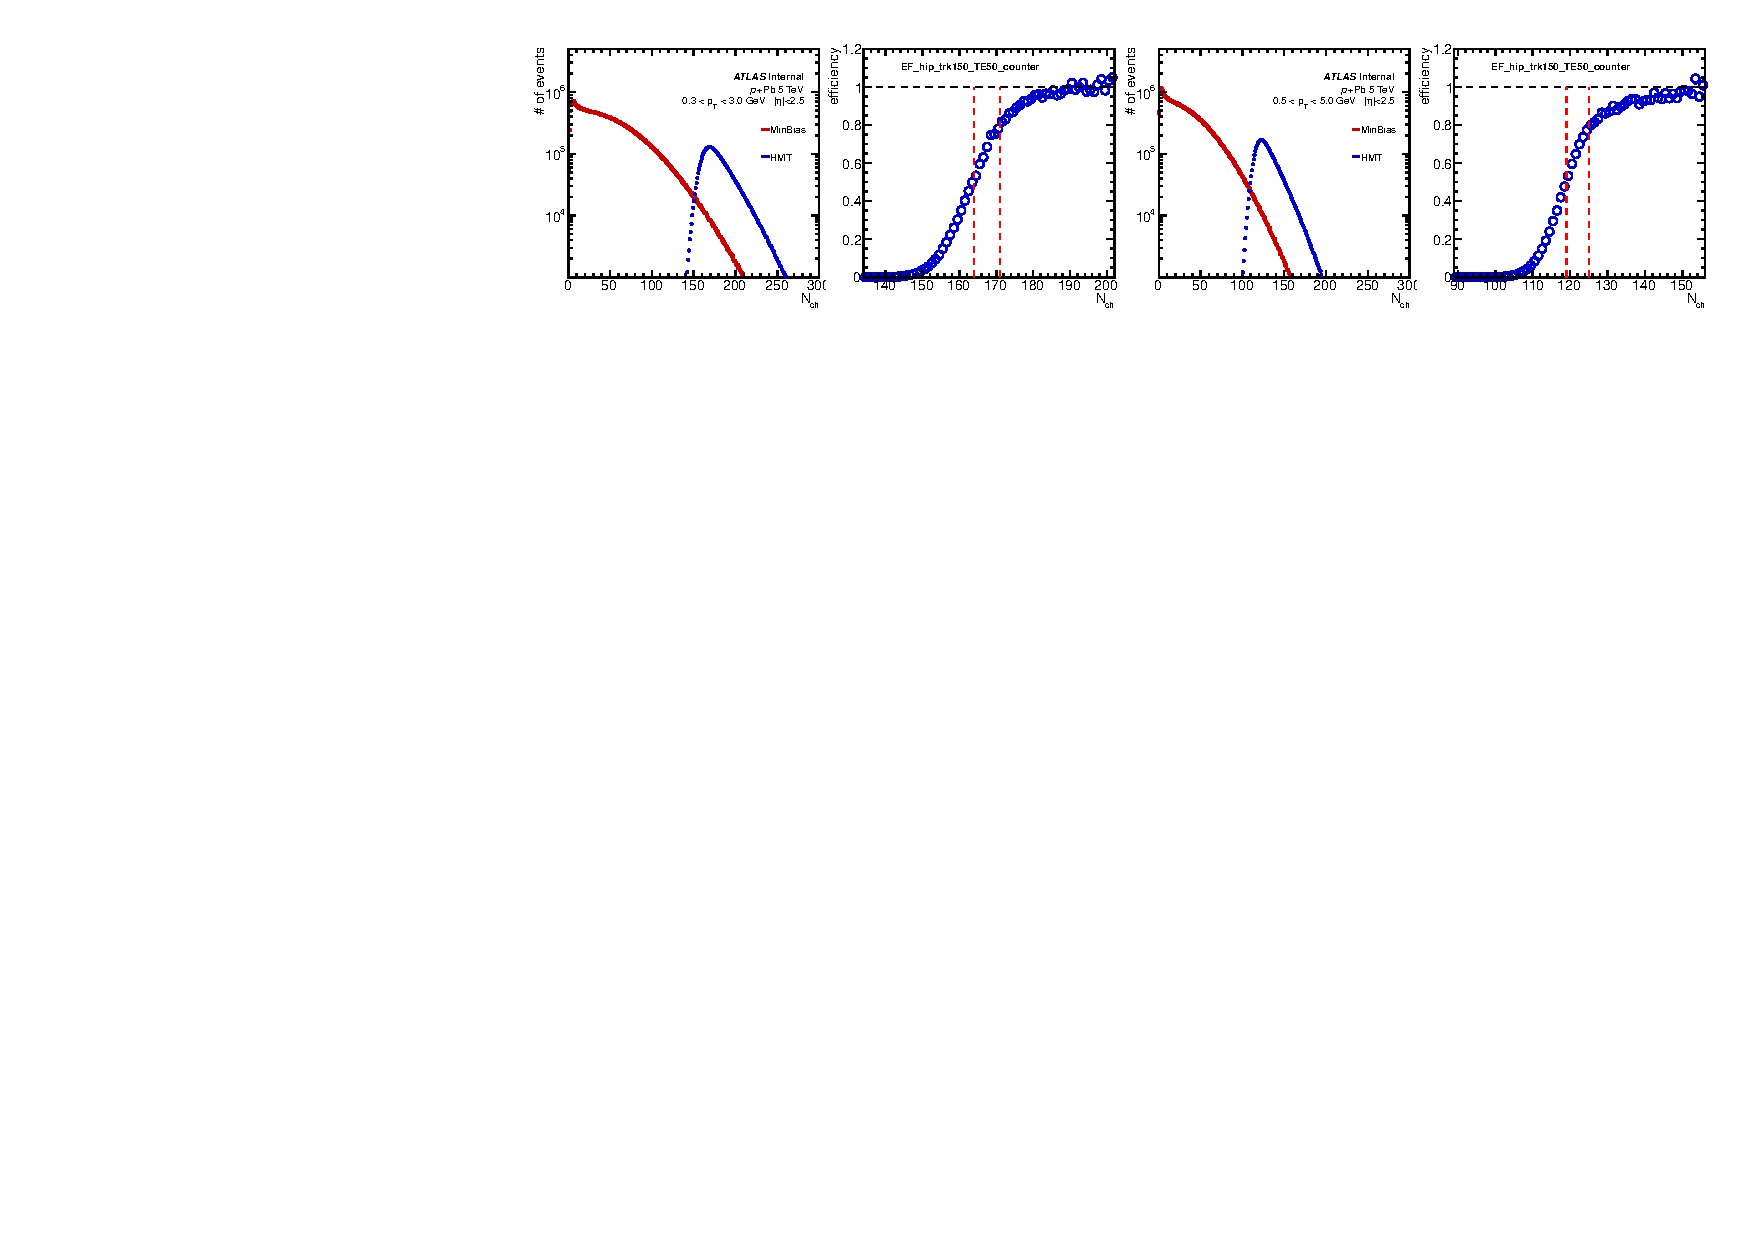
\includegraphics[width=1.\linewidth]{figs/sec_evtSlc/trigEff_pPb5_run1/trigEff_Trig10.pdf}
\end{figure}
\begin{figure}[H]
\centering
\includegraphics[width=1.\linewidth]{figs/sec_evtSlc/trigEff_pPb5_run1/trigEff_Trig11.pdf}
\end{figure}
\begin{figure}[H]
\centering
\includegraphics[width=1.\linewidth]{figs/sec_evtSlc/trigEff_pPb5_run1/trigEff_Trig12.pdf}
\end{figure}
\begin{figure}[H]
\centering
\includegraphics[width=1.\linewidth]{figs/sec_evtSlc/trigEff_pPb5_run1/trigEff_Trig13.pdf}
\caption{Trigger efficiencies of all major HMT triggers as a function of number of tracks in two $p_{T}$ ranges: $0.3<p_{T}<3.0$ GeV and $0.5<p_{T}<5.0$ GeV, from 5 TeV $p$+Pb run. Efficiency is calculated relative to the corresponding MinBias trigger in this run period then scaled to 1.0 in the large $N_{ch}$ region. The two red dash lines indicate 50$\%$ and 80$\%$ efficiency cuts.}
\label{fig:trigEff_pPb5_run1}
\end{figure}
Trigger efficiencies of all the major HMT triggers are summarized in Fig.~\ref{fig:trigEff_pPb5_run1}, where efficiencies are shown for two $p_{T}$ ranges separately: $0.3<p_{T}<3.0$ GeV and $0.5<p_{T}<5.0$ GeV.



\subsubsection{HIJING for 2013 $p$+Pb data}
Tracking efficiency and fraction of fake tracks have been extensively studied in previous $p$+Pb flow analyses~\cite{Aad:2014lta, atlas:3}. In this analysis we are re-using the efficiency map applied in the forward-backward multiplicity fluctuation paper \verb|ATL-COM-PHYS-2015-655|, where the tracking efficiency is estimated as a function of $\eta$, $p_{T}$, $N_{ch}$ and $z$ position of the vertex.



\subsubsection{2016 $p$+Pb}
In 2016, 5.02 TeV $p$+Pb data was collected with ATLAS detectors, with lower $\mu$ value than 2013. In additional to GRL selection, each event is required to have at least one vertex. Besides, problematic events are also removed:
\begin{itemize}
\item due to the liquid argon system
\item due to the tile calorimeter system
\item due to the SCT inner detector system
\item due to incomplete events (event information missing after TTC restarts)
\end{itemize}
and since the $\mu$ value of this year's run is much lower than 2013, cleaning pile-up events is not crucial. In the later section, with 2016 8.16 TeV $p$+Pb data, we will show that for events with $\mu<0.01$, pile-up effects are negligible.

Since this year's $p$+Pb run is right after the $pp$ run, the track selection criteria is identical to $pp$. An additional tighter $d_{0}$ and $z_{0}$ pointing cut is used to check the stability of results in the systematics section.

All the runs included in this analysis are listed as follows:
\begin{itemize}

\item Run 312649, 8.9 million events from MinBias stream
\begin{itemize}[leftmargin=*]
\item[] \verb|data16_hip5TeV.00312649.physics_Main.recon.AOD.f784_m1741|
\end{itemize}

\item Run 312796, 43 million events from MinBias stream
\begin{itemize}[leftmargin=*]
\item[] \verb|data16_hip5TeV.00312796.physics_Main.recon.AOD.f784_m1741|
\end{itemize}

\item Run 312837, 85 million events from MinBias stream
\begin{itemize}[leftmargin=*]
\item[] \verb|data16_hip5TeV.00312837.physics_Main.recon.AOD.f774_m1736|
\end{itemize}

\item Run 312937, 26 million events from MinBias stream
\begin{itemize}[leftmargin=*]
\item[] \verb|data16_hip5TeV.00312937.physics_Main.recon.AOD.f774_m1736|
\end{itemize}

\item Run 312945, 29 million events from MinBias stream
\begin{itemize}[leftmargin=*]
\item[] \verb|data16_hip5TeV.00312945.physics_Main.recon.AOD.f774_m1736|
\end{itemize}

\item Run 312968, 37 million events from MinBias stream
\begin{itemize}[leftmargin=*]
\item[] \verb|data16_hip5TeV.00312968.physics_Main.recon.AOD.f774_m1736|
\end{itemize}

\item Run 314199, 240 million events from MinBias stream
\begin{itemize}[leftmargin=*]
\item[] \verb|data16_hip5TeV.00314199.physics_Main.recon.AOD.f781_m1741|
\end{itemize}

\end{itemize}

Due to the reason that the intermediate $N_{ch}$ region is not covered by HMT triggers, several HMT triggers with intermediate $N_{ch}$ thresholds are specially designed before 2016 data taking. Together with MinBias triggers, all the major triggers used in this analysis is summarized as follows:
\begin{itemize}
\item \verb|HLT_noalg_mb_L1MBTS_1|
\item \verb|HLT_noalg_mb_L1MBTS_1_1|
\item \verb|HLT_mb_sp100_trk10_hmt_L1MBTS_1_1|
\item \verb|HLT_mb_sp100_trk20_hmt_L1MBTS_1_1|
\item \verb|HLT_mb_sp100_trk30_hmt_L1MBTS_1_1|
\item \verb|HLT_mb_sp100_trk60_hmt_L1MBTS_1_1|
\item \verb|HLT_mb_sp100_trk80_hmt_L1MBTS_1_1|
\item \verb|HLT_mb_sp100_trk100_hmt_L1MBTS_1_1|
\item \verb|HLT_mb_sp100_trk110_hmt_L1MBTS_1_1|
\end{itemize}
where all the HMT triggers are seeded on \verb|L1MBTS_1_1|, which is different from 2013 since the luminosity is much lower.

\begin{figure}[H]
\centering
\includegraphics[width=.9\linewidth]{figs/sec_evtSlc/trkDis_pPb5_run2.pdf}
\caption{Distribution of number of tracks with two $p_{T}$ thresholds: $0.3<p_{T}<3.0$ GeV and $0.5<p_{T}<5.0$ GeV, in 5 TeV $p$+Pb run 2016. The major MinBias and HMT triggers are plotted separately.}
\label{fig:trkDis_pPb5_run2}
\end{figure}
The summary of statistics with all the major triggers used in this analysis are shown in Fig.~\ref{fig:trkDis_pPb5_run2}.

\begin{figure}[H]
\centering
\includegraphics[width=1.\linewidth]{figs/sec_evtSlc/trigEff_pPb5_run2/trigEff_Trig6.pdf}
\end{figure}
\begin{figure}[H]
\centering
\includegraphics[width=1.\linewidth]{figs/sec_evtSlc/trigEff_pPb5_run2/trigEff_Trig8.pdf}
\end{figure}
\begin{figure}[H]
\centering
\includegraphics[width=1.\linewidth]{figs/sec_evtSlc/trigEff_pPb5_run2/trigEff_Trig10.pdf}
\end{figure}
\begin{figure}[H]
\centering
\includegraphics[width=1.\linewidth]{figs/sec_evtSlc/trigEff_pPb5_run2/trigEff_Trig11.pdf}
\caption{Trigger efficiencies of all major HMT triggers as a function of number of tracks in two $p_{T}$ ranges: $0.3<p_{T}<3.0$ GeV and $0.5<p_{T}<5.0$ GeV, from 2016 5 TeV $p$+Pb run. Efficiency is calculated relative to the corresponding MinBias trigger in this run period then scaled to 1.0 in the large $N_{ch}$ region. The two red dash lines indicate 50$\%$ and 80$\%$ efficiency cuts.}
\label{fig:trigEff_pPb5_run2}
\end{figure}
Trigger efficiencies of all the major HMT triggers are summarized in Fig.~\ref{fig:trigEff_pPb5_run2}, where efficiencies are shown for two $p_{T}$ ranges separately: $0.3<p_{T}<3.0$ GeV and $0.5<p_{T}<5.0$ GeV.



\subsubsection{HIJING for 2016 $p$+Pb data}
By comparing Fig.~\ref{fig:trkDis_pPb5_run1} and Fig.~\ref{fig:trkDis_pPb5_run2}, it is obvious that 2016 collected much more statistics than 2013 in low and intermediate $N_{ch}$ region. Since cumulant measurement is dominated by statistics errors, 2016 5 TeV $p$+Pb data will be included in this analysis. There existed 1 million HIJING~\cite{Gyulassy:1994ew} sample before this year's run with Run 2 configuration. In this section, we will show the this HIJING sample is sufficient for the tracking efficiency estimation.

\begin{figure}[H]
\centering
\includegraphics[width=0.9\linewidth]{figs/sec_evtSlc/MC_pPb5_ev1_Nch0.pdf}
\includegraphics[width=0.9\linewidth]{figs/sec_evtSlc/MC_pPb5_ev1_Nch1.pdf}
\caption{Tracking efficiency as a function of $\eta$ and $p_{\text{T}}$. Top three panels are estimated in $N_{ch}<100$ and bottom panels are for $N_{ch}>100$. The 1st column is the tracking efficiency estimated from PYTHIA with Run 2 configuration; 2nd column is from the HIJING sample before 2016 5 TeV $p$+Pb run and 3rd column is the ratio between HIJING and PYTHIA.}
\label{fig:MC_pPb5_ev1}
\end{figure}
Fig.~\ref{fig:MC_pPb5_ev1} shows the comparisons of tracking efficiencies as a function of $\eta$ and $p_{\text{T}}$. Based on the ratio plot, even though tracking efficiencies are estimated from PYTHIA and HIJING, since both the Monte-Carlo samples have Run 2 configurations, the relative differences are within $2\%$ for $N_{ch}<100$. For $N_{ch}>100$, the relative difference is larger because of larger statistical errors in larger $N_{ch}$ region. This result means that the tracking efficiency stays stable in Run 2, from Year 2015 to 2016. Thus one should not expect big changes for 2016 $p$+Pb data.

\begin{figure}[H]
\centering
\includegraphics[width=0.9\linewidth]{figs/sec_evtSlc/MC_pPb5_ev2_raw.pdf}
\includegraphics[width=0.9\linewidth]{figs/sec_evtSlc/MC_pPb5_ev2_crr.pdf}
\caption{Particle distribution as a function of $N_{ch}$ and $p_{\text{T}}$. Top three panels are the raw distribution while bottom three panels are weighted by inverse of the tracking efficiency. The 1st column is from 2013 5 TeV $p$+Pb, 2nd column is from 2016 5 TeV $p$+Pb and 3rd column is the ratio between 2016 and 2013.}
\label{fig:MC_pPb5_ev2}
\end{figure}
Fig.~\ref{fig:MC_pPb5_ev2} shows the comparison of particle distributions as a function of $N_{ch}$ and $p_{\text{T}}$, using 2013 and 2016 5 TeV $p$+Pb data. From ratio of raw distributions, 2016 data reconstructs $5\%$ more tracks in the lowest $p_{\text{T}}$ region. The reason is that in Run 2, IBL was implemented to the inner detector, which provides better tracking reconstruction in lower $p_{\text{T}}$ region. Meanwhile, once the particles are weighted by the inverse of tracking efficiencies, the difference reduces down to $2\%$. This means the HIJING sample we used correctly estimated the tracking efficiency in the new data, since one should not expect any difference between the $p_{\text{T}}$ spectrum from 2013 and 2016. The remaining $1\%$ to $2\%$ difference in the lowest $p_{\text{T}}$ region is negligible since in the systematic checks of tracking efficiency, a difference on the level of $10\%$ has been evaluated and included as one of the systematics.

\begin{figure}[H]
\centering
\includegraphics[width=0.45\linewidth]{figs/sec_evtSlc/MC_pPb5_ev3_mtd0}
\includegraphics[width=0.45\linewidth]{figs/sec_evtSlc/MC_pPb5_ev3_mtd1}
\caption{Comparison of $C_{2}\{4\}$ measured in 2013 and 2016 5 TeV $p$+Pb data, with traditional method (left) and 3 sub-event method (right). Particles have $0.3<p_{\text{T}}<3.0$ GeV.}
\label{fig:MC_pPb5_ev3}
\end{figure}
Last but not least, it is worthwhile to directly compare the physics observable using 2013 and 2016 data, with tracking efficiency correction. As shown in Fig.~\ref{fig:MC_pPb5_ev3}, $C_{2}\{4\}$ measured in the 2013 and 2016 are consistent within statistical errors, for both traditional and 3 sub-event methods. With all the three evidences listed above, we decide to use this mentioned HIJING sample to estimate tracking efficiency and 2016 5 TeV $p$+Pb has been included in the final results.



















\clearpage

\section{Data analysis}
\label{sec:ana}
\subsection{Outline}
The analysis is carried out in the following steps:
\begin{itemize}
\item $p_{T}$ range of the particles;
\item Calculate the $Q$-vector event-by-event;
\item Calculate the 2- and 4-particle correlation event-by-event;
\item Define event classes;
\item Determine the mean value of $N_{ch}$ with $p_{T}>0.4$ GeV;
\item Calculate the mean value of 2- and 4-particle correlation in each event class;
\item Calculate the 2- and 4-particle cumulant in each event class;
\item Calculate the corresponding flow signal from 2- and 4-particle cumulant.
\end{itemize}

Since the cumulant signal in small system is dominated by non-flow contribution and small changes in the analysis procedure may potentially change the final results. In this section, we will go through the above procedures step by step in details, using 13 TeV $pp$ collision system as one example. The same procedures are applied across all the other systems.

\subsection{$p_{T}$ range of the reference particles $N_{ch}^{ref}$}

From 2PC measurements we know that $v_{2}$ signal increases then decreases as a function of $p_{T}$, in order to compare our cumulant results with existing $v_{2}$ measurements using other methods, we choose the $p_{T}$ range of the particles as following:

\begin{itemize}
\item $0.3<p_{T}<3.0$ GeV: to compare with CMS measurements, where they used peripheral subtraction and traditional cumulant methods;
\item $0.5<p_{T}<5.0$ GeV: to compare with ATLAS measurement, where they used peripheral subtraction method with template fitting.
\end{itemize}

Since later we will use particles from other $p_{T}$ ranges for other purposes, we stress that the $p_{T}$ ranges listed above are used to select particles for $Q$-vector measurement, which is directly related to the final cumulant results. It is denoted as reference particle $N_{ch}^{ref}$.

\subsection{Calculation of $Q$-vector}
To reduce the CPU burden of calculating multi-particle correlation, Q-cumulant method (or direct cumulant) is developed to calculate the event-by-event $Q$-vector, without multiple loops through all the tracks. Since multi-particle correlation only counts distinguishable pairs, the duplicates, or self-correlation, need to be removed while calculating the 2- and 4-particle correlations.

For each event, the $Q$-vector is calculated by summing all the reference particles:
\begin{equation}
Q_{n,k}\equiv\sum_{i=1}^{N_{ch}^{ref}} w_{i}^{k}e^{\text{i}n\phi_{i}}
\end{equation}
where $i$ loops through all the reference particles. Index $n$ denotes the order of flow harmonics. In this analysis we will mainly focus on the second harmonic where $n=2$. With presence of the tracking efficiency and detector effects, we introduce power $k$ into the $Q$-vector definition. Each reference particle is weighted by the track-weight $w_{i}^{k}$, which accounts for the tracking efficiency and detector effects:
\begin{equation}
w_{i}\equiv\frac{w_{\phi}(\eta_{i},\phi_{i})(1-f(\eta_{i},p_{T,i}))}{\epsilon(\eta_{i},p_{T,i})}\approx\frac{w_{\phi}(\eta_{i},\phi_{i})}{\epsilon(\eta_{i},p_{T,i})}
\end{equation}
where $w_{\phi}$ is the track-weight calculated from flattening produce (we will discuss it shortly), to further remove the detector effects. $\epsilon$ and $f$ are the tracking efficiency and fake fraction evaluated from the Monte-Carlo. It has been shown that the maximum fake fraction is on the level of $0.1\%$ so we will not correct the fake fraction for simplicity.

\subsection{Flattening procedure}
\begin{figure}[H]
\centering
\includegraphics[width=1.\linewidth]{figs/sec_ana/flatten_pp13_2D_wPt.pdf}
\caption{Raw $N(\eta,\phi)$ distribution of reconstructed tracks. Different columns are for different $N_{ch}$ bins and different rows are from different $p_{T}$ ranges. The uniformness in $\eta$ is independent of $N_{ch}$ and $p_{T}$.}
\label{fig:flatten_pp13_2D_wPt}
\end{figure}
The detector imperfections may result in a non-uniform distribution of particle azimuthal angles and such non-uniform distribution may vary from run to run. Fig.~\ref{fig:flatten_pp13_2D_wPt} shows the $N(\eta,\phi)$ distribution from four 13 TeV $pp$ runs. The $N(\eta,\phi)$ is determined by counting number of reconstructed tracks, without tracking efficiency correction, in narrow $(\delta\eta,\delta\phi)$ slices. The different panels are for different $N_{ch}$ bins and $p_{T}$ ranges, cumulated over all the runs. By comparing the different panels, it is evident that the raw $N(\eta,\phi)$ is not strongly dependent of $N_{ch}$ and $p_{T}$. In the following plots, we will merge the all the $N_{ch}$ and $p_{T}$ and only compare the run dependence.

\begin{figure}[H]
\centering
\includegraphics[width=1.\linewidth]{figs/sec_ana/flatten_pp13_2D_run_before.pdf}
\caption{Raw $N(\eta,\phi)$ distribution of reconstructed tracks. Different panels are from different $pp$ runs, where first 6 runs are from the low-$\mu$ period and the last 2 runs are from the intermediate-$\mu$ runs. Intermediate-$\mu$ runs are more uniform in $\phi$ than low-$\mu$ runs.}
\label{fig:flatten_pp13_2D_run_before}
\end{figure}

\begin{figure}[H]
\centering
\includegraphics[width=1.\linewidth]{figs/sec_ana/flatten_pp13_2D_run_wei.pdf}
\caption{Raw $N(\eta,\phi)$ distribution of reconstructed tracks. Different panels are from different $pp$ runs, where first 6 runs are from the low-$\mu$ period and the last 2 runs are from the intermediate-$\mu$ runs. Intermediate-$\mu$ runs are more uniform in $\phi$ than low-$\mu$ runs.}
\label{fig:flatten_pp13_2D_run_wei}
\end{figure}

Fig.~\ref{fig:flatten_pp13_2D_run_before} shows the raw $N(\eta,\phi)$ distribution of reconstructed tracks, for 8 different runs. In the eight runs, 267358, 267359, 267360, 267367, 267385, 267599 are from the low-$\mu$ run period, while 277025 and 277081 are from the intermediate-$\mu$ run period. In the low-$\mu$ run period, some detector effects can be clearly seen: at $\phi~1.2$ and $0<\eta<1.5$. To better show these detector effects, we plot the weight $w_{\phi}$ for different runs in Fig.~\ref{fig:flatten_pp13_2D_run_wei}. $\phi$ weighting $w_{\phi}$ is defined as:
\begin{equation}
w_{\phi}=\frac{\lr{N(\delta\eta)}}{N(\delta\eta,\delta\phi)}
\end{equation}
where $\lr{N(\delta\eta,\delta\phi)}$ is the mean value of number of reconstructed tracks in small $\delta\eta$ slice, averaged over $\phi$. In the low-$\mu$ run period, some clear hot spots have been seen which is absent in intermediate$-\mu$ period. Based on these, we will evaluate and apply the $w_{\phi}$ weighting run-by-run.

To show how the flattening works, Fig.~\ref{fig:flatten_pp13_2D_run_after} shows the $N(\eta,\phi)$ distribution after $w_{\phi}$ weighting, for 8 different runs. Is is clear that after the correction all the runs are very uniform is $\phi$, while the small residual structures are due to the interpolation while applying the weights. In the systematics section we will evaluate the changes of results due to this flattening procedure and include them into the systematics.

\begin{figure}[H]
\centering
\includegraphics[width=1.\linewidth]{figs/sec_ana/flatten_pp13_2D_run_after.pdf}
\caption{$N(\eta,\phi)$ distribution of reconstructed tracks, with $w_{\phi}$ weighting. Different panels are from different $pp$ runs, where first 6 runs are from the low-$\mu$ period and the last 2 runs are from the intermediate-$\mu$ runs. After applying the $w_{\phi}$ weights run-by-run, all runs are now equally uniform.}
\label{fig:flatten_pp13_2D_run_after}
\end{figure}

\subsection{2- and 4-particle correlations with direct cumulant method}
In this section, we will extend all the formulas introduced in the methodology section to the cases with track weights. The 2- and 4-particle correlations with track weight are written as:
\begin{equation}
\begin{split}
corr_{n}\{2\}_{ev}&\equiv\frac{1}{W_{\lr{2}}}\sum\nolimits_{i,j=1}^{\prime}w_{i}w_{j}e^{\text{i}n(\phi_{i}-\phi_{j})} \\
corr_{n}\{4\}_{ev}&\equiv\frac{1}{W_{\lr{4}}}\sum\nolimits_{i,j,k,l=1}^{\prime}w_{i}w_{j}w_{k}w_{l}e^{\text{i}n(\phi_{i}+\phi_{j}-\phi_{k}-\phi_{l})}
\end{split}
\end{equation}
where $w_{i}$ is the track weight and $\prime$ in the summation means $i\neq j$ and $i\neq j\neq k\neq l$. $W_{\lr{2}}$ and $W_{\lr{4}}$ are the unique number of pairs weighted by track weight:
\begin{equation}
\begin{split}
W_{\lr{2}}&\equiv\sum\nolimits_{i,j=1}^{\prime}w_{i}w_{j} \\
W_{\lr{4}}&\equiv\sum\nolimits_{i,j,k,l=1}^{\prime}w_{i}w_{j}w_{k}w_{l}
\end{split}
\end{equation}

To reduce the CPU burden, we will follow the direct cumulant method, and derive the new formulas for sub-event methods with particle weight. The case without particle weight has been introduced in Section~\ref{sec:mtd}. All the formulas are discussed in the Appendix~\ref{sec:appdx}.



\subsection{Definition of event classes}
After 2- and 4-particle correlations are calculated event-by-event, many similar events are merged according to event class criteria. The optimal event class definition should be based on the $N_{ch}^{ref}$ particles that have been used in the cumulant calculation, since the cumulant is very sensitive to the multiplicity fluctuation, and in this definition the multiplicity fluctuation is minimum. However, in order to show how the multiplicity fluctuation can affect the final results, we also define the three other event class criteria $N_{ch}^{evtCls}$, one of which has been applied in CMS recent paper. All the event class definitions are listed below, for two $N_{ch}^{ref}$ classes separately:
\begin{itemize}
\item For reference particles $N_{ch}^{ref}$ with $0.3<p_{T}<3.0$ GeV, event classes are defined by:
\begin{itemize}
\item Particles with $0.3<p_{T}<3.0$ GeV;
\item Particles with $p_{T}>0.2$ GeV;
\item Particles with $p_{T}>0.4$ GeV;
\end{itemize}
\item For reference particles $N_{ch}^{ref}$ with $0.5<p_{T}<5.0$ GeV, event classes are defined by:
\begin{itemize}
\item Particles with $0.5<p_{T}<5.0$ GeV;
\item Particles with $p_{T}>0.4$ GeV;
\item Particles with $p_{T}>0.6$ GeV;
\end{itemize}
\end{itemize}
where for each $N_{ch}^{ref}$ $p_{T}$ ranges, neighbouring $p_{T}$ cuts were used to define the event class. Note that both $N_{ch}^{ref}$ and $N_{ch}^{evtCls}$ are tracking efficiency and flattening weighted: $w_{\phi}/\epsilon$. To further minimize the multiplicity fluctuation, the bin width of $N_{ch}$ for each event class is always 1. The results will be merged on the final cumulant level, to gain sufficient statistics for small negative signal.

\begin{figure}[H]
\centering
\includegraphics[width=1.\linewidth]{figs/sec_ana/mon_pp13_2015_trkCrr.pdf}
\caption{Correlation of $N_{ch}^{ref}$ and $N_{ch}^{evtCls}$, in 2015 13 TeV $pp$. Different rows are two $p_{T}$ ranges for $N_{ch}^{ref}$: $0.3<p_{T}<3.0$ GeV and $0.5<p_{T}<5.0$ GeV and different columns are three $p_{T}$ ranges for $N_{ch}^{evtCls}$: $p_{T}>0.2$ GeV, $p_{T}>0.4$ GeV and $p_{T}>0.6$ GeV. The correlation strengths are very different for various combinations.}
\label{fig:mon_pp13_2015_trkCrr}
\end{figure}
\begin{figure}[H]
\centering
\includegraphics[width=1.\linewidth]{figs/sec_ana/mon_pp13_2016_trkCrr.pdf}
\caption{Correlation of $N_{ch}^{ref}$ and $N_{ch}^{evtCls}$, in 2016 13 TeV $pp$. Different rows are two $p_{T}$ ranges for $N_{ch}^{ref}$: $0.3<p_{T}<3.0$ GeV and $0.5<p_{T}<5.0$ GeV and different columns are three $p_{T}$ ranges for $N_{ch}^{evtCls}$: $p_{T}>0.2$ GeV, $p_{T}>0.4$ GeV and $p_{T}>0.6$ GeV. The correlation strengths are very different for various combinations.}
\label{fig:mon_pp13_2016_trkCrr}
\end{figure}
\begin{figure}[H]
\centering
\includegraphics[width=1.\linewidth]{figs/sec_ana/mon_pp5_2015_trkCrr.pdf}
\caption{Correlation of $N_{ch}^{ref}$ and $N_{ch}^{evtCls}$, in 2015 5 TeV $pp$. Different rows are two $p_{T}$ ranges for $N_{ch}^{ref}$: $0.3<p_{T}<3.0$ GeV and $0.5<p_{T}<5.0$ GeV and different columns are three $p_{T}$ ranges for $N_{ch}^{evtCls}$: $p_{T}>0.2$ GeV, $p_{T}>0.4$ GeV and $p_{T}>0.6$ GeV. The correlation strengths are very different for various combinations.}
\label{fig:mon_pp5_2015_trkCrr}
\end{figure}

The correlations between $N_{ch}^{ref}$ and $N_{ch}^{evtCls}$, for various combinations, are summarized in Fig.~\ref{fig:mon_pp13_2015_trkCrr}. For $N_{ch}^{ref}$ with $0.3<p_{T}<3.0$ GeV, the correlation is weakest for $N_{ch}^{evtCls}$ with $p_{T}>0.6 GeV$. While for $N_{ch}^{ref}$ with $0.5<p_{T}<5.0$ GeV, the correlation is weakest for $N_{ch}^{evtCls}$ with $p_{T}>0.2$ GeV. As will been seen in the results section, the different event binning will give different traditional cumulant results. A simple explanation for this is that by defining the different event class criteria with different $p_{T}$, different events with different non-flow contributions are mixed. Previous studies have shown that the cumulant measurement is sensitive to flow fluctuation, one could imagine that the cumulant should also be sensitive to the non-flow (this conclusion can be tested in our method paper on the same topic). If there is remaining non-flow in the cumulant, by re-arranging different events into the same group, how the non-flow fluctuates is changed, which results in different $C_{2}\{4\}$ values. In principle, one could verify the changes in non-flow and flow fluctuations by measuring $Q$-distributions in different event classes. However, since the changes due to event class binning are much smaller than the statistical fluctuation, it is impractical to distinguish the differences with current statistics. We have tested this approach in PYTHIA, where only non-flow fluctuation exists, and found that the $Q$-distributions from different event classes are hard to tell.

\subsection{X-axis of cumulant results}
Since there are two $p_{T}$ ranges for the reference particles and three $p_{T}$ ranges for the particles for event class definition. In order to properly compare all the results, the same X-axis need to be defined. Previous flow measurements all choose $N_{ch}$ with $p_{T}>0.4$ GeV as X-axis, we will also follow this convention and calculate the mean value of $N_{ch}$ with $p_{T}>0.4$ GeV in each event class. The number of particles to determine the X-axis is denoted as $N_{ch}^{X}$.

\begin{figure}[H]
\centering
\includegraphics[width=1.\linewidth]{figs/sec_ana/mon_pp13_2015_trkXaxis.pdf}
\caption{Correlation of $N_{ch}^{X}$ and $N_{ch}^{evtCls}$, in 2015 13 TeV $pp$, and there are three $N_{ch}^{evtCls}$ with different $p_{T}$ ranges: $p_{T}>0.2$ GeV, $p_{T}>0.4$ GeV and $p_{T}>0.6$ GeV. As a convention, the $N_{ch}^{X}$ is defined as number of particles with $p_{T}>0.4$ GeV, which explains why in the second plot the correlation factor is 1. The black dots on the correlations are profiles, which provides the $\lr{N_{ch} (p_{T}>0.4 \text{GeV})}$ as the X-axis of cumulant results.}
\label{fig:mon_pp13_2015_trkXaxis}
\end{figure}
\begin{figure}[H]
\centering
\includegraphics[width=1.\linewidth]{figs/sec_ana/mon_pp13_2016_trkXaxis.pdf}
\caption{Correlation of $N_{ch}^{X}$ and $N_{ch}^{evtCls}$, in 2016 13 TeV $pp$, and there are three $N_{ch}^{evtCls}$ with different $p_{T}$ ranges: $p_{T}>0.2$ GeV, $p_{T}>0.4$ GeV and $p_{T}>0.6$ GeV. As a convention, the $N_{ch}^{X}$ is defined as number of particles with $p_{T}>0.4$ GeV, which explains why in the second plot the correlation factor is 1. The black dots on the correlations are profiles, which provides the $\lr{N_{ch} (p_{T}>0.4 \text{GeV})}$ as the X-axis of cumulant results.}
\label{fig:mon_pp13_2016_trkXaxis}
\end{figure}
\begin{figure}[H]
\centering
\includegraphics[width=1.\linewidth]{figs/sec_ana/mon_pp5_2015_trkXaxis.pdf}
\caption{Correlation of $N_{ch}^{X}$ and $N_{ch}^{evtCls}$, in 2015 5 TeV $pp$, and there are three $N_{ch}^{evtCls}$ with different $p_{T}$ ranges: $p_{T}>0.2$ GeV, $p_{T}>0.4$ GeV and $p_{T}>0.6$ GeV. As a convention, the $N_{ch}^{X}$ is defined as number of particles with $p_{T}>0.4$ GeV, which explains why in the second plot the correlation factor is 1. The black dots on the correlations are profiles, which provides the $\lr{N_{ch} (p_{T}>0.4 \text{GeV})}$ as the X-axis of cumulant results.}
\label{fig:mon_pp5_2015_trkXaxis}
\end{figure}

Following last section, where we defined three event classes, based on $N_{ch}$ with $p_{T}>0.2$ GeV, $p_{T}>0.4$ GeV and $p_{T}>0.6$ GeV, we will determine the $\lr{N_{ch} (p_{T}>0.4 \text{GeV})}$ in each event class. Fig.~\ref{fig:mon_pp13_2015_trkXaxis} shows the correlation between $N_{ch} (p_{T}>0.2 \text{GeV})$, $N_{ch} (p_{T}>0.4 \text{GeV})$ and $N_{ch} (p_{T}>0.6 \text{GeV})$. The correlation factor of the second plot is 1 by definition. The black dots on the correlations are profiles, which provides the $\lr{N_{ch} (p_{T}>0.4 \text{GeV})}$ as the X-axis of the cumulant results.

\subsection{Event weighting}
At current stage the event-by-event 2- and 4-particle correlations have been calculated, and the event class has been determined. Now we will determine the mean value of 2- and 4-particle correlations in each event class. Since the original cumulant definition is based on looping through all the particles in all the events, in order to reflect this feature in the event-by-event calculation, proper event weighting needs to be applied during the averaging.

Since the cumulant is calculated by counting number of pairs, the unique combinations in 2- and 4-particle correlation provide the natural weight for event averaging:
\begin{equation}
\begin{split}
W_{\lr{2}}&\equiv M(M-1) \\
W_{\lr{4}}&\equiv M(M-1)(M-2)(M-3)
\end{split}
\end{equation}
where $M$ is the number of reference particles used in the $Q$-vector calculation. For the sub-event cumulant method, the weights can also be derived by counting the number of unique pairs:
\begin{equation}
\begin{split}
W_{\langle2\rangle_{a|b}}&\equiv M_{A}M_{B} \\
W_{\langle4\rangle_{a,a|b,b}}&\equiv M_{A}(M_{A}-1)M_{B}(M_{B}-1)
\end{split}
\end{equation}
for the 2 sub-event method, and
\begin{equation}
\begin{split}
W_{\langle2\rangle_{a|a}}&\equiv M_{A}(M_{A}-1) \\
W_{\langle2\rangle_{b|c}}&\equiv M_{B}M_{C} \\
W_{\langle2\rangle_{a|b}}&\equiv M_{A}M_{B} \\
W_{\langle2\rangle_{a|c}}&\equiv M_{A}M_{C} \\
W_{\langle4\rangle_{a,a|b,c}}&\equiv M_{A}(M_{A}-1)M_{B}M_{C}
\end{split}
\end{equation}
for the two kinds of 3 sub-event methods. The weight for other permutations will be similar.

In ALICE and CMS cumulant papers, instead of weighting events on the multi-particle correlation level, the events are weighted on the cumulant level instead, where 4-particle weights are used. It is obvious that the two different weighting methods are consistent with when either the multiplicity is large, or the measured $v_{n}$ is independent of multiplicity. To keep consistent with previous published results, we choose to weight the events on the cumulant level.

\subsection{2- and 4-particle cumulant}
The formulas for 2- and 4-particle cumulant are already listed in the method section. All the formulas are the same, independent of the efficiency correction and sub-event method. The flow signal can also be easily calculated once the cumulant is measured. In this analysis we will focus on the 2- and 4-particle $v_{2}\{2\}$ and $v_{2}\{4\}$ signals.



\subsection{Validation of the subevent method using PYTHIA truth particles}
Particle production in $pp$ collisions is typically described by QCD-inspired models implemented in Monte Carlo (MC) event generators such as PYTHIA. PYTHIA model contains significant non-flow correlations from jets, dijets and resonance decays but no genuine long-range ridge correlations. In this analysis, 200 million $pp$ collisions at $\sqrt{s}=13 $TeV are generated with PYTHIA 8. Multi-particle cumulants based on standard method as well as subevent methods are calculated to quantify how they are biased by non-flow correlations as a function of charged particle multiplicity. Furthermore, flow signal is added to the generated event using a flow afterburner, and the performance for recovering the input flow signal is studied.

\begin{figure}[H]
\centering
\includegraphics[width=0.9\linewidth]{figs/sec_ana/valid_PYTHIA_truth_c24.png}
\caption{The $c_{2}\{4\}$ calculated for particles in $0.3<p_{\text{T}}<3.0$ GeV (left panel) or $0.5<p_{\text{T}}<5.0$ GeV (right panel) compared between the three cumulant methods. The event averaging is performed for $N_{ch}^{0}$ calculated for same $p_{\text{T}}$ range, which is then mapped to $\langle N_{ch}(p_{\text{T}}>0.4 \text{GeV}) \rangle$, the average number of charged particles with $p_{\text{T}}>0.4$ GeV.}
\label{fig:valid_PYTHIA_truth_c24}
\end{figure}

Fig.~\ref{fig:valid_PYTHIA_truth_c24} shows a direct comparison between standard method and the two- and three-subevent methods for $c_{2}\{4\}$ in two $p_{\text{T}}$ ranges. The three-subevent method has the best performance in suppressing the non-flow effects.

\begin{figure}[H]
\centering
\includegraphics[width=0.45\linewidth]{figs/sec_ana/valid_PYTHIA_truth_c24_wFlow.png}
\caption{The $c_{2}\{4\}$ calculated for particles in $0.3<p_{\text{T}}<3.0$ GeV compared between the three cumulant methods with $4\%$ $v_{2}$ imposed. The event averaging is performed for $N_{ch}^{0}$ calculated for same $p_{\text{T}}$ range, which is then mapped to $\langle N_{ch}(p_{\text{T}}>0.4 \text{GeV}) \rangle$, the average number of charged particles with $p_{\text{T}}>0.4$ GeV.}
\label{fig:valid_PYTHIA_truth_c24_wFlow}
\end{figure}

To quantify the performance of the three methods for recovering the underlying flow signal, a flow afterburner is used to add a constant $v_{2}$ to the generated PYTHIA events. Fig.~\ref{fig:valid_PYTHIA_truth_c24_wFlow} shows the calculated $c_{2}\{4\}$ with $4\%$ imposed to the generated events. In the case $4\%$ input flow, only the three-subevent method can recover the input.



\clearpage

\section{Systematic uncertainties and cross-checks}
\label{sec:sys}
\subsection{$pp$ 13 TeV}
In this section, we will go through all the systematics and cross-checks for 13 TeV $pp$. Each check has been done separately in two $p_{T}$ ranges that used to calculate the cumulants:
\begin{itemize}
\item Reference particles with $0.3<p_{T}<3.0$ GeV;
\item Reference particles with $0.5<p_{T}<5.0$ GeV;
\end{itemize}

Relative errors $\delta_{sys}$ are calculated in two situations:
\begin{itemize}
\item If one check is compared with the default: $\delta_{sys}\equiv \frac{C_{check}-C_{default}}{C_{default}}$;
\item If data sample is divided into two sub-samples: $\delta_{sys}\equiv \frac{C_{check1}-C_{check2}}{C_{check1}+C_{check2}}$;
\end{itemize}
where $C_{default}$ is the $C_{2}\{4\}$ from default setup, while the rest are $C_{2}\{4\}$ from other checks. In this analysis, without special mentioning, the default setup is: events with $>50\%$ trigger efficiency, tracking efficiency corrected, standard track selection, with pile-up events cleaned and with detector effects removed.

Since $C_{2}\{4\}$ is a very small quantity, our quoted relative systematic uncertainties can sometimes be very large. This is especially true when $C_{2}\{4\}$ goes across 0. Due to this reason, we might quote absolute errors in the end. Another issue is that since cumulant measurement is usually dominated by statistical errors instead of systematics, if the statistical errors are much larger than systematics, we will re-bin the $N_{ch}$ to increase statistical significance.

When combining different systematic sources, we assume that different systematic checks are uncorrelated, which is true for most of the systematic uncertainties we included in the end.



\subsubsection{Trigger efficiency}
To extent the cumulant measurement to high multiplicity region, HMT triggers are applied in this analysis. The trigger efficiency is evaluated for all the major HMT triggers. When trigger efficiency reaches 1, that means there is no selection bias due to this trigger. However, when trigger efficiency is below 1, for example in the turn-on region, there could possibly exist selection bias due to this trigger: HMT trigger could select events with higher (or lower) $p_{T}$, with higher fraction of non-flow contribution and so on. In the ideal case, there won't be any bias if one only uses triggered events with efficiency equals 1. However, in that case, since the $N_{ch}$ distribution is decreasing very fast in $pp$ and $p$+Pb, a large fraction of events will be rejected. Under this circumstance, we will still include the triggered events even though the efficiency is below 1 and we will evaluate the impact on the results due to this "loose" selection criteria.

\begin{figure}[H]
\centering
\includegraphics[width=1.\linewidth]{figs/sec_sys/pp13/sys_pp13_trigEff_eg.pdf}
\caption{Trigger efficiencies of one major HMT triggers as a function of number of tracks in two $p_{T}$ ranges: $0.3<p_{T}<3.0$ GeV and $0.5<p_{T}<5.0$ GeV, from 13 TeV $pp$ run period 1. Efficiency is calculated relative to the corresponding MinBias trigger in this run period then scaled to 1.0 in the large $N_{ch}$ region. The two red dash lines indicate 50$\%$ and 80$\%$ efficiency cuts.}
\label{fig:sys_pp13_trigEff_eg}
\end{figure}
Fig.~\ref{fig:sys_pp13_trigEff_eg} shows an example of $N_{ch}$ distribution and efficiency of HMT trigger \verb|HLT_mb_sp900_trk60|, in lower and higher $p_{T}$ ranges separately. The two red dash lines indicate $50\%$ and $80\%$ efficiency cuts. The default trigger efficiency cut is $50\%$ and $80\%$ cut is used as a cross-check. A summary of all the efficiency cuts, together with collected statistics, is shown in table.\ref{table:sys_pp13_trigEff_table}.
\begin{figure}[H]
\centering
\includegraphics[width=1.\linewidth]{figs/sec_sys/pp13/sys_pp13_trigEff_table_1.png}
\includegraphics[width=1.\linewidth]{figs/sec_sys/pp13/sys_pp13_trigEff_table_2.png}
\caption{Table of $N_{ch}$ cuts for $50\%$ and $80\%$ trigger efficiencies. The number of events for each trigger after $N_{ch}$ cuts are also listed.}
\label{table:sys_pp13_trigEff_table}
\end{figure}

\begin{figure}[H]
\centering
\includegraphics[width=0.8\linewidth]{figs/sec_sys/pp13/sys_pp13_trigEff.pdf}
\caption{$C_{2}\{4\}$ measured with $50\%$ and $80\%$ trigger efficiency cuts. The left column has the results from traditional method and the right column from 3 sub-event method.}
\label{fig:sys_pp13_trigEff}
\end{figure}
Fig.~\ref{fig:sys_pp13_trigEff} shows the $C_{2}\{4\}$ calculated with $50\%$ and $80\%$ trigger efficiency cuts. For the traditional method, the relative difference is on the level of $5\%$, and it goes to larger than $20\%$ when $C_{2}\{4\}$ goes across 0. As a comparison, the relative difference from 3 sub-event method is less than $10\%$ in the region $N_{ch}>50$, and the difference is probably caused by the statistical fluctuation, since 3 sub-event method always has larger statistical error bars. Even with large statistical errors, the relative differences are still quoted as systematic uncertainties.



\subsubsection{Tracking efficiency}
During the offline track reconstruction, not all the tracks will be reconstructed. The fraction of successfully reconstructed tracks are estimated through Monte-Carlo generators with a simulation of ATLAS detector, known as tracking efficiency $\epsilon$. In previous section, the tracking efficiency is evaluated as a function of $\eta$, $p_{T}$ and $N_{ch}$, and while calculating the multi-particle correlations, each particle is weighted by $1/\epsilon$. Since flow is a global quantity and its signal has very weak dependence of $\eta$, the $\eta$ dependence of tracking efficiency should not have a large influence on the results. Furthermore, since the $C_{2}\{4\}$ is measured as a function of $N_{ch}$, this means the only factor that could contribute to the results is the $p_{T}$ weighting in the tracking efficiency. In other words, if tracking efficiency is independent of $p_{T}$, with and without tracking efficiency weight should not cause any difference.

\begin{figure}[H]
\centering
\includegraphics[width=0.8\linewidth]{figs/sec_sys/pp13/sys_pp13_trkEff.pdf}
\caption{$C_{2}\{4\}$ measured with and without tracking efficiency correction. The left column has the results from traditional method and the right column from 3 sub-event method.}
\label{fig:sys_pp13_trkEff}
\end{figure}
Fig.\ref{fig:sys_pp13_trkEff} shows the $C_{2}\{4\}$ calculated with and without tracking efficiency correction. For the traditional method, the relative difference is on the level of $10\%$ larger without efficiency correction and keeps increasing as $N_{ch}$ increases. Meanwhile, the relative difference from 3 sub-event method is less than $5\%$ in the region $N_{ch}>50\%$. As discussed before, what tracking efficiency does is to put different weights to particles with difference $p_{T}$. From many previous flow measurements, it is known that $v_{2}$ usually increases with $p_{T}$ until $p_{T}$ reaches 2-3 GeV, and then decrease. $p_{T}$ dependence of $v_{2}$ is relatively small in the region where tracking efficiency dramatically changes. This means that different $p_{T}$ weighting should have minimal impact on the flow measurement, as been shown in previous $p$+Pb and $Pb+Pb$ results, where with and without tracking efficiency correction does not make a big difference. This explains why with 3 sub-event method, the relative difference is minimal. However, for the traditional method, it is dominated by the non-flow contribution, which might be more sensitive to $p_{T}$ weighting than flow. This could be the reason why traditional method is dependent of tracking efficiency weighting. But in any case, since tracking efficiency correction will introduce additional $p_{T}$ weighting to the results, this check will not be quoted as one of the systematics.

In order to correctly estimate impact from uncertainty of tracking efficiency, the systematic uncertainty on the tracking efficiency in different $|\eta|$ ranges are applied, as shown in Fig.~\ref{fig:sys_pp13_trkEff_sys}. These values are obtained from the 13 TeV multiplicity analysis and include material uncertainties. The entire analysis is re-done by varying the tracking efficiency within its systematic uncertainty. Two extreme cases are chosen:
\begin{itemize}
\item High tracking efficiency: the tracking efficiency is increased by its uncertainty for all $p_{T}$ and $\eta$;
\item Low tracking efficiency: the tracking efficiency is decreased by its uncertainty for all $p_{T}$ and $\eta$.
\end{itemize}

\begin{figure}[H]
\centering
\includegraphics[width=0.8\linewidth]{figs/sec_sys/pp13/sys_pp13_trkEff_sys.png}
\caption{The systematic uncertainties of the tracking efficiency plotted as a function of $p_{T}$ for several $|\eta|$ slices. These include the material uncertainties. These were obtained from the 13TeV multiplicity analysis.}
\label{fig:sys_pp13_trkEff_sys}
\end{figure}
With above variations, the 4-particle cumulant from all three methods are re-evaluated and the results is shown in the summary of systematics.



\subsubsection{Track selection}
Another check is concerning the track selection. The default track selection is listed as follows:
\begin{itemize}
\item Tracks are from primary vertex
\item If IBL hit is expected: at lease 1 IBL hit
\item If on IBL hit is expected: a Layer-0 hit if expected
\item At least 1 pixel hit + dead sensors
\item $p_{T}<300$ MeV: at least 2 SCT hits + dead sensors
\item $p_{T}<400$ MeV: at least 4 SCT hits + dead sensors
\item $p_{T}>400$ MeV: at least 6 SCT hits + dead sensors
\item If $p_{T}>10$ GeV: $\chi^{2}$ probability $<0.01$
\item $|d_{0}|<1.5$
\item $|z_{0}-v_{z}|\text{sin}\theta<1.5$
\item $|\eta|\le 2.5$
\item $p_{T}\ge 200$ MeV
\end{itemize}
and as a check, the track pointing cut is tightened
\begin{itemize}
\item $|d_{0}|<1.0$
\item $|z_{0}-v_{z}|\text{sin}\theta<1.0$
\end{itemize}
while keeping all the rest selection cuts the same. This check will test the stability of results due to the track selection cuts.

\begin{figure}[H]
\centering
\includegraphics[width=0.8\linewidth]{figs/sec_sys/pp13/sys_pp13_trkSlc.pdf}
\caption{$C_{2}\{4\}$ measured with default and tighter track selection cuts. The left column has the results from traditional method and the right column from 3 sub-event method.}
\label{fig:sys_pp13_trkSlc}
\end{figure}
Fig.\ref{fig:sys_pp13_trkSlc} shows the $C_{2}\{4\}$ calculated with default and tighter track selection cuts. It is obvious that both traditional and 3 sub-event methods have minimal dependence of track selection. This is not hard to interpret since the tighter cuts only reject less than $<1\%$ of the tracks, and such loss is compensated by the tracking efficiency. This check will be quoted as one of the systematics.



\subsubsection{Pile-up condition}
In this analysis all the tracks used to calculate cumulants are from the primary vertex. In principle, in pile-up events, tracks from pile-up vertex should not contribute to the measurement. However, during the track and vertex reconstruction, when a pile-up vertex is too close to the primary vertex, two vertices might be merged. Since the particles from two different vertices are totally uncorrelated, including these events with pile-up vertex will reduce the signal of flow signal.

13 TeV $pp$ runs have 4 run periods, and the $\mu$ values varies from 0.003 to 0.6. In order to estimate how pile-up will affect the results, the whole data sample is divided into 2 sub-sample:
\begin{itemize}
\item Runs with peak $\mu<0.4$;
\item Runs with peak $\mu>0.4$;
\end{itemize}
and the $\mu$ value across all the runs are summarized in table.~\ref{table:sys_pp13_pileUp_table}. The threshold $\mu=0.4$ is chosen so that the statistics in two run groups are roughly the same. In the table, runs tagged with green are the runs with relatively low-$\mu$ and runs tagged with red are with relatively high-$\mu$.
\begin{figure}[H]
\centering
\includegraphics[width=1.0\linewidth]{figs/sec_sys/pp13/sys_pp13_pileUp_table.png}
\caption{Table showing the $\mu$ value and statistics in all the runs from 13 TeV $pp$. Runs tagged with green are the runs with relatively low-$\mu$ and runs tagged with red are with relatively high-$\mu$.}
\label{table:sys_pp13_pileUp_table}
\end{figure}

\begin{figure}[H]
\centering
\includegraphics[width=0.8\linewidth]{figs/sec_sys/pp13/sys_pp13_pileUp.pdf}
\caption{$C_{2}\{4\}$ measured in two run groups with different $\mu$ values. The left column has the results from traditional method and the right column from 3 sub-event method.}
\label{fig:sys_pp13_pileUp}
\end{figure}
Since in this check the whole data set is divided into two run groups, which means the statistical fluctuation is larger than previous check, which is reflected in the results. In both traditional and 3 sub-event cumulant results, relative differences are fluctuating around 0, meaning the differences are dominated by the statistical fluctuation. Under this circumstance, we will re-bin the X-axis to increase the statistical significance. The merged results will be shown in the summary of systematics.



\subsubsection{Residual detector effects}
Tracking efficiency weighting corrects the possible detector effects as a function of $\eta$ and $p_{T}$, but the residual detector effects could still remain in the $\phi$ direction. In $pp$ collision, since the "event plane" angle differs from one event to another, the $\phi$ distribution over many events should be flat and the discrepancy upon that is caused by the residual detector effects.

\begin{figure}[H]
\centering
\includegraphics[width=0.8\linewidth]{figs/sec_sys/pp13/sys_pp13_flat_eg.png}
\caption{An example of $\eta-\phi$ distribution of all the events in one run. Left plot is the raw distribution, and right plot is after the correction.}
\label{fig:sys_pp13_flat_eg}
\end{figure}
In order to show this, Fig.~\ref{fig:sys_pp13_flat_eg} presents one example of $\eta-\phi$ distribution of all the events in one run. Left plot is the raw distribution, where some discrepancy has been observed (circled in blue). In order to correct this detector effect, an additional weighting has been applied to the particles while calculating the multi-particle correlation:
\begin{equation}
w_{\phi}(\eta,\phi)\equiv \frac{\lr{N(\delta\eta)}}{N(\delta\eta,\delta\phi)}
\end{equation}
and after the correlation, by construction, the $\eta-\phi$ map becomes flat in $\phi$. This procedure has been used in many other flow analyses and known as "flattening". Since the detector condition could vary from run to run, $w_{\phi}$ is calculated run-by-run and the summary is shown in the data analysis section.

\begin{figure}[H]
\centering
\includegraphics[width=0.8\linewidth]{figs/sec_sys/pp13/sys_pp13_flat.pdf}
\caption{$C_{2}\{4\}$ measured with and without correcting the residual detector effects. The left column has the results from traditional method and the right column from 3 sub-event method.}
\label{fig:sys_pp13_flat}
\end{figure}
Fig.~\ref{fig:sys_pp13_flat} compares the $C_{2}\{4\}$ with and without flattening procedure. For both methods, the relative differences are within $1\%$, meaning such residual detector effects have minimal influence on the results. This check will be quoted as one of the systematics.


\subsubsection{Event class bin width}
As has been discussed before, traditional cumulant is sensitive to the multiplicity fluctuation, which is originated from the observation that non-flow fluctuation is changed when combining different events into groups. For this reason, while calculating the cumulant, the events are always binned with 1 $N_{ch}$ bin width, and the particles used for event class definition are the same as particles used in cumulant calculation. In the results section, we will discuss the influence of using particles with different $p_{T}$ for event class definition. Here we will discuss another factor: event class bin width.

\begin{figure}[H]
\centering
\includegraphics[width=0.8\linewidth]{figs/sec_sys/pp13/sys_pp13_binWidth1.pdf}
\includegraphics[width=0.8\linewidth]{figs/sec_sys/pp13/sys_pp13_binWidth2.pdf}
\caption{$C_{2}\{4\}$ measured with different event class bin widths. The left column has the results from traditional method and the right column from 3 sub-event method.}
\label{fig:sys_pp13_binWidth}
\end{figure}
If the bin width is increased from default 1 to 5 or even 10, the non-flow fluctuation in each event class could be different. Fig.~\ref{fig:sys_pp13_binWidth} compares the $C_{2}\{4\}$ with different bin widths. When event class bin width is increase to 5 tracks, $C_{2}\{4\}$ from traditional method slightly changes, within $5\%$. As a comparison, there is little change for $C_{2}\{4\}$ from the 3 sub-event method, the relative difference is minimal. This is even the case when the event class bin width is increased to 10 tracks: $C_{2}\{4\}$ from 3 sub-event method still has a relative difference within $5\%$, meanwhile the difference in traditional method is beyond $5\%$. This observation is exactly consistent with our expectation, since the 3 sub-event method further suppress the non-flow contribution and the additional multiplicity fluctuation due to the bin width changes does not cause any difference. We will come back to this point when we discuss the different event class definition based on $p_{T}$ of the particles. This check is only a cross-check to show the advantage of sub-event cumulant and will not be quoted as systematics.


\subsubsection{$\eta$ gap for sub-event}
Compared with 2 sub-event method, 3 sub-event method is designed mainly to remove the dijet-like correlation, since the chance that dijet still contribute to all the 3 sub-events are dramatically lowered compared with traditional cumulant. The only situation where dijet correlation still contributes to the 3 sub-event cumulant is when two jets from the dijet rest on the two boundaries of the 3 sub-events. In order to show whether the $C_{2}\{4\}$ is due to such little remaining dijet contributions, we introduced $\eta$ gaps between the sub-events to further suppress this contribution.

\begin{figure}[H]
\centering
\includegraphics[width=0.8\linewidth]{figs/sec_sys/pp13/sys_pp13_gap_eg.png}
\caption{A cartoon showing the how the $\eta$ gaps are introduced to the 2 and 3 sub-event. The $\eta$ gap is $\Delta\eta=0.5$.}
\label{fig:sys_pp13_gap_eg}
\end{figure}
Fig.~\ref{fig:sys_pp13_gap_eg} describes the basic idea of the $\eta$ gap between the sub-events: in the 2 sub-event case, we introduced a $\eta$ gap with $\Delta\eta=0.5$ between 2 sub-events and in the 3 sub-event case, two $\eta$ gaps with $\Delta\eta=0.5$ have been added among three sub-events. The advantage of add $\eta$ gaps is removing the residual dijet correlation and the drawback is reducing the number of particle pairs, especially in 4-particle cumulant. Thus the purpose of this check is estimating the contributing of remaining non-flow, the default method is still without $\eta$ gap, to gain better statistical significance.

\begin{figure}[H]
\centering
\includegraphics[width=0.8\linewidth]{figs/sec_sys/pp13/sys_pp13_gap.pdf}
\caption{$C_{2}\{4\}$ measured with and without $\eta$ gaps between sub-events. The left column has the results from traditional method and the right column from 3 sub-event method.}
\label{fig:sys_pp13_gap}
\end{figure}
Fig.~\ref{fig:sys_pp13_gap} shows the $C_{2}\{4\}$ measured with and without $\eta$ gaps between sub-events. Since there is no $\eta$ gap introduced for traditional cumulant, the relative difference is 0 by construction. For 3 sub-event method, with $\eta$ gap does not change the observation: even though the relative difference is fluctuating around 0 on the level of more than $10\%$, but that is partially due to the larger statistical errors with presence of $\eta$ gap. Due to these reasons, the default case is without $\eta$ gap and this check will not be quoted as systematics.



\subsubsection{Charge dependence}
Since most short-range non-flow correlations are originated from decay and jets, they are supposed to be stronger in the opposite charge combination than same charge. Subevent method provides a natural way to test this charge dependence.

\begin{figure}[H]
\centering
\includegraphics[width=0.8\linewidth]{figs/sec_sys/pp13/charge_dependence_2sub.png}
\caption{Left plot shows the configuration for same and opposite change in 2 subevent cumulant. Right plot show the comparison of $c_{2}\{4\}$ measured using only same change and opposite charge. The blue and red dash line indicate the $4\%$ and $6\%$ flow respectively.}
\label{fig:charge_dependence_2sub}
\end{figure}
The configurations of same-sign and opposite-sign are shown in the left plot in Fig.~\ref{fig:charge_dependence_2sub}, where same-sign combination has both $++$ and $--$ charges in the 2 subevents, while one $+$ and one $-$ charges in 2 subevents for the opposite-sign. The comparison of $c_{2}\{4\}$ measured in these two configurations are shown in the right plot. $c_{2}\{4\}$ from opposite sign is slightly larger than the same sign, which is expected since the majority of short-range non-flow are suppressed in the 2 subevent cumulant.



\subsubsection{Deviations from the truth in the reconstruction of Monte Carlo data}
The PYTHIA 8 Monte Carlo simulations were used to evaluate the difference between 4-particle cumulants in $pp$ data calculated using the generated and reconstructed charged particles obtained using the same analysis method. In some analysis it is considered as a crosscheck, since it assesses the quality of tracking, which are separately accounted for in previous systematics. The argument for not accounting it as a systematic uncertainties also relies on the fact that MC generators do not properly describe the investigated particle correlations. Nevertheless, we think that it still be considered as a validation of the analysis method, even though PYTHIA does not include any flow effect. This is only a cross-check, and will not be included as the systematics.

\begin{figure}[H]
\centering
\includegraphics[width=0.45\linewidth]{figs/sec_sys/pp13/MC_closure_1sub_pt0.pdf}
\includegraphics[width=0.45\linewidth]{figs/sec_sys/pp13/MC_closure_1sub_pt1.pdf}
\caption{Comparison of the 4-particle cumulants $c_{2}\{4\}$ for 13 TeV PYTHIA, calculated with the reconstructed and generated charged particle for $0.3<p_{\text{T}}<3.0$ GeV (left) and $0.5<p_{\text{T}}<5.0$ GeV (right). The cumulant is calculated using the standard method (1 subevent).}
\label{fig:MC_closure_1sub}
\end{figure}

Fig.~\ref{fig:MC_closure_1sub} illustrates the evaluation of the MC closure test for $pp$, for $0.3<p_{\text{T}}<3.0$ GeV (left) and $0.5<p_{\text{T}}<5.0$ GeV (right). For the standard cumulant, $c_{2}\{4\}$ from reconstructed tracks is slightly larger than the $c_{2}\{4\}$ from truth particles. The small difference could be due to several reasons: 1) tracking efficiency is slightly dependent of $N_{\text{ch}}$, which has not been taken into account when applying the efficiency; 2) even though events are binned based on the corrected number of charged particles, in each event class, the events from truth and reconstructed are not identical due to event-by-event fluctuations, which might have an impact on the 4-particle cumulant $c_{2}\{4\}$; 3) tracking efficiency does not take non-uniformness in $\phi$ into account, which could also result in small differences.

\begin{figure}[H]
\centering
\includegraphics[width=0.45\linewidth]{figs/sec_sys/pp13/MC_closure_3sub_pt0.pdf}
\includegraphics[width=0.45\linewidth]{figs/sec_sys/pp13/MC_closure_3sub_pt1.pdf}
\caption{Comparison of the 4-particle cumulants $c_{2}\{4\}$ for 13 TeV PYTHIA, calculated with the reconstructed and generated charged particle for $0.3<p_{\text{T}}<3.0$ GeV (left) and $0.5<p_{\text{T}}<5.0$ GeV (right). The cumulant is calculated using 3 subevent method.}
\label{fig:MC_closure_3sub}
\end{figure}

As a comparison, Fig.~\ref{fig:MC_closure_3sub} shows the same check but calculated with 3 subevent method. With current statistics, the difference of $c_{2}\{4\}$ between truth and reconstructed seems to be smaller than standard method, and both of them fluctuates around 0. Since PYTHIA does not include any flow effect, this plot supports that 3 subevent method can effectively suppress the non-flow: $c_{2}\{4\}$ is much closer to 0 compared with standard method. Furthermore, the smaller difference between truth and reconstructed could also indicate that the second reason listed above could be the reason why in standard cumulant $c_{2}\{4\}$ from reconstructed tracks is slightly higher than the $c_{2}\{4\}$ from truth particles: additional event-by-event non-flow fluctuation can cause the difference. While with 3 subevent method, since the non-flow is suppressed, the difference is much smaller.

\begin{figure}[H]
\centering
\includegraphics[width=0.45\linewidth]{figs/sec_sys/pp13/MC_closure_1sub_flow.pdf}
\includegraphics[width=0.45\linewidth]{figs/sec_sys/pp13/MC_closure_3sub_flow.pdf}
\caption{Comparison of the 4-particle cumulants $c_{2}\{4\}$ for 13 TeV PYTHIA, calculated with the reconstructed and generated charged particle for $0.3<p_{\text{T}}<3.0$ GeV, with $4\%$ $v_{2}$ imposed to the generated and reconstructed events (indicated by the blue dash line). The left plot is calculated using standard method and the right plot using 3 subevent method.}
\label{fig:MC_closure_flow}
\end{figure}
To quantify the performance of the three methods for recovering the underlying flow signal, a flow afterburner is used to add a constant $v_{2}$ to the generated and reconstructed PYTHIA events. Fig.~\ref{fig:closure_flow} shows the calculated $c_{2}\{4\}$ with $4\%$ imposed to the generated and reconstructed events. In the case $4\%$ input flow, standard cumulant still give $c_{2}\{4\}$ with positive sign, while $c_{2}\{4\}$ from the three-subevent method fluctuates around the $4\%$ imposed signal.


\subsubsection{Summary of systematics}
In this section, the major systematics sources in 13 TeV $pp$ are summarized. Since the 4-particle cumulant $C_{n}\{4\}$ is a very small quantity and it usually changes sign in the low multiplicity region, we choose absolute uncertainties instead of relative uncertainty to show the systematics. In this way, the trend of systematics will remain stable and will not go to much larger value when $C_{n}\{4\}$ goes across 0.

\begin{figure}[H]
\centering
\includegraphics[width=0.3\linewidth]{figs/sec_sys/pp13/sys_pp13_NNNN_Har0_Pt0_Cls0.pdf}
\includegraphics[width=0.3\linewidth]{figs/sec_sys/pp13/sys_pp13_ABAB_Har0_Pt0_Cls0.pdf}
\includegraphics[width=0.3\linewidth]{figs/sec_sys/pp13/sys_pp13_ABAC_Har0_Pt0_Cls0.pdf}
\caption{Summary of systematics in 13 TeV $pp$, for three different methods, with $0.3<p_{T}<3.0$ GeV. The statistical errors are not shown for better readability. The total systematics combined systematics from trigger efficiency, track selection, pile-up effects, flattening procedure and tracking efficiency.}
\label{fig:sys_pp13_sum_pt0}
\end{figure}
Fig.~\ref{fig:sys_pp13_sum_pt0} summarizes five major systematic sources with the traditional cumulant method. The Y-axis shows the absolute difference for each check. The dominating uncertainty comes from when lowering the tracking efficiency by its uncertainty. Since the tracking efficiency adds different weights to particles with different $p_{T}$, and the non-flow sources usually contains high $p_{T}$ particles, lowering the tracking efficiency will equivalently adding more weights to the particles with higher $p_{T}$, causing a larger non-flow contribution. Since there is significant residue non-flow with the traditional method, this is the reason why varying tracking efficiency has the largest uncertainty. The next leading uncertainty comes from track selection, and it becomes larger towards the low multiplicity region, where the fraction of non-flow contribution is larger. For other sources, the absolute differences are relatively smaller: within $0.2\times 10^{-6}$.

As a comparison, fig.~\ref{fig:sys_pp13_sum_pt0} summarizes five major systematic sources with the 2 sub-event cumulant method. The Y-axis shows the absolute difference for each check. The uncertainty from lower tracking efficiency is much smaller than traditional cumulant method, since 2 sub-event method already largely suppressed the short-range non-flow sources. The uncertainty from the pile-up effects becomes larger and dominates the high multiplicity region, but that is partially due to a larger statistical errors (not shown in the plots for better readability) with the sub-event method. But in any case, the systematic from pile-up effects is still quoted even with large statistical errors. Overall, the combined systematics are within $0.5\times 10^{-6}$.

In the end, the summary of systematics from 3 sub-event method is shown in Fig.~\ref{fig:sys_pp13_sum_pt0}, which has the smallest systematic uncertainties among all 3 methods. The combined absolute difference is $0.3\times 10^{-6}$.

For completeness, the summary of systematics for 3 methods, but with higher $p_{T}$ region: $0.5<p_{T}<5.0$ GeV, are shown in Fig.~\ref{fig:sys_pp13_sum_pt1}. Compared with lower $p_{T}$ region, the uncertainties from all three methods grows larger. This is partially due to the fact that the statistical errors becomes larger thus the systematic fluctuation also becomes larger. But the main reason is that the fraction of non-flow contribution is larger when moving to the higher $p_{T}$ range. A comparison between systematics from three methods shows that 3 sub-event method still has the smallest uncertainty, consistent with the lower $p_{T}$ case.

\begin{figure}[H]
\centering
\includegraphics[width=0.3\linewidth]{figs/sec_sys/pp13/sys_pp13_NNNN_Har0_Pt1_Cls0.pdf}
\includegraphics[width=0.3\linewidth]{figs/sec_sys/pp13/sys_pp13_ABAB_Har0_Pt1_Cls0.pdf}
\includegraphics[width=0.3\linewidth]{figs/sec_sys/pp13/sys_pp13_ABAC_Har0_Pt1_Cls0.pdf}
\caption{Summary of systematics in 13 TeV $pp$, for 3 different cumulant methods, with $0.5<p_{T}<5.0$ GeV. The statistical errors are not shown for better readability.}
\label{fig:sys_pp13_sum_pt1}
\end{figure}



\subsection{$pp$ 5.02 TeV}
\subsubsection{Summary of systematics}
The systematic checks for 5.02 TeV $pp$ are identical to 13 TeV $pp$:
\begin{itemize}
\item Trigger efficiency: comparison between $50\%$ and $80\%$ HMT efficiency cut;
\item Track selection: tighten the $z_{0}$ and $d_{0}$ pointing cut to 1.0;
\item Pile-up effects: comparison between runs with $\mu<0.7$ and $\mu>1.5$;
\item Flattening procedure: comparison between with and without flattening in $\phi$;
\item High tracking efficiency: increasing tracking efficiency by its systematic uncertainty;
\item Low tracking efficiency: decreasing tracking efficiency by its systematic uncertainty;
\end{itemize}
For simplicity, we will not go through the systematics one by one, only the summary of systematics are shown in the following plots. The total statistics in 5 TeV $pp$ is much smaller than 13 TeV $pp$. Since the systematics will be larger due to larger statistical fluctuations. The results are re-binned to reduce the statistical fluctuation when necessary.

\begin{figure}[H]
\centering
\includegraphics[width=0.3\linewidth]{figs/sec_sys/pp5/sys_pp5_NNNN_Har0_Pt0_Cls0.pdf}
\includegraphics[width=0.3\linewidth]{figs/sec_sys/pp5/sys_pp5_ABAB_Har0_Pt0_Cls0.pdf}
\includegraphics[width=0.3\linewidth]{figs/sec_sys/pp5/sys_pp5_ABAC_Har0_Pt0_Cls0.pdf}
\caption{Summary of systematics in 5.02 TeV $pp$, for three different cumulant methods, with $0.3<p_{T}<3.0$ GeV. The statistical errors are not shown for better readability.}
\label{fig:sys_pp5_sum_pt0}
\end{figure}

\begin{figure}[H]
\centering
\includegraphics[width=0.3\linewidth]{figs/sec_sys/pp5/sys_pp5_NNNN_Har0_Pt1_Cls0.pdf}
\includegraphics[width=0.3\linewidth]{figs/sec_sys/pp5/sys_pp5_ABAB_Har0_Pt1_Cls0.pdf}
\includegraphics[width=0.3\linewidth]{figs/sec_sys/pp5/sys_pp5_ABAC_Har0_Pt1_Cls0.pdf}
\caption{Summary of systematics in 5.02 TeV $pp$, for three different cumulant methods, with $0.5<p_{T}<5.0$ GeV. The statistical errors are not shown for better readability.}
\label{fig:sys_pp5_sum_pt1}
\end{figure}




\subsection{$p$+Pb 5.02 TeV}
\subsubsection{Pileup rejection in run 1}
In the 2013 $p$+Pb run, the luminosity conditions provided by the LHC results in an average probability of $3\%$ that an event contains two or more $p$+Pb collisions (pileup). The pileup events are suppressed by the following two criteria:~\cite{atlas:9}
\begin{itemize}
\item Rejecting events containing more than one good reconstructed vertex (sum $p_{T} >$ 5 GeV);
\item A simple cut on the high tail end of the ZDC signal distribution;
\end{itemize}

\begin{figure}[H]
\centering
\includegraphics[width=0.45\linewidth]{figs/sec_sys/pPb5/PU_cnt_Pt0.pdf}
\includegraphics[width=0.45\linewidth]{figs/sec_sys/pPb5/PU_cnt_Pt1.pdf}
\caption{Fractions of remaining events after ZDC cut and additional vertex cut (default), in Run 1 5.02 TeV $p$+Pb, for two $p_{T}$ ranges: $0.3<p_{T}<3.0$ GeV (left) and $0.5<p_{T}<5.0$ GeV (right).}
\label{fig:chk_PU_cnt}
\end{figure}
Fig.~\ref{fig:chk_PU_cnt} shows the fractions of remaining events after ZDC cut and additional vertex cut (default), for two $p_{T}$ ranges. In this analysis, the default procedure is with both vertex and ZDC cut. As expected, the fraction of pileup events increase as $N_{ch}$ increases, reaches $~50\%$ in the highest $N_{ch}$ region. Compared with ZDC cut, additional vertex cut can further reject pileup events.

\begin{figure}[H]
\centering
\includegraphics[width=0.45\linewidth]{figs/sec_sys/pPb5/PU_c4_1sub_Pt0.pdf}
\includegraphics[width=0.45\linewidth]{figs/sec_sys/pPb5/PU_c4_1sub_Pt1.pdf}
\caption{Comparisons of $c_{2}\{4\}$ calculated in events with different pileup rejections, after ZDC cut and additional vertex cut (default), with standard cumulant method, in Run 1 5.02 TeV $p$+Pb, for two $p_{T}$ ranges: $0.3<p_{T}<3.0$ GeV (left) and $0.5<p_{T}<5.0$ GeV (right). The $x$ axis are shifted on purpose for better comparison.}
\label{fig:chk_PU_c24}
\end{figure}
To gain an idea how pileup rejection could affect the final results, Fig.~\ref{fig:chk_PU_c24} shows the comparisons of $c_{2}\{4\}$ calculated in events with different pileup rejections: after ZDC cut and additional vertex cut (default), with standard cumulant method. The results are very consistent between two cuts: even though additional vertex cut further cleans up pileup events, the results are already very stable even with the residual pileup events. The 2 and 3 subevent methods give similar behaviors but with larger errors.



\subsubsection{Summary of systematics}
The systematic checks for 5.02 TeV $p$+Pb are similar to $pp$, pile-up effects are replaced with run period dependence:
\begin{itemize}
\item Trigger efficiency: comparison between $50\%$ and $80\%$ HMT efficiency cut;
\item Track selection: tighten the $z_{0}$ and $d_{0}$ pointing cut;
\item Run period: comparison results before and after beam reversal;
\item Flattening procedure: comparison between with and without flattening in $\phi$;
\item High tracking efficiency: increasing tracking efficiency by its systematic uncertainty;
\item Low tracking efficiency: decreasing tracking efficiency by its systematic uncertainty;
\end{itemize}
For simplicity, we will not go through the systematics one by one, only the summary of systematics are shown in the following plots. 

\begin{figure}[H]
\centering
\includegraphics[width=0.3\linewidth]{figs/sec_sys/pPb5/sys_pPb5_NNNN_Har0_Pt0_Cls0.pdf}
\includegraphics[width=0.3\linewidth]{figs/sec_sys/pPb5/sys_pPb5_ABAB_Har0_Pt0_Cls0.pdf}
\includegraphics[width=0.3\linewidth]{figs/sec_sys/pPb5/sys_pPb5_ABAC_Har0_Pt0_Cls0.pdf}
\caption{Summary of systematics in 5.02 TeV $pPb$, for three different cumulant methods, with $0.3<p_{T}<3.0$ GeV. The statistical errors are not shown for better readability.}
\label{fig:sys_pPb5_sum_pt0}
\end{figure}

\begin{figure}[H]
\centering
\includegraphics[width=0.3\linewidth]{figs/sec_sys/pPb5/sys_pPb5_NNNN_Har0_Pt1_Cls0.pdf}
\includegraphics[width=0.3\linewidth]{figs/sec_sys/pPb5/sys_pPb5_ABAB_Har0_Pt1_Cls0.pdf}
\includegraphics[width=0.3\linewidth]{figs/sec_sys/pPb5/sys_pPb5_ABAC_Har0_Pt1_Cls0.pdf}
\caption{Summary of systematics in 5.02 TeV $pPb$, for three different cumulant methods, with $0.5<p_{T}<5.0$ GeV. The statistical errors are not shown for better readability.}
\label{fig:sys_pPb5_sum_pt1}
\end{figure}






\subsection{Summary of systematic table}
The systematics of three collision systems, three cumulant methods and two $p_{\text{T}}$ ranges are summarized in Fig.~\ref{fig:systematic_table}, as a function of $N_{ch}$.
\begin{figure}[H]
\centering
\includegraphics[width=1.\linewidth]{figs/sec_sys/systematic_table.pdf}
\caption{Summary of systematic table of three collision systems, three cumulant methods and two $p_{\text{T}}$ ranges, as a function of $N_{ch}$. The values in the table are absolute differences of each check, in the unit of $10^-6$.}
\label{fig:systematic_table}
\end{figure}




\clearpage

\section{Results}
\label{sec:result}
\subsection{13 TeV $pp$ $C_{2}\{2\}$}
2-particle cumulant results of $v_{2}$ harmonic from 13 TeV $pp$ are summarized in Fig.~\ref{fig:result_pp13_C22}. Four rows have different event class definitions and two columns are particles with different $p_{\text{T}}$ ranges. In each panel, $C_{2}\{2\}$ calculated using three cumulant methods are compared. In particular, for 2 sub-event method, two particles come from two sub-events, while for 3 sub-event method, two particles are separated by one sub-event in the mid-$\eta$. Red dash line represents $4\%$ $v_{2}$ signal while blue dash line represents $6\%$ $v_{2}$ signal. Traditional method has largest $C_{2}\{2\}$, due to largest residual non-flow contribution. 2 sub-event cumulant already suppresses non-flow and gives smaller $C_{2}\{2\}$ values. $C_{2}\{2\}$ from 3 sub-event cumulant is the smallest since most short-range non-flow correlations are removed with the $\eta$ gap. $C_{2}\{2\}$ from all methods increase moving from lower $p_{\text{T}}$ range to higher $p_{\text{T}}$ range, which is consistent with 2PC results using template fit method~\cite{Aad:2014lta, Aaboud:2016yar}. The 2-particle cumulant results are not sensitive to the event class definition.
\begin{figure}[p]
\centering
\includegraphics[width=0.4\linewidth]{figs/sec_result/pp13/phy_2PC_Har0_Pt0_Cls0.pdf}
\includegraphics[width=0.4\linewidth]{figs/sec_result/pp13/phy_2PC_Har0_Pt1_Cls0.pdf}
\includegraphics[width=0.4\linewidth]{figs/sec_result/pp13/phy_2PC_Har0_Pt0_Cls1.pdf}
\includegraphics[width=0.4\linewidth]{figs/sec_result/pp13/phy_2PC_Har0_Pt1_Cls1.pdf}
\includegraphics[width=0.4\linewidth]{figs/sec_result/pp13/phy_2PC_Har0_Pt0_Cls2.pdf}
\includegraphics[width=0.4\linewidth]{figs/sec_result/pp13/phy_2PC_Har0_Pt1_Cls2.pdf}
\includegraphics[width=0.4\linewidth]{figs/sec_result/pp13/phy_2PC_Har0_Pt0_Cls3.pdf}
\includegraphics[width=0.4\linewidth]{figs/sec_result/pp13/phy_2PC_Har0_Pt1_Cls3.pdf}
\caption{Comparison of $C_{2}\{2\}$ calculated with 3 cumulant methods, from 13 TeV $pp$.}
\label{fig:result_pp13_C22}
\end{figure}
\clearpage

\subsection{13 TeV $pp$ $C_{3}\{2\}$}
2-particle cumulant results of $v_{3}$ harmonic from 13 TeV $pp$ are summarized in Fig.~\ref{fig:result_pp13_C32}. Four rows have different event class definitions and two columns are particles with different $p_{\text{T}}$ ranges. In each panel, $C_{3}\{2\}$ calculated using three cumulant methods are compared. In particular, for 2 sub-event method, two particles come from two sub-events, while for 3 sub-event method, two particles are separated by one sub-event in the mid-$\eta$. Red dash line represents $4\%$ $v_{3}$ signal while blue dash line represents $6\%$ $v_{3}$ signal. Traditional cumulant measures positive $v_{3}$ signal, and it increases as $p_{\text{T}}$ moves to higher range. Meanwhile, $C_{3}\{2\}$ from 2 sub-event method is much smaller and $C_{3}\{2\}$ from 3 sub-event method is consistent with 0 with $0.3<p_{\text{T}}<3.0$ GeV, and it even goes to negative (wrong sign) in the low-multiplicity with $0.5<p_{\text{T}}<5.0$ GeV. Like the $C_{2}\{2\}$ results, $C_{3}\{2\}$ are not sensitive to the event class definition.
\begin{figure}[p]
\centering
\includegraphics[width=0.4\linewidth]{figs/sec_result/pp13/phy_2PC_Har1_Pt0_Cls0.pdf}
\includegraphics[width=0.4\linewidth]{figs/sec_result/pp13/phy_2PC_Har1_Pt1_Cls0.pdf}
\includegraphics[width=0.4\linewidth]{figs/sec_result/pp13/phy_2PC_Har1_Pt0_Cls1.pdf}
\includegraphics[width=0.4\linewidth]{figs/sec_result/pp13/phy_2PC_Har1_Pt1_Cls1.pdf}
\includegraphics[width=0.4\linewidth]{figs/sec_result/pp13/phy_2PC_Har1_Pt0_Cls2.pdf}
\includegraphics[width=0.4\linewidth]{figs/sec_result/pp13/phy_2PC_Har1_Pt1_Cls2.pdf}
\includegraphics[width=0.4\linewidth]{figs/sec_result/pp13/phy_2PC_Har1_Pt0_Cls3.pdf}
\includegraphics[width=0.4\linewidth]{figs/sec_result/pp13/phy_2PC_Har1_Pt1_Cls3.pdf}
\caption{Comparison of $C_{3}\{2\}$ calculated with 3 cumulant methods, from 13 TeV $pp$.}
\label{fig:result_pp13_C32}
\end{figure}
\clearpage

\subsection{13 TeV $pp$ $C_{2}\{4\}$}
4-particle cumulant results of $v_{2}$ harmonic from 13 TeV $pp$ are summarized in Fig.~\ref{fig:result_pp13_C24}. Four rows have different event class definitions and two columns are particles with different $p_{\text{T}}$ ranges. In each panel, $C_{2}\{4\}$ calculated using three cumulant methods are compared. Red dash line represents $4\%$ $v_{2}$ signal while blue dash line represents $6\%$ $v_{2}$ signal. Compared with 2-particle cumulant, 4-particle cumulant has much larger statistical errors thus fluctuation from point to point is expected. For a well-defined $v_{2}\{4\}$, $C_{2}\{4\}$ has to be negative. However, traditional cumulant always gives the positive $C_{2}\{4\}$ with default event class definition. This means the residual non-flow can even change the sign of $C_{2}\{4\}$. Meanwhile, $C_{2}\{4\}$ from 2 sub-event method is already much suppressed and $C_{2}\{4\}$ from 3 sub-event method stays negative in most of $N_{ch}$ ranges, except in the lowest $N_{ch}$ region. As moved from $0.3<p_{\text{T}}<3.0$ GeV to $0.5<p_{\text{T}}<5.0$ GeV, because of larger fraction of non-flow, both traditional and 2 sub-event cumulant tend to give the wrong sign of $C_{2}\{4\}$. Only $C_{2}\{4\}$ from 3 sub-event becomes more negative as $p_{\text{T}}$ goes higher, which is consistent with the existing 2PC results. This provides another evidence that only 3 sub-event cumulant can effectively suppress the non-flow and give reasonable $v_{2}$ measurement. Last but not least, both traditional and 2 sub-event cumulant results are sensitive to the event class definition, while 3 sub-event method gives rather stable results.
\begin{figure}[p]
\centering
\includegraphics[width=0.4\linewidth]{figs/sec_result/pp13/phy_4PC_Har0_Pt0_Cls0.pdf}
\includegraphics[width=0.4\linewidth]{figs/sec_result/pp13/phy_4PC_Har0_Pt1_Cls0.pdf}
\includegraphics[width=0.4\linewidth]{figs/sec_result/pp13/phy_4PC_Har0_Pt0_Cls1.pdf}
\includegraphics[width=0.4\linewidth]{figs/sec_result/pp13/phy_4PC_Har0_Pt1_Cls1.pdf}
\includegraphics[width=0.4\linewidth]{figs/sec_result/pp13/phy_4PC_Har0_Pt0_Cls2.pdf}
\includegraphics[width=0.4\linewidth]{figs/sec_result/pp13/phy_4PC_Har0_Pt1_Cls2.pdf}
\includegraphics[width=0.4\linewidth]{figs/sec_result/pp13/phy_4PC_Har0_Pt0_Cls3.pdf}
\includegraphics[width=0.4\linewidth]{figs/sec_result/pp13/phy_4PC_Har0_Pt1_Cls3.pdf}
\caption{Comparison of $C_{2}\{4\}$ calculated with 3 cumulant methods, from 13 TeV $pp$.}
\label{fig:result_pp13_C24}
\end{figure}
\clearpage

\subsection{13 TeV $pp$ $C_{3}\{4\}$}
4-particle cumulant results of $v_{3}$ harmonic from 13 TeV $pp$ are summarized in Fig.~\ref{fig:result_pp13_C34}. Four rows have different event class definitions and two columns are particles with different $p_{\text{T}}$ ranges. In each panel, $C_{3}\{4\}$ calculated using three cumulant methods are compared. Red dash line represents $4\%$ $v_{2}$ signal while blue dash line represents $6\%$ $v_{2}$ signal. Like the $C_{2}\{4\}$, non-flow contaminates the results from traditional method, and it becomes even larger as $p_{\text{T}}$ goes higher. Meanwhile, $C_{3}\{4\}$ from 2 sub-event and 3 sub-event methods are consistent with 0, which is partially due to that the mean value of $v_{3}$ is much smaller than $v_{2}$, and fluctuation of $v_{3}$ makes it very hard to measure in small systems, using cumulant method. It is interesting to repeat the measurement in Pb+Pb to see whether non-zero $v_{3}\{4\}$ can be measured.
\begin{figure}[p]
\centering
\includegraphics[width=0.4\linewidth]{figs/sec_result/pp13/phy_4PC_Har1_Pt0_Cls0.pdf}
\includegraphics[width=0.4\linewidth]{figs/sec_result/pp13/phy_4PC_Har1_Pt1_Cls0.pdf}
\includegraphics[width=0.4\linewidth]{figs/sec_result/pp13/phy_4PC_Har1_Pt0_Cls1.pdf}
\includegraphics[width=0.4\linewidth]{figs/sec_result/pp13/phy_4PC_Har1_Pt1_Cls1.pdf}
\includegraphics[width=0.4\linewidth]{figs/sec_result/pp13/phy_4PC_Har1_Pt0_Cls2.pdf}
\includegraphics[width=0.4\linewidth]{figs/sec_result/pp13/phy_4PC_Har1_Pt1_Cls2.pdf}
\includegraphics[width=0.4\linewidth]{figs/sec_result/pp13/phy_4PC_Har1_Pt0_Cls3.pdf}
\includegraphics[width=0.4\linewidth]{figs/sec_result/pp13/phy_4PC_Har1_Pt1_Cls3.pdf}
\caption{Comparison of $C_{3}\{4\}$ calculated with 3 cumulant methods, from 13 TeV $pp$.}
\label{fig:result_pp13_C34}
\end{figure}
\clearpage






\subsection{5.02 TeV $pp$ $C_{2}\{2\}$}
2-particle cumulant results of $v_{2}$ harmonic from 5.02 TeV $pp$ are summarized in Fig.~\ref{fig:result_pp5_C22}. Compared with 13 TeV $pp$ results, because of much less statistics, larger point-to-point fluctuations are expected. Four rows have different event class definitions and two columns are particles with different $p_{\text{T}}$ ranges. In each panel, $C_{2}\{2\}$ calculated using three cumulant methods are compared. In particular, for 2 sub-event method, two particles come from two sub-events, while for 3 sub-event method, two particles are separated by one sub-event in the mid-$\eta$. Red dash line represents $4\%$ $v_{2}$ signal while blue dash line represents $6\%$ $v_{2}$ signal. Traditional method has largest $C_{2}\{2\}$, due to largest residual non-flow contribution. 2 sub-event cumulant already suppresses non-flow and gives smaller $C_{2}\{2\}$ values. $C_{2}\{2\}$ from 3 sub-event cumulant is the smallest since most short-range non-flow correlations are removed with the $\eta$ gap. $C_{2}\{2\}$ from all methods increase moving from lower $p_{\text{T}}$ range to higher $p_{\text{T}}$ range, which is consistent with 2PC results using template fit method. The 2-particle cumulant results are not sensitive to the event class definition.
\begin{figure}[p]
\centering
\includegraphics[width=0.4\linewidth]{figs/sec_result/pp5/phy_2PC_Har0_Pt0_Cls0.pdf}
\includegraphics[width=0.4\linewidth]{figs/sec_result/pp5/phy_2PC_Har0_Pt1_Cls0.pdf}
\includegraphics[width=0.4\linewidth]{figs/sec_result/pp5/phy_2PC_Har0_Pt0_Cls1.pdf}
\includegraphics[width=0.4\linewidth]{figs/sec_result/pp5/phy_2PC_Har0_Pt1_Cls1.pdf}
\includegraphics[width=0.4\linewidth]{figs/sec_result/pp5/phy_2PC_Har0_Pt0_Cls2.pdf}
\includegraphics[width=0.4\linewidth]{figs/sec_result/pp5/phy_2PC_Har0_Pt1_Cls2.pdf}
\includegraphics[width=0.4\linewidth]{figs/sec_result/pp5/phy_2PC_Har0_Pt0_Cls3.pdf}
\includegraphics[width=0.4\linewidth]{figs/sec_result/pp5/phy_2PC_Har0_Pt1_Cls3.pdf}
\caption{Comparison of $C_{2}\{2\}$ calculated with 3 cumulant methods, from 5.02 TeV $pp$.}
\label{fig:result_pp5_C22}
\end{figure}
\clearpage

\subsection{5.02 TeV $pp$ $C_{3}\{2\}$}
2-particle cumulant results of $v_{3}$ harmonic from 5.02 TeV $pp$ are summarized in Fig.~\ref{fig:result_pp5_C32}. Four rows have different event class definitions and two columns are particles with different $p_{\text{T}}$ ranges. In each panel, $C_{3}\{2\}$ calculated using three cumulant methods are compared. In particular, for 2 sub-event method, two particles come from two sub-events, while for 3 sub-event method, two particles are separated by one sub-event in the mid-$\eta$. Red dash line represents $4\%$ $v_{3}$ signal while blue dash line represents $6\%$ $v_{3}$ signal. Traditional cumulant measures positive $v_{3}$ signal, and it increases as $p_{\text{T}}$ moves to higher range. Meanwhile, $C_{3}\{2\}$ from 2 sub-event method is much smaller and $C_{3}\{2\}$ from 3 sub-event method is consistent with 0 with $0.3<p_{\text{T}}<3.0$ GeV, and it even goes to negative (wrong sign) in the low-multiplicity with $0.5<p_{\text{T}}<5.0$ GeV. Like the $C_{2}\{2\}$ results, $C_{3}\{2\}$ are not sensitive to the event class definition.
\begin{figure}[p]
\centering
\includegraphics[width=0.4\linewidth]{figs/sec_result/pp5/phy_2PC_Har1_Pt0_Cls0.pdf}
\includegraphics[width=0.4\linewidth]{figs/sec_result/pp5/phy_2PC_Har1_Pt1_Cls0.pdf}
\includegraphics[width=0.4\linewidth]{figs/sec_result/pp5/phy_2PC_Har1_Pt0_Cls1.pdf}
\includegraphics[width=0.4\linewidth]{figs/sec_result/pp5/phy_2PC_Har1_Pt1_Cls1.pdf}
\includegraphics[width=0.4\linewidth]{figs/sec_result/pp5/phy_2PC_Har1_Pt0_Cls2.pdf}
\includegraphics[width=0.4\linewidth]{figs/sec_result/pp5/phy_2PC_Har1_Pt1_Cls2.pdf}
\includegraphics[width=0.4\linewidth]{figs/sec_result/pp5/phy_2PC_Har1_Pt0_Cls3.pdf}
\includegraphics[width=0.4\linewidth]{figs/sec_result/pp5/phy_2PC_Har1_Pt1_Cls3.pdf}
\caption{Comparison of $C_{3}\{2\}$ calculated with 3 cumulant methods, from 5.02 TeV $pp$.}
\label{fig:result_pp5_C32}
\end{figure}
\clearpage

\subsection{5.02 TeV $pp$ $C_{2}\{4\}$}
4-particle cumulant results of $v_{2}$ harmonic from 5.02 TeV $pp$ are summarized in Fig.~\ref{fig:result_pp5_C24}. Four rows have different event class definitions and two columns are particles with different $p_{\text{T}}$ ranges. In each panel, $C_{2}\{4\}$ calculated using three cumulant methods are compared. Red dash line represents $4\%$ $v_{2}$ signal while blue dash line represents $6\%$ $v_{2}$ signal. Compared with 2-particle cumulant, 4-particle cumulant has much larger statistical errors thus fluctuation from point to point is expected. For a well-defined $v_{2}\{4\}$, $C_{2}\{4\}$ has to be negative. However, traditional cumulant always gives the positive $C_{2}\{4\}$ with default event class definition. This means the residual non-flow can even change the sign of $C_{2}\{4\}$. Meanwhile, $C_{2}\{4\}$ from 2 sub-event method is already much suppressed and $C_{2}\{4\}$ from 3 sub-event method stays negative in most of $N_{ch}$ ranges, except in the lowest $N_{ch}$ region. As moved from $0.3<p_{\text{T}}<3.0$ GeV to $0.5<p_{\text{T}}<5.0$ GeV, because of larger fraction of non-flow, both traditional and 2 sub-event cumulant tend to give the wrong sign of $C_{2}\{4\}$. Only $C_{2}\{4\}$ from 3 sub-event becomes more negative as $p_{\text{T}}$ goes higher, which is consistent with the existing 2PC results. This provides another evidence that only 3 sub-event cumulant can effectively suppress the non-flow and give reasonable $v_{2}$ measurement. Last but not least, both traditional and 2 sub-event cumulant results are sensitive to the event class definition, while 3 sub-event method gives rather stable results.
\begin{figure}[p]
\centering
\includegraphics[width=0.4\linewidth]{figs/sec_result/pp5/phy_4PC_Har0_Pt0_Cls0.pdf}
\includegraphics[width=0.4\linewidth]{figs/sec_result/pp5/phy_4PC_Har0_Pt1_Cls0.pdf}
\includegraphics[width=0.4\linewidth]{figs/sec_result/pp5/phy_4PC_Har0_Pt0_Cls1.pdf}
\includegraphics[width=0.4\linewidth]{figs/sec_result/pp5/phy_4PC_Har0_Pt1_Cls1.pdf}
\includegraphics[width=0.4\linewidth]{figs/sec_result/pp5/phy_4PC_Har0_Pt0_Cls2.pdf}
\includegraphics[width=0.4\linewidth]{figs/sec_result/pp5/phy_4PC_Har0_Pt1_Cls2.pdf}
\includegraphics[width=0.4\linewidth]{figs/sec_result/pp5/phy_4PC_Har0_Pt0_Cls3.pdf}
\includegraphics[width=0.4\linewidth]{figs/sec_result/pp5/phy_4PC_Har0_Pt1_Cls3.pdf}
\caption{Comparison of $C_{2}\{4\}$ calculated with 3 cumulant methods, from 5.02 TeV $pp$.}
\label{fig:result_pp5_C24}
\end{figure}
\clearpage

\subsection{5.02 TeV $pp$ $C_{3}\{4\}$}
4-particle cumulant results of $v_{3}$ harmonic from 5.02 TeV $pp$ are summarized in Fig.~\ref{fig:result_pp5_C34}. Four rows have different event class definitions and two columns are particles with different $p_{\text{T}}$ ranges. In each panel, $C_{3}\{4\}$ calculated using three cumulant methods are compared. Red dash line represents $4\%$ $v_{2}$ signal while blue dash line represents $6\%$ $v_{2}$ signal. Like the $C_{2}\{4\}$, non-flow contaminates the results from traditional method, and it becomes even larger as $p_{\text{T}}$ goes higher. Meanwhile, $C_{3}\{4\}$ from 2 sub-event and 3 sub-event methods are consistent with 0, which is partially due to that the mean value of $v_{3}$ is much smaller than $v_{2}$, and fluctuation of $v_{3}$ makes it very hard to measure in small systems, using cumulant method. It is interesting to repeat the measurement in Pb+Pb to see whether non-zero $v_{3}\{4\}$ can be measured.
\begin{figure}[p]
\centering
\includegraphics[width=0.4\linewidth]{figs/sec_result/pp5/phy_4PC_Har1_Pt0_Cls0.pdf}
\includegraphics[width=0.4\linewidth]{figs/sec_result/pp5/phy_4PC_Har1_Pt1_Cls0.pdf}
\includegraphics[width=0.4\linewidth]{figs/sec_result/pp5/phy_4PC_Har1_Pt0_Cls1.pdf}
\includegraphics[width=0.4\linewidth]{figs/sec_result/pp5/phy_4PC_Har1_Pt1_Cls1.pdf}
\includegraphics[width=0.4\linewidth]{figs/sec_result/pp5/phy_4PC_Har1_Pt0_Cls2.pdf}
\includegraphics[width=0.4\linewidth]{figs/sec_result/pp5/phy_4PC_Har1_Pt1_Cls2.pdf}
\includegraphics[width=0.4\linewidth]{figs/sec_result/pp5/phy_4PC_Har1_Pt0_Cls3.pdf}
\includegraphics[width=0.4\linewidth]{figs/sec_result/pp5/phy_4PC_Har1_Pt1_Cls3.pdf}
\caption{Comparison of $C_{3}\{4\}$ calculated with 3 cumulant methods, from 5.02 TeV $pp$.}
\label{fig:result_pp5_C34}
\end{figure}
\clearpage






\subsection{5.02 TeV $p$+Pb $C_{2}\{2\}$}
2-particle cumulant results of $v_{2}$ harmonic from 5.02 TeV $p$+Pb are summarized in Fig.~\ref{fig:result_pPb5_C22}. Four rows have different event class definitions and two columns are particles with different $p_{\text{T}}$ ranges. In each panel, $C_{2}\{2\}$ calculated using three cumulant methods are compared. In particular, for 2 sub-event method, two particles come from two sub-events, while for 3 sub-event method, two particles are separated by one sub-event in the mid-$\eta$. Red dash line represents $4\%$ $v_{2}$ signal while blue dash line represents $6\%$ $v_{2}$ signal. Traditional method has largest $C_{2}\{2\}$, due to largest residual non-flow contribution. 2 sub-event cumulant already suppresses non-flow and gives smaller $C_{2}\{2\}$ values. $C_{2}\{2\}$ from 3 sub-event cumulant is the smallest since most short-range non-flow correlations are removed with the $\eta$ gap. $C_{2}\{2\}$ from all methods increase moving from lower $p_{\text{T}}$ range to higher $p_{\text{T}}$ range, which is consistent with 2PC results using template fit method. The 2-particle cumulant results are not sensitive to the event class definition.
\begin{figure}[p]
\centering
\includegraphics[width=0.4\linewidth]{figs/sec_result/pPb5/phy_2PC_Har0_Pt0_Cls0.pdf}
\includegraphics[width=0.4\linewidth]{figs/sec_result/pPb5/phy_2PC_Har0_Pt1_Cls0.pdf}
\includegraphics[width=0.4\linewidth]{figs/sec_result/pPb5/phy_2PC_Har0_Pt0_Cls1.pdf}
\includegraphics[width=0.4\linewidth]{figs/sec_result/pPb5/phy_2PC_Har0_Pt1_Cls1.pdf}
\includegraphics[width=0.4\linewidth]{figs/sec_result/pPb5/phy_2PC_Har0_Pt0_Cls2.pdf}
\includegraphics[width=0.4\linewidth]{figs/sec_result/pPb5/phy_2PC_Har0_Pt1_Cls2.pdf}
\includegraphics[width=0.4\linewidth]{figs/sec_result/pPb5/phy_2PC_Har0_Pt0_Cls3.pdf}
\includegraphics[width=0.4\linewidth]{figs/sec_result/pPb5/phy_2PC_Har0_Pt1_Cls3.pdf}
\caption{Comparison of $C_{2}\{2\}$ calculated with 3 cumulant methods, from 5.02 TeV $p$+Pb.}
\label{fig:result_pPb5_C22}
\end{figure}
\clearpage

\subsection{5.02 TeV $p$+Pb $C_{3}\{2\}$}
2-particle cumulant results of $v_{3}$ harmonic from 5.02 TeV $p$+Pb are summarized in Fig.~\ref{fig:result_pPb5_C32}. Four rows have different event class definitions and two columns are particles with different $p_{\text{T}}$ ranges. In each panel, $C_{3}\{2\}$ calculated using three cumulant methods are compared. In particular, for 2 sub-event method, two particles come from two sub-events, while for 3 sub-event method, two particles are separated by one sub-event in the mid-$\eta$. Red dash line represents $4\%$ $v_{3}$ signal while blue dash line represents $6\%$ $v_{3}$ signal. Traditional cumulant measures positive $v_{3}$ signal, and it increases as $p_{\text{T}}$ moves to higher range. Meanwhile, $C_{3}\{2\}$ from 2 sub-event method is much smaller and $C_{3}\{2\}$ from 3 sub-event method is consistent with 0 with $0.3<p_{\text{T}}<3.0$ GeV, and it even goes to negative (wrong sign) in the low-multiplicity with $0.5<p_{\text{T}}<5.0$ GeV. Like the $C_{2}\{2\}$ results, $C_{3}\{2\}$ are not sensitive to the event class definition.
\begin{figure}[p]
\centering
\includegraphics[width=0.4\linewidth]{figs/sec_result/pPb5/phy_2PC_Har1_Pt0_Cls0.pdf}
\includegraphics[width=0.4\linewidth]{figs/sec_result/pPb5/phy_2PC_Har1_Pt1_Cls0.pdf}
\includegraphics[width=0.4\linewidth]{figs/sec_result/pPb5/phy_2PC_Har1_Pt0_Cls1.pdf}
\includegraphics[width=0.4\linewidth]{figs/sec_result/pPb5/phy_2PC_Har1_Pt1_Cls1.pdf}
\includegraphics[width=0.4\linewidth]{figs/sec_result/pPb5/phy_2PC_Har1_Pt0_Cls2.pdf}
\includegraphics[width=0.4\linewidth]{figs/sec_result/pPb5/phy_2PC_Har1_Pt1_Cls2.pdf}
\includegraphics[width=0.4\linewidth]{figs/sec_result/pPb5/phy_2PC_Har1_Pt0_Cls3.pdf}
\includegraphics[width=0.4\linewidth]{figs/sec_result/pPb5/phy_2PC_Har1_Pt1_Cls3.pdf}
\caption{Comparison of $C_{3}\{2\}$ calculated with 3 cumulant methods, from 5.02 TeV $p$+Pb.}
\label{fig:result_pPb5_C32}
\end{figure}
\clearpage

\subsection{5.02 TeV $p$+Pb $C_{2}\{4\}$}
4-particle cumulant results of $v_{2}$ harmonic from 5 TeV $p$+Pb are summarized in Fig.~\ref{fig:result_pPb5_C24}. Four rows have different event class definitions and two columns are particles with different $p_{\text{T}}$ ranges. In each panel, $C_{2}\{4\}$ calculated using three cumulant methods are compared. Red dash line represents $4\%$ $v_{2}$ signal while blue dash line represents $6\%$ $v_{2}$ signal. Three cumulant methods only differentiate at low $N_{ch}<100$ region and in the following discussion we will only focus on this region. Compared with 2-particle cumulant, 4-particle cumulant has much larger statistical errors thus fluctuation from point to point is expected. For a well-defined $v_{2}\{4\}$, $C_{2}\{4\}$ has to be negative. However, traditional cumulant always gives the positive $C_{2}\{4\}$ with default event class definition. This means the residual non-flow can even change the sign of $C_{2}\{4\}$. Meanwhile, $C_{2}\{4\}$ from 2 sub-event method is already much suppressed and $C_{2}\{4\}$ from 3 sub-event method stays negative in most of $N_{ch}$ ranges, except in the lowest $N_{ch}$ region. As moved from $0.3<p_{\text{T}}<3.0$ GeV to $0.5<p_{\text{T}}<5.0$ GeV, because of larger fraction of non-flow, both traditional and 2 sub-event cumulant tend to give the wrong sign of $C_{2}\{4\}$. Only $C_{2}\{4\}$ from 3 sub-event becomes more negative as $p_{\text{T}}$ goes higher, which is consistent with the existing 2PC results. This provides another evidence that only 3 sub-event cumulant can effectively suppress the non-flow and give reasonable $v_{2}$ measurement. Last but not least, both traditional and 2 sub-event cumulant results are sensitive to the event class definition, while 3 sub-event method gives rather stable results.
\begin{figure}[p]
\centering
\includegraphics[width=0.4\linewidth]{figs/sec_result/pPb5/phy_4PC_Har0_Pt0_Cls0.pdf}
\includegraphics[width=0.4\linewidth]{figs/sec_result/pPb5/phy_4PC_Har0_Pt1_Cls0.pdf}
\includegraphics[width=0.4\linewidth]{figs/sec_result/pPb5/phy_4PC_Har0_Pt0_Cls1.pdf}
\includegraphics[width=0.4\linewidth]{figs/sec_result/pPb5/phy_4PC_Har0_Pt1_Cls1.pdf}
\includegraphics[width=0.4\linewidth]{figs/sec_result/pPb5/phy_4PC_Har0_Pt0_Cls2.pdf}
\includegraphics[width=0.4\linewidth]{figs/sec_result/pPb5/phy_4PC_Har0_Pt1_Cls2.pdf}
\includegraphics[width=0.4\linewidth]{figs/sec_result/pPb5/phy_4PC_Har0_Pt0_Cls3.pdf}
\includegraphics[width=0.4\linewidth]{figs/sec_result/pPb5/phy_4PC_Har0_Pt1_Cls3.pdf}
\caption{Comparison of $C_{2}\{4\}$ calculated with 3 cumulant methods, from 5.02 TeV $p$+Pb.}
\label{fig:result_pPb5_C24}
\end{figure}
\clearpage

\subsection{5.02 TeV $p$+Pb $C_{3}\{4\}$}
4-particle cumulant results of $v_{3}$ harmonic from 5.02 TeV $p$+Pb are summarized in Fig.~\ref{fig:result_pPb5_C34}. Four rows have different event class definitions and two columns are particles with different $p_{\text{T}}$ ranges. In each panel, $C_{3}\{4\}$ calculated using three cumulant methods are compared. Red dash line represents $4\%$ $v_{2}$ signal while blue dash line represents $6\%$ $v_{2}$ signal. Like the $C_{2}\{4\}$, non-flow contaminates the results from traditional method, and it becomes even larger as $p_{\text{T}}$ goes higher. Meanwhile, $C_{3}\{4\}$ from 2 sub-event and 3 sub-event methods are consistent with 0, which is partially due to that the mean value of $v_{3}$ is much smaller than $v_{2}$, and fluctuation of $v_{3}$ makes it very hard to measure in small systems, using cumulant method. It is interesting to repeat the measurement in Pb+Pb to see whether non-zero $v_{3}\{4\}$ can be measured.
\begin{figure}[p]
\centering
\includegraphics[width=0.4\linewidth]{figs/sec_result/pPb5/phy_4PC_Har1_Pt0_Cls0.pdf}
\includegraphics[width=0.4\linewidth]{figs/sec_result/pPb5/phy_4PC_Har1_Pt1_Cls0.pdf}
\includegraphics[width=0.4\linewidth]{figs/sec_result/pPb5/phy_4PC_Har1_Pt0_Cls1.pdf}
\includegraphics[width=0.4\linewidth]{figs/sec_result/pPb5/phy_4PC_Har1_Pt1_Cls1.pdf}
\includegraphics[width=0.4\linewidth]{figs/sec_result/pPb5/phy_4PC_Har1_Pt0_Cls2.pdf}
\includegraphics[width=0.4\linewidth]{figs/sec_result/pPb5/phy_4PC_Har1_Pt1_Cls2.pdf}
\includegraphics[width=0.4\linewidth]{figs/sec_result/pPb5/phy_4PC_Har1_Pt0_Cls3.pdf}
\includegraphics[width=0.4\linewidth]{figs/sec_result/pPb5/phy_4PC_Har1_Pt1_Cls3.pdf}
\caption{Comparison of $C_{3}\{4\}$ calculated with 3 cumulant methods, from 5.02 TeV $p$+Pb.}
\label{fig:result_pPb5_C34}
\end{figure}
\clearpage



\subsection{Comparison among three collision systems}
\begin{figure}[H]
\centering
\includegraphics[width=0.8\linewidth]{figs/sec_result/phy_sys_pt0_har0.pdf}
\caption{The $C_{2}\{4\}$ calculated for charged particles in $0.3<p_{\text{T}}<3.0$ GeV using the traditional cumulant (left panel) and 3 sub-event method (right panel) compared between 5.02 TeV $pp$, 13 TeV $pp$ and 5.02 TeV $p$+Pb. The event averaging is performed for $N_{ch}$ calculated for the same $p_{\text{T}}$ range, which is then mapped to $\lr{N_{ch}}$, the average number of charged particles with $p_{\text{T}}>0.4$ GeV.}
\label{fig:phy_sys_pt0_har0}
\end{figure}
\begin{figure}[H]
\centering
\includegraphics[width=0.8\linewidth]{figs/sec_result/phy_sys_pt1_har0.pdf}
\caption{The $C_{2}\{4\}$ calculated for charged particles in $0.5<p_{\text{T}}<5.0$ GeV using the traditional cumulant (left panel) and 3 sub-event method (right panel) compared between 5.02 TeV $pp$, 13 TeV $pp$ and 5.02 TeV $p$+Pb. The event averaging is performed for $N_{ch}$ calculated for the same $p_{\text{T}}$ range, which is then mapped to $\lr{N_{ch}}$, the average number of charged particles with $p_{\text{T}}>0.4$ GeV.}
\label{fig:phy_sys_pt1_har0}
\end{figure}
Fig.~\ref{fig:phy_sys_pt0_har0} and Fig.~\ref{fig:phy_sys_pt1_har0} compare the $C_{2}\{4\}$ values among three collision systems obtained with the traditional method and 3 sub-event method. The large positive $C_{2}\{4\}$ values observed in small $\lr{N_{ch}}$ region in the traditional method is likely due to non-flow correlations, which is absent in the 3 sub-event cumulant method. In $p$+Pb collisions, the magnitude of $C_{2}\{4\}$ seems to decrease slightly for $\lr{N_{ch}}>200$ region.

\begin{figure}[H]
\centering
\includegraphics[width=0.8\linewidth]{figs/sec_result/phy_sys_pt0_har1.pdf}
\caption{The $C_{3}\{4\}$ calculated for charged particles in $0.3<p_{\text{T}}<3.0$ GeV using the traditional cumulant (left panel) and 3 sub-event method (right panel) compared between 5.02 TeV $pp$, 13 TeV $pp$ and 5.02 TeV $p$+Pb. The event averaging is performed for $N_{ch}$ calculated for the same $p_{\text{T}}$ range, which is then mapped to $\lr{N_{ch}}$, the average number of charged particles with $p_{\text{T}}>0.4$ GeV.}
\label{fig:phy_sys_pt0_har1}
\end{figure}
\begin{figure}[H]
\centering
\includegraphics[width=0.8\linewidth]{figs/sec_result/phy_sys_pt1_har1.pdf}
\caption{The $C_{3}\{4\}$ calculated for charged particles in $0.5<p_{\text{T}}<5.0$ GeV using the traditional cumulant (left panel) and 3 sub-event method (right panel) compared between 5.02 TeV $pp$, 13 TeV $pp$ and 5.02 TeV $p$+Pb. The event averaging is performed for $N_{ch}$ calculated for the same $p_{\text{T}}$ range, which is then mapped to $\lr{N_{ch}}$, the average number of charged particles with $p_{\text{T}}>0.4$ GeV.}
\label{fig:phy_sys_pt1_har1}
\end{figure}
Fig.~\ref{fig:phy_sys_pt0_har1} and Fig.~\ref{fig:phy_sys_pt1_har1} compare the $C_{3}\{4\}$ values among three collision systems for the traditional cumulant method and 3 sub-event method. The positive $C_{3}\{4\}$ values in small $\lr{N_{ch}}$ region in the traditional method is indicative of the non-flow correlations, with a smaller magnitude in comparison to $C_{2}\{4\}$. In contrast, the $C_{3}\{4\}$ values from the 3 sub-event method are consistent with zero in all three systems.




\subsection{Comparison with 2PC results}
The $v_{2}\{4\}$ results are compared to the $v_{2}\{2\}$ obtained from a two-particle correlation analysis~\cite{Aad:2014lta, Aaboud:2016yar} where the non-flow from dijets is estimated using low-multiplicity events $(\lr{N_{ch}}<10)$ and then subtracted. The subtraction was done by either including or not including the pedestal in the low multiplicity events (labeled as "template fit" and "peripheral subtraction" respectively), where the pedestal is determined by a zero-yield at minimum (ZYAM) procedure~\cite{Adare:2008ae}. Not including the pedestal in low-multiplicity events in the subtraction was shown to significantly reduces the measured $v_{2}$ value since it explicitly assuming no long-range $v_{2}$ in the peripheral bin and therefore forcing the $v_{2}$ to be zero as $\lr{N_{ch}}$ approaches that of the low-multiplicity events.

\begin{figure}[H]
\centering
\includegraphics[width=0.8\linewidth]{figs/sec_result/phy_comp_pt0.pdf}
\caption{The $v_{2}\{4\}$ calculated for charged particles in $0.3<p_{\text{T}}<3.0$ GeV using the three-subevent method in 5.02 TeV $pp$ (left panel), 13 TeV $pp$ (middle panel) and 5.02 TeV $p$+Pb collisions (right panel). They are compared to $v_[2]$ obtained from a two-particle correlation analysis where the non-flow effect is removed by template fit procedure without ZYAM assumption (solid circles) and with ZYAM assumption (solid line).}
\label{fig:phy_comp_pt0}
\end{figure}
\begin{figure}[H]
\centering
\includegraphics[width=0.8\linewidth]{figs/sec_result/phy_comp_pt1.pdf}
\caption{The $v_{2}\{4\}$ calculated for charged particles in $0.5<p_{\text{T}}<5.0$ GeV using the three-subevent method in 5.02 TeV $pp$ (left panel), 13 TeV $pp$ (middle panel) and 5.02 TeV $p$+Pb collisions (right panel). They are compared to $v_[2]$ obtained from a two-particle correlation analysis where the non-flow effect is removed by template fit procedure without ZYAM assumption (solid circles) and with ZYAM assumption (solid line).}
\label{fig:phy_comp_pt1}
\end{figure}
Fig.~\ref{fig:phy_comp_pt0} and Fig.~\ref{fig:phy_comp_pt1} show that the $v_{2}\{4\}$ are below $v_{2}\{2\}$ from the template-fit method in both $pp$ and $p$+Pb collisions. This is not surprising since cumulant method also measures the fluctuation of flow signal, which results in a lower value. In other words, these results mean that the peripheral subtraction method underestimates the $v_{2}$ value since it assumes no long-range $v_{2}$ in the peripheral bin.



\subsection{Number of sources $N_{s}$ in the initial state geometry}

In hydrodynamic models for small collision systems, this difference between $c_{2}\{4\}$ and $c_{2}\{2\}$ from 2-particle correlation has been interpreted as influence of event-by-event flow fluctuations associated with fluctuating initial condition, which is closely related to the effective number of sources $N_{s}$ in the transverse density distribution of the initial state~\cite{Bzdak:2013rya, Yan:2013laa}.

\begin{equation}
\begin{split}
\frac{v_{2}\{4\}}{v_{2}\{2\}} &= (\frac{4}{3+N_{s}})^{1/4} \\
N_{s} &= 4\frac{v_{2}\{2\}^{4}}{v_{2}\{4\}^{4}}-3
\end{split}
\end{equation}

\begin{figure}[H]
\centering
\includegraphics[width=0.45\linewidth]{figs/sec_result/phy_Ns_pt0.pdf}
\includegraphics[width=0.45\linewidth]{figs/sec_result/phy_Ns_pt1.pdf}
\caption{The number of sources inferred from $v_{2}\{2\}$ and $v_{2}\{4\}$ via a model-dependent equation in 13 TeV $pp$ and 5.02 TeV $p$+Pb collisions. The correlation is performed in $0.3<p_{\text{T}}<3.0$ GeV (left panel) and $0.5<p_{\text{T}}<5.0$ GeV (right panel).}
\label{fig:phy_Ns}
\end{figure}
Fig.~\ref{fig:phy_Ns} shows the $N_{s}$ values as a function $\lr{N_{ch}}$ in 13 TeV $pp$ and 5.02 $p$+Pb collisions, estimated with changed particles in $0.3<p_{\text{T}}<3.0$ GeV and $0.5<p_{\text{T}}<5.0$ GeV ranges. The number of sources increases with $\lr{N_{ch}}$ in $p$+Pb collisions up to $N_{s}\sim 20$ in the highest multiplicity class. As $N_{s}$ becoms large, the flow fluctuation is expected to approach Gaussian, and $|C_{2}\{4\}|$ or $v_{2}\{4\}$ is expected to decrease. This is consistent with the slight decrease of $C_{2}\{4\}$ shown for $\lr{N_{ch}}>200$. The results for 13 TeV $pp$ collisions has large uncertainties and cover a much limited $\lr{N_{ch}}$ range, but are approximately consistent with $p$+Pb collisions at comparable $\lr{N_{ch}}$ value, which is expected if the initial eccentricity is driven by similar underlying physics.






\clearpage

\section{Summary}
\label{sec:summary}
The measurement of four-particle cumulant elliptic flow coefficients $C_{2}\{4\}$ for charged particles are presented in 0.17 $\text{pb}^{-1}$ $pp$ data at $\sqrt{s}=5.02$ TeV, 0.9 $\text{pb}^{-1}$ $pp$ data at $\sqrt{s}=13$ TeV and 28 $\text{nb}^{-1}$ $p$+Pb at $\sqrt{s_{NN}}=5.02$ TeV. The $C_{2}\{4\}$ are calculated using traditional cumulant, as well as the recently proposed two-subevent method and three-subevent method, they are presented as a function of $\lr{N_{ch}}$, the average number of charged particles with $p_{\text{T}}>0.4$ GeV. It is found that the $C_{2}\{4\}$ from traditional method is sensitive to the choice of event classes used for averaging, such sensitivity is greatly reduced in the two-subevent method and nearly removed in the three-subevent method, suggesting that the three-subevent method is much less affected by the non-flow effects. Negative $C_{2}\{4\}$ is obtained in all three collision systems in a broad range of $\lr{N_{ch}}$ using the three-subevent method. The magnitude of the $C_{2}\{4\}$ is nearly independent of $\lr{N_{ch}}$ but a slight decrease is observed in $p$+Pb collisions in the large multiplicity region. The single-particle harmonic coefficient $v_{2}\{4\}=(-C_{2}\{4\})^{1/4}$ is calculated and compared with $v_{2}$ obtained previously using a two-particle correlation method, where the non-flow effects was estimated and subtracted. The $v_{2}\{4\}$ is smaller than $v_{2}\{2\}$ as expected for long-range collective ridge, and the difference between $v_{2}\{4\}$ and $v_{2}\{2\}$ are used to infer the number of sources $N_{s}$ in the initial state collision geometry. The $N_{s}$ is found to increase with $\lr{N_{ch}}$ in $p$+Pb collisions and reaches around 20 in highest multiplicity events.



\clearpage


\section{Appendix}
\label{sec:appdx}
\subsection{Statistics of all triggers in $pp$ 13 TeV}

\begin{figure}[H]
\centering
\includegraphics[width=.9\linewidth]{figs/sec_evtSlc/stat_pp13_run1.pdf}
\caption{Total statistics of all the MinBias and HMT related triggers, recorded in 13 TeV $pp$ run period 1.}
\label{fig:stat_pp13_run1}
\end{figure}

\begin{figure}[H]
\centering
\includegraphics[width=.9\linewidth]{figs/sec_evtSlc/stat_pp13_run2_1.pdf}
\caption{Total statistics of all the MinBias and HMT related triggers, recorded in 13 TeV $pp$ run period 2 (299390).}
\label{fig:stat_pp13_run2}
\end{figure}

\begin{figure}[H]
\centering
\includegraphics[width=.9\linewidth]{figs/sec_evtSlc/stat_pp13_run2_2.pdf}
\caption{Total statistics of all the MinBias and HMT related triggers, recorded in 13 TeV $pp$ run period 2 (300287).}
\label{fig:stat_pp13_run2}
\end{figure}

\begin{figure}[H]
\centering
\includegraphics[width=.9\linewidth]{figs/sec_evtSlc/stat_pp13_run3.pdf}
\caption{Total statistics of all the MinBias and HMT related triggers, recorded in 13 TeV $pp$ run period 3.}
\label{fig:stat_pp13_run3}
\end{figure}

\begin{figure}[H]
\centering
\includegraphics[width=.9\linewidth]{figs/sec_evtSlc/stat_pp13_run4_1.pdf}
\caption{Total statistics of all the MinBias and HMT related triggers, recorded in 13 TeV $pp$ run period 4 (309314).}
\label{fig:stat_pp13_run4}
\end{figure}

\begin{figure}[H]
\centering
\includegraphics[width=.9\linewidth]{figs/sec_evtSlc/stat_pp13_run4_2.pdf}
\caption{Total statistics of all the MinBias and HMT related triggers, recorded in 13 TeV $pp$ run period 4 (309346).}
\label{fig:stat_pp13_run4}
\end{figure}

\begin{figure}[H]
\centering
\includegraphics[width=.9\linewidth]{figs/sec_evtSlc/stat_pp13_run4_3.pdf}
\caption{Total statistics of all the MinBias and HMT related triggers, recorded in 13 TeV $pp$ run period 4 (310216).}
\label{fig:stat_pp13_run4}
\end{figure}



\subsection{Statistics of all triggers in $pp$ 5.02 TeV}
\begin{figure}[H]
\centering
\includegraphics[width=.9\linewidth]{figs/sec_evtSlc/stat_pp5.pdf}
\caption{Total statistics of all the MinBias and HMT related triggers, recorded in 5 TeV $pp$ reference run.}
\label{fig:stat_pp5}
\end{figure}



\subsection{Auxiliary plots 13 TeV PYTHIA}
Fig.~\ref{fig:trkEff_pp13_mon_evt} shows the performance of event-level quantities in this PYTHIA sample, both for truth and reconstructed. For the $z$ position, the mean value is shifted by -10$mm$ and the distribution is roughly Gaussian. The correlation between $z$ positions of truth and reconstructed vertex are very strong. The number of charged particles is determined by counting number of tracking passing the tracking selection criteria, which will be introduced later. The 3 bumps shown in the distribution represents the 3 million high-multiplicity events. The number of reconstructed tracks is smaller than truth due to the efficiency loss. The correlation between the number of truth and reconstructed tracks is also strong, as shown in the right plot.

\begin{figure}[H]

\begin{subfigure}{0.5\textwidth}
\centering
\includegraphics[width=1.\linewidth]{figs/sec_evtSlc/trkEff_pp13_mon_dis_zVtx.pdf}
\caption{Distribution of $z$ position.}
\end{subfigure}
\begin{subfigure}{0.5\textwidth}
\centering
\includegraphics[width=1.\linewidth]{figs/sec_evtSlc/trkEff_pp13_mon_crr_zVtx.pdf}
\caption{Correlation of truth and reconstructed.}
\end{subfigure}
\begin{subfigure}{0.5\textwidth}
\centering
\includegraphics[width=1.\linewidth]{figs/sec_evtSlc/trkEff_pp13_mon_dis_nCh.pdf}
\caption{Distribution of number of charged particles.}
\end{subfigure}
\begin{subfigure}{0.5\textwidth}
\centering
\includegraphics[width=1.\linewidth]{figs/sec_evtSlc/trkEff_pp13_mon_crr_nCh.pdf}
\caption{Correlation of truth and reconstructed.}
\end{subfigure}

\caption{Performance of event-level quantities in PYTHIA 13 TeV $pp$.}
\label{fig:trkEff_pp13_mon_evt}
\end{figure}


The results of particle-level qualities are summarized in Fig.~\ref{fig:trkEff_pp13_mon_trk}, where we compared the three basic quantities of tracking: $p_{T}$, $\eta$ and $\phi$. The $p_{T}$ spectrum is very consistent between truth and reconstructed, while the correlation shows some broad structure in the low-$p_{T}$ region. The distributions of $\eta$ are very different between truth and reconstructed, due to the different efficiency in different $\eta$ region. In this analysis, we will evaluate and apply the tracking efficiency as a function of $\eta$. Based on the correlation plot, the reconstructed and associated truth tracks have consistent $\eta$ value.  For $\phi$ of the charged particles, the reconstructed has additional small structures over truth. We will not apply this efficiency correction in the analysis, instead, we will apply flattening procedure run-by-run. The truth and reconstructed $phi$ are strongly correlated: the events seen in the two corners are due to the periodic boundary condition.

\begin{figure}[H]
\centering
\includegraphics[width=.4\linewidth]{figs/sec_evtSlc/zVtx_MC_data.pdf}
\caption{The distributions of $z_{vertex}$, from Run 267360 and PYTHIA.}
\label{fig:zVtx_MC_data}
\end{figure}
The distribution of $z_{vertex}$ is compared between Run 267360 and PYTHIA, as shown in Fig.~\ref{fig:zVtx_MC_data}. The width of $z_{vertex}$ distribution in PYTHIA is slightly larger than data.

\begin{figure}[H]

\begin{subfigure}{0.5\textwidth}
\centering
\includegraphics[width=1.\linewidth]{figs/sec_evtSlc/trkEff_pp13_mon_dis_pT.pdf}
\caption{$p_{T}$ spectrum.}
\end{subfigure}
\begin{subfigure}{0.5\textwidth}
\centering
\includegraphics[width=1.\linewidth]{figs/sec_evtSlc/trkEff_pp13_mon_crr_pT.pdf}
\caption{Correlation of truth and reconstructed.}
\end{subfigure}
\begin{subfigure}{0.5\textwidth}
\centering
\includegraphics[width=1.\linewidth]{figs/sec_evtSlc/trkEff_pp13_mon_dis_eta.pdf}
\caption{Distribution of $\eta$.}
\end{subfigure}
\begin{subfigure}{0.5\textwidth}
\centering
\includegraphics[width=1.\linewidth]{figs/sec_evtSlc/trkEff_pp13_mon_crr_eta.pdf}
\caption{Correlation of truth and reconstructed.}
\end{subfigure}
\begin{subfigure}{0.5\textwidth}
\centering
\includegraphics[width=1.\linewidth]{figs/sec_evtSlc/trkEff_pp13_mon_dis_phi.pdf}
\caption{Distribution of $\phi$.}
\end{subfigure}
\begin{subfigure}{0.5\textwidth}
\centering
\includegraphics[width=1.\linewidth]{figs/sec_evtSlc/trkEff_pp13_mon_crr_phi.pdf}
\caption{Correlation of truth and reconstructed.}
\end{subfigure}

\caption{Performance of particle-level quantities in PYTHIA 13 TeV $pp$.}
\label{fig:trkEff_pp13_mon_trk}
\end{figure}

In this analysis we also included the PYTHIA truth results as a comparison with data. In order to include more statistics, the min-bias data sets used are on the $\verb|EVGEN|$ level:
\begin{itemize}
\item 200 million non-diffractive events
\begin{itemize}[leftmargin=*]
\item[] \verb|mc15_13TeV.361203.Pythia8_A2_MSTW2008LO_ND_minbias.evgen.EVNT.e3639/|
\end{itemize}
\end{itemize}

\begin{figure}[H]
\centering
\includegraphics[width=.9\linewidth]{figs/sec_evtSlc/mon_pythia_truth_trkDis.pdf}
\caption{Left plot shows the $N_{ch}$ distribution of MinBias and HMT events separately. Right plot shows the ratio of HMT events and MinBias events. The dash lines in the right plot indicate the minimum $N_{ch}$ cuts while including HMT events, in order to not introduce additional bias.}
\label{fig:mon_pythia_truth_trkDis}
\end{figure}
As to the HMT events, $\verb|EVGEN|$ provides exactly the same statistics as reconstructed sample. In $pp$ data, the high-multiplicity events were selected by using online algorithms, where most of the bias come from the difference between online and offline tracking reconstruction. While in PYTHIA, since it is not clear how the high-multiplicity events are selected, in order not to introduce additional bias, we only select the HMT events where "trigger efficiency" is $100\%$, as indicated in Fig.~\ref{fig:mon_pythia_truth_trkDis}. For three HMT data sets, the $N_{ch}$ cuts are determined as: 90, 120 and 150.



\subsection{Formulas for direct cumulant with particle weight}

\subsubsection{Traditional method}
The idea of direct cumulant is to calculate the multi-particle correlation in a single loop. However, since the multi-particle correlation only counts the unique pairs, some duplicated terms need to be subtracted out.

We start with 2-particle correlation, to calculate $W_{\lr{2}}$:
\begin{equation}
(\sum w_{i})^{2}=\sum w_{i}w_{j}+\sum w_{i}^{2}
\end{equation}
where in the following equations, all summation symbols mean summing the unique pairs for simplicity. We also introduce the notation $S_{p}^{k}$ for better book keeping:
\begin{equation}
S_{p}^{k}\equiv(\sum w_{i}^{p})^{k}
\end{equation}

So the goal of direct cumulant is to express the 2- and 4-particle correlation as a function of $Q_{n},k$ and $S_{p}^{k}$, so that they could be calculated in a single loop.
\begin{equation}
\begin{split}
corr_{n}\{2\}&\to f(Q_{n,k},S_{p}^{k}) \\
corr_{n}\{4\}&\to g(Q_{n,k},S_{p}^{k})
\end{split}
\end{equation}

In the same way, in order to calculate $\sum w_{i}w_{j}e^{\text{i}n(\phi_{i}-\phi_{j})}$, we expand:
\begin{equation}
\begin{split}
(\sum w_{i}e^{in\phi_{i}})^{2}&=\sum w_{i}^{2}+\sum w_{i}w_{j}e^{in(\phi_{i}-\phi_{j})} \\
\Rightarrow |Q_{n,1}|^{2}&=S_{2}^{1}+\sum w_{i}w_{j}e^{\text{i}n(\phi_{i}-\phi_{j})}
\end{split}
\end{equation}
and plug in all the formulas above, we get the expression for $corr_{n}\{2\}$
\begin{equation}
\begin{split}
W_{\lr{2}}&=S_{1}^{2}-S_{2}^{1} \\
corr_{n}\{2\}&=\frac{|Q_{n,1}|^{2}-S_{2}^{1}}{S_{1}^{2}-S_{2}^{1}}
\end{split}
\end{equation}

The formula for 4-particle correlations will be more complicated. We will start with $W_{\lr{4}}$ by expanding $S_{1}^{4}$:
\begin{equation}
S_{1}^{4} = \sum w_{i}w_{j}w_{k}w_{l}+6\sum w_{i}^{2}w_{j}w_{k}+3\sum w_{i}^{2}w_{j}^{2}+4\sum w_{i}^{3}w_{j}+S_{4}^{1}
\end{equation}
where in order to calculate the remaining non-$S$ terms, proper terms also need to be expanded:
\begin{equation}
\begin{split}
S_{3}^{1}S_{1}^{1}&=\sum w_{i}^{3}w_{j}+S_{4}^{1} \\
S_{2}^{2}&=\sum w_{i}^{2}w_{j}^{2}+S_{4}^{1} \\
S_{2}^{1}S_{1}^{2}&=\sum w_{i}^{2}w_{j}w_{k}+2\sum w_{i}^{3}w_{j}+\sum w_{i}^{2}w_{j}^{2}+S_{4}^{1}
\end{split}
\end{equation}

By solving the linear equation, we get:
\begin{equation}
\sum w_{i}w_{j}w_{k}w_{l} = S_{1}^{4}+8S_{3}^{1}S_{1}^{1}-6S_{2}^{1}S_{1}^{2}+3S_{2}^{2}-6S_{4}^{1}
\end{equation}

In order to simply the writing, we define:
\begin{equation}
e^{\text{i}n\phi_{i}}\equiv q_{i}
\end{equation}
where we omitted the harmonic $n$ and we will follow a new approach to derive the $corr_{n}\{4\}$ without tracking weight, which proves its benefits in the case of track efficiency correction:
\begin{equation}
\begin{split}
\sum q_{i}^{}\sum q_{i}^{*}\sum q_{i}^{}\sum q_{i}^{*}&=\sum q_{i}^{}q_{j}^{*}q_{k}^{}q_{l}^{*} \\
&+4\sum q_{i}^{}q_{i}^{*}q_{j}^{}q_{k}^{*}+2\sum q_{i}^{}q_{j}^{*}q_{i}^{}q_{k}^{*} \\
&+2\sum q_{i}^{}q_{i}^{*}q_{j}^{}q_{j}^{*}+\sum q_{i}^{}q_{j}^{*}q_{i}^{}q_{j}^{*} \\
&+4\sum q_{i}^{}q_{i}^{*}q_{i}^{}q_{j}^{*} \\
&+\sum q_{i}^{}q_{i}^{*}q_{i}^{}q_{i}^{*}
\end{split}
\end{equation}
where $q_{i}^{}\equiv Q$ and $q_{i}^{*}\equiv Q^{*}$. Follow the similar way, many terms in above formulas can be further expanded. Like calculating $W_{\lr{4}}$, the goal is to express the final form as a function of $Q$:
\begin{equation}
\begin{split}
\sum q_{i}^{}q_{i}^{*}q_{i}^{} \sum q_{i}^{*} &= \sum q_{i}^{}q_{i}^{*}q_{i}^{}q_{j}^{*} + \sum q_{i}^{}q_{i}^{*}q_{i}^{}q_{i}^{*} \\
\Rightarrow \sum q_{i}^{}q_{i}^{*}q_{i}^{}q_{j}^{*} &= |Q_{n}|^{2}-M \\
& \\
\sum q_{i}^{}q_{i}^{*}\sum q_{i}^{}q_{i}^{*} &= \sum q_{i}^{}q_{i}^{*}q_{j}^{}q_{j}^{*} + \sum q_{i}^{}q_{i}^{*}q_{i}^{}q_{i}^{*} \\
\Rightarrow \sum q_{i}^{}q_{i}^{*}q_{j}^{}q_{j}^{*} &= M^{2}-M \\
& \\
\sum q_{i}^{}q_{i}^{} \sum q_{i}^{*}q_{i}^{*} &= \sum q_{i}^{}q_{j}^{*}q_{i}^{}q_{j}^{*} + \sum q_{i}^{}q_{i}^{*}q_{i}^{}q_{i}^{*} \\
\Rightarrow \sum q_{i}^{}q_{j}^{*}q_{i}^{}q_{j}^{*} &= |Q_{2n}|^{2}-M \\
& \\
\sum q_{i}^{}q_{i}^{*} \sum q_{i}^{} \sum q_{i}^{*} &= \sum q_{i}^{}q_{i}^{*}q_{j}^{}q_{k}^{*} + 2 \sum q_{i}^{}q_{i}^{*}q_{i}^{}q_{j}^{*} + \sum q_{i}^{}q_{i}^{*}q_{j}^{}q_{j}^{*} + \sum q_{i}^{}q_{i}^{*}q_{i}^{}q_{i}^{*} \\
\Rightarrow \sum q_{i}^{}q_{i}^{*}q_{j}^{}q_{k}^{*} &= (M-2)|Q_{n}|^{2}-M^{2}+2M \\
& \\
\sum q_{i}^{}q_{i}^{}\sum q_{i}^{*}\sum q_{i}^{*} &= \sum q_{i}^{}q_{j}^{*}q_{i}^{}q_{k}^{*} + 2\sum q_{i}^{}q_{i}^{*}q_{i}^{}q_{j}^{*} + \sum q_{i}^{}q_{j}^{*}q_{i}^{}q_{j}^{*} + \sum q_{i}^{}q_{i}^{*}q_{i}^{}q_{i}^{*} \\
\Rightarrow \sum q_{i}^{}q_{j}^{*}q_{i}^{}q_{k}^{*} &= |Q_{2n}^{}Q_{n}^{*}Q_{n}^{*}|-|Q_{2n}|^{2}-2|Q_{n}|^{2}+2M
\end{split}
\end{equation}

By solving the linear equations above, we could get:
\begin{equation}
\sum q_{i}^{}q_{j}^{*}q_{k}^{}q_{l}^{*} = |Q_{n}|^{4}+|Q_{2n}|^{2}-2|Q_{2n}^{}Q_{n}^{*}Q_{n}^{*}|-4(M-2)|Q_{n}|^{2}+2M(M-3)
\end{equation}
where the result is identical to the procedure described in the direct cumulant paper.

The advantage of this approach is to deal with track weights. $q_{i}$ is then modified as:
\begin{equation}
w_{i}e^{\text{i}n\phi_i}\equiv q_{i}
\end{equation}
and then all the expansions can be easily obtained by slightly modifying some of the summation terms:
\begin{equation}
\begin{split}
\sum q_{i}^{}q_{i}^{*}q_{i}^{} \sum q_{i}^{*} &= \sum q_{i}^{}q_{i}^{*}q_{i}^{}q_{j}^{*} + \sum q_{i}^{}q_{i}^{*}q_{i}^{}q_{i}^{*} \\
\Rightarrow \sum q_{i}^{}q_{i}^{*}q_{i}^{}q_{j}^{*} &= |Q_{n,3}^{}Q_{n,1}^{*}|-S_{4}^{1} \\
& \\
\sum q_{i}^{}q_{i}^{*}\sum q_{i}^{}q_{i}^{*} &= \sum q_{i}^{}q_{i}^{*}q_{j}^{}q_{j}^{*} + \sum q_{i}^{}q_{i}^{*}q_{i}^{}q_{i}^{*} \\
\Rightarrow \sum q_{i}^{}q_{i}^{*}q_{j}^{}q_{j}^{*} &= S_{2}^{2}-S_{4}^{1} \\
& \\
\sum q_{i}^{}q_{i}^{} \sum q_{i}^{*}q_{i}^{*} &= \sum q_{i}^{}q_{j}^{*}q_{i}^{}q_{j}^{*} + \sum q_{i}^{}q_{i}^{*}q_{i}^{}q_{i}^{*} \\
\Rightarrow \sum q_{i}^{}q_{j}^{*}q_{i}^{}q_{j}^{*} &= |Q_{2n,2}|^{2}-S_{4}^{1} \\
& \\
\sum q_{i}^{}q_{i}^{*} \sum q_{i}^{} \sum q_{i}^{*} &= \sum q_{i}^{}q_{i}^{*}q_{j}^{}q_{k}^{*} + 2 \sum q_{i}^{}q_{i}^{*}q_{i}^{}q_{j}^{*} + \sum q_{i}^{}q_{i}^{*}q_{j}^{}q_{j}^{*} + \sum q_{i}^{}q_{i}^{*}q_{i}^{}q_{i}^{*} \\
\Rightarrow \sum q_{i}^{}q_{i}^{*}q_{j}^{}q_{k}^{*} &= S_{2}^{1}|Q_{n,1}|^{2}-2|Q_{n,3}^{}Q_{n,1}^{*}|-S_{2}^{2}+2S_{4}^{1} \\
& \\
\sum q_{i}^{}q_{i}^{}\sum q_{i}^{*}\sum q_{i}^{*} &= \sum q_{i}^{}q_{j}^{*}q_{i}^{}q_{k}^{*} + 2\sum q_{i}^{}q_{i}^{*}q_{i}^{}q_{j}^{*} + \sum q_{i}^{}q_{j}^{*}q_{i}^{}q_{j}^{*} + \sum q_{i}^{}q_{i}^{*}q_{i}^{}q_{i}^{*} \\
\Rightarrow \sum q_{i}^{}q_{j}^{*}q_{i}^{}q_{k}^{*} &= |Q_{2n,2}^{}Q_{n,1}^{*}Q_{n,1}^{*}|-|Q_{2n,2}|^{2}-2|Q_{n,3}^{}Q_{n,1}^{*}|+2S_{4}^{1}
\end{split}
\end{equation}

By solving the linear equations above, we could get:
\begin{equation}
\sum q_{i}^{}q_{j}^{*}q_{k}^{}q_{l}^{*} = |Q_{n,1}|^{4}+|Q_{2n,2}|^{2}-2|Q_{2n,2}^{}Q_{n,1}^{*}Q_{n,1}^{*}|+8|Q_{n,3}^{}Q_{n,1}|-4S_{2}^{1}|Q_{n,1}|^{2}+2S_{2}^{2}-6S_{4}^{1}
\end{equation}
and the result is consistent with original direct cumulant paper.

\subsubsection{2 sub-event method: $1st$ kind}
The formulas for 2 sub-event method will be simpler compared with traditional cumulant, because some duplicated terms no longer show up. For the purpose of better book keeping, we will define the new $Q_{n,k}$ and $S_{p}^{k}$ for the sub-event case. In the following formulas, subscript $i$ and $j$ denote particles from sub-event $A$ and subscript $k$ and $l$ denote particles from sub-event $B$:
\begin{equation}
\begin{split}
A_{n,k}&\equiv \sum w_{i}^{k}e^{\text{i}n\phi_{i}} \\
B_{n,k}&\equiv \sum w_{l}^{k}e^{\text{i}n\phi_{l}}
\end{split}
\end{equation}
\begin{equation}
\begin{split}
X_{p}^{k}&\equiv (\sum w_{i}^{p})^{k} \\
Y_{p}^{k}&\equiv (\sum w_{l}^{p})^{k} \\
\end{split}
\end{equation}

The expression for $W_{\lr{2_{a|b}}}$ is much simpler since two particles come from two sub-events and they can never be the same particle:
\begin{equation}
W_{\lr{2_{a|b}}}\equiv \sum w_{i}w_{k} = \sum w_{i} \sum w_{j} = X_{1}^{1}Y_{1}^{1}
\end{equation}
In a similar way, $W_{\lr{4_{a,a|b,b}}}$ can also be determined:
\begin{equation}
W_{\lr{4_{a,a|b,b}}} = X_{1}^{2}Y_{1}^{2}-X_{2}^{1}Y_{1}^{2}-X_{1}^{2}Y_{2}^{1}+X_{2}^{1}Y_{2}^{1}
\end{equation}

For the $1st$ kind of 2 sub-event method, two particles from the same sub-event always have the same sign. We still use the same notation $q_{i}$ as the traditional cumulant method, only the subscript determines which sub-event it comes from: $i,j$ from one sub-event and $k,l$ from the other sub-event:
\begin{equation}
\sum q_{i}^{} \sum q_{k}^{*} = \sum q_{i}^{}q_{k}^{*}
\end{equation}
and for 4-particle cumulant:
\begin{equation}
\begin{split}
\sum q_{i}^{} \sum q_{i}^{} \sum q_{k}^{*} \sum q_{k}^{*} &= \sum q_{i}^{}q_{j}^{}q_{k}^{*}q_{l}^{*} + \sum q_{i}^{}q_{i}^{}q_{k}^{*}q_{l}^{*} + \sum q_{i}^{}q_{j}^{}q_{k}^{*}q_{k}^{*} + \sum q_{i}^{}q_{i}^{}q_{k}^{*}q_{k}^{*} \\
\sum q_{i}^{}q_{i}^{} \sum q_{k}^{*}q_{k}^{*} &= \sum q_{i}^{}q_{i}^{} \sum q_{k}^{*}q_{k}^{*} \\
\sum q_{i}^{}q_{i}^{} \sum q_{k}^{*} \sum q_{k}^{*} &= \sum q_{i}^{}q_{i}^{}q_{k}^{*}q_{l}^{*} + \sum q_{i}^{}q_{i}^{}q_{k}^{*}q_{k}^{*} \\
\sum q_{i}^{} \sum q_{i}^{} \sum q_{k}^{*}q_{k}^{*} &= \sum q_{i}^{}q_{j}^{}q_{k}^{*}q_{k}^{*} + \sum q_{i}^{}q_{i}^{}q_{k}^{*}q_{k}^{*}
\end{split}
\end{equation}

Solve the linear equations and plug in $A_{n,k}$ and $B_{n,k}$:
\begin{equation}
\sum q_{i}^{}q_{j}^{}q_{k}^{*}q_{l}^{*} = |A_{n,1}^{}B_{n,1}^{*}A_{n,1}^{}B_{n,1}^{*}|-|A_{2n,2}^{}B_{n,1}^{*}B_{n,1}^{*}|-|A_{n,1}^{}A_{n,1}^{}B_{2n,2}^{*}|+|A_{2n,2}^{}B_{2n,2}^{*}|
\end{equation}
where $'|  |'$ means taking the real part of the inner product.

\subsubsection{2 sub-event method: $2nd$ kind}
Keeping all the same notations from $1st$ kind, here we list all the formulas for the 2 sub-event $2nd$ kind.
For $W_{\lr{2}}$, there are three items:
\begin{equation}
\begin{split}
W_{\lr{2_{a|a}}} &\equiv \sum w_{i}w_{j} = \sum w_{i} \sum w_{i} - \sum w_{i}^{2} \\
W_{\lr{2_{b|b}}} &\equiv \sum w_{k}w_{l} = \sum w_{k} \sum w_{k} - \sum w_{k}^{2} \\
W_{\lr{2_{a|b}}} &\equiv \sum w_{i}w_{k} = \sum w_{i} \sum w_{k}
\end{split}
\end{equation}
and expression for $W_{\lr{4_{a,b|a,b}}}$ is same as $1st$ kind because conjugate will not change the track weight, which is a real number:
\begin{equation}
W_{\lr{4_{a,b|a,b}}} = X_{1}^{2}Y_{1}^{2}-X_{2}^{1}Y_{1}^{2}-X_{1}^{2}Y_{2}^{1}+X_{2}^{1}Y_{2}^{1}
\end{equation}

Compared with $1st$ kind, the expression for $\sum q_{i}^{}q_{j}^{*}q_{k}^{}q_{l}^{*}$ is similar:
\begin{equation}
\begin{split}
\sum q_{i}^{} \sum q_{i}^{*} \sum q_{k}^{} \sum q_{k}^{*} &= \sum q_{i}^{}q_{j}^{*}q_{k}^{}q_{l}^{*} + \sum q_{i}^{}q_{i}^{*}q_{k}^{}q_{l}^{*} + \sum q_{i}^{}q_{j}^{*}q_{k}^{}q_{k}^{*} + \sum q_{i}^{}q_{i}^{*}q_{k}^{}q_{k}^{*} \\
\sum q_{i}^{}q_{i}^{*} \sum q_{k}^{}q_{k}^{*} &= \sum q_{i}^{}q_{i}^{*} \sum q_{k}^{}q_{k}^{*} \\
\sum q_{i}^{}q_{i}^{*} \sum q_{k}^{} \sum q_{k}^{*} &= \sum q_{i}^{}q_{i}^{*}q_{k}^{}q_{l}^{*} + \sum q_{i}^{}q_{i}^{*}q_{k}^{}q_{k}^{*} \\
\sum q_{i}^{} \sum q_{i}^{*} \sum q_{k}^{}q_{k}^{*} &= \sum q_{i}^{}q_{j}^{*}q_{k}^{}q_{k}^{*} + \sum q_{i}^{}q_{i}^{*}q_{k}^{}q_{k}^{*}
\end{split}
\end{equation}
and the 4-particle correlation:
\begin{equation}
\sum q_{i}^{}q_{j}^{*}q_{k}^{}q_{l}^{*} = |A_{n,1}^{}A_{n,1}^{*}B_{n,1}^{}B_{n,1}^{*}|-X_{2}^{1}|B_{n,1}|^{2}-Y_{2}^{1}|A_{n,1}|^{2}+X_{2}^{1}Y_{2}^{1}
\end{equation}

\subsubsection{3 sub-event method: $1st$ kind}
Since there is one more sub-event, we will change our notations as:
\begin{equation}
\begin{split}
A_{n,k}&\equiv \sum w_{i}^{k}e^{\text{i}n\phi_{i}} \\
B_{n,k}&\equiv \sum w_{k}^{k}e^{\text{i}n\phi_{k}} \\
C_{n,k}&\equiv \sum w_{l}^{k}e^{\text{i}n\phi_{l}}
\end{split}
\end{equation}
\begin{equation}
\begin{split}
X_{p}^{k}&\equiv (\sum w_{i}^{p})^{k} \\
Y_{p}^{k}&\equiv (\sum w_{k}^{p})^{k} \\
Z_{p}^{k}&\equiv (\sum w_{l}^{p})^{k}
\end{split}
\end{equation}
where in the following formulas 2 of 4 particles always come from sub-event $A$, denoted as subscript $i$ and $j$. Particle $k$ comes from sub-event $B$ and particle $l$ comes from sub-event $C$. All the other permutations can be easily obtained by rotating the $A,B$ and $C$.

All the formulas can be directly "guessed" from without weights case and they are summarized below:
\begin{equation}
\begin{split}
W_{\lr{2_{a|b}}} &= X_{1}^{1}Y_{1}^{1} \\
W_{\lr{2_{a|c}}} &= X_{1}^{1}Z_{1}^{1} \\
W_{\lr{4_{a,a|b,c}}} &= (X_{1}^{2}-X_{2}^{1})Y_{1}^{1}Z_{1}^{1} \\
\sum q_{i}^{}q_{k}^{*} &= |A_{n,1}B_{n,1}^{*}| \\
\sum q_{i}^{}q_{l}^{*} &= |A_{n,1}C_{n,1}^{*}| \\
\sum q_{i}^{}q_{j}^{*}q_{k}^{}q_{l}^{*} &= |A_{n,1}^{}B_{n,1}^{*}A_{n,1}^{}C_{n,1}^{*}|-|A_{2n,2}^{}B_{n,1}^{*}C_{n,1}^{*}|
\end{split}
\end{equation}

\subsubsection{3 sub-event method: $2nd$ kind}
Use same notation as the $1st$ kind, all the formulas are listed below:
\begin{equation}
\begin{split}
W_{\lr{2_{a|b}}} &= X_{1}^{1}Y_{1}^{1} \\
W_{\lr{2_{a|c}}} &= X_{1}^{1}Z_{1}^{1} \\
W_{\lr{2_{b|c}}} &= Y_{1}^{1}Z_{1}^{1} \\
W_{\lr{2_{a|a}}} &= X_{1}^{2}-X_{2}^{1} \\
W_{\lr{4_{a,b|a,c}}} &= (X_{1}^{2}-X_{2}^{1})Y_{1}^{1}Z_{1}^{1} \\
\sum q_{i}^{}q_{k}^{*} &= |A_{n,1}B_{n,1}^{*}| \\
\sum q_{i}^{}q_{l}^{*} &= |A_{n,1}C_{n,1}^{*}| \\
\sum q_{k}^{}q_{l}^{*} &= |B_{n,1}C_{n,1}^{*}| \\
\sum q_{i}^{}q_{j}^{*} &= |A_{n,1}|^{2}-X_{2}^{1} \\
\sum q_{i}^{}q_{j}^{*}q_{k}^{}q_{l}^{*} &= |A_{n,1}^{}A_{n,1}^{*}B_{n,1}^{}C_{n,1}^{*}|-X_{2}^{1}|B_{n,1}^{*}C_{n,1}^{*}|
\end{split}
\end{equation}




\clearpage

\bibliography{SubCumu_v0}
\bibliographystyle{ieeetr}

\end{document}



